%%%%%%%%%%%%%%%%%%%%%%%%%%%%%%%%%%%%%%%%%
% Masters/Doctoral Thesis 
% LaTeX Template
% Version 2.4 (22/11/16)
%
% This template has been downloaded from:
% http://www.LaTeXTemplates.com
%
% Version 2.x major modifications by:
% Vel (vel@latextemplates.com)
%
% This template is based on a template by:
% Steve Gunn (http://users.ecs.soton.ac.uk/srg/softwaretools/document/templates/)
% Sunil Patel (http://www.sunilpatel.co.uk/thesis-template/)
%
% Template license:
% CC BY-NC-SA 3.0 (http://creativecommons.org/licenses/by-nc-sa/3.0/)
%
%%%%%%%%%%%%%%%%%%%%%%%%%%%%%%%%%%%%%%%%%

%----------------------------------------------------------------------------------------
%	PACKAGES AND OTHER DOCUMENT CONFIGURATIONS
%----------------------------------------------------------------------------------------

\documentclass[
11pt, % The default document font size, options: 10pt, 11pt, 12pt
%oneside, % Two side (alternating margins) for binding by default, uncomment to switch to one side
english, % ngerman for German
singlespacing, % Single line spacing, alternatives: onehalfspacing or doublespacing
%draft, % Uncomment to enable draft mode (no pictures, no links, overfull hboxes indicated)
%nolistspacing, % If the document is onehalfspacing or doublespacing, uncomment this to set spacing in lists to single
%liststotoc, % Uncomment to add the list of figures/tables/etc to the table of contents
%toctotoc, % Uncomment to add the main table of contents to the table of contents
%parskip, % Uncomment to add space between paragraphs
%nohyperref, % Uncomment to not load the hyperref package
headsepline, % Uncomment to get a line under the header
chapterinoneline, % Uncomment to place the chapter title next to the number on one line
%consistentlayout, % Uncomment to change the layout of the declaration, abstract and acknowledgements pages to match the default layout
]{MastersDoctoralThesis} % The class file specifying the document structure

\usepackage[utf8]{inputenc} % Required for inputting international characters
\usepackage[T1]{fontenc} % Output font encoding for international characters

\usepackage{palatino} % Use the Palatino font by default

\usepackage[backend=bibtex8,style=ieee,natbib=true]{biblatex} % Use the bibtex backend with the authoryear citation style (which resembles APA)

%\usepackage{natbib} %Use for making the bibliography more powerfull 
%\usepackage[backend=biber]{biblatex} % Use the bibtex backend with the authoryear citation style (which resembles APA)

\addbibresource{references.bib} % The filename of the bibliography


\usepackage[autostyle=true]{csquotes} % Required to generate language-dependent quotes in the bibliography
\RequirePackage{graphics}
\RequirePackage{rotating}
\RequirePackage{epstopdf}
\RequirePackage[export]{adjustbox}
\usepackage{indentfirst}

%use this for small table of contents at the beginning of each chapter
\usepackage{minitoc}
%for degree sign °
\usepackage{textcomp}

\usepackage{amsmath,amsfonts,amssymb,mathrsfs,relsize} %for math notation

%for tables
\usepackage{multirow, floatrow, xcolor, color, colortbl, bigstrut, longtable}
%\usepackage[table,]{xcolor}

%for horizontal pages:
\usepackage{pdflscape, geometry}

%for selecting specific pages
\usepackage{pdfpages}
%----------------------------------------------------------------------------------------
%	MARGIN SETTINGS
%----------------------------------------------------------------------------------------

\geometry{
	paper=a4paper, % Change to letterpaper for US letter
	inner=2.5cm, % Inner margin
	outer=2 cm, % Outer margin
	bindingoffset=.5cm, % Binding offset
	top=1.5cm, % Top margin
	bottom=1.5cm, % Bottom margin
	%showframe, % Uncomment to show how the type block is set on the page
}

%----------------------------------------------------------------------------------------
%	THESIS INFORMATION
%----------------------------------------------------------------------------------------

\thesistitle{A proposed method for unsupervised anomaly detection for a multivariate building dataset} % Your thesis title, this is used in the title and abstract, print it elsewhere with \ttitle
\supervisor{Dr. Julien \textsc{Nembrini}} % Your supervisor's name, this is used in the title page, print it elsewhere with \supname
\examiner{Dr. Denis \textsc{Lalanne}} % Your examiner's name, print it elsewhere with \examname

\degree{Master of Science in Computer Science} % Your degree name, this is used in the title page and abstract, print it elsewhere with \degreename



\author{Roberto G. \textsc{Sánchez A.}} % Your name, this is used in the title page and abstract, print it elsewhere with \authorname
\addresses{} % Your address, this is not currently used anywhere in the template, print it elsewhere with \addressname

\subject{Computer Science} % Your subject area, this is not currently used anywhere in the template, print it elsewhere with \subjectname


\keywords{} % Keywords for your thesis, this is not currently used anywhere in the template, print it elsewhere with \keywordnames
\university{\href{http://www.unifr.ch}{University of Fribourg}} % Your university's name and URL, this is used in the title page and abstract, print it elsewhere with \univname
\department{\href{http://diuf.unifr.ch}{Department of Informatics}} % Your department's name and URL, this is used in the title page and abstract, print it elsewhere with \deptname
\group{\href{http://human-ist.unifr.ch/}{Human-IST Group}} % Your research group's name and URL, this is used in the title page, print it elsewhere with \groupname
\faculty{\href{}{Faculty of Science}} % Your faculty's name and URL, this is used in the title page and abstract, print it elsewhere with \facname

\AtBeginDocument{
\hypersetup{pdftitle=\ttitle} % Set the PDF's title to your title
\hypersetup{pdfauthor=\authorname} % Set the PDF's author to your name
\hypersetup{pdfkeywords=\keywordnames} % Set the PDF's keywords to your keywords
}



\begin{document}
%\includepdf[pages={1-5}]{main2.pdf}


\dominitoc
\frontmatter % Use roman page numbering style (i, ii, iii, iv...) for the pre-content pages

\pagestyle{plain} % Default to the plain heading style until the thesis style is called for the body content

%----------------------------------------------------------------------------------------
%	TITLE PAGE
%----------------------------------------------------------------------------------------

\begin{titlepage}
% uni logo
\begin{figure}
        \centering
                
\includegraphics[width=.3\textwidth,valign=t]{Pic/MSc_quer.png}
        %\hfill
        %        \includegraphics[width=.2\textwidth,valign=t]{human-ist_logo.eps}
        %\vspace{20mm}
\end{figure}
\begin{center}

\HRule \\[0.2cm] % Horizontal line
{\huge \bfseries \ttitle\par}\vspace{0.4cm} % Thesis title
\HRule \\[0.2cm] % Horizontal line


\textsc{\Large Master Thesis}\\[0.5cm] % Thesis type
\vspace*{.06\textheight}

 
\begin{minipage}[t]{0.35\textwidth}
\begin{flushleft} \large
\emph{Author:}\\
\href{http://}{\authorname}\footnotemark 
% Author name - remove the \href bracket to remove the link
\end{flushleft}
\end{minipage} 
\footnotetext{robertogonzalo.sanchezalban@unifr.ch, University of Fribourg}
\begin{minipage}[t]{0.35\textwidth}
\begin{flushright} \large
\emph{Supervisor:} \\
\href{http://human-ist.unifr.ch/team/julien-nembrini}{\supname} \footnotemark 
% Supervisor name - remove the \href bracket to remove the link  
\end{flushright} 
\end{minipage}
\footnotetext{julien.nembrini@unifr.ch, University of Fribourg} 
\\[0.8cm]

\begin{minipage}[t]{0.4\textwidth}
\begin{center}\large
\emph{Professor:} \\
\href{http://diuf.unifr.ch/people/lalanned/}{ \examname}  \footnotemark
% Supervisor name - remove the \href bracket to remove the link  
\end{center}
\end{minipage} 
\footnotetext{denis.lalanne@unifr.ch, University of Fribourg}
\\[0.8cm]

\vspace*{.03\textheight}
{\scshape\LARGE \univname\par}\vspace{1.5cm} % University name

%\vfill
%
%\large \textit{A thesis submitted in fulfillment of the requirements\\ for the degree of \degreename}\\[0.3cm] % University requirement text
%\textit{in the}\\[0.4cm]
\groupname\\\deptname\\[1cm] % Research group name and department name
 
%\vfill

{\large \today}\\[3cm] % Date
%\includegraphics{Logo} % University/department logo - uncomment to place it
 
%\vfill

\begin{figure}[htp]
    \centering
    
\includegraphics[scale=0.30]{Pic/UNI_Bern.png}\hfill
    
\includegraphics[scale=0.30]{Pic/UNI_Neuenburg.png}\hfill
    
\includegraphics[scale=0.80]{Pic/UNI_Fribourg.png}
  \end{figure}

\end{center}
\end{titlepage}

%----------------------------------------------------------------------------------------
%	DECLARATION PAGE
%----------------------------------------------------------------------------------------

\begin{declaration}
\addchaptertocentry{\authorshipname} % Add the declaration to the table of contents
\noindent I, \authorname, declare that this thesis titled, "\ttitle" and the work presented in it, is my own
original work. I declare that I have acknowledged the work of others by providing detailed
references of said work. Furthermore, I declare that no part of this thesis has previously been
submitted for a degree or any other qualification at this University or any other institution.
I am aware of the University’s regulations concerning plagiarism, including those regulations
concerning disciplinary actions that may result from plagiarism.\\

 
\noindent Signed:\\
\rule[0.5em]{25em}{0.5pt} % This prints a line for the signature
 
\noindent Date:\\
\rule[0.5em]{25em}{0.5pt} % This prints a line to write the date
\end{declaration}

\cleardoublepage

%----------------------------------------------------------------------------------------
%	QUOTATION PAGE
%----------------------------------------------------------------------------------------

\vspace*{0.2\textheight}

\noindent\enquote{\itshape Practice makes the Master, the more you practice the better you get. Do not forget that God is your best coach.}\bigbreak

\hfill Roberto Sánchez A.

%----------------------------------------------------------------------------------------
%	ABSTRACT PAGE
%----------------------------------------------------------------------------------------

\begin{abstract}
\addchaptertocentry{\abstractname} % Add the abstract to the table of contents
Ubiquitous devices employed in building facilities are allowing us to acquire a diverse amount of data relative to the internal systems of buildings. This is contributing to the growing awareness of the gap that exists between the desired performance of a building and its actual performance. Automated fault detection and diagnostic (AFDD) systems have been showed to be effective at detecting the root cause of performance problems.  This master thesis is interested in finding motif cluster (typical patterns) and discord clusters (atypical/abnormal patterns), two types of patterns used by some AFDD approaches. Our approach attains to discover daily patterns in a multivariate fashion for a studied building dataset by using the Gaussian Hidden Markov models. The discovered motif cluster profiles define the typical performance of the building, while the discovered discord cluster profiles spot potential performance problems of the building. Three proposed models create a label data frame that summarize all the daily patterns in a table allowing the researcher to do further aggregation about the motif/discord cluster profiles. The proposed models where tested in a case study where the North-East and South-West ventilation systems of the studied building were compared. The results provide information about the pattern evolution across different seasons and years, as well as the dynamics between various variables. In addition, anomalous daily profiles were spotted as a multivariate pattern in the North-East ventilation system, that demonstrate how powerful this approach is. Finally, this approach had good feedback from the building experts and the potential of our approach motivates further research.
\end{abstract}

%----------------------------------------------------------------------------------------
%	ACKNOWLEDGEMENTS
%----------------------------------------------------------------------------------------

\begin{acknowledgements}
\addchaptertocentry{\acknowledgementname} % Add the acknowledgements to the table of contents
\textit{
\newline
I would like to thank all the persons who helped me throughout this master thesis and made the
project possible. In particular,
\newline
\newline
Dr. Denis Lalanne for creating a space of research, and the opportunity to exploit my talents in his group of research. 
\newline
\newline
Dr. Julien Nembrini, my supervisor, who inspired me through several ideas and his critical thinking during the project. Thanks for each suggestions that was an important contribution to this work. I appreciate his time and patience.     
\newline
\newline
Esther, Sven and Theresa for their help with the proofreading and grammar corrections. 
\newline
\newline
Colleagues and friends of the faculty for their encouragement (José, Marin, Minh).
\newline
\newline
My family, for their support during my whole residence in Fribourg, even if they were not there... their prayers could touch me. Hilda, Gonzalo, Jessy and Pablo.  
\newline
\newline
Renate, my love, who was supporting me all the time during this master thesis, you put a smile in my heart. 
\newline
\newline
Abraham, Issac and Jacob's God, for being my guide in everything I do.
}
\end{acknowledgements}

%----------------------------------------------------------------------------------------
%	LIST OF CONTENTS/FIGURES/TABLES PAGES
%----------------------------------------------------------------------------------------

\tableofcontents \mtcaddchapter % Prints the main table of contents

\listoffigures \mtcaddchapter% Prints the list of figures

\listoftables \mtcaddchapter% Prints the list of tables

%----------------------------------------------------------------------------------------
%	ABBREVIATIONS
%----------------------------------------------------------------------------------------

\begin{abbreviations}{ll} % Include a list of abbreviations (a table of two columns)

\textbf{AFDD} & \textbf{A}utomated \textbf{F}ault \textbf{D}etection and \textbf{D}iagnostic \\
\textbf{pdf} & \textbf{P}robability \textbf{D}ensity \textbf{F}unction\\
\textbf{OcP} & \textbf{Oc}cupant \textbf{P}resence\\
\textbf{HVAC} & \textbf{H}eating \textbf{V}entilation and \textbf{A}ir \textbf{C}onditioning \\
\textbf{TABS} & \textbf{T}hermally \textbf{A}ctive \textbf{B}uilding \textbf{S}tructure \\
\textbf{IAQ} & \textbf{I}ndoor \textbf{A}ir \textbf{Q}uality \\
\textbf{ASHRAE} & \textbf{A}merican \textbf{S}ociety of \textbf{H}eating, \textbf{R}efrigeration and \textbf{A}ir \textbf{C}onditioning \textbf{E}ngineers  \\
\textbf{MVPA} & \textbf{M}ulti\textbf{V}ariate \textbf{A}nalysis \\
\textbf{HMM} & \textbf{H}idden \textbf{M}arkov \textbf{M}odel \\
\textbf{GaHMM} & \textbf{Ga}ussian \textbf{H}idden \textbf{M}arkov \textbf{M}odel \\
\textbf{IoT} & \textbf{I}nternet \textbf{o}f \textbf{T}hings \\
\textbf{SAX} & \textbf{S}ymbolic \textbf{A}ggregate appro\textbf{X}imation \\
\textbf{PCA} & \textbf{P}rincipal \textbf{C}omponent \textbf{A}nalysis \\


\end{abbreviations}

%----------------------------------------------------------------------------------------
%	PHYSICAL CONSTANTS/OTHER DEFINITIONS
%----------------------------------------------------------------------------------------

%\begin{constants}{lr@{${}={}$}l} % The list of physical constants is a three column table

% The \SI{}{} command is provided by the siunitx package, see its documentation for instructions on how to use it

%Speed of Light & $c_{0}$ & \SI{2.99792458e8}{\meter\per\second} (exact)\\
%Constant Name & $Symbol$ & $Constant Value$ with units\\

%\end{constants}

%----------------------------------------------------------------------------------------
%	SYMBOLS
%----------------------------------------------------------------------------------------

%\begin{symbols}{lll} % Include a list of Symbols (a three column table)
%
%$a$ & distance & \si{\meter} \\
%$P$ & power & \si{\watt} (\si{\joule\per\second}) \\
%%Symbol & Name & Unit \\
%
%\addlinespace % Gap to separate the Roman symbols from the Greek
%
%$\omega$ & angular frequency & \si{\radian} \\
%
%\end{symbols}

%----------------------------------------------------------------------------------------
%	DEDICATION
%----------------------------------------------------------------------------------------

%\dedicatory{For/Dedicated to/To my\ldots} 

%----------------------------------------------------------------------------------------
%	THESIS CONTENT - CHAPTERS
%----------------------------------------------------------------------------------------

\mainmatter % Begin numeric (1,2,3...) page numbering

\pagestyle{thesis} % Return the page headers back to the "thesis" style

% Include the chapters of the thesis as separate files from the Chapters folder
% Uncomment the lines as you write the chapters


% Chapter 1
\chapter{Introduction} % Main chapter title
\label{Chapter1} % For referencing the chapter elsewhere, use \ref{Chapter1} 
\minitoc
%----------------------------------------------------------------------------------------

% Define some commands to keep the formatting separated from the content 
\newcommand{\keyword}[1]{\textbf{#1}}
\newcommand{\tabhead}[1]{\textbf{#1}}
\newcommand{\code}[1]{\texttt{#1}}
\newcommand{\file}[1]{\texttt{\bfseries#1}}
\newcommand{\option}[1]{\texttt{\itshape#1}}

%----------------------------------------------------------------------------------------

\section{Motivation}

The expansion of the use of ubiquitous devices (sensors and actuators) in buildings have allowed to improve building performance and improve the occupant experience during these last two decades \cite{de2017occupancy,abdallah2015developing,dong2009sensor}. However, it is estimated that as much as 30\% of energy consumed by commercial buildings is due to an unappropriated use of internal systems like HVAC, TABS, lighthing and others in existing building automation systems (BASs) \footnote{2012 Commercial Building Energy Consumption Survey (CBECS)}. BASs provide an automatic control of the internal systems in buildings and have the capacity to collect underlying data for postoperative analysis. Some of the objectives of postoperative analysis are the improvement of the overall performance of the building, comfort-enhancement for occupants and improving energy efficiency  \cite{miller2015automated,capozzoli2015fault}.


Nowadays, thanks to the availability of data coming from the internal systems of buildings (e.g. HVAC, TABS,
lightning, etc.), there is a growing awareness of the gap that exists between the original building design and the actual performance of the building \cite{miller2015automated}. Nevertheless, there is still a need for tools to assist the improvement of the building performance. Automated fault detection and diagnostic (AFDD) systems have been shown to be effective at detecting the root cause of performance problems \cite{kim2017review}. By reviewing the literature, one can see that the use of artificial intelligence and data mining techniques for AFDD \cite{capozzoli2015fault} is still minimal in this domain. We believe therefore, that the potential of artificial intelligence and data mining techniques can be exploited in the goal of providing more intuitive and powerful tools to detect performance problems in buildings.    


%----------------------------------------------------------------------------------------

\section{Objectives}

There is not yet an uniform consensus for building performance assessment. Some approaches such as building benchmarking and the use of performance metrics have served to evaluated buildings in specific areas like energy consumption. In other cases, it is still unclear what indoor variables need to be measured to carry out a building performance assessment \cite{owens2012measuring, web_NIOSH}. Normally the behavior(performance) of a building might be ruled by recommendations and accepted industry practices (e.g. ASHRAE's standards, GBPN's policies, etc). For example, one can find standards related to the indoor environmental quality (IEQ) where a range of building variables are monitored (e.g. $CO_2$, noise, temperature, etc.) and defined according to the level of acceptability judged by its occupants, or by the technical parameters of underlying systems \cite{owens2012measuring}. However, one cannot find so much information about the internal dynamics of the building. We notice that there is a lack in building science literature defining the actual behavior and the dynamics between monitored variables of a building. This is because most of the AFDD studies cannot make generalized affirmations about the performance of buildings since each building is unique. Therefore, each AFDD is based on diagnostic methods such as: Historic-Based, qualitative and quantitative-based approaches are attuned to the particular building in question.\cite{katipamula2005methods}. 


One of the objectives of this thesis is to propose a methodology that assists the stakeholders (designers, architects and occupants) in defining the typical "behavior" \footnote{This term expresses the idea that the indoor environment of a building changes depending on external conditions, the interaction with humans, maintenance operations, or any other phenomena that produces this change.} of the building, so that in this way, experts can benefit from this gain of information and, finally improve the buildings performance, occupant comfort and find opportunities to save energy. 

This thesis is devoted to proposing a methodology for conducting unsupervised fault detection using machine learning algorithms in a multivariate building dataset. We are interested in defining the "behavior" of the building across months, seasons and years. This, in our opinion, can be done by finding the typical patterns of the variables. Once we have the typical patterns (i.e. daily profile) of the building, we can detect those days where the building’s variables fluctuate very different from its typical patterns, and therefore, potential performance problems can be detected. 
In other words, this work seeks to find the most common patterns that appear in measured variables in a building, and discovering also the common interrelationship that exists between them. One last point of interest of this work is to find a practical application of the proposed method for fault preventive analysis, and predictive analysis using the discovered typical patterns.
 
 
\section{Project Outline}

The first chapter of this thesis introduces the motivations and the objectives of performing anomaly detection in buildings. The second chapter reviews the state of the art of Automated Fault Detection and Diagnostics AFDD's and the relating topics that are needed for the our proposition, that is the \textit{GaHMM - profile, seasonal and interactional} models, explained in section \ref{modeling}. The third chapter describes the studied building and his correspondent multivariate dataset. The fourth chapter explains the modeling process, the implementation of the \textit{GaHMM - profile, seasonal and interactional} models. This chapter includes an evaluation part where the reader can appreciate the clustering quality of our proposed models. The fifth chapter presents the results of each of our proposed model, those models are tested in case of study for finding anomalies in the ventilation systems of the building. Finally, we include expert building feedback at the last chapter. Our proposed methodology could serve for further research according to the expert remarks.

% Chapter 2
\chapter{State of the Art (Literature Review)} % Main chapter title
\label{Chapter2} % For referencing the chapter elsewhere, use \ref{Chapter2} 
\minitoc
%----------------------------------------------------------------------------------------

%% Define some commands to keep the formatting separated from the content 
%\newcommand{\keyword}[1]{\textbf{#1}}
%\newcommand{\tabhead}[1]{\textbf{#1}}
%\newcommand{\code}[1]{\texttt{#1}}
%\newcommand{\file}[1]{\texttt{\bfseries#1}}
%\newcommand{\option}[1]{\texttt{\itshape#1}}

%----------------------------------------------------------------------------------------

This chapter reviews several topics that are relevant for this work. The first section reviews the presence of occupants in a building since it is an important concept to keep in mind during the analysis of time series of the multivariate building dataset. This concept allows the researcher to be aware of the interaction between human beings and a building. The following sections review all the necessary concepts that are used in our proposed methodology.


\section{Important definitions}

Some important definitions that are used in this master thesis:

\begin{itemize}
\item \textbf{Behavior of the builiding} this term expresses the idea that the indoor environment of a building changes depending on external conditions, the interaction with human beings, maintenance operations, or any other phenomena that produces this change.

\item \textbf{Daily profile} is a vector of 24 values that describe the fluctuation of a variable during the day, each value for each hour.

\item \textbf{Cluster daily profile} is a group of days that have similar daily profile for the studied variable. The cluster profile is defined by a mean vector $P_x = \{ \mu_{x_i} \forall i \in [0,23] \}$ and a standard deviation vector $STD_x = \{ \sigma_{x_i} \forall i \in [0,23] \}$ of length $N=24$.
\item  \textbf{Motif cluster profile} is a collection of days that have a typical/common daily profile. This cluster profile appears often in the time series data.
\item  \textbf{Discord cluster profile} is a collection of days that have non-typical/ abnormal daily profiles.

\item \textbf{Label data frame} is a big table that summarizes all the generated labels for each proposed model. It create a mapping between the discovered patterns and a code of identification. 
 
\end{itemize}
 

\section{Occupant presence}

Occupant presence (OcP) in buildings has been investigated for decades. In \citeyear{artf_light_1980}, \citet{artf_light_1980} proposed a method for predicting the use of artificial lighting based on the switching behavior of occupants. His approach uses a logistic curve as a probability density function (\textit{pdf}) for deciding the likelihood of whether a switching activity will occur during the course of a day, according to the occupant presence.
In \citeyear{page_2008}, \citeauthor{page_2008} et al. \citep{page_2008} summarized similar approaches for heating, cooling and ventilation systems, and they proposed a generalized stochastic model for simulation of occupant presence. \citeauthor{page_2008} et al. \citep{page_2008} presented a scheme (figure \ref{fig:OCC_MODEL}) where it is possible to see the means of interaction between occupants and buildings. They claimed that occupant presence is an input to all other models (i.e. water, electrical appliances, lighting utilities, etc.) and the OcP model will be central to the family of other stochastic models.

\begin{figure}[h!]
  \vspace{0.5em} %better style
  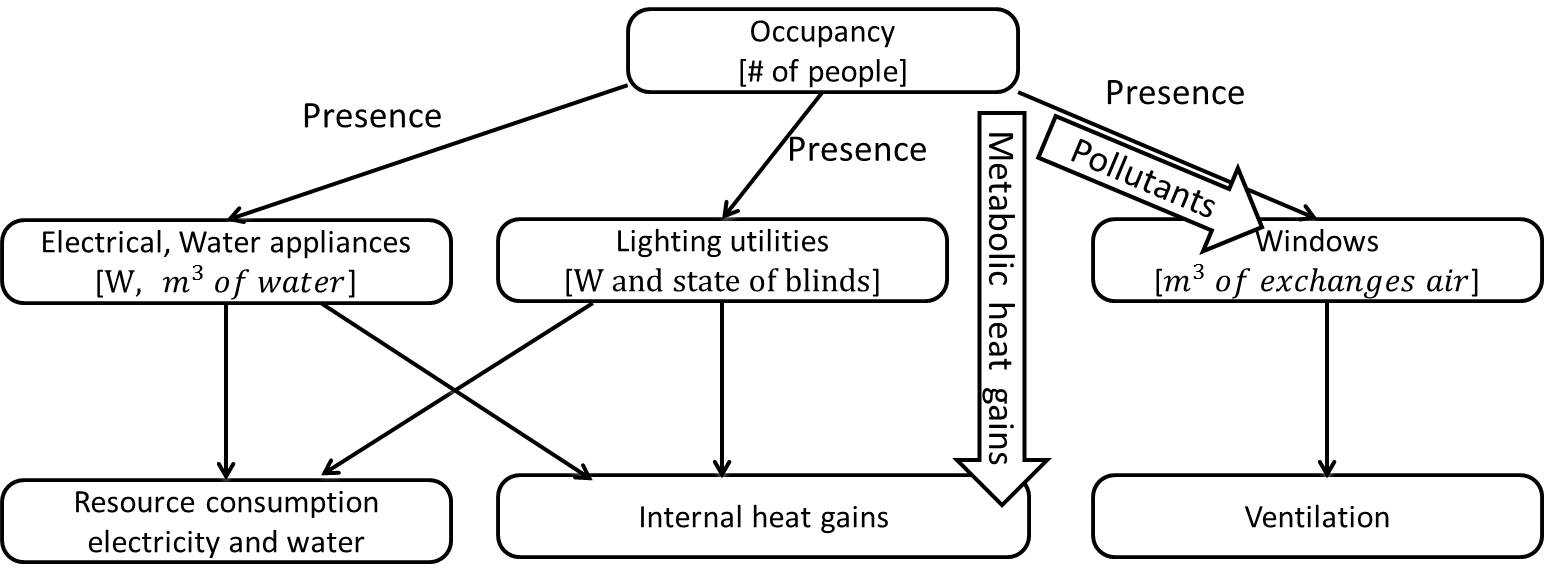
\includegraphics[width=\linewidth]{Figures/Page_presence_scheme.jpg}
  \caption{Outputs of the occupancy model and their later use by stochastic models of occupants’ behaviour. \cite{page_2008}}
  \label{fig:OCC_MODEL}
\end{figure}

Most of the OcP models that are summarized in \citeauthor{page_2008}'s work fit their parameters according to the related presence data. This process, called “calibration process”, was often made by hand or deduced by heuristic techniques. In most cases, the evaluation methods for these models was the measurement of their capacity to reproduce, realistic behavior of the occupants after the calibration process. Having a realistic simulation of occupant presence
is one of the most important aspects for the OcP models, this is because, a lack of an accurate estimation of occupant presence will imply a miscalculation of resources such as water, electric energy and others. Thus, the over- or underestimation of presence is undesirable in the majority of the cases \cite{page_2008, wang_2005, profile_comp_2001}.\\


\citeauthor{wang_2005}, \citeyear{wang_2005} \cite{wang_2005} put into evidence one example of OcP overestimation. In their simulation, they observed peaks of presence in the first hour of the day (which implies overestimation of presence) due to their assumption of the normal distribution of the arrival time in the morning. \citeauthor{wang_2005} were aware of the absent periods of the occupants, and they found that the absence intervals were exponentially distributed and that the coefficient of the exponential distribution for a single office was treated as a constant over the day. To overcome the overestimation problem of presence,  the authors mention the use of empirical distributions for daily events like the arrival in the morning.    


\subsection{Occupancy diversity factors}

Nowadays, one of most the common ways to estimate occupant presence is by using the diversity profiles approach (also called occupancy schedules or occupancy profiles) \cite{profile_comp_2001,davis2010occupancy,duarte2013revealing}(2001, 2010, 2013). This approach consists of daily profiles that are composed of 24-hour representative values. These representative values are a more realistic interpretation of occupant presence because a daily profile does not make assumptions about the probability distribution of daily events such as arrival times in the morning (as it was described before in the example of \cite{wang_2005}). However, this approach could miscalculate the presence of occupants throughout the year when there is a repetition of a subset of profiles that do not consider the temporal variations such as seasonal habits, irregular days (late arrivals or early departures), differences in behavior between weekdays and weekends, and atypical behavior like the presence of people
in office buildings on a weekend \cite{davis2010occupancy}.   \\

To have a more realistic representation of occupant presence, the OcP models would like to be the closest possible to the real behavior of the occupants. However, for simplicity, it is common that the diversity factor for each workday (i.e. usually from Monday to Friday) is treated identically, and weekends treated with a different profile. A typical profile is lower during the absence of the occupants and increases its value during the expected occupancy periods. A maximum factor value is achieved when the maximum expected presence of occupants occurs, or in the case of some types of  HVAC equipment, when weather is over extreme design condition. Duarte et al. 2013 \cite{duarte2013revealing}.  \\

Davis et al. \cite{davis2010occupancy} show examples of OcP profiles of different kinds of buildings. In their work, we can find remarkable differences between workdays for each building type. One example is the library building, where we can see a highest occupancy level on Mondays and a lowest occupancy level on Fridays. For this building, the authors suggested an individual OcP modeling for the following three groups: Monday through Thursday, Friday, and weekend schedules. These groups have what will be called in this work as behavioral coincidence. \footnote{Note that this term will be used in this work. This term indicates a similarity between two or more OcP profiles}      


\subsection{Deterministic and stochastic occupancy factors}
       
\citeauthor{duarte2013revealing} \cite{duarte2013revealing} mention the idea of deterministic and stochastic occupancy factors. According to their criteria, while a deterministic OcP model identifies or creates a standard workday profile which is the same for the whole workweek, a different weekend profile is created for Saturday and Sunday. The deterministic model assumes no change in occupancy schedules throughout the year. On the other hand, a stochastic model uses various probabilistic methods to capture the random nature of individuals’ behavior. Both OcP models are valid for estimating occupancy presence, the former is simple but overestimates occupancy presence when it does not consider variations over all the entire year. The latter might include an OcP miscalculation when there is no consideration of long absence periods such as business trips, vacations and other such things.\\
  

\subsection{Recent studies}

Today, more buildings have ways in which to measure different kinds of variables of interest at their facilities. The evolution of electronic devices allows ubiquitous sensing by using different technologies, as for example Wireless Sensor Network (WSN). This electronic evolution is part of the Internet of Things (IoT) paradigm (2013, 2014 \citep{gubbi2013internet,zanella2014internet}) and offers the ability to measure, infer and understand environmental indicators from different settings. This generation of enormous amounts of data however, must also be analyzed to give a good grasp of the process of interest \cite{gubbi2013internet}.  The IoT concept aims at making the Internet even more immersive and pervasive, so that little by little, the access is easier to devices such as microntrolers, home appliances, surveillance cameras, monitoring sensors actuators, and others. This implies new opportunities for new application in different domains \cite{zanella2014internet}. One application is \textbf{Smart Cities} where there are important issues such as the optimization of the use of resources in the urban context, structural health of buildings, waste management \cite{zanella2014internet}. For example, there is a tendency to believe that in most urban centers around the world, through processing, visualizing, and uploading sensor data from large architecture, when measurements and models are shared between buildings with control systems, will allow one building to shade another or mitigate the so-called urban canyon effect \footnote{Terminology for places where the street is rounded by buildings on both sides creating a canyon-like environment.} \cite{cuff2008urban}. The canyon effect could affect various local conditions (e.g. temperature, air quality, wind and others) of the closest neighborhood, such that in some cases it implies high temperature for the buildings that are inside of the canyon, or bad air quality among others \citep{cuff2008urban,andreou2013thermal}. Sharing the common patterns that describe the behavioral environment of the buildings in the canyon-like environment could mitigate adverse changes on the local conditions in urban canyons \cite{cuff2008urban}. 
   

In the context of Smart Buildings, new studies benefit from the data acquisition facilities that IoT paradigm provides. In a more general vision, the estimation of OcP for estimating resources is part of Smart cities as well. In fact, the consumption of resources, public services, the use of public spaces and the interaction of several systems like traffic and others are linked with presence of people (i.e. urban sensing) in the smart cities context (2007, 2006, 2006)\cite{abdelzaher2007mobiscopes, burke2006participatory, campbell2006people}). Several studies using different sensors have been carried the last decade. \citeauthor{benezeth2011towards,huang2017occupancy}, 2011, 2017 \cite{benezeth2011towards, huang2017occupancy} explain some of these approaches, the challenges and problem for detecting people in indoors environments. Some of the problems are related to the lack of data analysis in primary sensors. For example, PIR (Passive Infrared Sensor) (2013,2013) \cite{duarte2013revealing,nguyen2013energy} cannot differentiate the number of users or know whether if the user is a human or other entity such as a pet or any other animal. Other example is the inconveniences when noise sensors cannot detect low levels of noise coming from the occupants (i.e. when people are quiet) (2013, 2014)\cite{uziel2013networked,kelly2014application}. \citeauthor{benezeth2011towards,huang2017occupancy} summarize two proposals for overcoming the current limitations, the first one recommends the use of multiple low-cost, non-intrusive, environmental occupancy sensors, privileging the use of an independent distributed detectors network combined with a probabilistic data analysis \cite{benezeth2011towards,huang2017occupancy}. The second one recommends the use of more advanced devices such as video cameras which implies a large data storage and privacy concerns  \cite{benezeth2011towards}. Furthermore, sophisticated vision algorithms are needed and they deal with multiple issues like background substraction, tracking and recognition 2013, \cite{sid2013detection}. \citeauthor{huang2017occupancy}, 2017, \cite{huang2017occupancy} propose an approach based on a hybrid sensor (i.e. $CO_2$ sensor and light sensor) to detect the OcP, where this combination of two sensors creates a more robust sensor for detecting OcP. The results indicate that this hybrid combination leads to 
more accurate occupancy detection than only using a $CO_2$ sensor. In literature, one observe that there is a tendency to use the second proposal of \citeauthor{benezeth2011towards}'s work to detect presence, because is considered more robust. We apply this proposal by using the available data of the \textit{$CO_2$, exhausted air temperature, intake air temperature, status of the blind system} of the studied building. We use these variables in order to see the interaction of variables when there is OcP. Since several studies uses $CO_2$ levels as an input to estimate OcP \cite{huang2017occupancy,labeodan2015occupancy,nassif2012} we use the mentioned variables to create multivariate samples \footnote{Multivariate samples are explained in section \ref{sec:MVA}.} in our proposed \textit{GaHMM interactional model} explained in section \ref{sec:interactional_model}. 


\section{Automated Fault Detection and Diagnostic}

\citeauthor{kim2017review}, 2017 \cite{kim2017review} provided a summary of AFDD studies published since 2004. They pointed out that 118 new studies in the past decade were identified and reviewed in their work. The latter work proposes a classification of AFDD methods based on the compilation of previous articles \cite{katipamula2005methods1,katipamula2005methods2}. Basically, there are three big groups of AFDD approaches: \textit{quantitative methods, qualitative methods, and process history-based}. The process history-based AFDD methods
is the most popular approach because they rely on historical data to train models and because of their reduced modeling complexity \cite{kim2017review,katipamula2005methods1}. Our interest is focused on process history-based approaches, since a subcategory of this group (i.e. Black box methods) applies pattern recognition techniques to explain a relationship
between inputs and outputs of a process or a system \cite{kim2017review}. The final idea of these approaches is to  compare the performances of the building over a period of time to what is expected, in this way incorrect operation or unsatisfactory performances can be detected \cite{capozzoli2015fault,katipamula2005methods1}. In this domain of detecting unsatisfactory performances, data mining techniques can be used for this purposes. However, there are few papers that use artificial intelligence and data mining techniques (mostly used in building energy consumption fault detection \cite{capozzoli2015fault,miller2015forensically}). Therefore, we observed  that there still room for applying machine learning, and data mining in this domain. This master thesis attends to contribute to the AFDD literature, with time-dependent cluster task and multivariate pattern recognition (i.e. the three proposed models in section \ref{modeling}).      
  

\section{Data mining process}

Here we include the data mining techniques to use in our approach.

\subsection{Multivariate pattern analysis}
\label{sec:MVA}

Univariate analysis considers one single dependent variable (DV) being measured, and analyses whether the variation of DV is associated with different conditions of interest (i.e. independent variables IV). Each measure is considered as a sample, and the measures of this variable can be represented as a vector. In contrast, multivariate analysis (MVPA) considers multiple dependent variable (DVs) (depending on the nomenclature, it can be called as features or voxels) that are measured and analyzes the relationship with the independent variables (IVs). A sample in MVPA, is therefore, a vector of N values where N is the number of features. In the end, the measurements can be presented by a matrix, that is a two-dimensional, where there are M samples and N features, and the matrix is sized M x N (\citeauthor{baur2007multivariate}, 2007 \cite{baur2007multivariate}). This concept is largely used in our proposition, this help us to defined the observed samples that are explained in section \ref{sec:HHM}. \\  

Depending on the terminology, a pattern can be described as a vector containing the observations of features for a single sample. In a simplistic and generic sense, MVPA includes any analysis where the outcome is dependent on the variability and/or consistency of measurements across samples by features matrix \cite{baur2007multivariate}. \citeauthor{baur2007multivariate} proposed the following typical steps for doing multivariate data analysis:  

\begin{itemize}
\setlength\itemsep{0.1em}
\item[1.] Framing the research question in such a way that it can be modeled mathematically.
\item[2.] Selecting the right statistical model. Every multivariate model searches for certain patterns in 
data. It might miss other patterns. Using different multivariate methods therefore may lead to different results. Among the theoretical questions multivariate analysis can address: \textbf{a)} identifying latent classes; \textbf{b)} causal analysis; \textbf{c)} identifying patterns in time; \textbf{d)} network analysis; and \textbf{e)} multilevel analysis. \footnote{Most multivariate procedures can be viewed as a special case of general linear models (GLM).}
\item[3.] Verifying that assumptions and prerequisites for the chosen statistical procedure are met. 
\item[4.] Preparing data for the specific analysis.
\item[5.] Computing the model using statistical algorithms and methods.
\item[6.] Analysis of the results.
\end{itemize}
 
Some of the previous steps are applied in the following sections. In this study, we applied MVPA because we believe that we can explain in a more meaningful way the building performance/behavior by considering all the variables together (e.g. $CO_{2}$ levels, blind height, cooling energy, etc.) as a single sample. This is observed in models \textit{GaHMM - seasonal} and \textit{GaHMM - interactional}, section \ref{sec:seasonal_model}.    
 
 
%----------------------------------------------------------------------------------------

\subsection{Hidden Markov Model}
\label{sec:HHM}
This section discusses the perils and advantages of using Hidden Markov Model \textbf{(HMM)} and in particular, describe one extension of the HMM called the Guassian Hidden Markov Model \textbf{(GaHMM)}. \footnote{Some authors use GHMM for Generalized Hidden Markov Model. To disambiguate the term, we use GaHMM for Gaussian Hidden Markov Model.} The mathematical notations and details that this work adopts for HMM are in \citeauthor{pfundstein2011hidden}'s work , 2011 \cite{pfundstein2011hidden}. However, some definitions for later purposes are listed here:

\begin{itemize}

\item $\mathbb{O} = (O_1,O_2, ...,O_T )$ is the observed sequence, each observation (i.e. $O_{n \in [1,T]} $) is a sample that can be a number or a vector. $T$ is the total number of the samples. 

\item $\mathbf{K}$ is the number of hidden states for an HMM model. $\mathbf{K} \in \mathbb{N}^+$.

\item $\mathbb{S} = (s_1,s_2, ...,s_T )$ is the hidden state sequence given an observed sequence. Depending on the problem, we can be interested in finding the most likely sequence of hidden states $\mathbb{S}$ that generates/emits the observed sequence $\mathbb{O}$. The hidden sequence $\mathbb{S}$ can be determined by Viterbi's algorithm. \footnote{The words 'emits' and 'generates' is used indiscriminately in HMM literature.}

\item $\pi = (\pi_1, ...,\pi_\mathbf{K}) $ is the initial state probabilities where $\pi_i = P(s_{i=1})$ and $\sum_{i=1}^{\mathbf{K}} \pi_i = 1$.

\item $a_{i,j}$ is the transition probability for going from the hidden state $s_i$ to the hidden state $s_j$. It can be denoted as $a_{i,j} = P(s_{t+1=j} |s_{t = i})$. 
 
\item $\mathbb{A} = \{ a_{i,j}  \mid i \in [1,\mathbf{K}]; j \in [1,\mathbf{K}] \}$ is the transition probability matrix of the hidden states where $\sum_{j=1}^{\mathbf{K}} a_{i,j} = 1$.

\item $b_{k,t}  | t \in [1,T]$ is the probability that a sample $O_t$ is emitted in state $s_k$. Or in other words that, given a hidden state $s_k$, the observed sample $O_t$ was emitted in time $t$ for this hidden state. 

\item $\mathbb{B} = \{b_{k,t}  | k \in [1,K]; t \in [1, T] \} $ is the observation/emission probability matrix where $b_{k,t} = P(O_t | s_{k})$. Typically, a multivariate Gaussian distribution is assumed, but other distributions can be used as well.

\item $\lambda = \{\pi, \mathbb{A}, \mathbb{B} \}$ is the parameter vector that specify an HMM model.

\item The \textbf{limited horizon assumption} claims that the probability of being in a state at time $t$ ($s_t$) depends only on the state at time $t-1$ ($s_{t-1}$). The reasoning underlying this assumption is that the state $s_t$ represents enough summary of the past to reasonably predict the future. Formally: 
\begin{equation}
P(s_t|s_{t-1},s_{t-2},...,s_1) = P(s_t|s_{t-1})
\label{horizon_ass}
\end{equation}

\item The \textbf{stationary process assumption} claims that the conditional distribution over a next state given a current state does not change over time. In other words, it is assumed that state transition probabilities are independent of the actual time at which the transitions takes place. Formally: 
\begin{equation}
P(s_{t_1+1=j}|s_{t_1=i}) = P(s_{t_2+1=j}|s_{t_2=i}) \quad t_1,t_2 \in [2,T] \quad \wedge  \quad t_1 \neq t_2 
\label{stationary_ass}
\end{equation}

\item The \textbf{output independence assumption} is that the current output (observation $O_i$) is statistically independent of the previous outputs (observations $O_{i-1}, O_{i-2}, ..., O_{1} $). Formaly: 
\begin{equation}
P(\mathbb{O} |\mathbb{S}, \lambda) = \prod_{t=1}^{T} P(O_t|s_t,\lambda)
\label{independence_ass}
\end{equation}

\end{itemize}


\begin{figure}[h!]
  \vspace{0.5em} %better style
  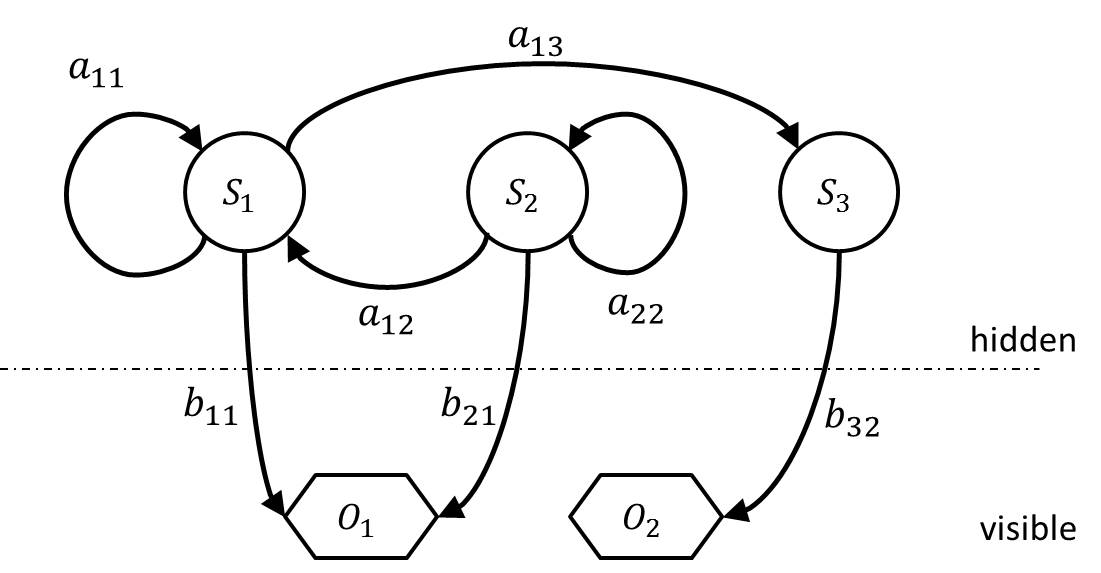
\includegraphics[scale=0.6]{Figures/HMM_simple.jpg}
  \caption[description]{\textbf{HMM Visual representation:} It shows the transition probabilities between three hidden states $\{S_1, S_2, S_3 \}$ and the emission probability transitions $\{b_{11}, b_{21}, b_{32} \}$. Note that the transition probabilities equal to zero are not included, for example: $a_{23}$. Only the observed sequence $O_{t \in [1,T]}$ is observable, the states $\{S_1, S_2, S_3 \}$ that produce the samples are not observable. The emission probability transition $b_{k,t}$ can be any probability function, for example a Gaussian distribution.}
  \label{fig:HHM_MODEL}
\end{figure}

Figure \ref{fig:HHM_MODEL} shows the visual representation of the HMM. It says there is an internal Markov process, that itself cannot be "observed" directly which is called as the "hidden Markov process" (i.e. three hidden states $\{S_1, S_2, S_3 \}$ with their correspondent probability transitions $a_{ij}$). This Markov chain is the responsible for generating observed samples ${O_1, O_2}$ according to the probabilities specified by the matrices $\mathbb{A}$, $\mathbb{B}$ and $\pi$. Once one hidden state is reached, it is said that the state $S_k$ emits an observed sample $O_t$ under the probability $b_{k,t}$. The sequence of hidden states $\mathbb{S}$ that generated the observed sequence $\mathbb{O}$ can be revealed by solving the decoding problem that is explained in section \ref{sec:decoding_HMM}. 




\subsection{Gaussian Hidden Markov Model}

To overcome certain predefined weaknesses of the standard HMM, new ways to combine HMM with other approaches or new models have been proposed (\citeauthor{ghahramani2001introduction}, 2001 \cite{ghahramani2001introduction}). One extension of the HMM model for continuous observation values is the Gaussian Hidden Markov Model (GaHMM). Here we borrow some of its concepts for a better description of this extension \cite{bilmes1998gentle,murphy2002dynamic}. \\

A Hidden Markov Model is a probabilistic model of the joint probability of a collection of random variables $\{ O_1,O_2, ...,O_T \}$ and $\{ S_1,S_2, ...,S_{\mathbf{K}} \}$. Where the $O_t$ variables are either continuous or discrete observations and the $S_k$ variables are hidden and discrete. The term discrete for the hidden states implies that we only have $\mathbf{K}$ possible categorical states. Two assumptions make this model tractable, which are defined in equations \ref{horizon_ass} and \ref{independence_ass}. Furthermore, it is assumed that the underlying 'hidden' Markov chain defined by $P(S_t |S_{t-1})$ is time-homogeneous (i.e. it respects the stationary process assumption, equation \ref{stationary_ass}). The hidden Markov chain is represented by the time-independent stochastic matrix $\mathbb{A}$ and the special case when $t=1$ is described by the initial state distribution $\pi$. Now, if the observations $O_i$ are discrete symbols, we can represent the observation model as the matrix $\mathbb{B}$ where $b_{k,t} = P(O_t|S_k)$, but if the observations $O_i$ are a vector in $\rm I\!R^{L}$, it is common practice to use a continuous probability density function, instead of a set of discrete probabilities. GaHMM represents $b_{k,t}$ using a Gaussian distribution: 

\begin{equation}
P(O_t=y|S_t = x) = \Gamma  (y;\mu_x,E_x) 
\label{g_prob_gua_ec}
\end{equation}

Where $\Gamma  (y;\mu, E) $ is the Gaussian density function with a mean vector $\mu_x$ and the variance covariance matrix $E$ evaluated at $y$:   

\begin{equation}
\Gamma (y;\mu,E) =  \frac{1}{(2\pi)^{L/2} \sqrt{ \parallel E \parallel}} exp \Big[ -\frac{1}{2}(y - \mu)^{\intercal} E^{-1}(y - \mu) \Big]  \quad \quad  \text{\footnotemark} 
\label{density_function_b}
\end{equation} 
\footnotetext{Note that $\intercal$ is the symbol for the vector/matrix transpose and $L$ is the cardinality of $\mu_x$.}


A more flexible representation of the GaHMM model is a mixture of $\mathbf{K}$ Gaussians:

\begin{equation}
P(O_t=y|S_t = x) = \sum_{m=1}^{\mathbf{K}} P(M_t=m|S_t=x) \Gamma(y;\mu_{(m,x)},E_{(m,x)})
\label{mixture_gausssian}
\end{equation}
 
where $M_t$ is a hidden variable that specifies which mixture component to use, and $P(M_t=m|S_t=x) = C(x,m)$ is the conditional prior weight of each mixture component \cite{murphy2002dynamic}. In other words, this is the sum of all mixture components with their correspondent distribution, so that all together it represents the probability of an observed sample $O_t$ occurring at time t when the hidden state is equal to $x$. At the end, each hidden state $S_{i}$ is defined by a mean vector $\mu_x$ with his distribution represented by variance-covariance matrix $E_x$.   


\subsubsection{The three problems to solve using HMM}
\label{sec:problems}

HMM is used to solve three kind of problems that are: the learning, evaluation and decoding problem. The solution of these problems is the core of our proposition. In the modeling process, explained in section \ref{modeling}, one finds the libraries that solve each of them. Basically, our proposition find the best HMM models to discover all the possible patterns into the observed sample $\mathbb{O}$. The theoretical details are explained briefly in this section, and the whole implemented process in section \ref{sec:training_process}. The following explains the general idea of the process:
  
\begin{itemize}
\item Learning/ training process: The HMM model is fitted with the observed samples $\mathbb{O} = (O_1, O_T)$. The definition of the observed samples is very important since it defines the kind of HMM to use.
\item Evaluation process: Here one uses the log probability of $P(\mathbb{O} |\mathbb{S}, \lambda)$ (i.e. equation \ref{independence_ass}), to select the best trained model. The model that fits the best the parameters of $\lambda$ is the one who has the greatest probability.
\item Decoding process: When one obtain the best model, there is a perfect matching between the observed samples $\mathbb{O}$ and the sequences of states $\mathbb{S}$. One says that each hidden state $S_k$ emits one sample $O_i$. This is graphically explained in section \ref{sec:profile_model}. We use this mechanism to cluster similar observed samples.  
\end{itemize}

Here the theoretical details. Using the Markov assumptions (i.e. \ref{horizon_ass}, \ref{independence_ass}, \ref{stationary_ass}), one can answer questions about the observed sequence, the hidden sequence, or the model parameters $\lambda$. These related questions are known as the three basic problems of HMM. This work does not go into detail about these three questions, but the reader is invited to refer to an excellent tutorial in \cite{bilmes1998gentle}, and more related literature of HMM in \cite{haussler1996generalized, ghahramani2001introduction, stamp2004revealing, ramage2007hidden, pfundstein2011hidden}. 


\subparagraph{The Learning Problem}
\label{sec:learning_HMM}

Given an observed sequence $\mathbb{O}$ how can we find the HMM that best fits? HMM has different ways to tune the parameters $\lambda = \{\pi, \mathbb{A}, \mathbb{B} \}$. There are two approaches for the training process, the generative training algorithms and discriminative training algorithms \cite{dymarski2011hidden}. Usually, the solution space of HMMs is coded as a function of $\lambda$ and one can consider two main optimization criteria as being: Maximum Likelihood (ML) and Maximum Mutual Information (MMI). This optimization of parameters $\lambda$ is usually done by gradient algorithms in order to find the maximum likelihood. The Maximum Likelihood Estimation (MLE) can be found by using the Expectation-Maximization algorithm (EM). This algorithm is able to deal with derivatives of the likelihood function with respect to all the unknown values of $\lambda$ by picking arbitrary values for one set of unknown parameters, and then using the previous set, to estimate a second set of parameters, and then apply this procedure recursively until the convergence of parameters. In general, this process generates multiple solutions, so there is no guarantee that the global maximum will be found \cite{dymarski2011hidden}. Our proposed method uses EM algorithm to tune the $\lambda$ parameters, and the best trained model (i.e. the one that get the maximum likelihood) is elected by doing a k-fold cross validation process. This process is explained in \ref{sec:cross}. 


\subparagraph{The Evaluation Problem}
\label{sec:evaluation_HMM}

In general, one of the benefits of HMM is its evaluation property. The question that involves the observed sequence and the parameters of the model is known as the evaluation problem. The question is formulated as follows: What is the probability that the given observations $\mathbb{O} = (O_1,O_2, ...,O_T )$ can be generated by a Hidden Markov Model with parameter $\lambda = \{\pi, \mathbb{A}, \mathbb{B} \}$. In other words: $p(\mathbb{O}|\lambda) = ?$. The solution to this problem is the use of the forward or backward algorithm that finds $p(\mathbb{O}|\lambda)$ in about $K^{2} T$ multiplications \cite{stamp2004revealing}. The solution to this question can be used to evaluate a trained HMM, or it can also suffice just to know whether or not an observed sequence can be generated/emitted by a given HMM, the latter being used in classification problems. In this study, since we are conducting unsupervised fault discovery and are interested in evaluating our trained models and using the best ones, we can perform fault detection.



\subparagraph{The Decoding Problem}
\label{sec:decoding_HMM}

In some cases, one is interested in finding the "most likely" state sequence of the Markov process, given an observed sequence $\mathbb{O} = (O_1,O_2, ...,O_T ) $. Literature defines "most likely" in at least in two ways: 1. "most likely" is defined as the state sequence with the highest probability from among all possible state sequence of length $T$. 2. "most likely" is defined as the state sequence that maximizes the expected number of correct states \cite{stamp2004revealing}. This study is interested in finding the whole state sequence with maximum likelihood. 

Therefore, the problem is defined as: To find an optimal sequence for the underlying hidden Markov model given a HMM with parameter $\lambda = \{\pi, \mathbb{A}, \mathbb{B} \}$ and an observed sequence $\mathbb{O}$. Stated differently, we want to know the "most likely" hidden state sequence that emitted the observed sequence $\mathbb{O}$. To solve this problem the Viterbi algorithm is used. By using Viterbi algorithm, one can find the sub-sequences of an observation sequence O that best matches to a given hidden Markov model. For the present study, this is the way in which the typical daily patterns are discovered and clustered. Finding the most likely hidden state sequence is the way in which we tag days where there is similar pattern across the entire time series.

 
\subsubsection{Advantages and perils of using Hidden Markov Model}

An HMM is a generative, probabilistic model. This model generates distributions by using the available information from the observed sequence. Because of its capacity for detecting sequences, this model is often used for recognition problems that involve sequence recognition such as speech recognition, gesture recognition, information extraction, recognition of Human Genes in DNA and others \cite{ramage2007hidden, seymore1999learning, haussler1996generalized}. \citeauthor{seymore1999learning}, 1999 \cite{seymore1999learning} stated the advantages and perils of HMMs as follow: 

\begin{quote}
"HMM offers the advantages of having strong statistical foundations that are well-suited to natural language domains, handling new data robustly, and being computationally efficient to develop and evaluate due to the existence of established training algorithms. The disadvantages of using HMMs are the need for an a priori notion of the model topology and, as with anystatistical technique, large amounts of training data".
\end{quote}

Later, \citeauthor{ghahramani2001introduction}, 2001 \cite{ghahramani2001introduction} showed that HMMs are a kind of Bayesian Network because it is possible to derive the HMM algorithms from more general algorithms for Bayesian networks. He also explained how to overcome some weakness of HMM models (due to the unconstrained transition matrix $\mathbb{A}$ and the exponential number of states in the model) by creating more general models for HMM such as factorial HMMs and tree-structured HMMs. \\ 


\subsection{Hierarchical clustering}
\label{hierarchical}

Hierarchical clustering seeks to build a hierarchical structure of observed objects in a recursive fashion. Two methods are identified: \textbf{1. Agglomerative.}  This is a "bottom up" approach, each object starts in its own cluster. Then clusters are successively merged until the desired cluster structure is obtained. \textbf{2. Divisive} This is a "top down" approach, all objects belong to one cluster. Then the cluster is divided into sub-clusters, which are successively divided into their own sub-clusters. This process continues until to reach the desired structure \cite{maimon2007soft}. Since the \textit{GaHMM profile} model described in section \ref{sec:profile_model} discovers the existing daily patterns into the time series of the variables, we need an strategy to group cluster profiles in a "bottom up" fashion, creating in this way groups of cluster profiles. There are abundant literature about similarity distances and linkage methods  \footnote{Rules that serve as criteria for joining similar objects} for hierarchical clustering, the reader is invited to see more details about the set of metrics and linkage methods in \cite{saraccli2013comparison,mullner2011modern,maimon2007soft}. We describe in section \ref{sec:hierar_agg}, the use of the hierarchical agglomerative clustering for grouping the discovered cluster profiles.

 

\subsection{Symbolic Aggregate Approximation (SAX) transformation}
\label{section:SAX}

SAX allows the representation of time-series data in words of a finite alphabet $A$. This approach was developed by \citeauthor{keogh2005hot}, 2007 \cite{lin2007experiencing,butler2015sax,keogh2005hot}. The SAX transformation follows this process: The normalized timeseries, Z(t) \footnote{z-scored normalization is applied}, is first broken down into N individual non-overlapping subsequences. This step is known as chunking, and the period length N  is based on a context logical specific period \footnote{Since the interest of this work is to find daily pattern, therefore $N=24$} \cite{lin2007experiencing}. In the next step, each sunsequence of the time series is divided into W equal sized segments. The mean of the points in each small segments is calculated and an alphabetic character from $A$ is assigned according to the table in \ref{table_sax} \cite{lin2007experiencing}. To do this asignation, each mean values that falls in zones between the vertical breakpoints, $B= \beta_1,..., \beta_a - 1$ is substituted by a symbol. Figure \ref{SAX_transf} \cite{lin2007experiencing} exemplify the concept, where the time series (blue line) is transformed into the correspondent word "baabccbc". This approach is used in DayFilter approach \cite{miller2015automated}, which is considered as one of the way to detect daily profiles in the state of the art \cite{kim2017review}. The SAX method can convert time series data with an equivalent symbolic representation for identifying relevant patterns by comparing strings. \citeauthor{miller2015automated}, 2015 \cite{miller2015automated} presented how the SAX method can be implemented to detect the schedules using total building power measurement. \citeauthor{miller2015automated} performed pattern discovery over two different power measurement time series data of the energy consumption of two buildings. His analysis imply among other issues, the identification of discord profiles that implied high corruption of energy \cite{kim2017review, miller2015automated}. The SAX approach is compared against our proposed \textit{GaHMM profile} model in section \ref{comparison_sax_hmm}.


\begin{figure}[h!]
  \vspace{0.5em} %better style
  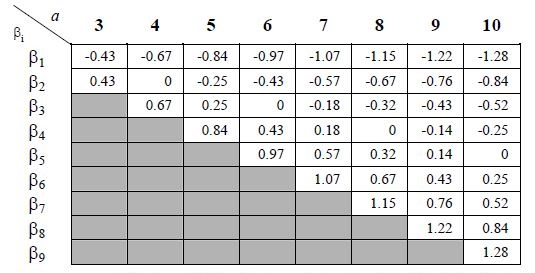
\includegraphics[scale=0.7]{Figures/table_sax.jpg}
  \caption[description]{A lookup table that contains the breakpoints that
divide a Gaussian distribution in an arbitrary number (from 3
to 10) of equiprobable regions}
  \label{table_sax}
\end{figure}

\begin{figure}[h!]
  \vspace{0.5em} %better style
  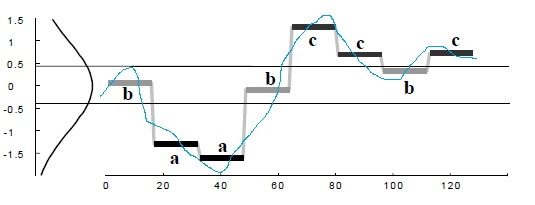
\includegraphics[scale=0.7]{Figures/SAX_transf.jpg}
  \caption{A time series is discretized by first obtaining a PAA approximation and then using predetermined breakpoints to map the PAA coefficients into SAX symbols. In the example above, with n = 128, w = 8 and $A = \{ a, b, c\}$, the time series is mapped to the word baabccbc }
  \label{SAX_transf}
\end{figure} 
 

\section{Data Visualization}

This master thesis does not develop a new data visualization artifact for presenting the discovered information within the multivariate dataset. Developing a new visualization goes beyond our objectives. However, our work uses visualization principles and tools in order to communicate to the reader complex structures of patterns, the interaction between variables, the evaluation of models and the respective results of each section. This task is not a easy task to do since one has to look for visualization that fits the best with the data. In fact, the use of principles, concepts, techniques and theories for data visualization come from multiple backgrounds: programming, web design, semiotic or psychology (\citeauthor{aparicio2014}, 2014 \cite{aparicio2014}). Therefore, choosing one visualization could become a complex situation because it could imply several criteria from different disciplines. In this work, the combination of data mining, and data visualization can be considered as art and science \cite{aparicio2014, kohavi2001data} because there is not strict rules to define which visualization is the most appropriate, and the trial-and-error process is one of the common approaches to use in this domain \cite{kohavi2001data}. Propositions such as Exploratory data analysis (EDA) aims to looking at data for finding descriptive patterns, trends or any hint that help to generate hypothesis of interest of the researcher. However, if this process is made by hand in a high dimensional dataset, it becomes impractical in some cases because of the filtering process \cite{witten2016data}. We believe that the use of data mining techniques in combination with the appropriated visualizations are a powerful tool for knowledge discovery. The reader will see the use of existing visualization artifacts for different purposes. For example, box plots \cite{williamson1989box} are used for a visual evaluation of the cluster quality of cluster profiles in section \ref{sec:eval_all}. Other concept such as the calendar visualizations \cite{van1999cluster} are needed in order to see the distribution of clusters in section \ref{sec:seasonal_model}, and others uses. We expect by the use of data visualizations be able to discover the behavior of the building and represent it in the best possible way. 

\subsection{Hierarchical Edge Bundles}
\label{sec:edge}


Hierarchical Edge Bundles visualization was proposed by \citeauthor{holten2006hierarchical}'s work (2006, \cite{holten2006hierarchical}). This visualization is a compound graph that is based on visually bundling the adjacency edges, i.e., non-hierarchical edges, together. In this way, two or more nodes are joined by using polylines that are bended using a B-spline curve for more readability. This tree visualization based technique can be used in conjunction with other visualizations to express different concepts. Figure \ref{fig:edge} shows an example where this visualization displays adjacency relations between nodes. Colors in the linkage line provide more information about the connection between nodes. 



\begin{figure}[h!]
  \vspace{0.5em} %better style
  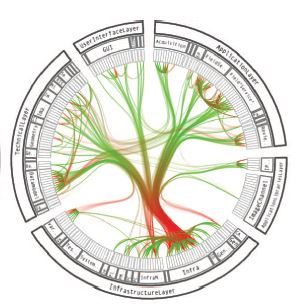
\includegraphics[scale=0.7]{Figures/edge.jpg}
  \caption[description]{Radial layout construction of hierarchical edge bundles}
  \label{fig:edge}
\end{figure}


In our case, we use this visualization to represent the connection between the variables (time series of the measurements) in the building, this can be appreciated as an information visualization who explains the existing linear correlation between variables (i.e. nodes). This visualization was used for the interactional model where each node is a variable of the building dataset and each linkage line represent the linear correlation between them, refer section \ref{sec:interactional_model} for more details. Other variations and more layouts of this visualization are explained in \cite{holten2006hierarchical}. \footnote{Library available on \url{https://bl.ocks.org/mbostock/7607999}}

   
% Chapter 3
\chapter{Monitored Building Dataset} % Main chapter title
\label{Chapter3} % For referencing the chapter elsewhere, use \ref{Chapter2} 
\minitoc
%----------------------------------------------------------------------------------------

%% Define some commands to keep the formatting separated from the content 
%\newcommand{\keyword}[1]{\textbf{#1}}
%\newcommand{\tabhead}[1]{\textbf{#1}}
%\newcommand{\code}[1]{\texttt{#1}}
%\newcommand{\file}[1]{\texttt{\bfseries#1}}
%\newcommand{\option}[1]{\texttt{\itshape#1}}

%----------------------------------------------------------------------------------------

This chapter is devoted to the description of the multivariate building dataset and the way in which we manage the time series data. The first section describes the provided raw data, the next section describes the general information of the office building, and finally, we explain how we dealt with the provided time series using a Big-Data database.


\section{Building Dataset - Case Study}

The studied dataset was provided by Synergy BTC AG \footnote{http://www.synergy.ch/} which is a consulting agency with focus on Software-as-a-Service for buildings, located in Bern, Switzerland. A visual interaction tool using this dataset was proposed by \citeauthor{roman2015}, \citeyear{roman2015} \cite{roman2015}. Relevant information relative to this building was taken from that study, and is presented in the following sections. 

\section{Office Building Information}   
\label{general_information}

The monitored building is located in eastern Switzerland. Figure \ref{fig:building_model} shows a model of the building. Table \ref{tab:general_information} summaries general information of the building. Additional information referring to the internal systems and zones are described in this section.  

% Table generated by Excel2LaTeX from sheet 'Hoja5'
\begin{table}[htbp]
  \centering
  \tiny
  \caption{General information of the building.}
    \begin{tabular}{|l|l|rrr}
\cline{1-2}\cline{4-5}    \multicolumn{2}{|c|}{\textbf{Information on building use and system technology}} & \multicolumn{1}{r|}{} & \multicolumn{2}{c|}{\textbf{Space (zoning) per floor}} \bigstrut\\
\cline{1-2}\cline{4-5}    Gross floor area & 9560 $m^2$ & \multicolumn{1}{r|}{} & \multicolumn{2}{l|}{13 office areas (mostly open space)} \bigstrut\\
\cline{1-2}\cline{4-5}    Number of floors: & 3,    & \multicolumn{1}{r|}{} & \multicolumn{2}{l|}{6 meeting rooms} \bigstrut\\
\cline{1-2}\cline{4-5}    Location: & Eastern Switzerland, indutrial area with& \multicolumn{1}{r|}{} & \multicolumn{2}{l|}{5 border zones (traffic area, toilet, stairs)} \bigstrut\\
\cline{1-2}\cline{4-5}    Use:  & Office and administrative building &      &      &  \bigstrut\\
\cline{1-2}    \multicolumn{1}{r}{} & \multicolumn{1}{r}{} &      &      &  \bigstrut\\
\cline{1-2}    \multicolumn{2}{|c|}{\textbf{Building Shell}} &      &      &  \bigstrut\\
\cline{1-2}    Outside Walls & U = 0.24 W/m2K, massive &      &      &  \bigstrut\\
\cline{1-2}    Glazing & Uf = 1.1 W/m2K, Ug = 0.65, g = 0.40 &      &      &  \bigstrut\\
\cline{1-2}    Interior walls: & U = 2.0 W/m2K, lightweight &      &      &  \bigstrut\\
\cline{1-2}    \end{tabular}%
  \label{tab:general_information}%
\end{table}%

\begin{figure}[h!]
  \vspace{0.5em} %better style
  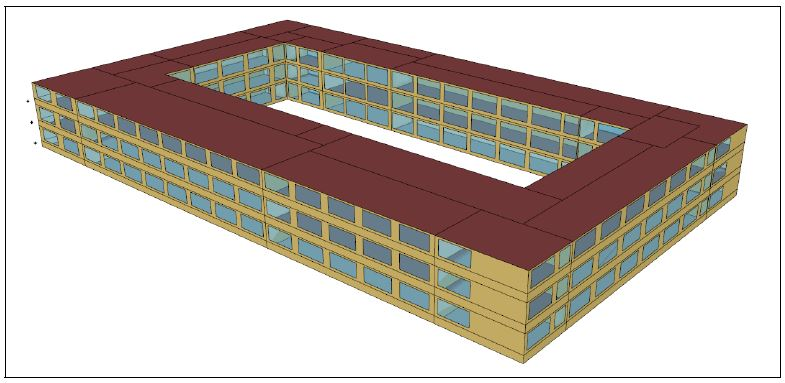
\includegraphics[scale=0.4]{Figures/building_model.jpg}
  \caption{Model of the building \cite{roman2015}}  
  \label{fig:building_model}
\end{figure}

\paragraph{Zoning map per floor} Figure \ref{fig:zoning} shows the room layout for a floor of the office building. It is divided into three different zones: meeting rooms (red), office areas (green) and border zones (blue). For every floor, the zoning is the same.

\begin{figure}[h!]
  \vspace{0.5em} %better style
  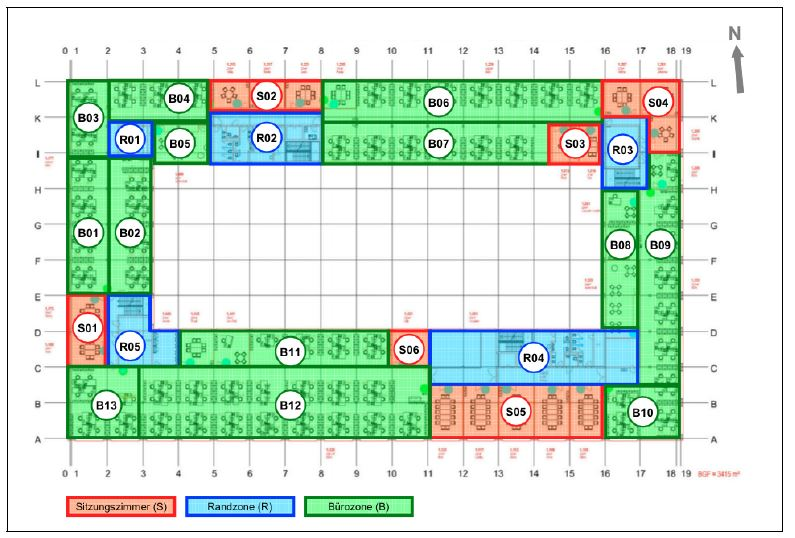
\includegraphics[scale=0.6]{Figures/zoning.jpg}
  \caption{Zoning for each floor \cite{roman2015}}  
  \label{fig:zoning}
\end{figure}

\paragraph{Mechanical Ventilation System} The studied building has two mechanical ventilation systems. The yellow area for the North-East zone and the blue area for the South-West zone (see figure \ref{fig:ventilation}). 

\begin{figure}[h!]
  \vspace{0.5em} %better style
  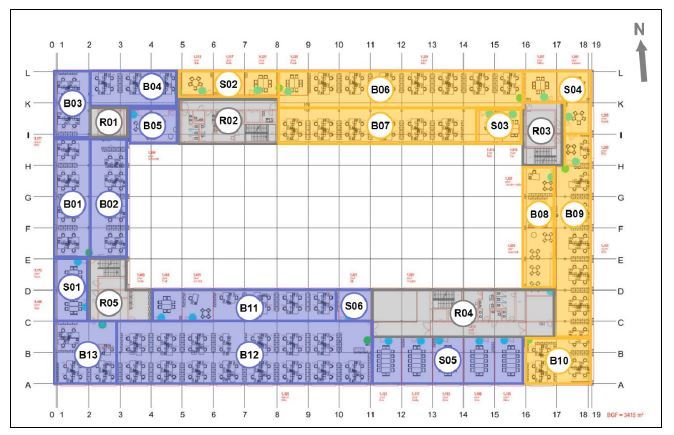
\includegraphics[scale=0.6]{Figures/ventilation.jpg}
  \caption{Mechanical ventilation systems per floor \cite{roman2015}}  
  \label{fig:ventilation}
\end{figure}

\paragraph{Heating and Cooling Systems} The studied building has two thermally-activated building systems (TABS). The red area for the North-East zone and the green area for the South-West zone (see figure \ref{fig:heating}). Each TABS supplies all floors of the corresponding building zone. There are some differences in the zoning of the mechanical ventilation systems and the heating and
cooling system. For example, room B10 is in the north/east zone of the ventilation system, but
in the south/west zone of the heating and cooling system.  

\begin{figure}[h!]
  \vspace{0.5em} %better style
  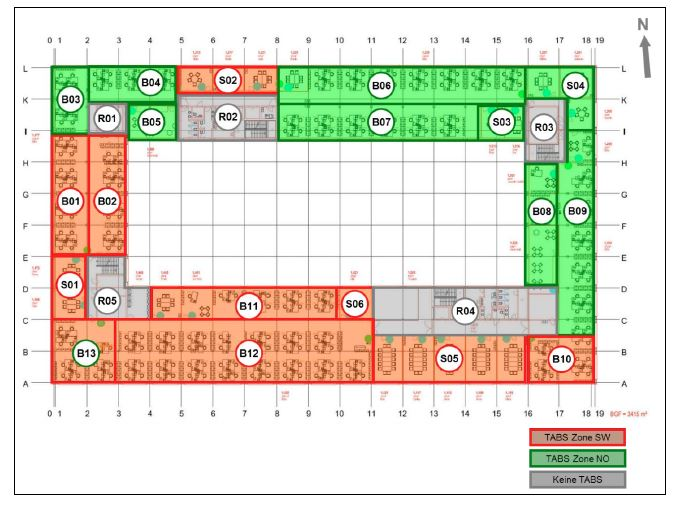
\includegraphics[scale=0.6]{Figures/heating.jpg}
  \caption{TAB systems per each floor \cite{roman2015}}  
  \label{fig:heating}
\end{figure}

\paragraph{Humidity and temperature in rooms}

Temperature and humidity are measured in 4 rooms of each floor. Therefore 12 variables named with the name of room are available in this dataset according to figure \ref{fig:temperature}.  

\begin{figure}[h!]
  \vspace{0.5em} %better style
  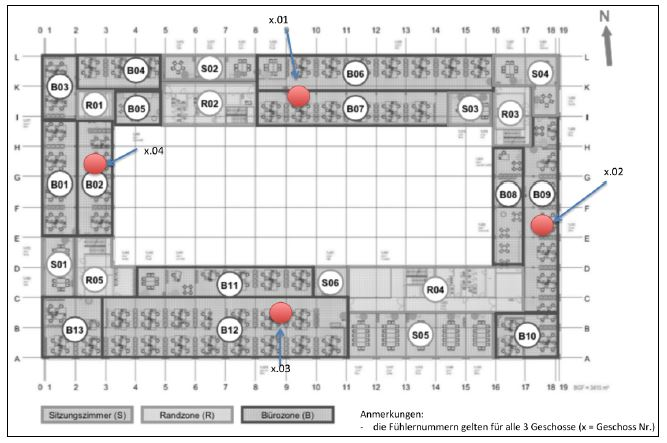
\includegraphics[scale=0.6]{Figures/temperature.jpg}
  \caption{Mechanical ventilation systems per floor \cite{roman2015}}  
  \label{fig:temperature}
\end{figure}


\section{Dataset handling}

The provided dataset has 64 variables with a time range of 3 years, from mid of 2012 until mid of 2015 with hourly time resolution. This implies 25943 registers per variable giving more than 1.6 million measurements. These 64 variables were associated according the provided information explained in section \ref{general_information}.  Table \ref{tab:variable_sum} summarizes the different categories of variables in the building dataset. The complete list of variables is included in the annex \ref{AppendixA}. Each category collects variables of the same type, same internal subsystems or that belong to the same spatial information zone according to section \ref{general_information}. Additionally, the dataset has been enriched with outdoor weather data. The buildings nearest weather station is Zurich-Kloten, for which the data has been acquired from the \textit{Bundesamt fur Meteorologie und Klimatologie Meteo Schweiz}. The variables are outdoor temperature (°C), precipitation (mm) and sunshine hours (min). More information about how the weather temperature changes in Switzerland is in  \cite{rebetez2008monthly}.
   
\begin{table}[htbp]
  \centering
  \scriptsize
  \caption{Variable categories within the Data-set}
    \begin{tabular}{|l|l|}
    \hline
    \multicolumn{1}{|c|}{\textbf{Variable name}} & \multicolumn{1}{c|}{\textbf{Unit}} \bigstrut\\
    \hline
    CO2 exhaust air & ppm \bigstrut\\
    \hline
    Humidity exhaust air & \% \bigstrut\\
    \hline
    Room humidity & \% \bigstrut\\
    \hline
    Temperature exhaust air & °C \bigstrut\\
    \hline
    Temperature intake air & °C \bigstrut\\
    \hline
    Room Temperature & °C \bigstrut\\
    \hline
    Outdoor Temperature & °C \bigstrut\\
    \hline
    Blinds status & 0/1 \bigstrut\\
    \hline
    Cooling TABS & kWh \bigstrut\\
    \hline
    Heating TABS & kWh \bigstrut\\
    \hline
    Sunshine presence per hour & minutes (min) \bigstrut\\
    \hline
    Precipitation level & mm \bigstrut\\
    \hline
    Blinds height & \% (100\% closed, 0\% open) \bigstrut\\
    \hline
    Blinds angle & \% (100\% closed, 0\% open) \bigstrut\\
    \hline
    \end{tabular}%
  \label{tab:variable_sum}%
\end{table}%



\subsection{Building Zones Category}
We divided the building dataset into coming from one of two main spatial zones in the building (i.e. North-East and South-West zone), according to the information provided by Synergy BTC AG. These zones are associated to two different mechanical ventilation and TABS systems. We associated each variable (i.e. time series of the measurements) to the according zone and created a metadata table that is included in \ref{sec:metadata_t}. Field \textit{breakout\_group} uses the codes $A\_\ast$ for the North-East zone and the codes $B\_\ast$ for the South-West zone. 
  
% Table generated by Excel2LaTeX from sheet 'Hoja6'
\begin{table}[htbp]
  \centering
  \scriptsize
  \caption{Extract of the proposed metadata table.}
    \begin{tabular}{|l|l|l|l|l|l|l|}
    \hline
    \rowcolor[rgb]{ 0,  0,  0} \textcolor[rgb]{ 1,  1,  1}{\textbf{tagname}} & \textcolor[rgb]{ 1,  1,  1}{\textbf{alias}} & \textcolor[rgb]{ 1,  1,  1}{\textbf{orientation}} & \textcolor[rgb]{ 1,  1,  1}{\textbf{category}} & \textcolor[rgb]{ 1,  1,  1}{\textbf{breakout\_group}} & \textcolor[rgb]{ 1,  1,  1}{\textbf{alias\_breakout\_group}} & \textcolor[rgb]{ 1,  1,  1}{\textbf{units}} \bigstrut\\
    \hline
    \rowcolor[rgb]{ .851,  .851,  .851} V005\_vent01\_CO2 & CO2 Ventilation NE & NE   & CO2  & A    & CO2 Ventilation NE & ppm \bigstrut\\
    \hline
    V022\_vent02\_CO2 & CO2 Ventilation SW & SW   & CO2  & B    & CO2 Ventilation SW & ppm \bigstrut\\
    \hline
    \rowcolor[rgb]{ .851,  .851,  .851} V037\_tabs\_cold\_SW & Cooling tabs SW & SW   & Cooling & B\_1 & Cooling SW & kWh \bigstrut\\
    \hline
    V075\_tabs\_cold\_NO & Cooling tabs NE & NE   & Cooling & A\_1 & Cooling NE & kWh \bigstrut\\
    \hline
    \rowcolor[rgb]{ .851,  .851,  .851} V034\_tabs\_warm\_SW & Heating tabs SW & SW   & Heating & B\_2 & Heating SW & kWh \bigstrut\\
    \hline
    \end{tabular}%
  \label{tab:Extarct of the Metadata}%
\end{table}%


\subsection{Building measures - Time Series}
\label{sec:dealing}
Script \ref{eq:script} shows how the time series are stored in the database. This script represents a register where variable is the key and the numeric value is the measure of the variable at time equal to timestamp. Our approach adopts a Big-Data database that uses JSON-like documents with schemas. Each register is a JSON document with keys like the timestamp, name of the variable, epoch\footnote{ Unix epoch (or Unix time or POSIX time or Unix timestamp) is the number of seconds that have elapsed since January 1, 1970 (midnight UTC/GMT), not counting leap seconds (in ISO 8601: 1970-01-01T00:00:00Z).}, and others. The flexibility and scalability that Big-Data offers, allows us to retrieve high volumes of data quickly and store complex structures like nested JSON objects. 

\begin{equation}
\scriptsize
\label{eq:script}
\begin{array}{llcl}
\{ &  &  &  \\ 
& timestamp & : & 2012-06-23 \quad 01:00:00 \\	
& epoch & : & 1340406000.0 \\	
 & variable1 & : & 142.25 	\\	
 & variable2 & : & 123.45 	\\	
 & ... &  &  	\\	
 & variablen & : & 123.45 	\\
\} & & & \\
\end{array}
\end{equation}

In our approach, we include the epoch time to the existing dataset to manipulate the time series. This is one simple way to query the time series using ranges of time in a time series dataset. For example, script \ref{scr:query} indicates a NOSQL expression \footnote{This is MongoDB syntax, manual available on \url{https://docs.mongodb.com/tutorials/}} for asking values of a time series within the time range defined by the key \textit{epoch}. \textit{db.timeseries} is the collection of JSON documents that contains the time series of the dataset. The reserved words \textit{\$gte, \$lte} define the time range (i.e. greater than equal to 1412204098 and lower than equal to 1412204099) of the requested variables \textit{variable\_1, ..., variable\_n}. 

\begin{equation}
\scriptsize
\label{scr:query}
\begin{array}{rlll}
db.timeseries.find(\{ &  &  &  	\\
	epoch : \{ &&  &			\\
		&  \$gte&:& 1412204098, 	\\
		&    \$lte&:& 1412204099 		\\
		& \}     \\
     	\},\{& & 						\\
	 variable\_1 & : & True, &		\\    
    	..., & &	&			\\
    	variable\_n & : &  True 		\\
    	\}) \\
\end{array}
\end{equation}

Another proposition from the last script uses a list of timestamps as is showed in script \ref{eq:script2}\footnote{One common framework that facilitates similar operations for manipulating the time series is included as \textit{rs\_common\_framework\_v4.py}.}. \textbf{An important remark} to do is that the NOSQL queries do not guarantee a chronological order of the requested elements by default. Methods to order the requested data are needed, this is a very important aspect to consider when one uses time series, especially for the training process as it is explained in section \ref{sec:cross}. 

\begin{equation}
\scriptsize
\label{eq:script2}
\begin{array}{rlll}
db.timeseries.find(\{ &  &  &  	\\
	timestamp : \{ &&  &			\\
		&  \$in &:& [$'2012-12-21', '2012-12-23', ...$], 	\\
		& \}     \\
     	\},\{& & 						\\
	 variable\_1 & : & True, &		\\    
    	..., & &	&			\\
    	variable\_n & : &  True 		\\
    	\}) \\
\end{array}
\end{equation}
 
Finally, we show in figure \ref{fig:big_data_example} an example of JSON objects stored in the Big-Data database. It shows the power of this approach where key/value pairs are nested. This provides flexibility to our data models, facilitating the storage and the retrieve of complex objects. 
  

\begin{figure}[h!]
  \vspace{0.5em} %better style
  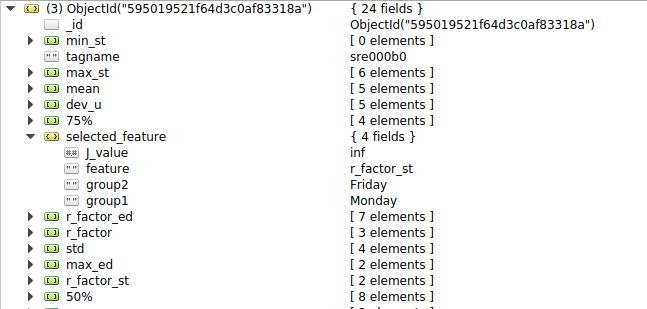
\includegraphics[scale=0.6]{Figures/DataBase_example.jpg}
  \caption{Example of JSON objects stored in the Big-Data database.}  
  \label{fig:big_data_example}
\end{figure}

% Chapter 4
\chapter{Methodology} % Main chapter title
\label{Chapter4} % For referencing the chapter elsewhere, use \ref{Chapter2} 
\minitoc
%----------------------------------------------------------------------------------------

%% Define some commands to keep the formatting separated from the content 
%\newcommand{\keyword}[1]{\textbf{#1}}
%\newcommand{\tabhead}[1]{\textbf{#1}}
%\newcommand{\code}[1]{\texttt{#1}}
%\newcommand{\file}[1]{\texttt{\bfseries#1}}
%\newcommand{\option}[1]{\texttt{\itshape#1}}
%----------------------------------------------------------------------------------------

This chapter is devoted to the description of the software framework developed to solve the problem proposed in \ref{Chapter1}. This work proposes a solution based on Big-Data database, python scripts and exploratory visualizations that allows a solution using Gaussian Hidden Markov Model and hierarchical agglomerative clustering. Finally, at the end of this chapter, we evaluate each of the proposed models to observe the different results that we achieve with each one.

\section{Software Framework}

\paragraph{Identifying the problem scenario}
We consider that the unsupervised fault detection by using machine learning in a multivariate building dataset is a problem that falls in different domains. Regarding the variety of the time series, we consider this problem as a Big-Data problem, since IoT \footnote{IoT is including building and industrial control systems. There is still a question: 'Will we have a smart BAS in the future or is it just part of the IOT?'} is allowing to collect data from ubiquitous sensors, therefore criteria of volumen, variety and velocity are present \cite{george2014big,gubbi2013internet}. Regarding the discovery process of daily profiles, each daily profile is a sub-sequence of the whole trend, and finding the common patterns in the whole trend is analogous to the sub-sequence analysis of DNA sequences, for instance \cite{haussler1996generalized, ghahramani2001introduction, stamp2004revealing, ramage2007hidden, pfundstein2011hidden}. Finally, regarding data mining and visualization mechanisms, we consider that this problem requires effective techniques for knowledge discovery and expressive data visualization artifacts that fits the data \cite{witten2016data,aparicio2014, kohavi2001data}.   

\paragraph{Proposed solution}
We use MongoDB \footnote{For more information: \url{https://www.mongodb.com/what-is-mongodb}} database for having a smart manage of the dataset, the measures and calculations are stored as JSON-like documents allowing flexibility to save/retrieve the data as it was explained in section \ref{sec:dealing}. The architecture of the proposed solution is a traditional three-tier architecture powered by Python's scripts: a big-data database, an application web server and the front-end tier that is the browser's user. Figure \ref{fig:framework} shows the flow of information. The data processing step is done by a transversal script \footnote{script in: /Thesis\_project/lib/rs\_common\_framework\_v4.py} that provides the primitive methods for the all the different modules that are connected. The proposed solution allows the following data mining actions:

\begin{itemize}
\item[a] Raw Data Screening process: Filter values that do not belong to measuring process of the variable.
\item[b] Correlation analysis of variables: Construct a matrix of linear correlation of the variables of the multivariate dataset. \footnote{This process is explained inside of the interactional model, section \ref{sec:interactional_model}}
\item[c] Feature selection process: Calculate the gain of information of an arbitrary feature.
\item[d] Modeling process: The training process of the models, the best models are stored for latter uses. \footnote{ GaHMM models are saved as \textit{.pkl} files in folder: \textit{/Thesis\_project/HMM\_models/Final\_models}. The description of each model is in \textit{description\_model.txt.} }
\item[e] Visualization process: Two visualization mechanism are proposed. \textbf{1.} \textit{Jupyter notebook} \footnote{We use the python version. More available information in \url{http://jupyter.org/}.} is an open-source web application that allows to create and share documents that contain live code, equations, visualizations and explanatory text. \textbf{2} Flask web server \footnote{Web server is implemented using Flask for Python. \url{http://flask.pocoo.org/}} is an open-source web framework that is based on Werkzeug, Jinja 2. This micro-framework is compatible with other libraries like \textit{queue.js, jQuery.js, d3.js, bootstrap.js} that are used to generated personalized information visualizations. 

\end{itemize}

\begin{figure}[h!]
  \vspace{0.5em} %better style
  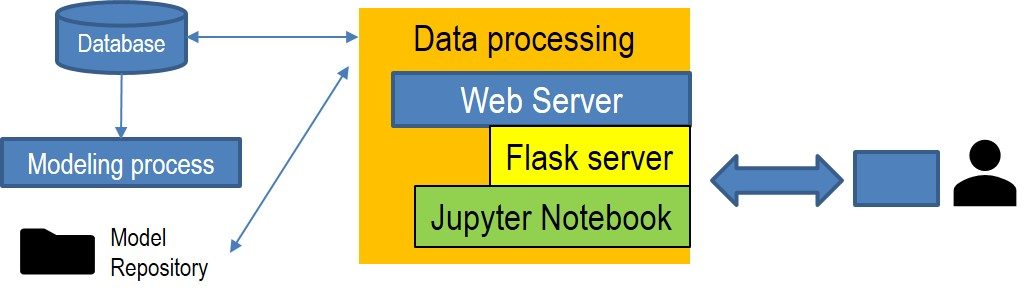
\includegraphics[scale=0.4]{Figures/framework.jpg}
  \caption{Software framework schema}
  \label{fig:framework}
\end{figure}

Figure \ref{fig:structure} shows the implemented collection of JSON documents that were created for each proposed module according to the last list of data mining actions, each of them are explained in details in the next sections.

\begin{figure}[h!]
  \vspace{0.5em} %better style
  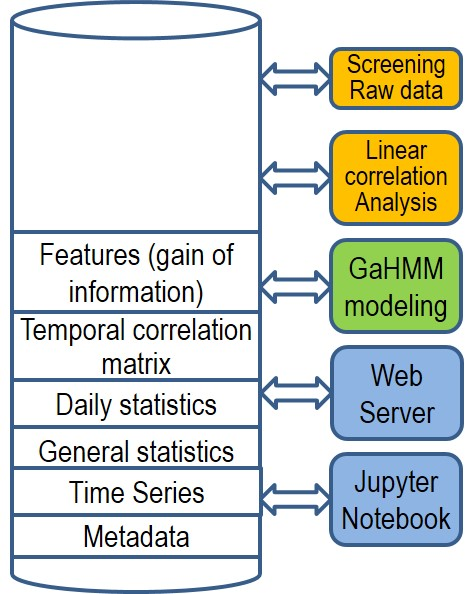
\includegraphics[scale=0.4]{Figures/database_structure.jpg}
  \caption{Implemented collections for saving time series and results}
  \label{fig:structure}
\end{figure} 
 
%We believe that the occupants behavior is a sequence of events during the day, and those sequences can be interpreted as states. For example, consider the following states: arrival at the office, breakfast (or small break), first working period, lunch, second working period, departure from the office. These states are a common sequence for people that work in an office building. We consider atypical days, those day where one or more of these states were skipped.  



\section{Raw Data Screening process}

The raw data screening process is an important step to do before performing any action over the time series dataset. Aspects like the definition of limits and the quality of the data are important issues to know before starting the knowledge extraction process \cite{miller2015forensically}. The raw data screening process aims to clean the dataset in order to offer a good quality for the next phases of the knowledge extraction process. Filter out outliers before applying data mining techniques is commonly applied \cite{miller2015forensically, capozzoli2015fault,lin2003symbolic,kohavi2001data,lin2007experiencing}. One typical approach is by using the $3\sigma$'s (also called six sigma) rule \cite{wiborg2014applied,miller2015automated} or the use of Interquartile range analysis \cite{bickel2015mathematical}. In our approach we use the $3\sigma$'s and propose a new way to spot outliers by using the concept of quartiles. These two approaches are explained after reviewing literature about unsupervised outlier detection. 

\subsection{Unsupervised Outlier detection}

\citeauthor{zimek2014ensembles}, 2014 \cite{zimek2014ensembles} explain the challenges and some popular approaches used for unsupervised outlier detection. The fact that, there is no consensus on the definition of an outlier makes this task hard to do and evaluate. Clearly, the definition of an outlier is subjected to nature of the data. For example, for a time series an outlier may be related to the frequency, amplitude of the variable, or any other criteria such as the number of peaks. Therefore, there is no general outlier detection algorithm, each algorithm is able to detect outliers according to the particular criteria that the researcher is interested in. Nevertheless, \citeauthor{zimek2014ensembles}, 2014 \citep{zimek2014ensembles}, explain the idea of integrating various different outlier detection results, and in this way, the collection of approaches will detect the all most likely outliers.


We apply these two approaches to automatically set the limits of the variables without having any previous knowledge of each variable. These two methods determine the upper and the lower limit ($\textbf{UpL}, \textbf{LoL}$) of a variable, such that we can spot outlier values that are outside of the range $[LoL,UpL]$ \footnote{These outlier values can be associated with noise, inaccuracies, mistaken measures, unwanted deviation due to instrument decalibration and others.}. An easy way to spot unwanted values is by plotting the variable of interest as a trend line, and apply a visual filter. This approach becomes impractical when we deal with large time series and a big number of variables.  Therefore, we need more practical ways to find the variable limits and spot unwanted values. We apply the proposed methods over variables that might not have fixed limits, so that a statistical analysis allows the automatic definition of $\textbf{UpL}$ and $\textbf{LoL}$, after which we can spot extreme atypical values. In other cases, where the limits are explicit (e.g. relative humidity \%) the definition of the limits is not needed, but these approaches are able to spot outliers anyway. \\

Both approaches are based on: \textit{a)} six sigma and \textit{b)} percentile analysis. The first approach fits very good when the measures of a variable follow a Gaussian distribution and belong to a controlled process. The second approach is more general and can be fitted to measures that do not necessarily follow a Gaussian distribution.
  

\paragraph{Six sigma approach}

Details of this approach are shown in figure \ref{fig:six_sigma}. Basically, this approach spots values that are significantly different from the suggested/expected trend,\footnote{This can be subjective depending on the field, it can be that having peaks in the trend is a normal part of the process} that is the detected values $z$ do not belong to the range limited by a Lower Control Limit ($LCL$) and an Upper Control Limit ($UCL$), i.e. $z \not \in [LCL, UCL]$. This approach is based on the three sigma rule, and expresses a conventional heuristic that nearly all values are taken to lie within three standard deviations of the mean  \cite{wiborg2014applied,miller2015automated}. In other words, almost all the possible values for a variable that follows a normal distribution are in an interval of six sigma: $[\mu - 3\sigma, \mu + 3\sigma]$. Where $\mu$ is the mean of the variable, $\sigma$ is the standard deviation, and therefore $LCL = \mu - 3 \sigma$ and $UCL = \mu + 3\sigma$. \\

\begin{figure}[h!]
  \vspace{0.5em} %better style
  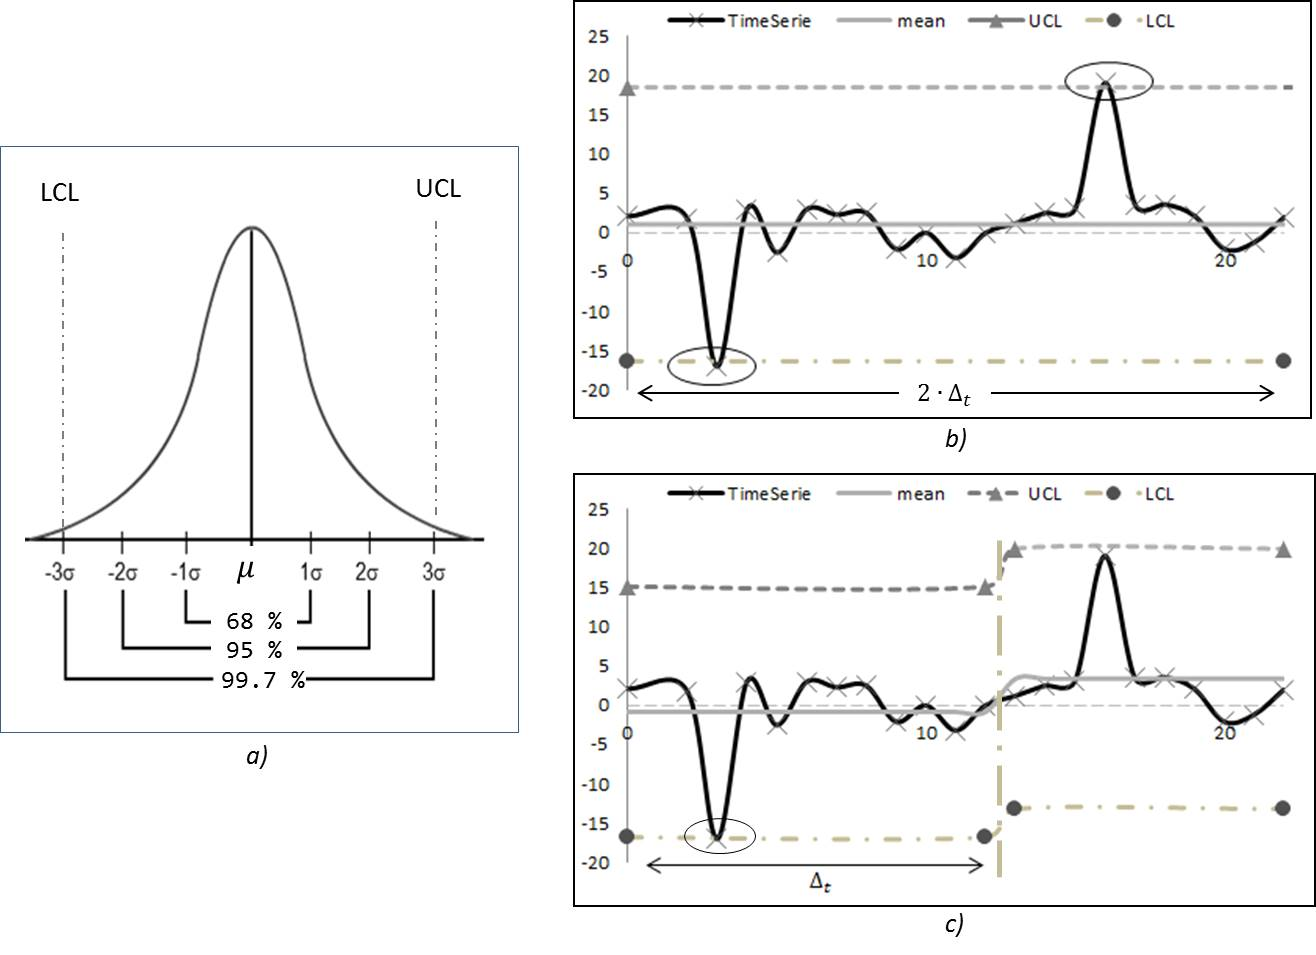
\includegraphics[scale=0.5]{Figures/Six_sigma_example.jpg}
  \caption{\textit{a)} \textbf{The 3$\sigma$'s rule}: There is a 99.7\% probability that the variable values belong to the interval $[LCL,UCL]$. \textit{b)} Six sigma approach for a time series with fixed LCL and UCL limits. Two spotted values (in the ellipse) are considered as outlier values. \textit{c)} Six Sigma approach with a windowing of $\Delta t$ size. The LCL and UCL limits are not fixed and change according to the values inside of the window.  }
  \label{fig:six_sigma}
\end{figure}

In Figure \ref{fig:six_sigma}{\color{red} .\textit{b)}}, one can observe that the $6\sigma$'s approach detects two outlier values for a window of size $2\Delta_t$, while in Figure \ref{fig:six_sigma}{\color{red} .\textit{c)}}, the same approach for a window of size $\Delta_t$ only detects one outlier value in the first window and the other, in the second window, is not detected. We observe in the experiments that the window size affects the detection of outlier values. We notice that the bigger the window is, the more chance there is to detect general outliers, but in contrast, the chance of detecting local outliers is low. We also observe that the smaller the windows is, the less general outliers we can detect. Therefore, having a good definition of the window size is critical for this approach.


\paragraph{Percentile analysis approach}

shows the use of percentile analysis for spotting
outlier values (marked inside the ellipses). This proposed approach determines the LoL and
UpL limits by a linear regression over extreme selected (or rather “selected extreme...”?) percentiles. In this example, we select



Figure \ref{fig:percentile}{\color{red} .\textit{c)}} 
shows the use of percentile analysis for spotting 
outlier values (marked inside the ellipses). This proposed approach determines the \textit{LoL} and \textit{UpL} limits by a linear regression over selected extreme percentiles. In this example, we select the percentiles $\mathbf{P}_l = [P_{5}, P_{10}, P_{15}, P_{20}, P_{25}]$ for the $LoL$ limit, and the percentiles $\mathbf{P}_u = [P_{75},P_{80},P_{85},P_{90},P_{95}]$ for the $UpL$ limit. Two trends are defined using the mentioned percentiles: 
\begin{itemize}
\item[•] The $up\_le$ trend conformed by $up\_le(x) = \mathbf{P}_u$ and $x=[0.75, 0.8, 0.85, 0.9, 0.95]$.
\item[•] The $lo\_le$ trend conformed by $lo\_le(x) = \mathbf{P}_l$ and $x=[0.05, 0.1, 0.15, 0.2, 0.25]$.
\end{itemize}

When we apply a linear regression over each trend, we find the predicted values for the points $x= 1 \to up\_le(x)$ and $x = 0 \to lo\_le(x)$. These values define the $UpL$ and $LoL$ limits respectively. These can be observed in Figure \ref{fig:percentile}{\color{red} .\textit{b)}} as $up\_le$ and $lo\_le$. Finally, we assume that if there are outlier values (using amplitude as a criteria), they would not follow the linear trend and they would be either in the $5^{th}$ percentile or the $95-100^{th}$ percentile.    

\begin{figure}[h!]
  \vspace{0.5em} %better style
  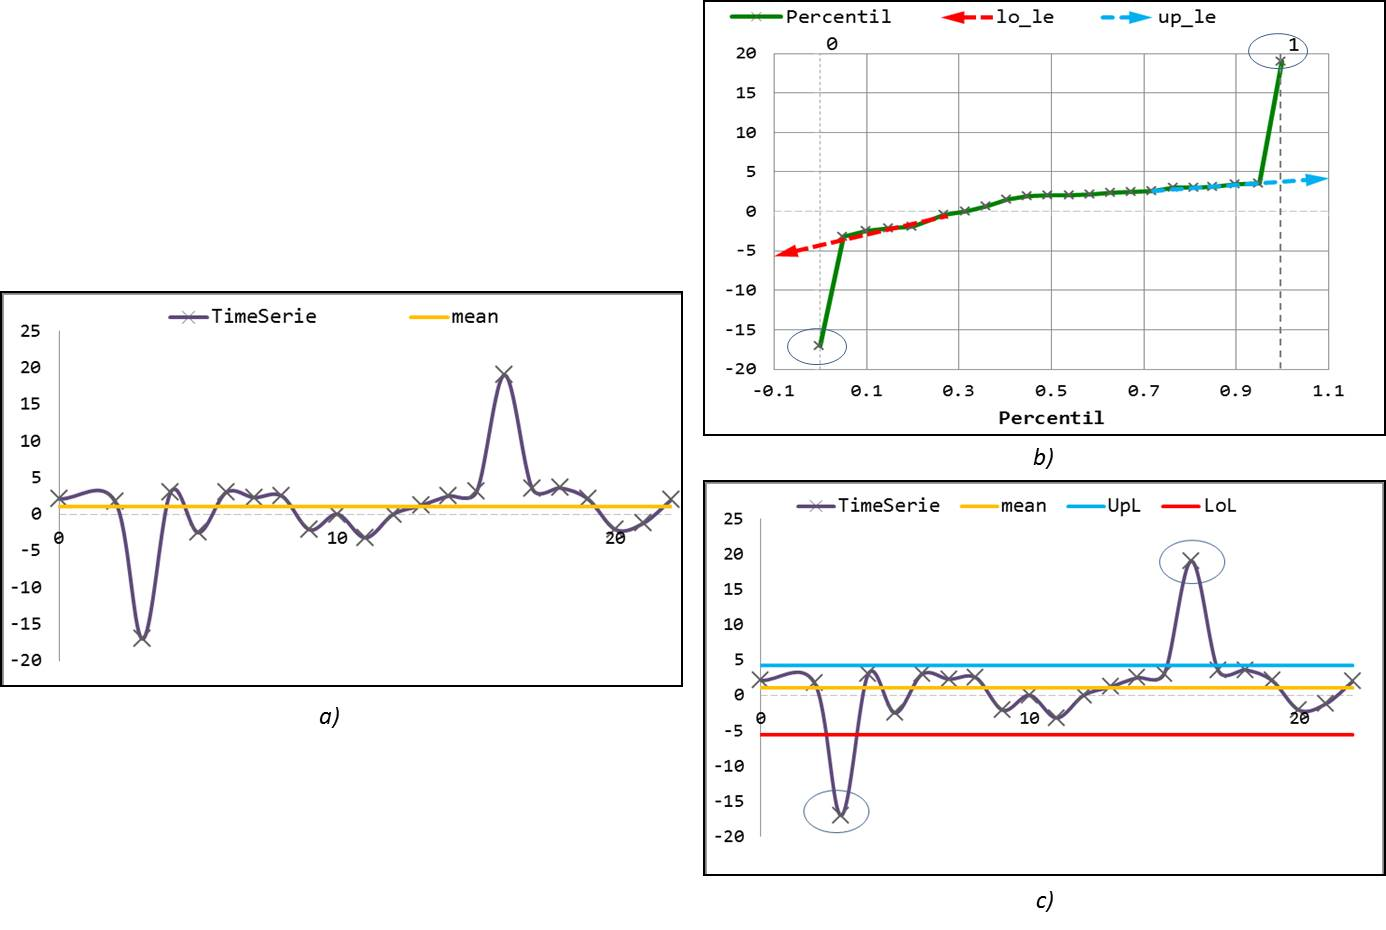
\includegraphics[scale=0.5]{Figures/percentil_example.jpg}
  \caption{\textit{a)} Simple time series, similar to Figure \ref{fig:six_sigma}. \textit{b)} Percentile curve of the time series. Trends \textit{lo\_le} and \textit{up\_le} are the linear regression of the extreme percentile values.  \textit{c)}
The percentile analysis approach detects two outlier values (in the ellipse), these values do not belong to the interval  
$[LoL, UpL]$.}
  \label{fig:percentile}
\end{figure}

In contrast to the six sigma approach, note that percentile analysis does not have symmetric limits to the mean. Observe how the $UpL$ and $LoL$ are not symmetric to the mean $\mu$ in figure \ref{fig:percentile}{\color{red} .\textit{c)}}. This property allows the use of this approach for distributions that are not necessarily Gaussian.


\begin{figure}[h!]
  \vspace{0.5em} %better style
  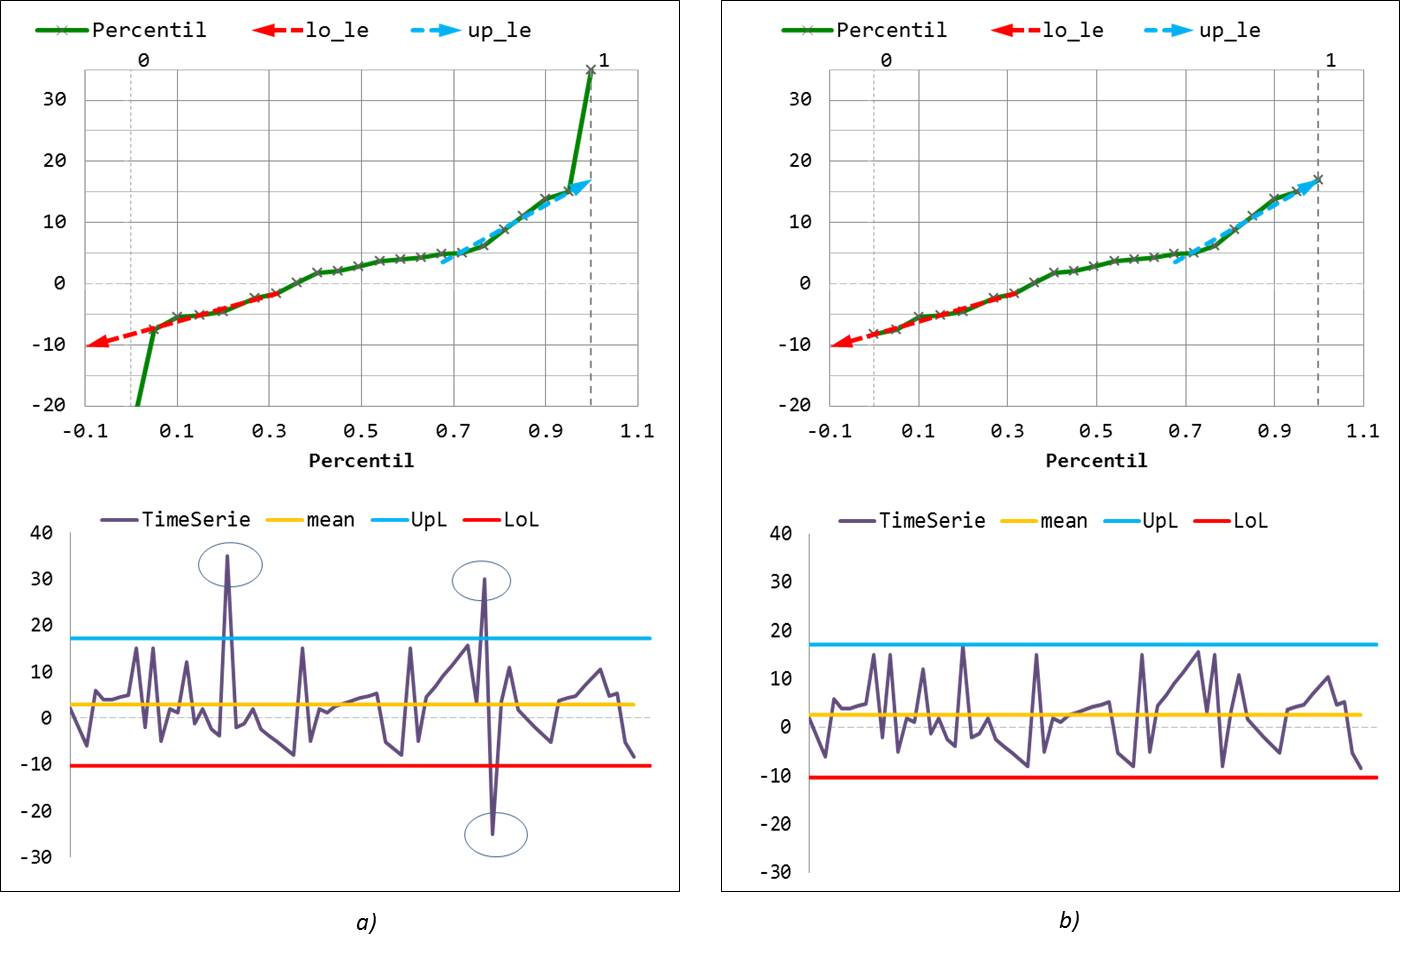
\includegraphics[scale=0.5]{Figures/percentil_example_2.jpg}
  \caption{\textit{a)} Three outliers detected using the percentile analysis approach. \textit{b)} The same time series presented without the three detected outliers.}  
  \label{fig:percentile2}
\end{figure}

To exemplify the behavior of the percentile analysis, observe Figure \ref{fig:percentile2} where any value outside the interval $[LoL, UpL]$ is detected as outlier. 

\subsubsection{Comparison between six sigma and percentile analysis}
To evaluate both approaches, we perform several experiments \footnote{The complete set of experiments are included as digital annex in \textit{/Thesis\_project/iPythonBooks/Outlier\_detection}} over theoretical signals where we define the limits of the variable. The random variable is defined by $2A \cdot$ $np.random.rand(n,1)$ $- A$ \footnote{Create an array of the given shape and populate it with random samples from a uniform distribution over [0, 1)}, therefore the variable is limited in the range $[-A, A]$. We introduce outliers on purpose, to know if both approaches detect these outliers. Figure \ref{fig:comparison} shows in \textbf{a)} the random signal in range [-10, 10] with added outilers, and \textbf{b)} the detection of outliers by using both approaches.    


\begin{figure}[h!]
  \vspace{0.5em} %better style
  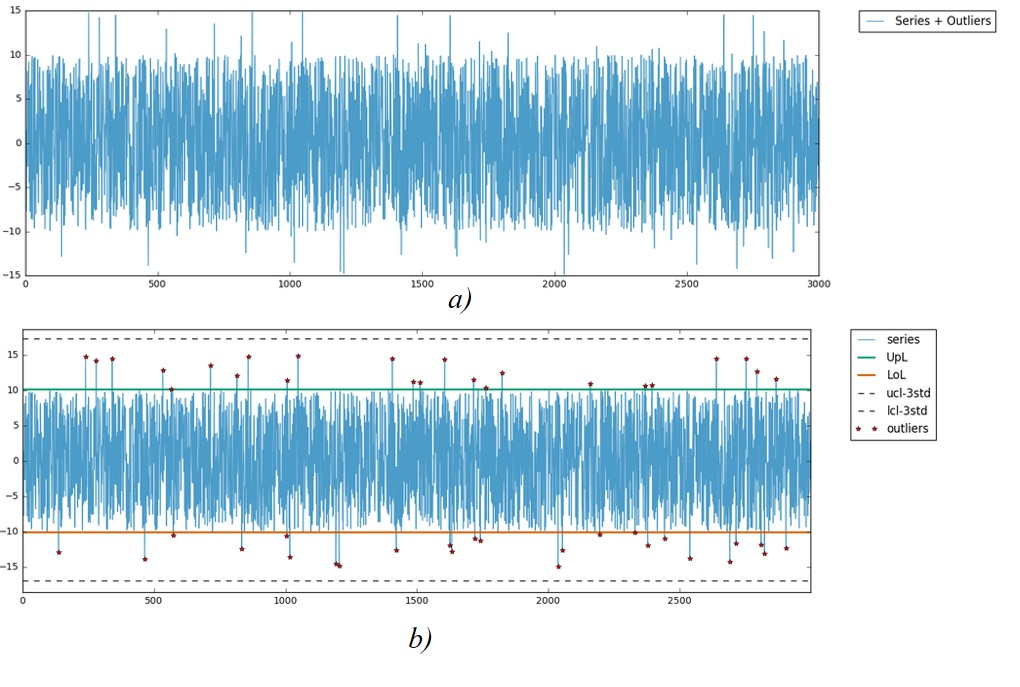
\includegraphics[scale=0.5]{Figures/test.jpg}
  \caption{\textit{a)}A random signal with range of [-10, 10] with added outliers.  \textit{b)} Detection of outliers by using six sigma and percentile analysis approach.}  
  \label{fig:comparison}
\end{figure}

One observe how the limits of the six sigma approach (i.e. ucl-3std and lcl-3std) do not detect any outlier (i.e. $0\%$) while the percentile approach detects 100\% of them. In the following experiment in figure \ref{fig:test2},we tested the quantity of outliers that this approach can detect with an accuracy greater than 95\%. We include the results of six sigma approach to make comparison between the two approaches. The tested time series has length of 3000, and one observes the detection precision  decreases less than 95\% when the original time series contains more than 300 inserted outliers.

  
\begin{figure}[h!]
  \vspace{0.5em} %better style
  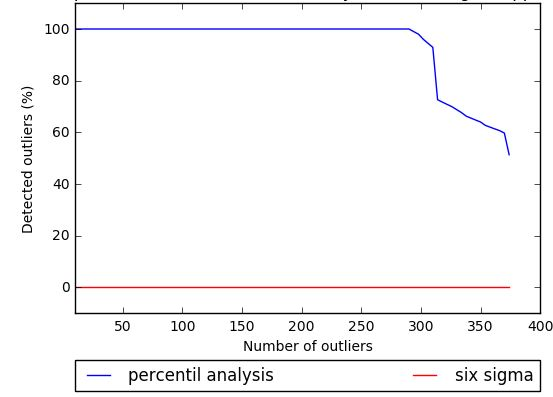
\includegraphics[scale=0.5]{Figures/test2.jpg}
  \caption{Testing the number of outliers that percentile analysis and six sigma approach can detect.}  
  \label{fig:test2}
\end{figure}

This happens because the extreme values begin to represent more than 10\% of the total points of the series. Are these points part of the process?. Figure \ref{fig:test3} shows this situation. 

\begin{figure}[h!]
  \vspace{0.5em} %better style
  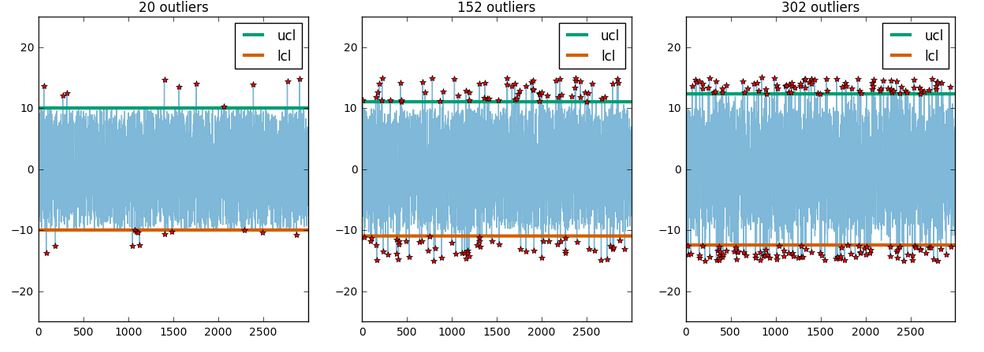
\includegraphics[scale=0.5]{Figures/test3.jpg}
  \caption{Percentile analysis approach spotting outliers.}  
  \label{fig:test3}
\end{figure}

We use the percentile analysis to depurate the time series from values that do not correspond to the underlying process of the variable. This is important because outlier values could create havoc in the training process, visualization of results and other further steps. For example, the non convergence of the tuning parameters of the model during the training process. \footnote{We save the detected values of this approach in collection: \textit{detection outlier}. Script: \textit{1. detection\_using\_quartiles.py}}. The six sigma approach is used as well when we apply the SAX process according to section \ref{comparison_sax_hmm}. Table \ref{tab:six_perc} shows the number of points that were detected as outliers for a set of variables. One observes that each approach has different results for each particular variable. We observe that the percentile analysis approach has best detected outliers, since there is no assumption of a Gaussian distribution of the time series as \textit{six-sigma} does.       


\begin{table}[]
\centering
\caption{Number of points (individual measurements) spotted as outliers.}
\label{tab:six_perc}
\tiny
\begin{tabular}{l|l|l|}
\cline{2-3}
                                                 & \multicolumn{2}{c|}{Number of detected points} \\ \hline
\multicolumn{1}{|l|}{Variable}                   & \# Percentil Analysis      & \# Six Sigma      \\ \hline
\multicolumn{1}{|l|}{V004\_vent01\_hum\_out}     & 148                        & 362               \\ \hline
\multicolumn{1}{|l|}{V023\_vent02\_temp\_out}    & 105                        & 279               \\ \hline
\multicolumn{1}{|l|}{V005\_vent01\_CO2}          & 114                        & 473               \\ \hline
\multicolumn{1}{|l|}{V022\_vent02\_CO2}          & 141                        & 474               \\ \hline
\multicolumn{1}{|l|}{V006\_vent01\_temp\_out}    & 87                         & 264               \\ \hline
\multicolumn{1}{|l|}{V012\_vent01\_temp\_in}     & 294                        & 531               \\ \hline
\multicolumn{1}{|l|}{V021\_vent02\_hum\_out}     & 193                        & 403               \\ \hline
\multicolumn{1}{|l|}{V029\_vent02\_temp\_in}     & 324                        & 604               \\ \hline
\multicolumn{1}{|l|}{V037\_tabs\_cold\_SW}       & 87                         & 152               \\ \hline
\multicolumn{1}{|l|}{V074\_tabs\_warm\_NO}       & 310                        & 280               \\ \hline
\multicolumn{1}{|l|}{V075\_tabs\_cold\_NO}       & 164                        & 132               \\ \hline
\multicolumn{1}{|l|}{V099\_blinds\_height\_N\_o} & 35                         & 13                \\ \hline
\multicolumn{1}{|l|}{V102\_blinds\_height\_N\_i} & 33                         & 13                \\ \hline
\multicolumn{1}{|l|}{V105\_blinds\_height\_O\_o} & 54                         & 17                \\ \hline
\multicolumn{1}{|l|}{V108\_blinds\_height\_O\_i} & 34                         & 12                \\ \hline
\multicolumn{1}{|l|}{V111\_blinds\_height\_S\_o} & 48                         & 16                \\ \hline
\multicolumn{1}{|l|}{V112\_blinds\_angle\_S\_o}  & 30                         & 12                \\ \hline
\multicolumn{1}{|l|}{V114\_blinds\_height\_S\_i} & 50                         & 14                \\ \hline
\multicolumn{1}{|l|}{V115\_blinds\_angle\_S\_i}  & 35                         & 10                \\ \hline
\multicolumn{1}{|l|}{V117\_blinds\_height\_W\_o} & 26                         & 11                \\ \hline
\multicolumn{1}{|l|}{V118\_blinds\_angle\_W\_o}  & 25                         & 11                \\ \hline
\multicolumn{1}{|l|}{V120\_blinds\_height\_W\_i} & 38                         & 12                \\ \hline
\multicolumn{1}{|l|}{V121\_blinds\_angle\_W\_i}  & 39                         & 11                \\ \hline
\end{tabular}
\end{table}




\section{Feature Selection}
\label{sec:feature_selection}

This module assists the selection of features for the creation of multivariate samples as it was explained in section \ref{sec:MVA}. We want to choose the best features from different variables such that one sample can express information in a more high level, making more robust and integral our proposed models. This is the approach of the \textit{GaHMM seasonal} model that is explained in section \ref{sec:seasonal_model}. One common approach to feature selection is the use of the Kullback–Leibler distance, this approach allows the measure of information when one uses an arbitrary feature. We borrowed and adapted the concepts that are presented in (\citeauthor{eguchi2006interpreting}, 2006) \cite{eguchi2006interpreting} to explain the feature selection that was performed in this study. If we let $P$ and $Q$ be two probability distributions of one feature $x$ over two different clusters of data. Then let $p(x)$ and $q(x)$ be their respective probability functions. The Kullback–Leibler distance is thus defined by:

\begin{equation}
D(P,Q) = \int p(x) log 	\dfrac{p(x)}{q(x)} dx
\end{equation}

Two basic properties of D can be observed from this formula: 
\begin{itemize}
\item[a.] non-negativity $D(Q,P) \geq 0$, and a especial case: if $P == Q$ then $D(Q,P)=0$
\item[b.] asymmetry $D(P,Q) \neq D(Q,P)$
\end{itemize}
Since this distance is asymmetry, it is normal practice to use the symmetric K–L distance (also known as J-distance) \cite{coetzee2005correcting}: 

\begin{equation}
J(p,q) = D(p,q) + D(q,p)
\label{J_distance}
\end{equation}

It follows then, that if $J(p,q) = 0$ the two clusters characterized by the feature $x$ are similar. Stated in another way, the two clusters should be a single cluster (or a feature $x$ does not provide
any information helpful to the discrimination of these two groups
). In contrast, if $J(p,q)$ is high then surely the feature $x$ describes two different clusters. Thus, one is interested in finding the features that return a high J value on latent clusters. This selection can be done by sophisticated and robust methods (\citeauthor{sui2013information}, 2013 \cite{sui2013information}). However, this work uses a simplified version for feature
selection, since we are only interested in having an approximate ranking of features, due to the evaluation process for GaHMM scoring the clustering quality of each model, so then we can be sure that the feature selection was good. The final objective of our proposition \footnote{Script \textit{2.entropy\_calculation.py} implements this proposition.} is a collection of JSON documents where one can rank the
features from the highest "gain of information" until the lowest one. This ranked list of feature is created by the following steps (see figure \ref{fig:schema} to illustrate the process):   

\begin{itemize}
\item[1] Features are calculated in a daily fashion using the script \textit{2.statistics daily.py}. The feature data space (i.e. daily feature collection) is created according to the feature list in annex \ref{tab:feature_list}.
\item[2] Random groups of data in the feature space are created. In our case, 7 groups of data were created by using the weekday name label \footnote{This choice is arbitrary. It was done because we observed that variables like $CO_2$, temperature and others change between working days and weekends. Therefore it was considered convenient to create the random clusters by using the names of the day. Other ways to create random groups can also be done.}.
\item[3] Chose one feature from the feature list and perform the K-L distance $J(p,q)$ over all the created groups in a pairwise fashion. Save the best K-L distance into the JSON document collection \textit{'feature selection'}.
\item[4] Order features according to the best J value. (i.e. ranked list).   
\end{itemize}

\begin{figure}[h!]
  \vspace{0.5em} %better style
  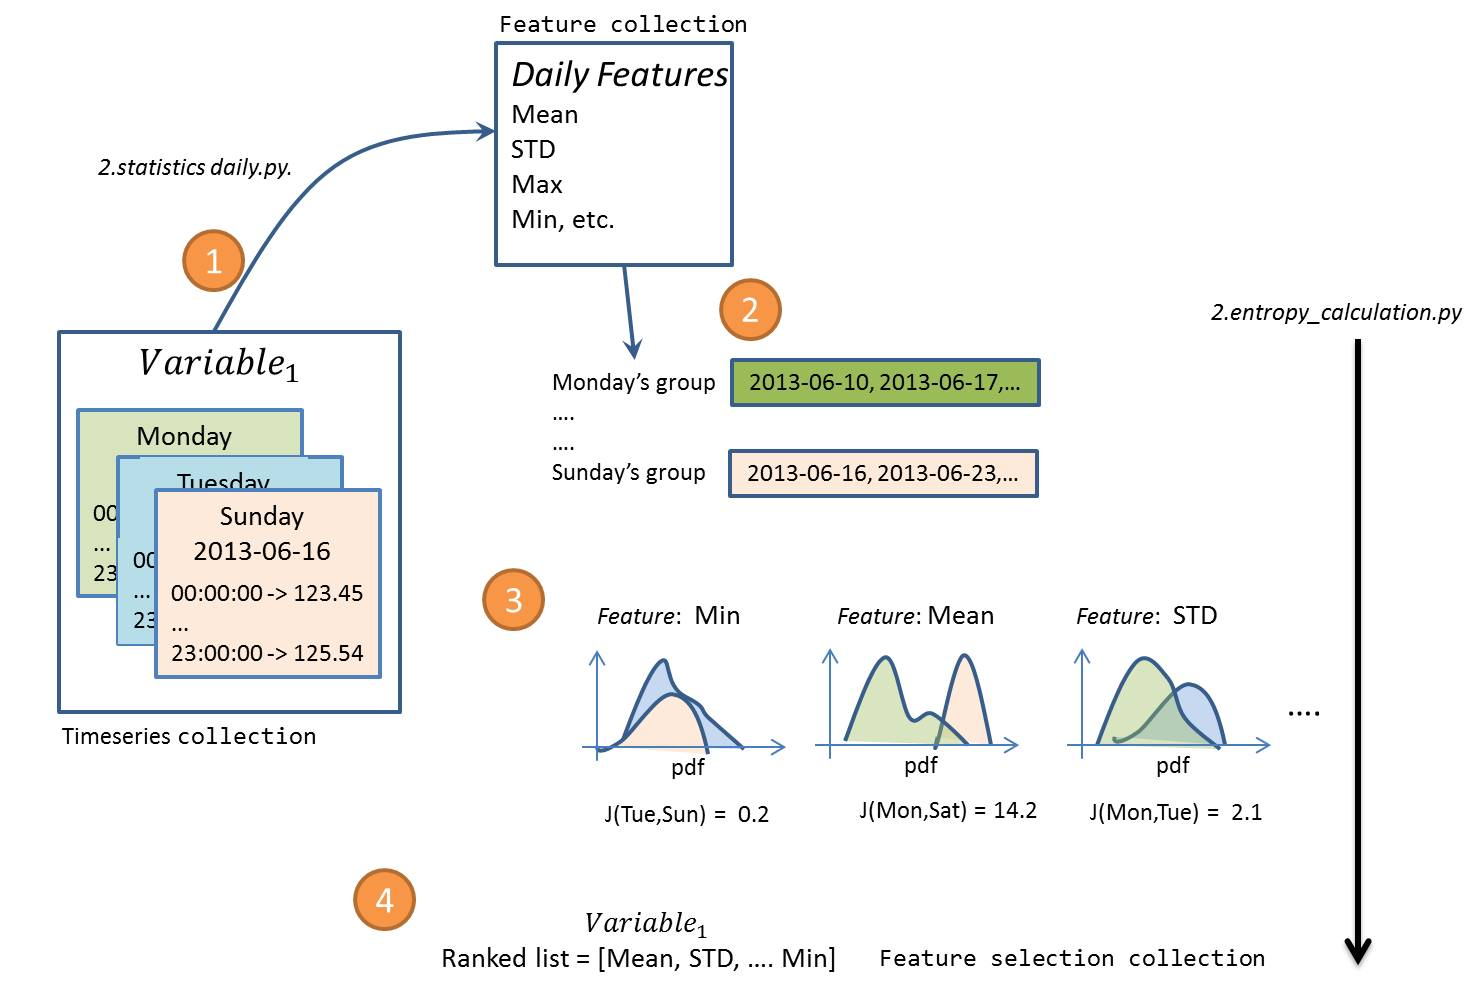
\includegraphics[scale=0.5]{Figures/feature_selection.jpg}
  \caption{Schema of the implemented feature selection}
  \label{fig:schema}
\end{figure}


By always conserving the same random groups for each interaction, it is possible to measure (approximately) the gain of information that each feature provides. Other analyses like the correlation between features can be done \cite{sui2013information}, but this is outside of the scope of this study. One can see that each variable (e.g. $CO_2$, humidity, temperature, etc.) has its own ranked list (i.e. some features that are important for a set of variable $V_1$, are less important for another set of variable $V_2$). Since we keep an invariable definition of the random groups, at the end, one can obtain a ranking of the features according his respective gain of information.


\subsubsection{Ripple Factor}
\label{sec:ripple}

We calculate 18 features in daily fashion for each variable, the complete list of features are in annex \ref{tab:feature_list}. We propose one feature that help us to gain information for the seasonal model explained in section \ref{sec:seasonal_model}. Here, we explain its concept: Given a time series of length $N$, a new feature called ripple factor captures the shape of the trend that crosses the mean $\mu_x$ of the series. The feature has three key values to converge: 
\begin{itemize}
\item[a)] The feature converges to 1 when at most points of the time series are above the mean.
\item[b)] The feature converges to 0, crossing the mean on many occasions. 
\item[c)] The feature converges to -1 when most of the point of the time series are below the mean.
\end{itemize}

This behavior is shown in figure \ref{fig:rf_ex1}. To achieve the previous description, we use a common ratio (i.e. 1/N) for all the points that belong to the series, and create a power series that maps the position of each series point $\textbf{p}$ to the exponent of each term according to the condition $\mathscr{C}_f$. In this way, all the points that are above the mean are used to form the term $A_b$ and the rest of the points are used for the term $B_e$. Finally, the difference between these two terms divided by the size of the series is the mathematical definition of our feature. The condition $\mathscr{C}_f$, the range and mathematical definition of the proposed feature are specified in equation \ref{ripple_factor}.    

\begin{figure}[h!]
  \vspace{0.5em} %better style
  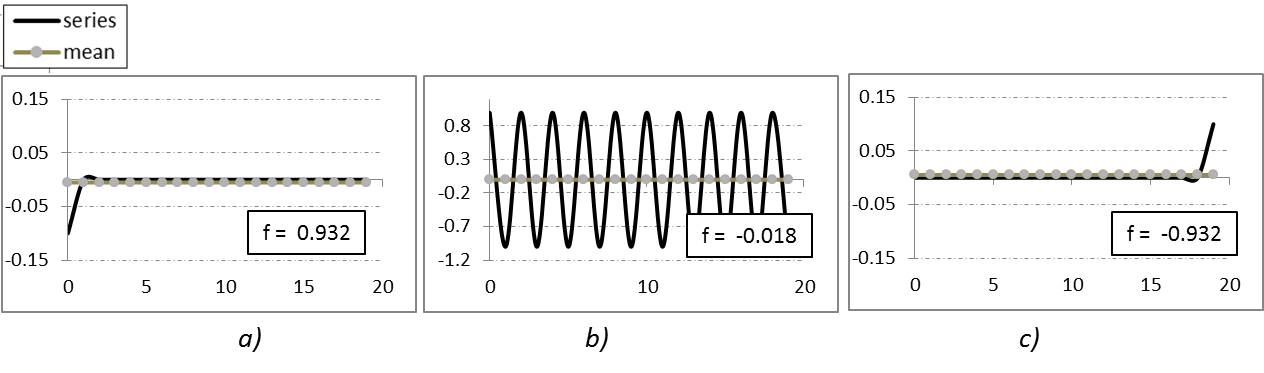
\includegraphics[scale=0.7]{Figures/Example_1_rf.jpg}
  \caption{Behavior of Ripple Factor feature}
  \label{fig:rf_ex1}
\end{figure}


\begin{equation}
\begin{array}{lcl}
\text{Time serie}			&:& X(n) = [x_0, x_1, x_2, ..., x_p], \quad |X| = N \\ \\
\text{Feature range} 		&:& \mathscr{R}_f \{ {X(n)}\} \in (-1, 1), \quad 
								\mathscr{R}_f \{ {X(n)}\} \in \mathbb{R}^+ \\ \\
\text{Feature condition}	&:& \mathscr{C}_f \{ {X}\} = \begin{cases}  
				A_b = \mathlarger{\sum_{x_p >= \mu_x} 2^{\ p \frac{1}{N}}}, & \forall p \in [0,N-1] \\ \\  											B_e = \mathlarger{\sum_{x_p < \mu_x} 2^{\ p  \frac{1}{N}}}, & \forall p \in [0,N-1] 			
							\end{cases} \\ \\
\text{Feature definition}	&:& \mathscr{R}_f \{ {y(n)}\} = ln(2) \cdot \dfrac{A_b - B_e }{N}  							
\end{array}
\label{ripple_factor}
\end{equation}

The limits of this feature are found when either $A_b$ or $B_e$ is equal to zero (but not simultaneously). For the upper limit, this occurs when all the points are above or equal to the mean. Figure \ref{fig:ripple_limits} shows how the limits behave according to the size of the series. Furthermore, we show in equation \ref{limit_cal} the upper and lower limit of this feature.

\begin{figure}[h!]
  \vspace{0.5em} %better style
  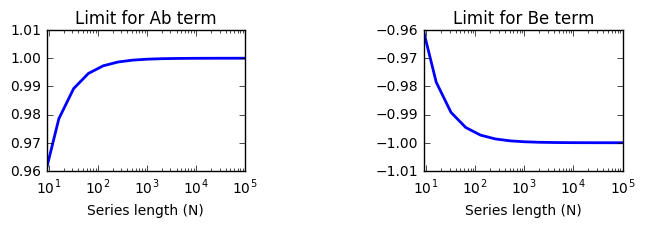
\includegraphics[scale=0.8]{Figures/limits_ripple_feature.jpg}
  \caption{Limits for the Ripple Factor feature according to the length of the time series.}
  \label{fig:ripple_limits}
\end{figure}


\begin{equation}
\begin{array}{lcl}
\text{Upper limit when $B_e = 0$} &:& \mathlarger{\lim_{N\to\infty} ln(2) \cdot \dfrac{A_b - B_e }{N} 
                                = ln(2) \cdot \lim_{N\to\infty} \dfrac{ \mathlarger{\sum_{p=0}^{N-1} \ 2^{\ p \frac{1}{N}} }}{N}}\\ \\
                              &:& \mathlarger{ ln(2) \cdot \lim_{N\to\infty} \dfrac{1}{ N (2^{\ \frac{1}{N}}-1)} = 1 }  \\ 	
                              
\text{Lower limit when $A_b = 0$} &:& \mathlarger{\lim_{N\to\infty} ln(2) \cdot \dfrac{A_b - B_e }{N} 
                                = -ln(2) \cdot \lim_{N\to\infty} \dfrac{ \mathlarger{-\sum_{p=0}^{N-1} \ 2^{\ p \frac{1}{N}} }}{N}}\\ \\
                              &:& \mathlarger{-ln(2) \cdot \lim_{N\to\infty} \dfrac{1}{ N (2^{\ \frac{1}{N}}-1)} = -1 } 						
\end{array}
\label{limit_cal}
\end{equation}

The following part discusses several examples that use this feature. We propose comparable examples where the mean is equal to zero in all the cases. The capacity of the ripple factor to discriminate time series that have similar statistics is appreciated in figure \ref{fig:rf_ex2}. The three time series have the same mean, variance, percentiles, and maximum and minimum value, but the ripple factor for each one is different, so that, we can discriminate for example a sine signal from a cosine signal. 

\begin{figure}[h!]
  \vspace{0.5em} %better style
  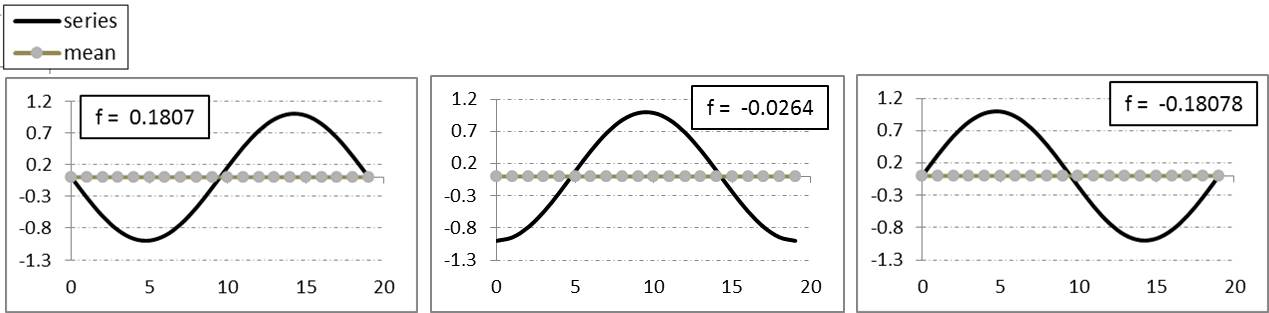
\includegraphics[scale=0.7]{Figures/Example_2_rf.jpg}
  \caption{Ripple factor for sine and cosine signal.}
  \label{fig:rf_ex2}
\end{figure}

In figure \ref{fig:rf_ex3}, we appreciate how this feature changes depending on the shape of each particular signal. The examples show how this feature changes as soon as the oscillations approach the mean. The closer the oscillations are to the mean, the nearer to zero the feature is. \\

\begin{figure}[h!]
  \vspace{0.5em} %better style
  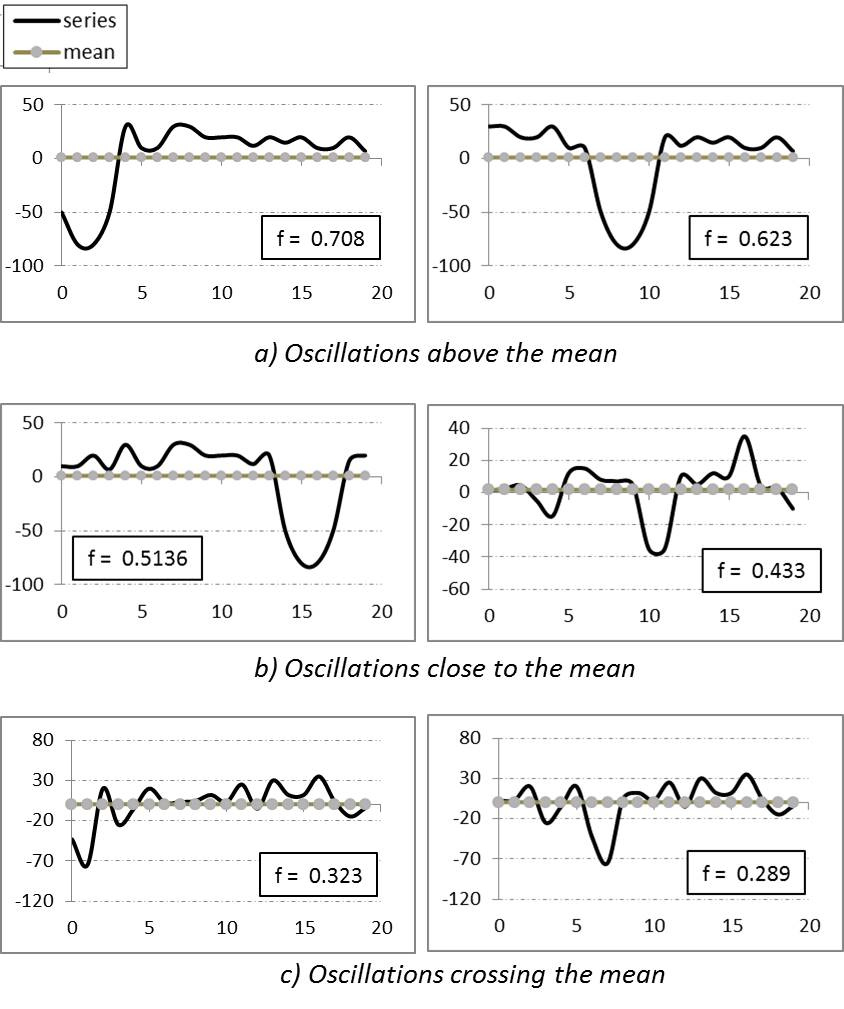
\includegraphics[scale=0.7]{Figures/Example_3_rf.jpg}
  \caption{Ripple factor for sine and cosine final.}
  \label{fig:rf_ex3}
\end{figure}


\textit{Extension of the ripple factor feature:} \\

The last behavior explained in figure \ref{fig:rf_ex3} allows to extend the concept of the ripple factor to one that is most general. If we change the definition of the feature condition $\mathscr{C}_f$, we can substitute the parameter of comparison (in the original definition $\mu_x$) for any other numeric value $v \in \mathbb{R}$. This change is useful when for some reason we need to know whether or not most of the
oscillations are close to the value $v$ \\


\textit{Discussion of the Ripple Factor:} \\
 
As we see in figure \ref{fig:ripple_limits} the feature is sensitive to the length of the series. Nevertheless, for this study the feature was calculated using a fixed window of one day (i.e. sub-sequences of same size), therefore the limits are well defined. To know how much these limits differ, we consider a time series of size $N=10$ and one of size $N=50$. Their limits are $0.965$ and $0.993$ respectively and the difference is only 0.028. To know whether this difference is significant, an evaluation must be done. The mentioned evaluation goes beyond the purposes of this study and we only use this feature because the length of sub-sequences is fixed (therefore the limits are well defined) and because using the Kullback–Leibler divergence, this feature obtains a good gain of information being selected for the \textit{GaHMM-seasonal} profile, explained in section \ref{sec:seasonal_model}. \\

Another relevant aspect of this feature is the fact that it does not depend on the amplitude of the treated signal. This fact allows the signal to be amplified or reduced without changing the ripple factor. This can be an advantage when the shape of the series is an important characteristic to analyze. Finally, this feature is complementary to other statistics such as the the mean, standard deviation and others, but not a substitute for them.




\section{GaHMM Modeling}
\label{modeling}

Hmmlearn \cite{gahmm_manual} \footnote{\url{http://hmmlearn.readthedocs.io/en/stable/}} is the python library used in this project. We use the internal methods that this library offers in order to perform the training process. We recall here the training process that was explained in section \ref{sec:problems}, and we add information about the employed library. 


\begin{itemize}
\item Learning/ training process: The HMM model is fitted with the observed samples $\mathbb{O} = (O_1, O_T)$. The definition of the observed samples is very important since it defines the kind of HMM to use. Each proposed model define the samples according to the underlying problem that each model wants to solve. In all the cases we use a \textit{GaHMM} model since we use sequential continuous values. The definition of the observed samples are explained in each model. The library method to use for the training process is called: \textbf{fit} method \cite{gahmm_manual}, this implements the solution that was explained in section \ref{sec:learning_HMM}.
\item Evaluation process: For evaluation purposes, the log probability of $P(\mathbb{O} |\mathbb{S}, \lambda)$ (i.e. equation \ref{independence_ass}) is used to select the best trained model. The model that fits the best the parameters of $\lambda$ is the one who has the greatest probability. The library method that calculates $P(\mathbb{O} |\mathbb{S}, \lambda)$ is the \textbf{score} method using the forward/backward algorithm (section \ref{sec:evaluation_HMM}).    
\item Decoding process: When one obtain the best model, there is a perfect matching between the observed samples $\mathbb{O}$ and the sequences of states $\mathbb{S}$. One says that each hidden state $S_k$ emits one sample $O_i$. To know the likely sequence of hidden states the \textbf{predict} method solves the decoding problem by using Viterbi algorithm. (section \ref{sec:decoding_HMM}).  
\end{itemize}

\subsection{GaHMM Training process}
\label{sec:training_process}
 
The training process is done by solving the HMM evaluation problem (section \ref{sec:evaluation_HMM}). This evaluation is done by the \textit{score} method \cite{gahmm_manual}, where the log probability of $p(\mathbb{O}|\lambda)$ is calculated. The log probability has practical advantages, and is useful for finding the best trained model. This work adopts the use of the log probability of $p(\mathbb{O}|\lambda)$ for finding the best model. However, since its value is not easy to understand, this document reports probability in the interval of [0,1]. For this purpose, given that each observation could have been drawn by each every hidden state with a certain probability, this allows us to perform a time-dependent clustering task \citep{pfundstein2011hidden}. In this way, given the observed sequence $\mathbb{O} = (O_1, O_2,... O_T)$ and the correspondent sequence of hidden states $\mathbb{S} = (S_1, S_2,..., S_T)$ \footnote{Recall: There are $K$ hidden states for a HMM, therefore $\mathbb{S}$ is a permutation of $K$ values with length equal to $T$}, we calculate the average of $p(\mathbb{O}|\mathbb{S})$ as follows:

\begin{equation}
\overline{p}(\mathbb{O}|\mathbb{S}) = \dfrac{1}{T} \sum_{i=1}^{T} p(O_i | S_i)
\label{ec:average_probabilty}
\end{equation}

Where $T$ is the total number of observations, $S_i$ is the likely hidden state that emits the observation $O_i$, and $ p(O_i | S_i) \in [0,1]$ is the probability that the observed sample $O_i$ was emitted by the hidden state $S_i$. The hidden state sequence $\mathbb{S}$ that matches with the observed sequence is found by the \textbf{predict} method \cite{gahmm_manual} of the GaHMM library. It follows that the bigger the log probability is, the better the average $p(\mathbb{O}|\mathbb{S})$ is. Therefore, the equation \ref{ec:average_probabilty} shows a direct relationship with the log probability and his range is in the interval of [0,1].This is the way in which we will report
the results throughout the document.

    
\subsubsection{Cross validation process}
\label{sec:cross}

As is explained in section \ref{sec:learning_HMM}, the EM algorithm is a gradient-based optimization method that can be stuck in local optima. Hence, it is generally recommended to run several instances of the model with various initialization values, and then choose the best one. This process of training leads to problems of over-fitting in some cases. To avoid this, and to guarantee a well-trained model, the cross-validation technique is performed in most of the cases. Since our proposition deals with time series, the k-fold cross-validation technique is
not necessarily valid if we do not consider the time correspondence (\citeauthor{bergmeir2015note}, 2015) \cite{bergmeir2015note}. The traditional k-fold cross validation performs a random partitioning of the original sequence into k equal sized blocks. One inconvenient is that the samples are treated as independent sequences and not as a part of a sequence of events. Fitting the HMM with a random order of samples $O_i$ causes a poor performance of the model. Our proposed approach for cross-validation follows the indications of \citeauthor{bergmeir2015note}'s work, therefore the random selection is avoided. In short, the partial observed sequences for training $\mathbb{O}_{train}$ and testing $\mathbb{O}_{testing}$ respect the original order of the time series. Figure \ref{fig:k-fold} shows the schema for k-fold cross validation of $k=5$. 


\begin{figure}[h!]
  \vspace{0.5em} %better style
  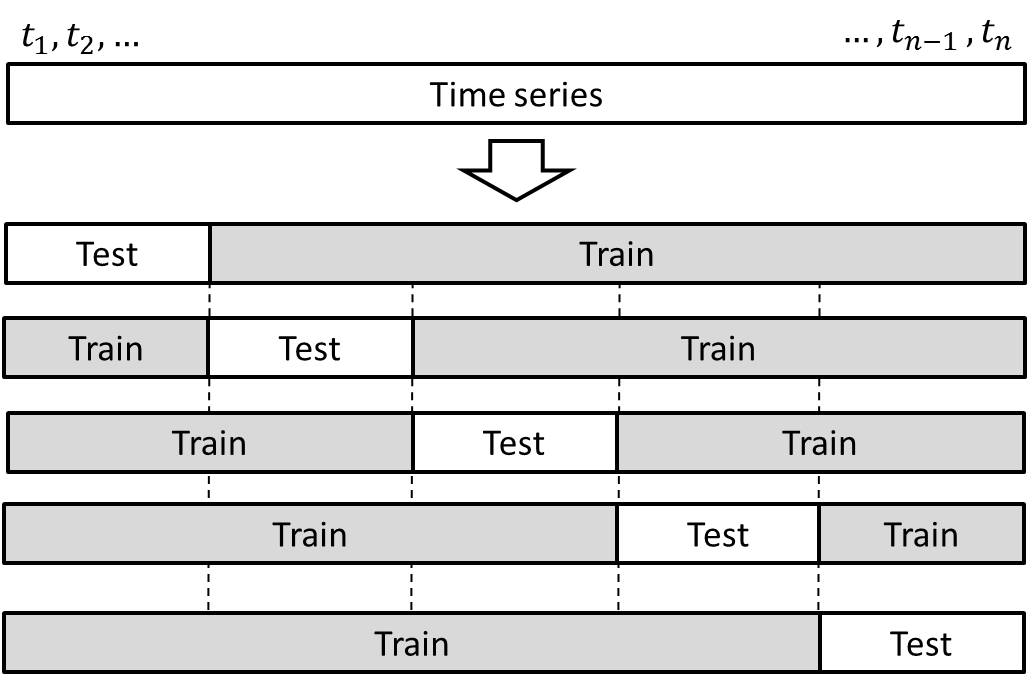
\includegraphics[scale=0.45]{Figures/k-fold.jpg}
  \caption{k-fold cross validation with $k=5$. Note that the order of the time series is not altered, no random selection is done.}
  \label{fig:k-fold}
\end{figure}


\subsubsection{Fixing parameters of GaHMM and cross validation process}

Fortunately, the GaHMM library  \cite{gahmm_manual} proposes some parameters by default. Since the Gaussian Model implements a monitor routine for checking the internal convergence, there was no need to change the default parameters for: \textit{min\_covar, means\_prior, means\_weight, n\_iter, tol}. Nevertheless, in order to guarantee the convergence of the trained model, each hidden state uses a diagonal covariance matrix (i.e. \textit{covariance\_type= "diag"}). Additionally, as it was explained in section \ref{sec:evaluation_HMM}, Viterbi algorithm was chosen by default. The only parameter that was modified for each training round was the number of components, which is the number of hidden states to use (i.e. \textit{n\_components} parameter). Regarding the cross validation process, we found by doing experiments that select $k$ in the interval of [10, 15] is a good choice. If $k < 10$, the final clusters tend to be mixed, while $k > 20$, the over-fitting effect is evident.  


\paragraph{Scripts for training}
Two python scripts were created for training the three different models explained in section \ref{implemented}. Table \ref{scripts_impl} presents the context were each script is used. Details about the models are in the next section, here the structure of each training script is explained.  

Both training scripts vary the \textit{n\_components} parameter in an interval of $[n_{min}, n_{max}]$, in which $n\_components = n$ the k-fold cross validation process is executed, afterwards the best model is chosen (for us, this is called a round). At the end, the best model $M_j$ among all the rounds is picked as the final model. This process is explained in the following pseudo-codes:


\begin{table}[]
\centering
\scriptsize
\caption{Implemented scripts for training}
\label{scripts_impl}
\begin{tabular}{|l|l|l|}
\hline
\textbf{GaHMM model} & \textbf{Script}                           & \textbf{Observed sample type}                              \\ \hline
Profile              & 4.hmm\_learning\_per\_variable\_k-fold.py & Univariate sample (daily profile of the selected variable) \\ \hline
Seasonal             & 4.hmm\_learning\_k-fold.py                & Multivariate sample (features of several variables)        \\ \hline
Interactional        & 4.hmm\_learning\_k-fold.py                & Multivariate sample (linear correlation between variables) \\ \hline
\end{tabular}
\end{table}


\begin{figure}[h!]
  \vspace{0.5em} %better style
  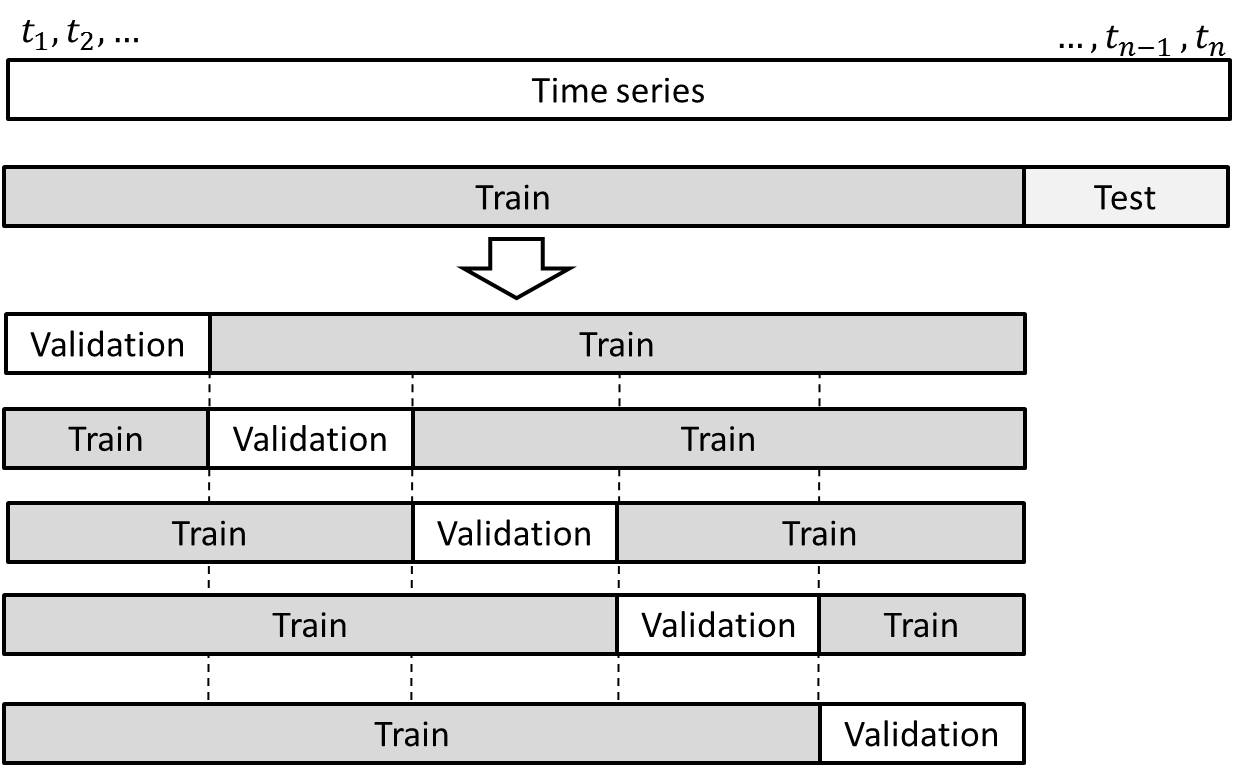
\includegraphics[scale=0.45]{Figures/k-fold-1.jpg}
  \caption{k-fold cross-validation with $k=5$ for a \textit{GaHMM} model. The testing
set is separated to be used at the end of the k-fold cross validation process (Script: \textit{4.hmm\_learning\_k-fold.py}).}
  \label{fig:k-fold-1}
\end{figure}

Pseudo-code for script \textit{4.hmm\_learning\_k-fold.py}:  

\begin{itemize}
\item[1] Extract information from the \textit{metadata} collection for the running of the corresponding training process. (i.e. variables, categories, daily vector to use, etc.)
\item[2] Establish the timeline to work with, the training set and the testing set \footnote{The testing set differs from the validation set. The testing set is a reserved part of the whole data that is used
just at the end of the whole training process. Its purpose is to test if the trained model is capable also of working on data that it has not seen before}. Here the observed sequence $\mathbb{O}$ is defined.  
\item[3] Define the minimum and maximum number of hidden states for the training process. $n \in [n_{min}, n_{max}]$. Initialize $n= n_{min}$.
\item[4] Initialize a Gaussian Hidden Markov model with $n\_components = n$.
\item[5] Perform the k-fold cross-validation over the training data set, see figure \ref{fig:k-fold-1}. At each step of the cross-validation process, the best \textit{GaHMM} model ($M_i$) is chosen by using the validation set \footnote{For this purpose, the log probability of $p(\mathbb{O}|\lambda)$ of the trained model is used.}. 
\item[6] Test the best model ($M_i$) that was found in the k-fold cross-validation process using the test set. Compare the current model ($M_i$) with the last best model ($M_j$) and elect the best model \footnote{$M_j$ is the best model to have been found among all the rounds. When $n=n_{min}$ then $M_j = M_i$. }.
\item[7] Increase the number of hidden states $n = n+1$. If $n<n_{max}$ then go to step 4, otherwise the training process is finished.  
\end{itemize}  


\begin{figure}[h!]
  \vspace{0.5em} %better style
  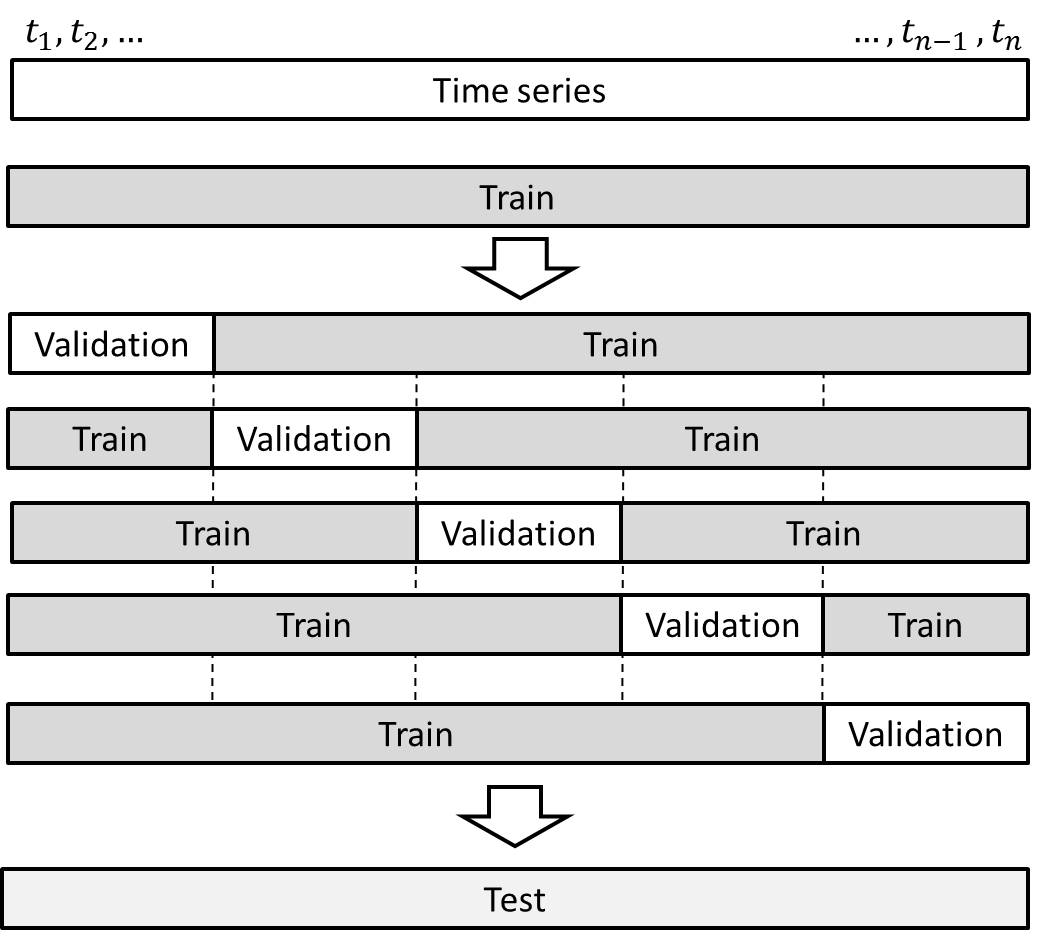
\includegraphics[scale=0.45]{Figures/k-fold-2.jpg}
  \caption{k-fold cross validation with $k=5$ for a \textit{GaHMM} model. The testing set is the entire time series. This allows the verification of the fitness of the model across the
entire time series (Script: \textit{4.hmm\_learning\_per\_variable\_k-fold.py}).}
  \label{fig:k-fold-2}
\end{figure}

Here the pseudo-code for script \textit{ 4.hmm\_learning\_per\_variable\_k-fold}: 

\begin{itemize}
\item[1] Extract information from the \textit{metadata} collection for running the correspondent training process. (i.e. variables, categories, daily vector to use, etc.)
\item[2] Establish the timeline to work with, and the training set \footnote{Since we are interested in finding all possible daily patterns across multiple years, at the end of the cross validation process, we test each model with all the available data.}. Here the observed sequence $\mathbb{O}$ is defined.   
\item[3] Define the minimum and maximum number of hidden states for the training process. $n \in [n_{min}, n_{max}]$. Initialize $n= n_{min}$.
\item[4] Initialize a Gaussian Hidden Markov model with $n\_components = n$.
\item[5] Perform the k-fold cross-validation over the training data set, see figure \ref{fig:k-fold-2}. At each step of the cross-validation process, the best \textit{GaHMM} model is chosen by using the validation set \footnote{For this purpose, the log probability of $p(\mathbb{O}|\lambda)$ of the trained model is used.}. 
\item[6] Test the best model $M_i$ that was found in the k-fold cross validation process using the test set. Compare the current model $M_i$ with the last best model $M_j$ and elect the best model.
\item[7] Increase the number of hidden states $n = n+1$. If $n<n_{max}$ then return to step 4, otherwise the training process is finished.  
\end{itemize} 

\subsection{Implemented GaHMM models}
\label{implemented}
\subsection{GaHMM - profile model}
\label{sec:profile_model}

We propose the use of the \textit{GaHMM - profile} model for performing a time-depending clustering task over a time series of interest. This implies that each variable in the multivariate building dataset has his own model. To exemplify the time-depending clustering task, we can take the time series of $CO_2$ levels of the North-East ventilation system. The time series is divided in a daily fashion, consequently 1081 observed samples were created for the whole timeline ($\approx$ 3 years). Figure \ref{fig:daily_split} shows how each sub-sequence of the entire trend (i.e. daily profile) is considered as an observed sample $O_i$.      


\begin{figure}[h!]
  \vspace{0.5em} %better style
  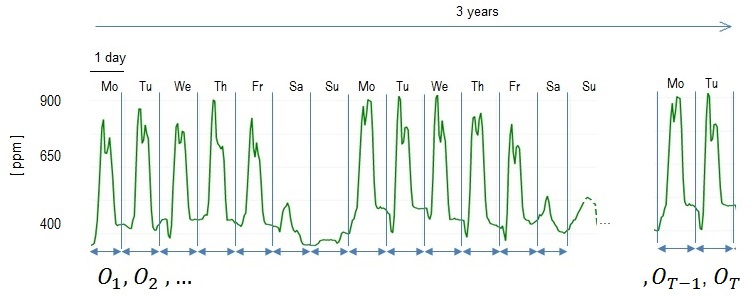
\includegraphics[scale=0.7]{Figures/split_time_series.jpg}
  \caption{ The $CO_2$ time series for the North-East ventilation system is split in a daily fashion. Each daily profile is an observed sample $O_i$.}
  \label{fig:daily_split}
\end{figure}

The observed sequence $\mathbb{O}$ is defined as a matrix of $24 \times 1081$ size. Each sample $O_i$ is a vector of length $L=24$ where each hour of the day has a corresponding value. Once the observed sequence is defined, the training process for the \textit{GaHMM - profile} is performed according to section \ref{sec:training_process} (\textit{ 4.hmm\_learning\_per\_variable\_k-fold}). The best \textit{GaHMM - profile} model is found by maximizing the likelihood of $p(\mathbb{O}|\lambda)$. At the end of the process, once the best model is found, we assume that there is a hidden state $S_k$ that is responsible for generating a sample $O_i$. In this way, we can find the best match between the sequence of hidden states $\mathbb{S}$ and the observed sequence $\mathbb{O}$. Using the Viterbi's algorithm we can discover the hidden state sequence $\mathbb{S}$ and, in this way, perform the time-depending clustering. Figure \ref{fig:daily_cluster} shows a hypothetical example where the $CO_2$ time series is disaggregated by daily profiles $O_i$ and the observed sequence is matched with the hidden state sequence $\mathbb{S} = [2,5,0,4,2,4,1,6,3,3,0,2,4,1]$. Then using the identification $ID$ of the hidden states, we can cluster days with similar daily profiles. For practical purposes, we name each cluster with the number of the associated hidden state (i.e. $ID = S_k$).  


\begin{figure}[h!]
  \vspace{0.5em} %better style
  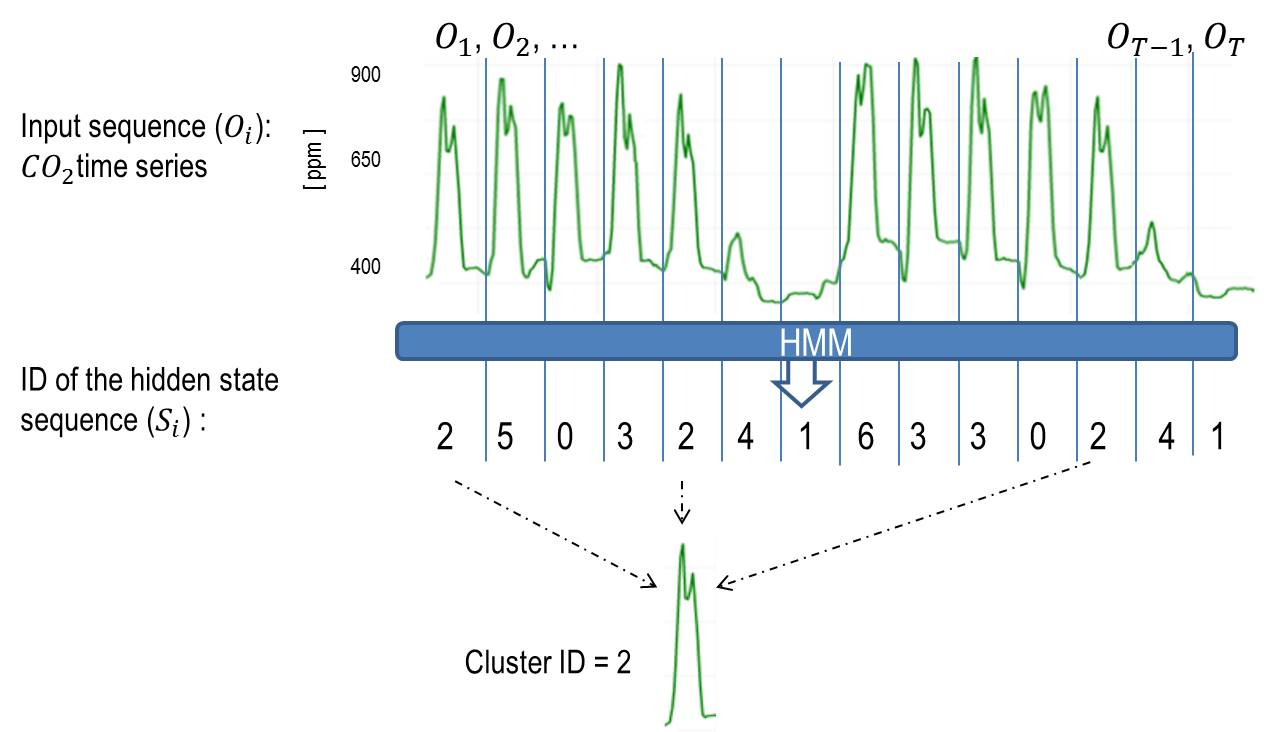
\includegraphics[scale=0.7]{Figures/sequence_explanation.jpg}
  \caption{Hypothetical example: The $CO_2$ time series is "emitted" by a $GaHMM$ model of 7 hidden states. $\mathbb{S} = [2,5,0,4,2,4,1,6,3,3,0,2,4,1]$. At the bottom-center the daily profile for cluster $ID=2$ corresponding to the hidden state $S_k=2$.}
  \label{fig:daily_cluster}
\end{figure}

The results of this model are discussed in section \ref{section:CO2_analysis} where the model is applied over the $CO_2$ time series in a case study. The quality of the cluster is reflected directly in the log probability of $p(\mathbb{O}|\lambda)$ and the average of $p(\mathbb{O}|\mathbb{S})$. However, to get a visual evaluation of the model, each cluster can be plotted out using box plots. A good cluster is one who has few (if any) outliers (i.e. fliers) outside of the whiskers. Examples of these daily profile clusters are in annex \ref{fig:candidates_profiles_NE}.


\subsection{GaHMM - seasonal model}
\label{sec:seasonal_model}

Several factors affect the way in which a building performs during the day. One of them is without a doubt, the outdoor conditions \cite{miller2015forensically, miller2015automated, djamila2017indoor}. The main purpose of this model is to cluster days according to the similarity of the outdoor conditions. In this way, we can use the information for understanding the dynamics of the building across seasons. For this purpose, the available \textbf{weather variables} (i.e. \textit{Outdoor temperature of the building, sunshine presence, precipitation and weather temperature}) are used for finding seasonal groups in the dataset. 


\paragraph{Implementation}  

A daily sample $O_i$ for this model is defined as a vector that contains selected features from the different weather variables. For practical purposes, this vector is herein called as $S_{vector}$. Features from the weather variables are calculated in a daily fashion \footnote{script \textit{2.statistics daily.py}}. Afterwards the entropy value for each feature is calculated by using the Kullback–Leibler divergence distance \footnote{Script: \textit{2.entropy\_calculation.py}} according to section \ref{sec:feature_selection}). This last value and the training process of the \textit{GaHMM} allows us to perform the feature selection in an indirect fashion. The final seasonal model uses only six features of a list of nineteen features (annex \ref{tab:feature_list}). These six selected features \footnote{The selection feature is done in an indirectly fashion by the training process, see in section \ref{sec:seasonal_evaluation}. The best model is reached by using six features among all, observe table \ref{tab:feature_gain} where the best features are in orange color} present in general, the maximum values of entropy among the list of features. Table \ref{tab:feature_gain} shows the gain of information of each individual feature, the bigger the value is, the more information we gain. This information can be retrieved from the \textit{'feature selection'} collection. In this way, each feature can be ranked according its gain of information. Thus, $F_1$ gains more information with and $F_{19}$ gains the less. In this way, from a collection of $m$ variables, a daily sample $O_i$ contains $f$ features of each variables $V$, that is:


% Please add the following required packages to your document preamble:
% \usepackage[table,xcdraw]{xcolor}
% If you use beamer only pass "xcolor=table" option, i.e. \documentclass[xcolor=table]{beamer}
\begin{table}[]
\centering
\caption{Entropy value $J$ for the \textit{weather variables}. It shows the gain of information for each variable according to section \ref{sec:feature_selection}. Definition of each feature in annex \ref{tab:feature_list}.}
\scriptsize
\label{tab:feature_gain}
\begin{tabular}{|l|l|l|l|l|l|l|l|l|lll}
\cline{1-3} \cline{5-6} \cline{8-9} \cline{11-12}
\multicolumn{1}{|c|}{\textit{\textbf{}}} & \multicolumn{2}{c|}{\cellcolor[HTML]{9AFF99}\textit{\textbf{Sunshine presence}}}                                                       & \multicolumn{1}{c|}{\textit{\textbf{}}} & \multicolumn{2}{c|}{\cellcolor[HTML]{9AFF99}\textit{\textbf{Outdoor temperature}}}                                                     & \multicolumn{1}{c|}{\textit{\textbf{}}} & \multicolumn{2}{c|}{\cellcolor[HTML]{9AFF99}\textit{\textbf{Weather Temperature}}}                                                     & \multicolumn{1}{c|}{\textit{\textbf{}}} & \multicolumn{2}{c|}{\cellcolor[HTML]{9AFF99}\textit{\textbf{Precipitation}}}                                                           \\ \cline{1-3} \cline{5-6} \cline{8-9} \cline{11-12} 
\multicolumn{1}{|c|}{\textit{\textbf{}}} & \multicolumn{1}{c|}{\cellcolor[HTML]{9AFF99}\textit{\textbf{f}}} & \multicolumn{1}{c|}{\cellcolor[HTML]{9AFF99}\textit{\textbf{J(f)}}} & \multicolumn{1}{c|}{\textit{\textbf{}}} & \multicolumn{1}{c|}{\cellcolor[HTML]{9AFF99}\textit{\textbf{f}}} & \multicolumn{1}{c|}{\cellcolor[HTML]{9AFF99}\textit{\textbf{J(f)}}} & \multicolumn{1}{c|}{\textit{\textbf{}}} & \multicolumn{1}{c|}{\cellcolor[HTML]{9AFF99}\textit{\textbf{f}}} & \multicolumn{1}{c|}{\cellcolor[HTML]{9AFF99}\textit{\textbf{J(f)}}} & \multicolumn{1}{c|}{\textit{\textbf{}}} & \multicolumn{1}{c|}{\cellcolor[HTML]{9AFF99}\textit{\textbf{f}}} & \multicolumn{1}{c|}{\cellcolor[HTML]{9AFF99}\textit{\textbf{J(f)}}} \\ \cline{1-3} \cline{5-6} \cline{8-9} \cline{11-12} 
$F_1$                                        & \cellcolor[HTML]{FFCE93}r\_factor\_st                            & \cellcolor[HTML]{FFCE93}inf                                         &                                         & \cellcolor[HTML]{FFCE93}r\_factor\_ed                            & \cellcolor[HTML]{FFCE93}1.00                                        &                                         & \cellcolor[HTML]{FFCE93}r\_factor\_ed                            & \cellcolor[HTML]{FFCE93}1.00                                        & \multicolumn{1}{l|}{}                   & \multicolumn{1}{l|}{\cellcolor[HTML]{FFCE93}max\_ed}             & \multicolumn{1}{l|}{\cellcolor[HTML]{FFCE93} inf}                       \\ \cline{1-3} \cline{5-6} \cline{8-9} \cline{11-12} 
$F_2$                                        & \cellcolor[HTML]{FFCE93}r\_factor\_ed                            & \cellcolor[HTML]{FFCE93}0.23                                        &                                         & \cellcolor[HTML]{FFCE93}r\_factor                                & \cellcolor[HTML]{FFCE93}0.51                                        &                                         & \cellcolor[HTML]{FFCE93}r\_factor                                & \cellcolor[HTML]{FFCE93}0.98                                        & \multicolumn{1}{l|}{}                   & \multicolumn{1}{l|}{\cellcolor[HTML]{FFCE93}(max-min)*std}       & \multicolumn{1}{l|}{\cellcolor[HTML]{FFCE93} inf}                       \\ \cline{1-3} \cline{5-6} \cline{8-9} \cline{11-12} 
$F_3$                                        & \cellcolor[HTML]{FFCE93}min\_me                                  & \cellcolor[HTML]{FFCE93}0.01                                        &                                         & \cellcolor[HTML]{FFCE93}(max-min)*std                            & \cellcolor[HTML]{FFCE93}0.24                                        &                                         & \cellcolor[HTML]{FFCE93}(max-min)*std                            & \cellcolor[HTML]{FFCE93}0.59                                        & \multicolumn{1}{l|}{}                   & \multicolumn{1}{l|}{\cellcolor[HTML]{FFCE93}25\%}                & \multicolumn{1}{l|}{\cellcolor[HTML]{FFCE93}4.53}                   \\ \cline{1-3} \cline{5-6} \cline{8-9} \cline{11-12} 
$F_4$                                        & \cellcolor[HTML]{FFCE93}max\_st                                  & \cellcolor[HTML]{FFCE93}0.01                                        &                                         & \cellcolor[HTML]{FFCE93}r\_factor\_st                            & \cellcolor[HTML]{FFCE93}0.21                                        &                                         & \cellcolor[HTML]{FFCE93}std                                      & \cellcolor[HTML]{FFCE93}0.42                                        & \multicolumn{1}{l|}{}                   & \multicolumn{1}{l|}{\cellcolor[HTML]{FFCE93}min\_me}             & \multicolumn{1}{l|}{\cellcolor[HTML]{FFCE93}1.98}                   \\ \cline{1-3} \cline{5-6} \cline{8-9} \cline{11-12} 
$F_5$                                        & \cellcolor[HTML]{FFCE93}max\_ed                                  & \cellcolor[HTML]{FFCE93}0.01                                        &                                         & \cellcolor[HTML]{FFCE93}dev\_u                                   & \cellcolor[HTML]{FFCE93}0.17                                        &                                         & \cellcolor[HTML]{FFCE93}dev\_u                                   & \cellcolor[HTML]{FFCE93}0.31                                        & \multicolumn{1}{l|}{}                   & \multicolumn{1}{l|}{\cellcolor[HTML]{FFCE93}min}                 & \multicolumn{1}{l|}{\cellcolor[HTML]{FFCE93}1.82}                   \\ \cline{1-3} \cline{5-6} \cline{8-9} \cline{11-12} 
$F_6$                                        & \cellcolor[HTML]{FFCE93}mean                                     & \cellcolor[HTML]{FFCE93}0.01                                        &                                         & \cellcolor[HTML]{FFCE93}std                                      & \cellcolor[HTML]{FFCE93}0.16                                        &                                         & \cellcolor[HTML]{FFCE93}r\_factor\_st                            & \cellcolor[HTML]{FFCE93}0.31                                        & \multicolumn{1}{l|}{}                   & \multicolumn{1}{l|}{\cellcolor[HTML]{FFCE93}min\_ed}             & \multicolumn{1}{l|}{\cellcolor[HTML]{FFCE93}0.64}                   \\ \cline{1-3} \cline{5-6} \cline{8-9} \cline{11-12} 
$F_7$                                        & 50\%                                                             & 0.01                                                                &                                         & min\_ed                                                          & 0.10                                                                &                                         & max\_ed                                                          & 0.16                                                                & \multicolumn{1}{l|}{}                   & \multicolumn{1}{l|}{max\_me}                                     & \multicolumn{1}{l|}{0.13}                                           \\ \cline{1-3} \cline{5-6} \cline{8-9} \cline{11-12} 
$F_8$                                        & dev\_u                                                           & 0.01                                                                &                                         & max\_ed                                                          & 0.08                                                                &                                         & min                                                              & 0.15                                                                & \multicolumn{1}{l|}{}                   & \multicolumn{1}{l|}{dev\_u}                                      & \multicolumn{1}{l|}{0.12}                                           \\ \cline{1-3} \cline{5-6} \cline{8-9} \cline{11-12} 
$F_9$                                        & r\_factor                                                        & 0.01                                                                &                                         & 75\%                                                             & 0.07                                                                &                                         & min\_st                                                          & 0.15                                                                & \multicolumn{1}{l|}{}                   & \multicolumn{1}{l|}{std}                                         & \multicolumn{1}{l|}{0.11}                                           \\ \cline{1-3} \cline{5-6} \cline{8-9} \cline{11-12} 
$F_{10}$                                       & 75\%                                                             & 0.01                                                                &                                         & max                                                              & 0.06                                                                &                                         & max\_st                                                          & 0.13                                                                & \multicolumn{1}{l|}{}                   & \multicolumn{1}{l|}{min\_st}                                     & \multicolumn{1}{l|}{0.09}                                           \\ \cline{1-3} \cline{5-6} \cline{8-9} \cline{11-12} 
$F_{11}$                                       & r\_factor\_u                                                     & 0.00                                                                &                                         & 50\%                                                             & 0.06                                                                &                                         & 75\%                                                             & 0.12                                                                & \multicolumn{1}{l|}{}                   & \multicolumn{1}{l|}{max}                                         & \multicolumn{1}{l|}{0.09}                                           \\ \cline{1-3} \cline{5-6} \cline{8-9} \cline{11-12} 
$F_{12}$                                       & max\_me                                                          & 0.00                                                                &                                         & max\_st                                                          & 0.06                                                                &                                         & min\_me                                                          & 0.11                                                                & \multicolumn{1}{l|}{}                   & \multicolumn{1}{l|}{50\%}                                        & \multicolumn{1}{l|}{0.07}                                           \\ \cline{1-3} \cline{5-6} \cline{8-9} \cline{11-12} 
$F_{13}$                                       & max                                                              & 0.00                                                                &                                         & max\_me                                                          & 0.06                                                                &                                         & 25\%                                                             & 0.09                                                                & \multicolumn{1}{l|}{}                   & \multicolumn{1}{l|}{75\%}                                        & \multicolumn{1}{l|}{0.04}                                           \\ \cline{1-3} \cline{5-6} \cline{8-9} \cline{11-12} 
$F_{14}$                                       & (max-min)*std                                                    & 0.00                                                                &                                         & mean                                                             & 0.05                                                                &                                         & max\_me                                                          & 0.09                                                                & \multicolumn{1}{l|}{}                   & \multicolumn{1}{l|}{mean}                                        & \multicolumn{1}{l|}{0.02}                                           \\ \cline{1-3} \cline{5-6} \cline{8-9} \cline{11-12} 
$F_{15}$                                       & std                                                              & 0.00                                                                &                                         & min\_st                                                          & 0.05                                                                &                                         & min\_ed                                                          & 0.09                                                                & \multicolumn{1}{l|}{}                   & \multicolumn{1}{l|}{max\_st}                                     & \multicolumn{1}{l|}{0.02}                                           \\ \cline{1-3} \cline{5-6} \cline{8-9} \cline{11-12} 
$F_{16}$                                       & min                                                              & 0.00                                                                &                                         & min\_me                                                          & 0.04                                                                &                                         & max                                                              & 0.09                                                                & \multicolumn{1}{l|}{}                   & \multicolumn{1}{l|}{r\_factor\_ed}                               & \multicolumn{1}{l|}{0.02}                                           \\ \cline{1-3} \cline{5-6} \cline{8-9} \cline{11-12} 
$F_{17}$                                       & min\_ed                                                          & 0.00                                                                &                                         & 25\%                                                             & 0.04                                                                &                                         & 50\%                                                             & 0.07                                                                & \multicolumn{1}{l|}{}                   & \multicolumn{1}{l|}{r\_factor\_st}                               & \multicolumn{1}{l|}{0.01}                                           \\ \cline{1-3} \cline{5-6} \cline{8-9} \cline{11-12} 
$F_{18}$                                       & 25\%                                                             & 0.00                                                                &                                         & min                                                              & 0.03                                                                &                                         & mean                                                             & 0.07                                                                & \multicolumn{1}{l|}{}                   & \multicolumn{1}{l|}{r\_factor\_u}                                & \multicolumn{1}{l|}{0.01}                                           \\ \cline{1-3} \cline{5-6} \cline{8-9} \cline{11-12} 
$F_{19}$                                       & min\_st                                                          & 0.00                                                                &                                         & r\_factor\_u                                                     & 0.02                                                                &                                         & r\_factor\_u                                                     & 0.05                                                                &                                         & r\_factor                                                        & 0.01                                                                \\ \cline{1-3} \cline{5-6} \cline{8-9} \cline{11-12}
\end{tabular}
\end{table}




\begin{equation}
\begin{array}{lc}
 & O_i = S_{vector}= [F_1^1, F_2^1,... F_f^1, F_1^2, F_2^2,...F_f^2, ...., F_1^m,F_2^m, ...F_f^m] \\
where: &  \\ 
& F_1^i, F_2^i,... F_f^i \in V_i \quad i \in [1,m] \\

\end{array}
\end{equation}

In the end, the observed sequence $\mathbb{O}$ is a matrix of $fm \times 1081$ size. Each sub-sequence of features $O_i$ for each day during the entire timeline (1081 days). Since the observed sequence is defined, the training process is performed according to section \ref{sec:training_process}. The clustering quality of this model is evaluated on section \ref{sec:seasonal_evaluation}, and the results of the best trained model are exposed and discussed in section\ref{sec:seasonal_results}. 

\subsection{GaHMM - interactional model}
\label{sec:interactional_model}

This model attempts to cluster days where the interaction between variables of the building dataset behave similarly. For this purpose, we use the Pearson correlation coefficient ($r$) to measure the linear correlation between two variables $X_1$ and $X_2$ \footnote{$X_1$ and $X_2$ are time series of the building dataset. It could be the entire time series or just a selected period.}. r varies between — 1 and +1, which represent perfect negative and perfect positive linear relationships, respectively. When r = 0, there is no linear correlation between the variables \cite{cohen2013applied}. To perform a multivariate analysis of variables in the building data set, a Pearson correlation matrix is created using a set of variables $V = [X_1, X_2, .., X_n]$, as follows: 

\begin{equation}
R = 
\begin{pmatrix} r(X_1,X_1) &  r(X_1,X_2) & ... & r(X_1,X_n) \\ 
				r(X_2,X_1) &  r(X_2,X_2) & ... & r(X_2,X_n) \\
				...        &  ...        & ... & ... \\ 
				r(X_n,X_1) &  r(X_n,X_2) & ... & r(X_n,X_n)\end{pmatrix} 
\end{equation}

Where $X_i = [x_1, x_2, ..., x_T]$ is an individual time series of length $T$ of the set of variables $V$ and the individual Pearson correlation coefficient (r) between two time series $X$ and $Y$ is calculated by:

\begin{equation}
r(X,Y) =  \dfrac{\sum_{k=1}^T (x_k - \overline{x})(y_k - \overline{y})}{ \sqrt{\sum_{k=1}^T (x_i - \overline{x})^2} \sqrt{\sum_{k=1}^T (y_i - \overline{y})^2} }
\end{equation}

In our approach, the $R$ matrix is calculated in a daily fashion, so that each time series has a length $T=24$. For the whole timeline, 1081 matrices of size $n \times n$ are saved in the 'correlation\_matrix\_daily' collection by the script \textit{2.correlation\_matrix\_v1\_daily}. We define two sets of variables $V$, one for each part of the building. That is $V_1$ for the North-Eastern part and $V_2$ for the South-Western part of the building. In addition, the weather variables are included in both sets. This matrix allows the visualization of the average Pearson correlation coefficient $\overline{r}$ between variables by using a Hierarchical Edge Bundles \footnote{Web server (\textit{Flask\_project.py}): \url{http://127.0.0.1:5000/correlation}} visualization \ref{sec:edge}, see figure \ref{aver}.


\begin{equation}
\overline{r} (X,Y) = \frac{1}{L} \sum_{i=0}^L r(X_i,Y_i)
\label{aver}
\end{equation}


\begin{figure}[h!]
  \vspace{0.5em} %better style
  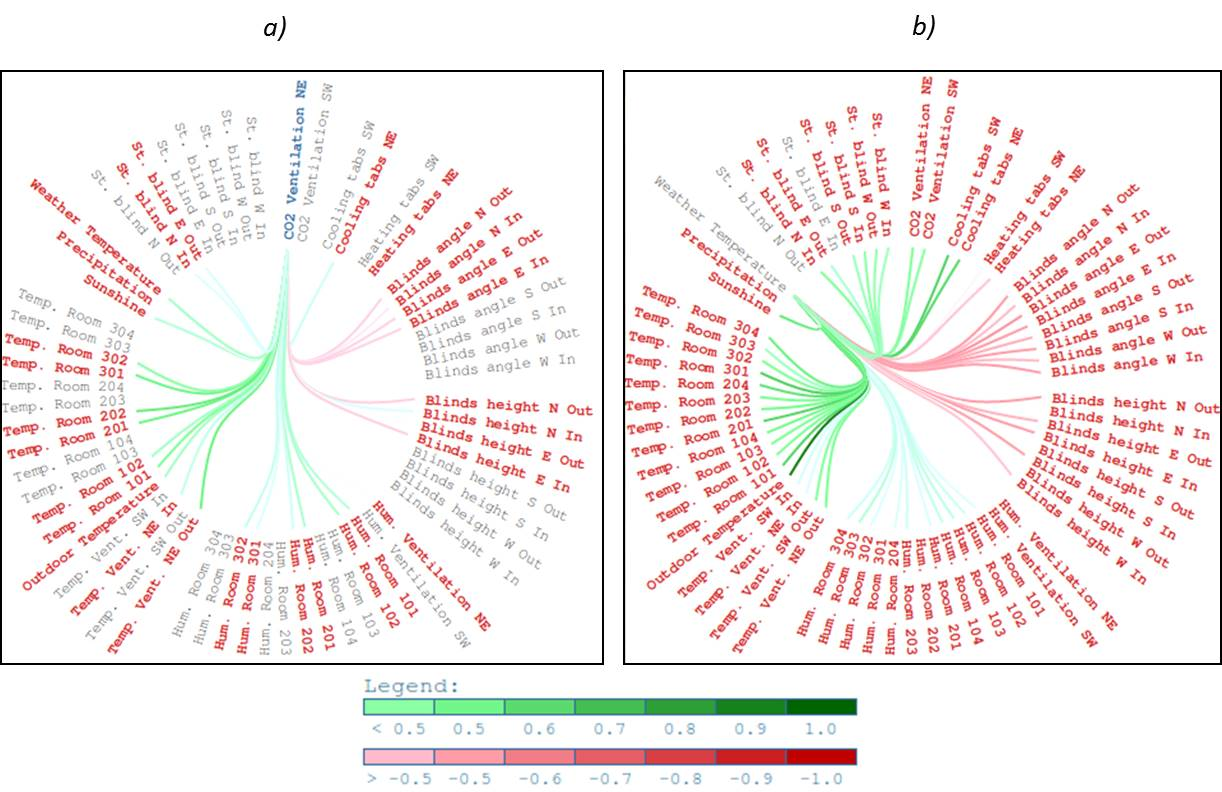
\includegraphics[scale=0.65]{Figures/flor_correlation.jpg}
  \caption{Average value of the Pearson correlation coefficient for variables of the building dataset. \textit{a)} Variables correlated with the measures of $CO_2$ levels of the North-East ventilation system. \textit{b)} Variables correlated with the weather temperature measures.}
  \label{fig:edge}
\end{figure}


\begin{figure}[h!]
  \vspace{0.5em} %better style
  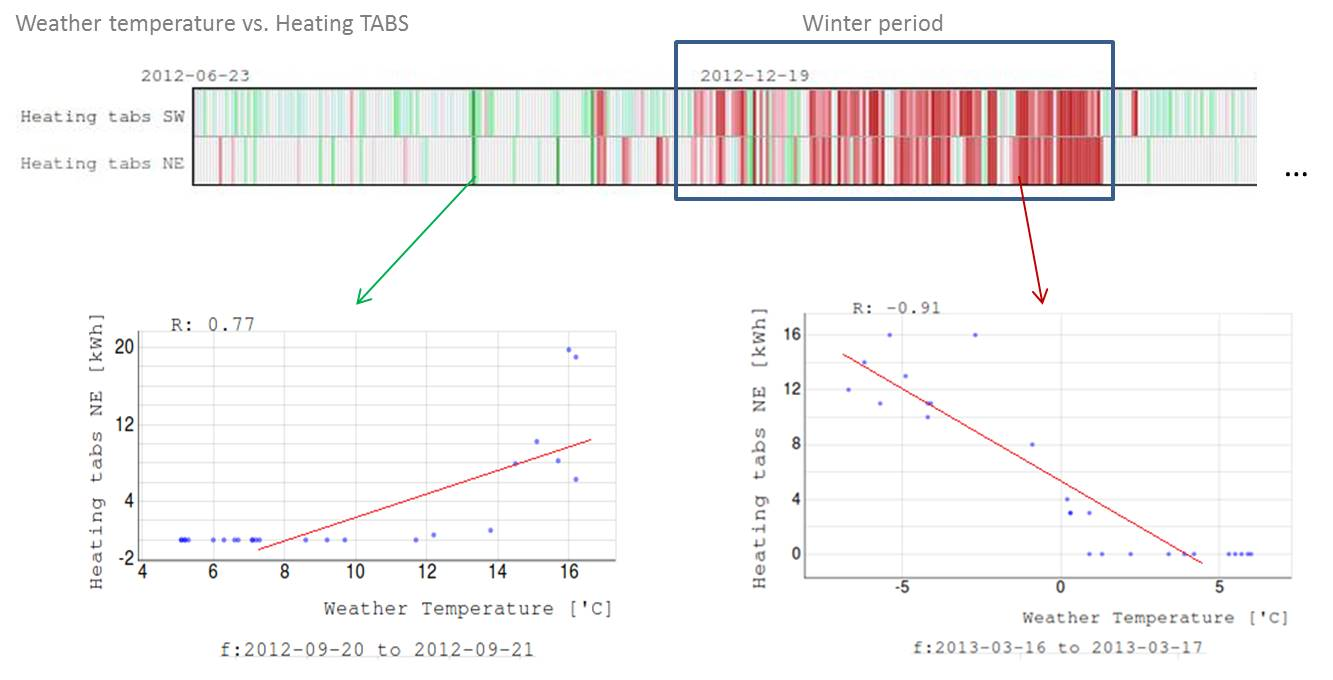
\includegraphics[scale=0.65]{Figures/heatmap.jpg}
  \caption{Average value of the Pearson correlation coefficient for variables of the building dataset. \textit{a)} Variables correlated with the measures of $CO_2$ levels of the North-East ventilation system. \textit{b)} Variables correlated with the weather temperature measures.}
  \label{fig:heatmap}
\end{figure}

The average value of the Pearson correlation coefficient is calculated by equation \ref{aver} where $X_i$ and $Y_i$ are a daily time series, and $L$ is total number of daily time series. Figure \ref{fig:edge} shows in red and green colors, the average values of $r$ during the entire timeline. The green color implies a positive correlation while the red implies a negative correlation between variables. The reason for a pair of variables having a $\overline{r}$ value close to zero, is because there is either no correlation between them or because the correlation changes frequently depending on the season and/or the day of the week (i.e. going from positive to negative and vice versa). This is the case for instance of the correlation between weather temperature (°C) and heating TABS energy consumption (kWh). Figure \ref{fig:heatmap} refers to the aforementioned case. It  is clear to see how the correlation between these two variables changes during the winter period. Furthermore, the fact that the
heating TABS of the South-West part of the building has more slightly positive correlation than the North-East part (when not in the winter period), is remarkable. This is the reason why the $\overline{r}$ value for the south-west TABS is close to zero (see \ref{fig:edge} {\color{red} .\textit{b)}}).  

The \textit{GaHMM - interactional} model uses the information from the matrix $R$. Each observed samples $O_i$ is defined by a vector called $R_{vector}$. This vector contains the $r$ value for variables of interest. 

\begin{equation}
O_i = R_{vector} (X_i) = [r(X_i,X_1), r(X_i, X_2), ..., r(X_i, X_n)]
\label{r_vector}
\end{equation}

For our proposed model, $X_i$ refers to the $CO_2$ levels of the North-East or South-West ventilation systems. The variables $X_1, ..., X_n$ correspond to different zones of the building (i.e. North-East or South-West). In this way, two $R_{vector}$ are defined for each zone in a daily fashion. Since the observed sample $O_i$ is defined, the training process can be performed according to section \ref{sec:training_process}. The evaluation and results of this model are exposed and discussed on sections \ref{sec:interactional_evaluation}, \ref{sec:interactional_results}.  


\section{Hierarchical Agglomerative Clustering}
\label{sec:hierar_agg}


In this section, we adapt the concepts that were explained in section \ref{hierarchical}, therefore in our context, an object is called a cluster profile. Since clustering is the grouping of similar objects, one can use different measures to determine whether two objects are similar or dissimilar. There are two main type of measures used to estimate similarity: distance measures and similarity measures \cite{maimon2007soft}. Normally, distance measures are used for determining the similarity between two objects in the HAC approach. Here a brief list of some of them: \textit{Euclidean distance, squared Euclidean distance, city-block (Manhattan) distance, Chebychev distance, power distance, Mahalanobis distance}. We do not go in details about each dissimilarity/similarity distance, the reader can find details in \cite{maimon2007soft,saraccli2013comparison,mullner2011modern}. However we consider important to add the definition of the euclidean distance (equation \ref{equa1}), for exemplification purposes: 

\begin{equation}
\label{equa1}
 \displaystyle d(p,q)={\sqrt {(p_{1}-q_{1})^{2}+(p_{2}-q_{2})^{2}+\cdots +(p_{i}-q_{i})^{2}+\cdots +(p_{n}-q_{n})^{2}}} 
\end{equation} 

$d(p,q)$ is the euclidean distance of two daily profiles $p$ and $q$, where $p_i$ corresponds to a measure value that belongs to the daily profile $p$. The Hierarchical agglomerative clustering creates a distance matrix $D$ using a distance measure. For example, table \ref{fig:matrix_1} is the distance matrix of 5 hypothetical daily profiles, where profiles 3 and 5 are the closest ones. This implies the first hierarchical cluster (i.e. $id= 35$). 

\begin{figure}[h!]
  \vspace{0.5em} %better style
  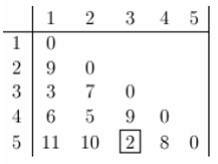
\includegraphics[scale=0.65]{Figures/distance_matrix_1.jpg}
  \caption{Distance matrix $D$ of 5 hypothetical daily profiles, using the euclidean distance. First interaction.}
  \label{fig:matrix_1}
\end{figure}

Now the distance between any cluster profile against the hierarchical cluster $id=35$ should be defined. This new similarity distance between hierarchical nodes is what is called as linkage method. There are different methods for linkage: \textit{Single link, Complete link, Group average, Ward’s method, etc.}. The reader is invited to refer more information about linkage methods in \cite{maimon2007soft,saraccli2013comparison,mullner2011modern}. We include in equation \ref{equa2} the group average linkage method, for illustration purposes:

\begin{equation}
\label{equa2}
    d ( A , B ) = \dfrac{1}{|A| \cdot |B|} \sum_{p \in A} \sum_{q \in B} d(p,q)
\end{equation} 

$d(A ,B)$ implies the distance that exists between hierarchical clusters $A$ and $B$ using the average linkage method. A hierarchical cluster collapse similar objects where dissimilarity distance is the smallest. Table \ref{fig:matrix_2} shows the case when the profile cluster $3$ and $5$ are collapsed in one hierarchical cluster $35$. The distances within the distance matrix $D$ are calculated by using equation \ref{equa2}.  

\begin{figure}[h!]
  \vspace{0.5em} %better style
  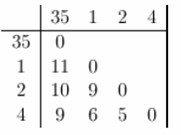
\includegraphics[scale=0.65]{Figures/distance_matrix_2.jpg}
  \caption{Distance matrix $D$ of 5 hypothetical daily profiles, using the euclidean distance. Second interaction.}
  \label{fig:matrix_2}
\end{figure}

In a new interaction, the new hierarchical cluster is $ID=24$ since the distance between profile $2$ and $4$ is the shortest one. New interactions are performed until the total reduction of the distance matrix $D$. The result of the hierarchical clustering can be displayed in a tree-like structure, called a dendrogram (see figure \ref{fig:dendogram_total}), with one cluster at the top containing all the objects, and each branch groups similar objects. 

\begin{figure}[h!]
  \vspace{0.5em} %better style
  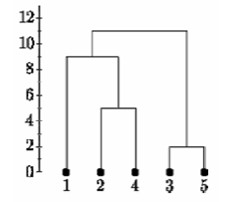
\includegraphics[scale=0.65]{Figures/dendogram_result.jpg}
  \caption{Resulting dendrogram from the distance matrix $D$.}
  \label{fig:dendogram_total}
\end{figure}


This is the process to perform a hierarchical agglomerative clustering with cluster profiles. We indicate in a practical way, how this clustering is performed in section \ref{sec:discord_finding}. In addition, a measure (i.e. \textit{Cophenetic correlation coefficient}) for knowing how faithfully a dendrogram preserves the pairwise distances between the original unmodeled data points is used. This measure allows to know which distance metric and linkage method is the most appropriated for the data \cite{saraccli2013comparison}. 

\section{Evaluation}
\label{sec:eval_all}

\subsection{Evaluation of the \textit{GaHMM - profile} model}
\label{sec:profile_evaluation}

Our approach trains a \textit{GaHMM-profile model} for each variable of the data set. This training process is done according to \ref{sec:training_process} \footnote{Script: \textit{4.hmm\_learning\_per\_variable\_k-fold.py}}. The best model is elected by using the log probability of $ p(\mathbb{O}|\lambda)$ and the results are presented as the average of $p(\mathbb{O}|\mathbb{S})$. A box plot is proposed to see the quality of the cluster profiles. Figure \ref{fig:box_plot} shows \textbf{a)} a profile cluster of a poor trained \textit{GaHMM - profile} (i.e. $\overline{p}(\mathbb{O}|\mathbb{S}) = 0.885 $, $n_{component}=9$ ) of the $CO_2$ measures of the North-East ventilation system,  one can see the amount of outliers (i.e. fliers) outside of the whiskers, in contrast with \textbf{b)} a profile cluster of the best trained \textit{GaHMM - profile} (i.e. $\overline{p}(\mathbb{O}|\mathbb{S}) = 0.993 $, $n_{component}=33$) where there are only 4 outliers.   

\begin{figure}[h!]
  \vspace{0.5em} %better style
  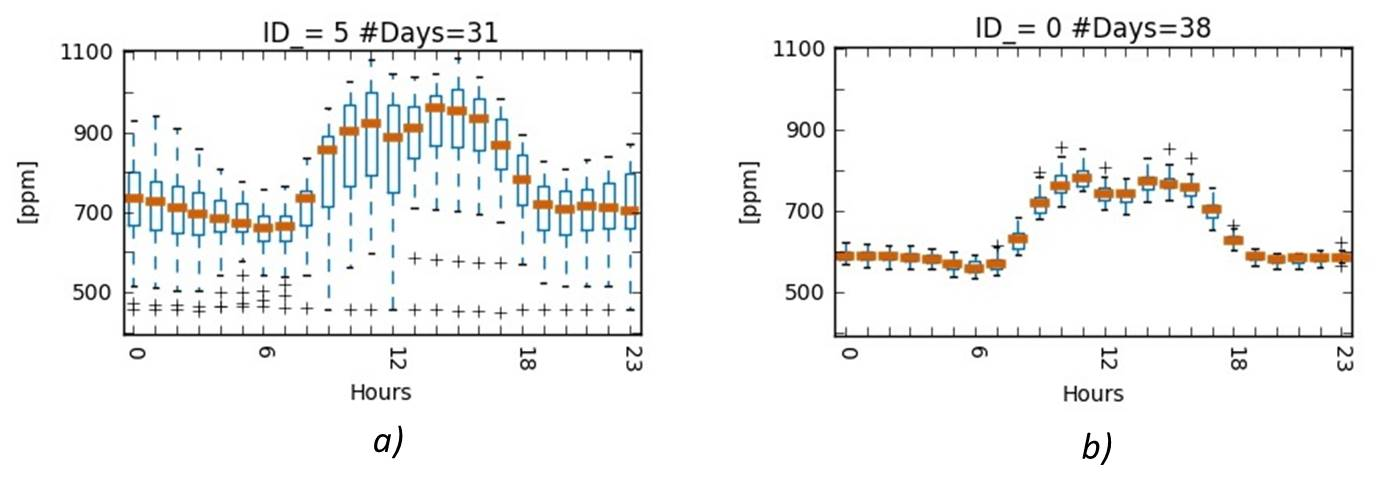
\includegraphics[scale=0.65]{Figures/box_plot.jpg}
  \caption{ $CO_2$ cluster profile of 
  a)  \textit{GaHMM - profile} with $\overline{p}(\mathbb{O}|\mathbb{S}) = 0.885, n_{component}=9 $ b) \textit{GaHMM - profile} with $\overline{p}(\mathbb{O}|\mathbb{S}) = 0.993, n_{component}=33$.}
  \label{fig:box_plot}
\end{figure} 


It follows then that, cluster profiles which belong to the best \textit{GaHMM - profile} models have tiny standard deviations for each hour of the day and there are no outliers (the number of outliers is less than 10\% of the whole samples). In this way, one obtains a good representation of the existing daily profiles. This is how each \textit{GaHMM - profile} model is evaluated. Table \ref{tab:profile_model_eval} shows the evaluation of the models that are used in a
case study (section \ref{section:CO2_analysis}). Additionally, one can see the quality of clusters in annex \ref{cluster_profiles} and the digital folder annex: iPythonBooks/Diversity of profiles.


% Table generated by Excel2LaTeX from sheet 'Hoja2'
\begin{table}[htbp]
  \centering
  \scriptsize
  \caption{Example of evaluation of \textit{GaHMM - profile} models for different variables}
    \begin{tabular}{|l|r|r|r|r|r|}
    \hline
    Variable & \multicolumn{1}{l|}{TABS Cooling NE} & \multicolumn{1}{l|}{TABS Heating NE} & \multicolumn{1}{l|}{Exhaust Air Temperature} & \multicolumn{1}{l|}{Intake air temperature} & \multicolumn{1}{l|}{$CO_2$ NE} \bigstrut\\
    \hline
    $\overline{p}(\mathbb{O}|\mathbb{S})$ & 0.9997 & 0.9982 & 0.9963 & 0.9976 & 0.9932 \bigstrut\\
    \hline
    $n_{components}$ & 33   & 32   & 31   & 33   & 33 \bigstrut\\
    \hline
    \end{tabular}%
  \label{tab:profile_model_eval}%
\end{table}%


\subsection{Evaluation of the \textit{GaHMM - seasonal} model}
\label{sec:seasonal_evaluation}


A \textit{GaHMM - seasonal} model is trained according to section \ref{sec:training_process} \footnote{script \textit{4.hmm\_learning\_k-fold.py}}  and \ref{sec:seasonal_model}. To evaluate a \textit{GaHMM - seasonal} model, we propose the use of log probability of $ p(\mathbb{O}|\lambda)$, average of $p(\mathbb{O}|\mathbb{S})$ and a visualization of the $S_{vector}$ in 3D space by using PCA. Table \ref{tab:result_training_seasonal} shows the evaluation of the best trained models for different number of features $ f $ and different number of hidden states $n$ according to sections \ref{sec:training_process} and \ref{sec:seasonal_model}. The selected variables for this table are the outdoor temperature of the building and the weather temperature. One can observe that the average of $p(\mathbb{O}|\mathbb{S})$ improves as we add new features but this diminishes after $f = 6$. The tendency is that the more features and variables we use to train the model, the more hidden states we need to describe the clusters. The observed sample $O_i$ becomes more scattered and therefore more clusters are needed, however even if we increase the number of hidden states, we do not get the same results that were achieved by the model with $f = 6$ and
$n = 2; 3; 4$.

Since the best results are achieved with $n=2,3,4$, we can choose to group the seasonal patterns in 2 or 3 or 4 clusters. We decide to group the patterns in four latent groups. They were named as \textit{summer, winter, coldest transition and hottest transition} due to the distribution of each cluster, this can be observed in figure \ref{fig:monthly}. Notice that names spring and autumn were not included in the list because when one sees the monthly distribution of the clusters, one can observe that the seasonal period of spring and autumn share some patterns in common. This last fact is explained further on section \ref{sec:seasonal_results}. 



%-------------------------------------------
%------------------------------------------------------------

% Table generated by Excel2LaTeX from sheet 'Feature Selection'
\begin{table}[htbp]
  \centering
  \scriptsize
  \caption{Average of $p(\mathbb{O}|\mathbb{S})$ for different \textit{GaHMM} models using $f$ features of outdoor temperature and weather temperature variables. }
      \begin{tabular}{|l|r|r|r|r|r|r|r|r|r|}
    \hline
         & \multicolumn{1}{l|}{f = 3} & \multicolumn{1}{l|}{f = 4} & \multicolumn{1}{l|}{f = 5} & \multicolumn{1}{l|}{f = 6} & \multicolumn{1}{l|}{f = 7} & \multicolumn{1}{l|}{f = 9} & \multicolumn{1}{l|}{f = 10} & \multicolumn{1}{l|}{…} & \multicolumn{1}{l|}{f = 18} \bigstrut\\
    \hline
    n = 2 & \cellcolor[rgb]{ .773,  .851,  .945} \textbf{0.99109447} & 0.99153911 & 0.99178444 & \cellcolor[rgb]{ 1,  .753,  0} \textbf{0.99859934} & 0.98443497 & 0.98467069 & 0.97706896 &      & 0.9924231 \bigstrut\\
    \hline
    n = 3 & 0.98247032 & \cellcolor[rgb]{ .773,  .851,  .945} \textbf{0.99248157} & \cellcolor[rgb]{ .773,  .851,  .945} \textbf{0.99339644} & \cellcolor[rgb]{ 1,  .753,  0} \textbf{0.99963577} & 0.9746971 & 0.97469422 & 0.969422 &      & 0.9974565 \bigstrut\\
    \hline
    n = 4 & 0.97436977 & 0.98552845 & 0.98819893 & \cellcolor[rgb]{ 1,  .753,  0} \textbf{0.99889142} & \cellcolor[rgb]{ .773,  .851,  .945} \textbf{0.98574802} & \cellcolor[rgb]{ .773,  .851,  .945} \textbf{0.98505652} & 0.96177504 &      & 0.9956667 \bigstrut\\
    \hline
    n = 5 & 0.97249754 & 0.98488397 & 0.98415621 & 0.99113528 & 0.98121257 & 0.9791666 & \cellcolor[rgb]{ .773,  .851,  .945} \textbf{0.9791666} &      & \cellcolor[rgb]{ .773,  .851,  .945} \textbf{0.9992562} \bigstrut\\
    \hline
    \end{tabular}%
  \label{tab:result_training_seasonal}%
\end{table}%

\begin{figure}[h!]
  \vspace{0.5em} %better style
  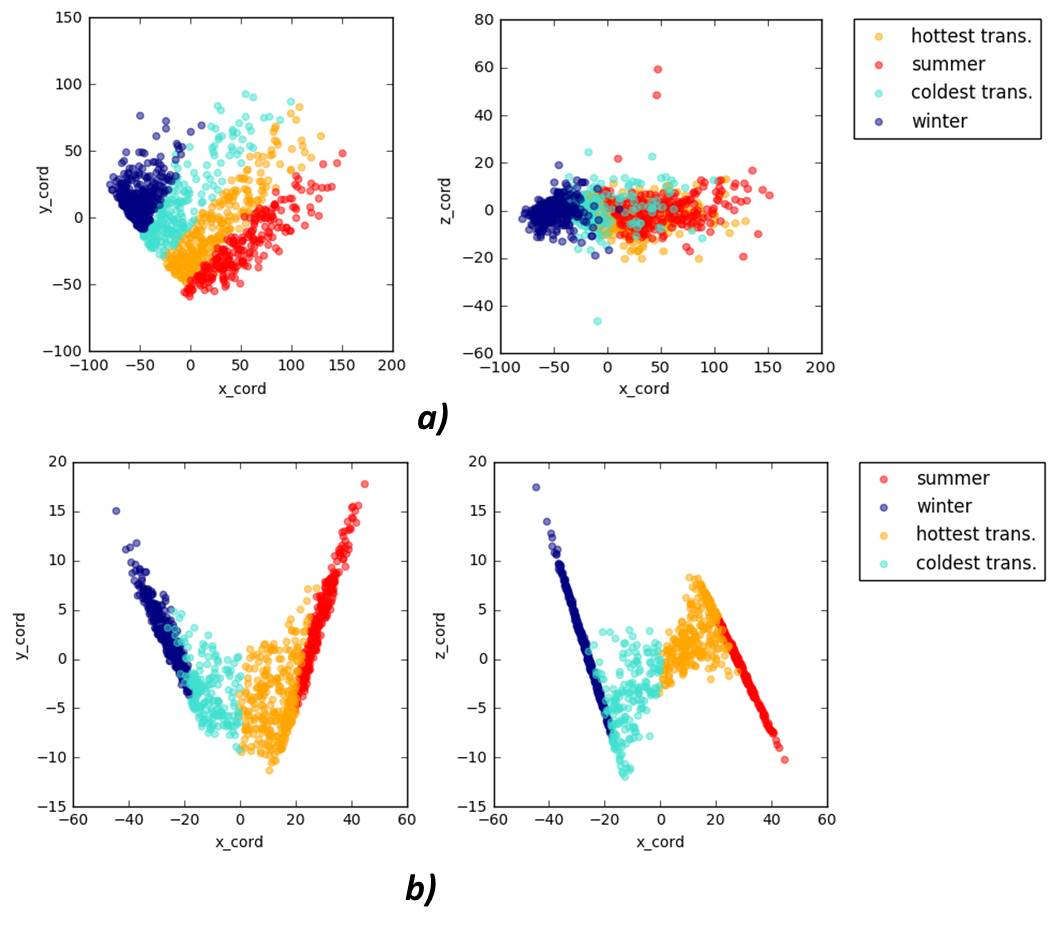
\includegraphics[scale=0.73]{Figures/PCA_visualization_C1-C4.jpg}
  \caption{Dimensional reduction using PCA for visualization: a) Visualization of $S_{vector}$ with 18 features b) Visualization of $S_{vector}$ with 6 features. Colors according to the trained \textit{GaHMM} seasonal models.}
  \label{fig:PCA_visualization}
\end{figure} 


One can observe the last fact by using the PCA procedure to transform the $S_{vector}$ to a new coordinate system, in this way, one can appreciate the quality of the clusters and the dispersion of the $S_{vector}$. Figure \ref{fig:PCA_visualization} shows the difference when \textbf{a)} we use a $S_{vector}$ of 18 features according
to annex \ref{tab:feature_list} and \textbf{b)} when we use a $S_{vector}$ of 6 features that have a good gain of information\footnote{The gain of information (i.e. entropy) was calculated and saved in 'feature\_selection' collection} according to \ref{sec:feature_selection}. Figure \ref{fig:PCA_visualization}{\color{red} .\textit{b)}} shows how the 6 features represent a good clustering quality. The results of the best GaHMM seasonal models are explained in section \ref{sec:seasonal_results}. 


\subsection{Evaluation of the \textit{GaHMM - interactional} model}
\label{sec:interactional_evaluation}

A \textit{GaHMM - interactional} model is trained according to section \ref{sec:training_process} \footnote{script \textit{4.hmm\_learning\_k-fold.py}} and \ref{sec:interactional_model}. To evaluate a \textit{GaHMM - interactional} model, we propose the use of log probability of $ p(\mathbb{O}|\lambda)$, average of $p(\mathbb{O}|\mathbb{S})$ and a visualization of the $R_{vector}$ in 3D space by using PCA. Table \ref{tab:result_interactional} shows the evaluation of the best trained models for different variables in $V_1$ and the different number of hidden states $n$ according to sections \ref{sec:training_process} and \ref{sec:interactional_model}. Each category is a group of different variables as is shown in annex (\ref{sec:metadata_t}, \textit{breakout\_group}).


% Table generated by Excel2LaTeX from sheet 'Category_selection'
\begin{table}[htbp]
  \centering
  \scriptsize
  \caption{$\overline{p}(\mathbb{O}|\mathbb{S})$ for each \textit{GaHMM interactional} model. The code of the selected categories are in annex \ref{sec:metadata_t}. These categories belongs to the North-East part of the building.}
    \begin{tabular}{|l|r|r|r|r|}
    \hline
    \textit{\textbf{Selected Categories}} & \multicolumn{1}{l|}{\textit{\textbf{n=2}}} & \multicolumn{1}{l|}{\textit{\textbf{n=3}}} & \multicolumn{1}{l|}{\textit{\textbf{n=4}}} & \multicolumn{1}{l|}{\textit{\textbf{n=5}}} \bigstrut\\
    \hline
    $[A\_6\_1, A\_6\_2, A\_6\_3]$ & \cellcolor[rgb]{ .573,  .804,  .863} 0.988713 & 0.977466 & 0.957416 & 0.960756 \bigstrut\\
    \hline
    \textcolor[rgb]{ 1,  0,  0}{$[A\_3, A\_{4\_1}, A\_{4\_2},  A\_{6\_1}, A\_{6\_2}]$} & 0.999950 & \cellcolor[rgb]{ 1,  .753,  0} 1.000000 & 0.999999 & 0.993509 \bigstrut\\
    \hline
    $[A\_{5\_1}, A\_{5\_2}, A\_{6\_1}, A\_{6\_2}, A\_{6\_3}]$ & \cellcolor[rgb]{ .573,  .804,  .863} 0.988981 & 0.976075 & 0.970061 & 0.977153 \bigstrut\\
    \hline
    $[A\_3, A\_{5\_1}, A\_{5\_2} , A\_{6\_1}, A\_{6\_2}, A\_{6\_3}]$ & 0.995121 & \cellcolor[rgb]{ .573,  .804,  .863} 0.997511 & 0.972120 & 0.979629 \bigstrut\\
    \hline
    $[A\_3, A\_{4\_1}, A\_{4\_2},  A\_{5\_1}, A\_{5\_2},  A\_{6\_3}]$ & 0.998842 & 0.997909 & \cellcolor[rgb]{ .573,  .804,  .863} 0.999975 & 0.985505 \bigstrut\\
    \hline
    $[A\_3, A\_{4\_1}, A\_{4\_2}, A\_{6\_1}, A\_{6\_2}, A\_{6\_3}]$ & \cellcolor[rgb]{ .573,  .804,  .863} 0.999599 & 0.998505 & 0.982654 & 0.984053 \bigstrut\\
    \hline
    $[A\_3, A\_{4\_1}, A\_{4\_2}, A\_{5\_1}, A\_{5\_2}, A\_{6\_1}, A\_{6\_2}]$ & \cellcolor[rgb]{ .573,  .804,  .863} 0.999978 & 0.999708 & 0.998038 & 0.985093 \bigstrut\\
    \hline
    $[A\_{4\_1}, A\_{4\_2}, A\_{5\_1},  A\_{5\_2}, A\_{6\_1}, A\_{6\_2}, A\_{6\_3}]$ & \cellcolor[rgb]{ .573,  .804,  .863} 0.992985 & 0.974719 & 0.963989 & 0.991043 \bigstrut\\
    \hline
    $[A\_3,  A\_ {4\_1}, A\_{4\_2}, A\_{5\_1}, A\_{5\_2}, A\_{6\_1}, A\_{6\_2}, A\_{6\_3}]$ & \cellcolor[rgb]{ .573,  .804,  .863} 0.993445 & 0.984509 & 0.974876 & 0.965273 \bigstrut\\
    \hline
    $[A\_1, A\_2, A\_3, A\_{4\_1}, A\_{4\_2}, A\_{5\_1}, A\_{5\_2}, A\_{6\_1}, A\_{6\_2}, A\_{6\_3}]$ & \cellcolor[rgb]{ .573,  .804,  .863} 0.999715 & 0.998432 & 0.997369 & 0.987582 \bigstrut\\
    \hline
    \end{tabular}%
  \label{tab:result_interactional}%
\end{table}%


\begin{table}[]
\centering
\scriptsize
\caption{Variables according to the category code:  \textit{[A\_3, A\_{4\_1}, A\_{4\_2},  A\_{6\_1}, A\_{6\_2}]}. The complete category code is in annex \ref{sec:metadata_t}.}
\label{code_cat}
\begin{tabular}{|l|l|}
\hline
Code    & Variables                                                                          \\ \hline
A\_3    & {[}Blinds angle N Out, Blinds angle N In, Blinds angle E Out, Blinds angle E In{]} \\ \hline
A\_4\_1 & {[}Blinds height N Out, Blinds height E In{]}                                      \\ \hline
A\_4\_2 & {[}Blinds height N In, Blinds height E Out{]}                                      \\ \hline
A\_6\_1 & {[}Temp. Vent. NE Out{]}                                                           \\ \hline
A\_6\_2 & {[}Temp. Vent. NE In{]}                                                            \\ \hline
\end{tabular}
\end{table}

The selected categories $[A\_3, A\_{4\_1}, A\_{4\_2},  A\_{6\_1}, A\_{6\_2}]$ (table \ref{code_cat}) is a group of variables that have a relevant linear correlation with the $CO_2$ levels of the North-East part of the building according to the evaluation in the table \ref{tab:result_interactional}. This fact is visible when one applies dimensionality reduction using PCA to project the $R_{vector}$ in a 3D space. Figure \ref{fig:PCA_categories} shows the PCA transformation where one appreciates the difference when \textbf{a)} $R_{vector}$ is defined by categories \textit{[A\_1, A\_2, A\_3, A\_4\_1, A\_4\_2, A\_5\_1, A\_5\_2, A\_6\_1, A\_6\_2]}, and \textbf{b)} $R_{vector}$ is defined by categories \textit{[A\_3, A\_{4\_1}, A\_{4\_2},  A\_{6\_1}, A\_{6\_2}]}. It is remarkable to see a good clustering quality in the case b) where all the three cluster are clearly defined. Clusters: [\textit{Regimen NC, Regimen WC, Regimen PC}] refers to Regimen of Negative Correlation, Weak Correlation and Positive Correlation. These clusters and the corresponding results are described in section \ref{sec:interactional_results}. As additional information, we observe the same behavior for the South-West part of the building (i.e. $V_2$ and categories $B\_*$). 

\begin{figure}[h!]
  \vspace{0.5em} %better style
  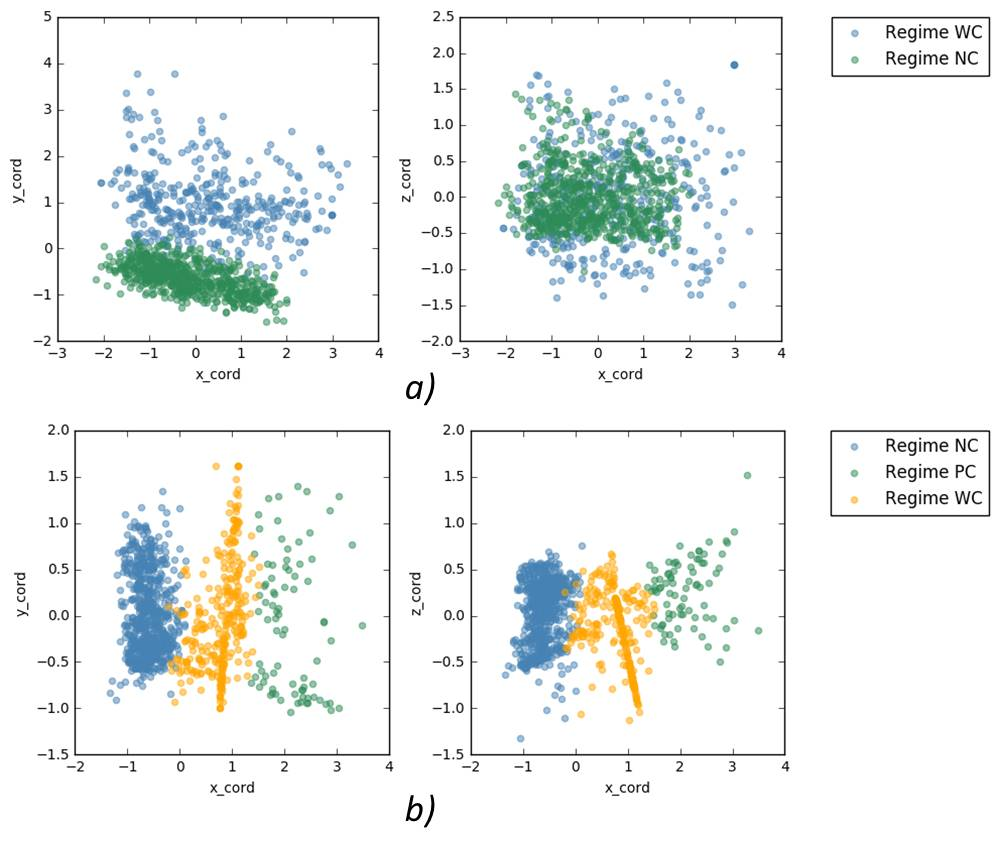
\includegraphics[scale=0.73]{Figures/Interactional_model_cluster.jpg}
  \caption{Dimensional reduction using PCA for visualization: a) Visualization of $R_{vector}$ using categories \textit{[A\_1, A\_2, A\_3, A\_4\_1, A\_4\_2, A\_5\_1, A\_5\_2, A\_6\_1, A\_6\_2]} b) Visualization of $R_{vector}$ using categories \textit{[A\_3, A\_{4\_1}, A\_{4\_2},  A\_{6\_1}, A\_{6\_2}]}. Colors according to the trained \textit{GaHMM} interactional models.}
  \label{fig:PCA_categories}
\end{figure}










 
% Chapter 2
\chapter{Results} % Main chapter title
\label{Chapter5} % For referencing the chapter elsewhere, use \ref{Chapter2} 
\minitoc
%----------------------------------------------------------------------------------------

%% Define some commands to keep the formatting separated from the content 
%\newcommand{\keyword}[1]{\textbf{#1}}
%\newcommand{\tabhead}[1]{\textbf{#1}}
%\newcommand{\code}[1]{\texttt{#1}}
%\newcommand{\file}[1]{\texttt{\bfseries#1}}
%\newcommand{\option}[1]{\texttt{\itshape#1}}

%----------------------------------------------------------------------------------------

This chapter presents the results of each evaluated model (i.e. \textit{GaHMM profile, seasonal and interactional}). The evaluation information, expossed in section \ref{sec:eval_all}, is used in conjuction with the results of each model in a study case where we compare the Noth-East and South-West ventilation systems. Furthermore, one practical application is proposed for the \textit{GaHMM} profile model. In the penultimate section, we include a comparison of our proposition (i.e. \textit{GaHMM profile model}) against \textit{DayFilter} approach that is considered as one of the state of art for AFDD \cite{kim2017review,miller2015automated}. At the end of this chapter, we include the feedback   from building control system specialists of Synergy BTC AG.

\section{Results}

\subsection{Results of the GaHMM seasonal model}
\label{sec:seasonal_results}

As it was explained in section \ref{sec:seasonal_evaluation}, we can evaluate a \textit{GaHMM seasonal} model by using the log probability of $p(\mathbb{O}|\lambda)$, average of $p(\mathbb{O}|\mathbb{S})$ and PCA visualization. 
Here we indicate how the clusters of \textit{summer, winter, coldest transition and hottest transition} are distributed across years. In addition, we consider it interesting to add to the $S_{vector}$ the \textit{sunshine presence} variable \footnote{Finally, precipitation measures were not added because they present so many $nan$ values that causes a bad monthly distribution.}. The final model (including sunshine presence variable) with 6 features achieves an average of $p(\mathbb{O}|\mathbb{S}) = 0.992624$ which is still good, similar to the results presented in table \ref{tab:result_training_seasonal}. The clusters are distributed over the whole timeline in this way: \textit{winter} $= 26.9$, \textit{summer} $=21.0$, \textit{coldest transition} $=29.1$, \textit{hottest transition} $=23.0$. Each one has its own particular monthly distribution as one can see in figure \ref{fig:monthly}. For example, winter is distributed over $[Oct, Nov, Dec, Jan, Feb, Mar]$ in this manner $[2\%, 19.5\%, 22.5\%, 24.5\%, 19.5\%, 8\%, 4\%]$.   


\begin{figure}[h!]
  \vspace{0.5em} %better style
  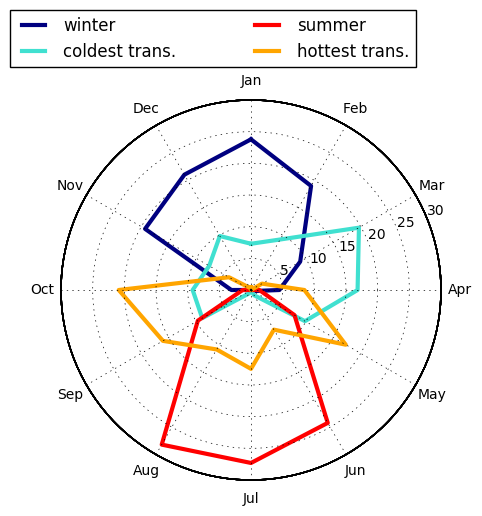
\includegraphics[scale=0.65]{Figures/Monthly_distribution.jpg}
  \caption{Monthly distribution for clusters: \textit{summer, winter, hottest and coldest transition}. $S_{vector}$ contains variables outdoor temperature, weather temperature and sunshine presence.}
  \label{fig:monthly}
\end{figure} 


Something to note is how the spring and autumn period share some patterns in common, this is the case when the \textit{hottest transition} appears in May or when the \textit{coldest transition} appears in October for instance. Other interesting aspects is how the coldest and hottest transitions remain inside of the winter and summer period respectively. One can also see how these clusters are distributed in a daily fashion in Figure \ref{fig:daily}, one observes that each cluster is distributed in an equitable fashion over \textbf{a)} working days, weekends and holidays; and \textbf{b)} the days of the week in general.   

\begin{figure}[h!]
  \vspace{0.5em} %better style
  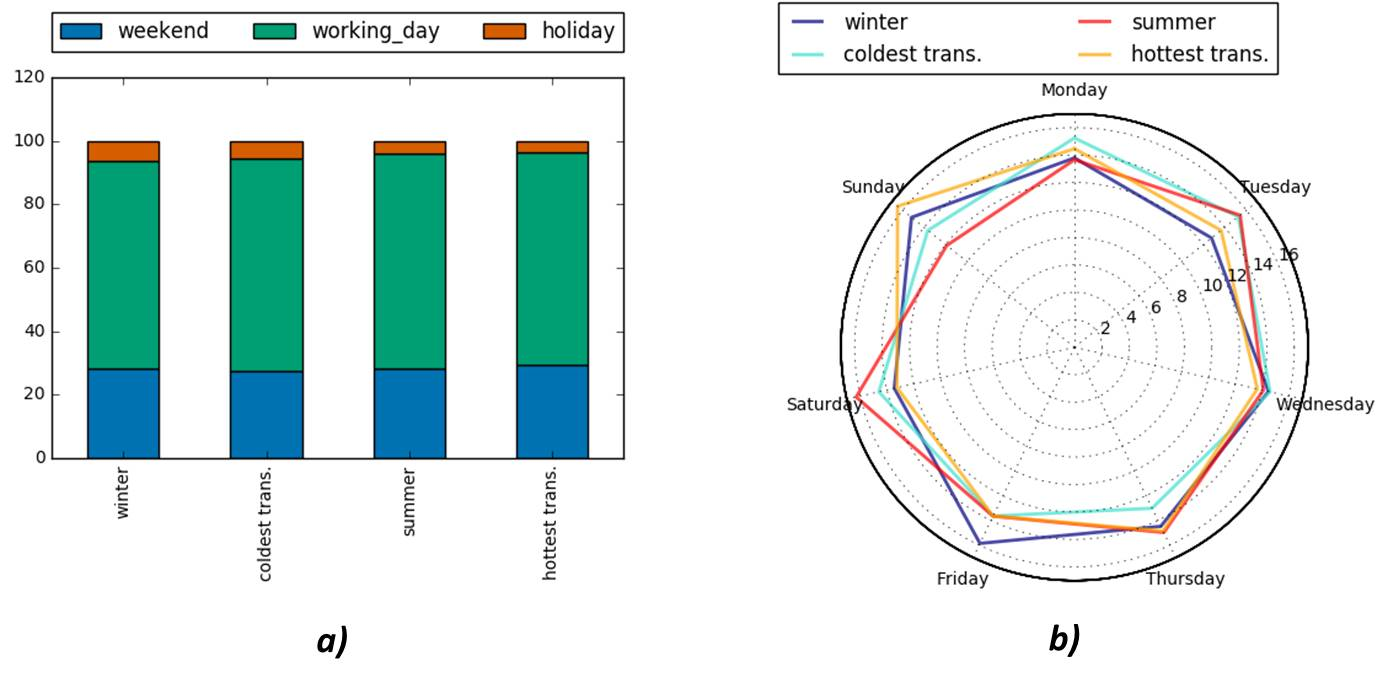
\includegraphics[scale=0.65]{Figures/daily_distribution_season.jpg}
  \caption{Monthly distribution for clusters: \textit{summer, winter, hottest and coldest transition}. $S_{vector}$ contains variables outdoor temperature, weather temperature and sunshine presence.}
  \label{fig:daily}
\end{figure} 

Finally, a calendar visualization is proposed to see the distribution of these clusters. Annex \ref{fig:s_vector_temperature} contains a calendar visualization for \textbf{a)} $S_{vector}$ using outdoor temperature and weather temperature; and \textbf{b)} $S_{vector}$ using outdoor temperature, weather temperature and sunshine presence. The sunshine presence variable affects the clustering such that they become more heterogeneous and blended being in this way a more representative abstraction of the weather nature.  

\begin{figure}[h!]
  \vspace{0.5em} %better style
  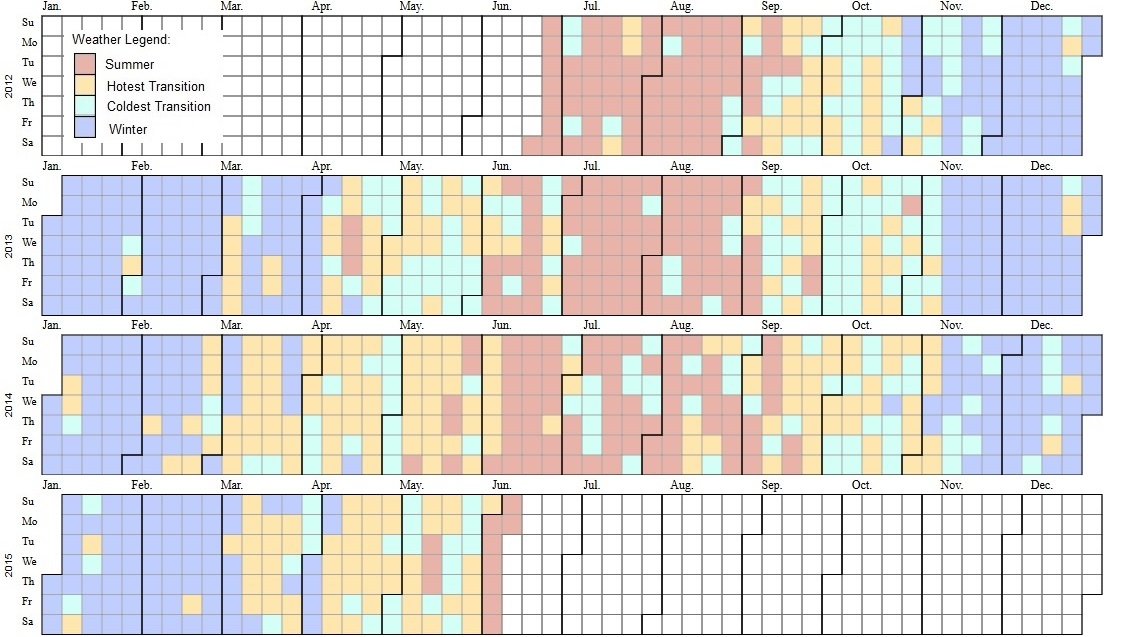
\includegraphics[scale=0.45]{Figures/temperatures.jpg}
  \caption{\textbf{a)} Daily representation of clusters: \textit{summer, winter, coldest and hottest transition} using a $S_{vector}$ with outdoor temperature and weather temperature.}
  \label{fig:s_vector_temperature}
\end{figure}

\begin{figure}[h!]
  \vspace{0.5em} %better style
  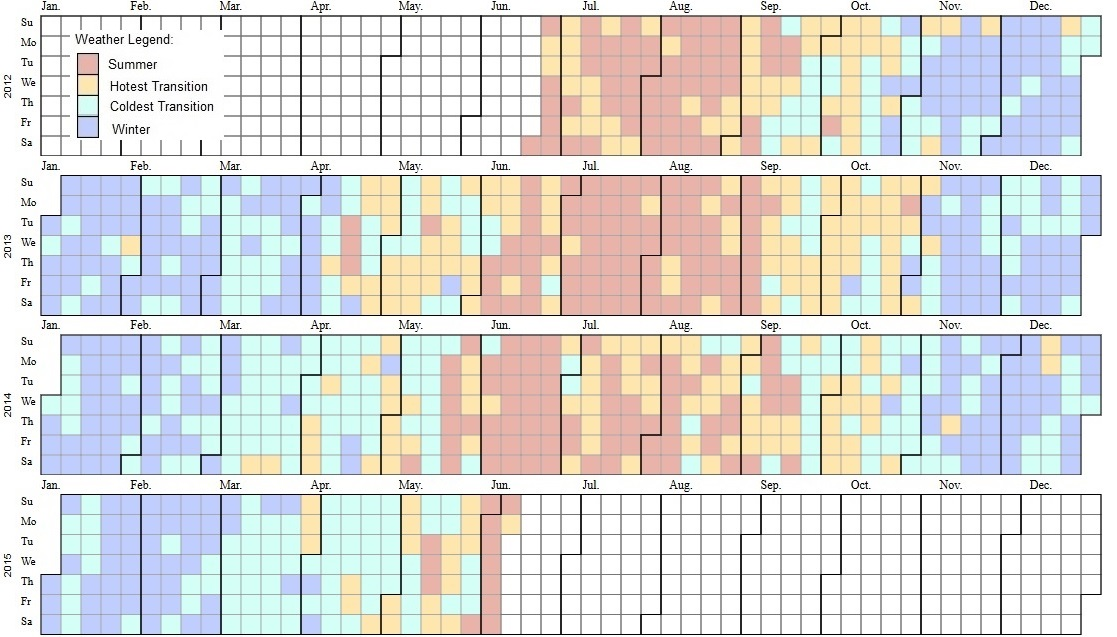
\includegraphics[scale=0.45]{Figures/sushine.jpg}
  \caption{\textbf{b)} Daily representation of clusters: \textit{summer, winter, coldest and hottest transition} using a $S_{vector}$ with outdoor temperature, weather temperature and sunshine presence variables.}
  \label{fig:s_vector_sunshine}
\end{figure}




%--------------------------------------------------------------------------------------
\subsection{Results of the GaHMM interactional model}
\label{sec:interactional_results}

As it was exposed in section \ref{sec:interactional_evaluation}, three clusters were found by using the best \textit{GaHMM} interactional model. In this model, the $R_{vector}$ represents the existing correlation between categories \textit{[A\_3, A\_{4\_1}, A\_{4\_2},  A\_{6\_1}, A\_{6\_2}]} and the $CO_2$ levels of the North-East part of the building. Following this idea, \textbf{Regimen of Negative Correlation} contains a collection of days where the negative correlation in the $R_{vector}$ is relevant. \textbf{Regimen of Weak Correlation} contains a collection of days where there is a weak linear correlation in the $R_{vector}$, and finally, \textbf{Regimen of Positive Correlation} contains a collection of days where \textbf{$R_{vector}$} has mostly positive correlation. Each center of the cluster is represented by the mean vector and a standard deviation (see table \ref{tab:regimen_centers}). For example, one reads that the $CO_2$ levels has, in average, a correlation of -0.6 with the angles of the North exterior blinds in Regimen of Negative Correlation.

% Table generated by Excel2LaTeX from sheet 'Hoja1'
\begin{table}[htbp]
  \centering
  \tiny
  \caption{Center vector of clusters: \textit{[Regimen of Negative Correlation, Positive Correlation and Weak correlation]} with their correspondent standard deviation.}
    \begin{tabular}{|l|c|c|c|c|c|}
    \multicolumn{6}{c}{\textcolor[rgb]{ .31,  .506,  .741}{\textbf{Regimen of Negative Correlation}}} \bigstrut[b]\\
    \hline
    \textbf{CO2 vs.} & \multicolumn{1}{l|}{\textbf{Blinds angle N Out}} & \multicolumn{1}{l|}{\textbf{ Blinds angle N In}} & \multicolumn{1}{l|}{\textbf{ Blinds angle E Out}} & \multicolumn{1}{l|}{\textbf{Blinds angle E In}} & \multicolumn{1}{l|}{\textbf{Blinds height N Out}} \bigstrut\\
    \hline
    \textit{mean\_vector} & -0.60 & -0.50 & -0.50 & -0.60 & -0.60 \bigstrut\\
    \hline
    \textit{std} & 0.10 & 0.17 & 0.14 & 0.10 & 0.10 \bigstrut\\
    \hline
    \textbf{CO2 vs.} & \multicolumn{1}{l|}{\textbf{Blinds height N In}} & \multicolumn{1}{l|}{\textbf{ Blinds height E Out}} & \multicolumn{1}{l|}{\textbf{Blinds height E In}} & \multicolumn{1}{l|}{\textbf{Temp. Vent. NE Out}} & \multicolumn{1}{l|}{\textbf{Temp. Vent. NE In}} \bigstrut\\
    \hline
    \textit{mean} & -0.60 & -0.10 & -0.30 & 0.70 & 0.10 \bigstrut\\
    \hline
    \textit{std} & 0.10 & 0.37 & 0.22 & 0.20 & 0.50 \bigstrut\\
    \hline
    \multicolumn{1}{l}{} & \multicolumn{1}{c}{} & \multicolumn{1}{c}{} & \multicolumn{1}{c}{} & \multicolumn{1}{c}{} & \multicolumn{1}{c}{} \bigstrut[t]\\
    \multicolumn{6}{c}{\textcolor[rgb]{ .31,  .506,  .741}{\textbf{Regimen of Positive Correlation}}} \bigstrut[b]\\
    \hline
    \textbf{CO2 vs.} & \multicolumn{1}{l|}{\textbf{Blinds angle N Out}} & \multicolumn{1}{l|}{\textbf{ Blinds angle N In}} & \multicolumn{1}{l|}{\textbf{ Blinds angle E Out}} & \multicolumn{1}{l|}{\textbf{Blinds angle E In}} & \multicolumn{1}{l|}{\textbf{Blinds height N Out}} \bigstrut\\
    \hline
    \textit{mean} & 0.50 & 0.50 & 0.50 & 0.50 & 0.50 \bigstrut\\
    \hline
    \textit{std} & 0.20 & 0.20 & 0.17 & 0.20 & 0.20 \bigstrut\\
    \hline
    \textbf{CO2 vs.} & \multicolumn{1}{l|}{\textbf{Blinds height N In}} & \multicolumn{1}{l|}{\textbf{ Blinds height E Out}} & \multicolumn{1}{l|}{\textbf{Blinds height E In}} & \multicolumn{1}{l|}{\textbf{Temp. Vent. NE Out}} & \multicolumn{1}{l|}{\textbf{Temp. Vent. NE In}} \bigstrut\\
    \hline
    \textit{mean} & 0.50 & 0.40 & 0.50 & 0.40 & 0.30 \bigstrut\\
    \hline
    \textit{std} & 0.20 & 0.22 & 0.17 & 0.62 & 0.67 \bigstrut\\
    \hline
    \multicolumn{1}{l}{} & \multicolumn{1}{c}{} & \multicolumn{1}{c}{} & \multicolumn{1}{c}{} & \multicolumn{1}{c}{} & \multicolumn{1}{c}{} \bigstrut[t]\\
    \multicolumn{6}{c}{\textcolor[rgb]{ .31,  .506,  .741}{\textbf{Regimen of Weak Correlation}}} \bigstrut[b]\\
    \hline
    \textbf{CO2 vs.} & \multicolumn{1}{l|}{Blinds angle N Out} & \multicolumn{1}{l|}{ Blinds angle N In} & \multicolumn{1}{l|}{ Blinds angle E Out} & \multicolumn{1}{l|}{Blinds angle E In} & \multicolumn{1}{l|}{Blinds height N Out} \bigstrut\\
    \hline
    mean & -0.10 & 0.00 & -0.20 & -0.10 & -0.10 \bigstrut\\
    \hline
    std & 0.00 & 0.00 & 0.00 & 0.00 & 0.00 \bigstrut\\
    \hline
    \textbf{CO2 vs.} & \multicolumn{1}{l|}{Blinds height N In} & \multicolumn{1}{l|}{ Blinds height E Out} & \multicolumn{1}{l|}{Blinds height E In} & \multicolumn{1}{l|}{Temp. Vent. NE Out} & \multicolumn{1}{l|}{Temp. Vent. NE In} \bigstrut\\
    \hline
    \textit{mean} & -0.10 & 0.10 & -0.10 & 0.20 & 0.30 \bigstrut\\
    \hline
    \textit{std} & 0    & 0    & 0    & 0    & 0 \bigstrut\\
    \hline
    \end{tabular}%
  \label{tab:regimen_centers}%
\end{table}%

Clusters of Regimen of Negative, Weak and Positive correlation are distributed over the complete timeline (i.e. 1801 days) in the following respective manner $63.8\%, 28.2\%, 8\%$. Each cluster has a dominant component (see figure \ref{fig:daily_distribution} and \ref{fig:r_distribution}). For example, the regimen of Negative correlation is formed by 631 ($93.07\%$) working days, 26 ($3.83\%$) weekend days and 21 ($3.10\%$) holidays. Clearly, this cluster describes the interrelation of variables when there is occupant presence. In contrast, the regimen of Weak Correlation has a dominant component of weekend days (199 days) where generally there is absence of occupant presence. Thus one can associate a weak correlation with absence of occupants. However, there are cases where the correlation is weak, even if there are occupants present \footnote{Occupant presence assumed because the $CO_2$ levels follows the typical profile $ ID=[12, 15, 16] $ annex \ref{cluster_profiles}, for instance.}, this is the yellow area in figure \ref{fig:r_distribution}. \\

We conclude a weak correlation implies absence of occupants but at the same time is an indicative (in the case when there is actual occupant presence) of an atypical interaction of variables, that could involve cases where the blinds are not at all used during the day (totally closed for instance) or the exhaust air temperature stays static during the entire day, or other atypical situations (it could imply sensor faults). Unfortunately, we do not have a ground truth information for these nonconforming days, and therefore we cannot corroborate this hypothesis. Nevertheless when one sees the details of this cluster, one observes time periods where the correlation is weak for business days. One example, is the period of \textit{Friday November $8^{th}$, 2013} to \textit{Tuesday November $12^{th}$, 2013} that presents frozen data in all the variables of the dataset (see figure \ref{fig:maintenance}). We suppose it corresponds to a building maintenance period. Finally, the Positive correlation has a dominant component of Saturdays, this correspond to days where the $CO_2$ levels were accumulated until Friday ($CO_2$ levels in the range of 800 ppm at midnight), and on Saturday the $CO_2$ levels diminish during the day (see profile $ID=26$, annex \ref{cluster_profiles}). All the information in this section is used in the case study in section \ref{section:case_study_1}. 

\begin{figure}[h!]
  \vspace{0.5em} %better style
  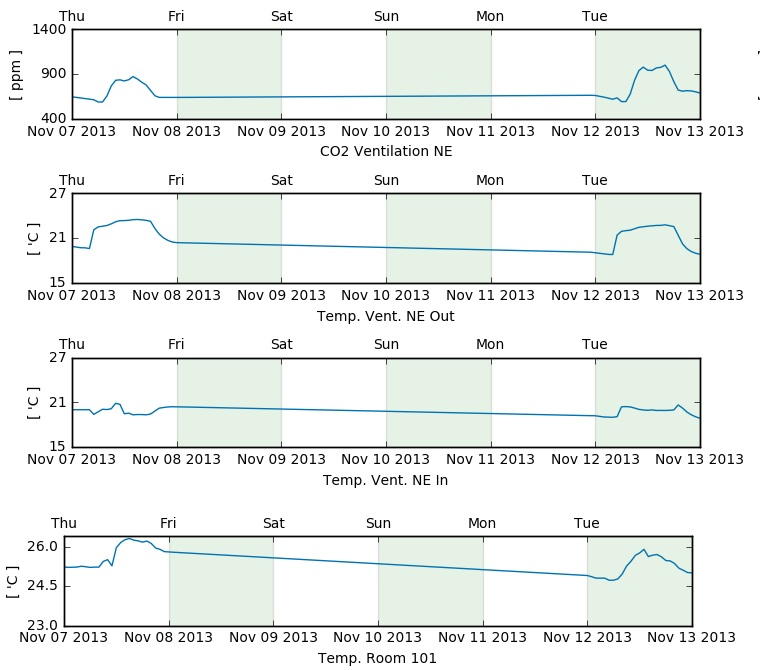
\includegraphics[scale=0.65]{Figures/maintenance_period.jpg}
  \caption{Discovered building maintenance period: frozen data in all the variables of the dataset.}
  \label{fig:maintenance}
\end{figure}



\begin{figure}[h!]
  \vspace{0.5em} %better style
  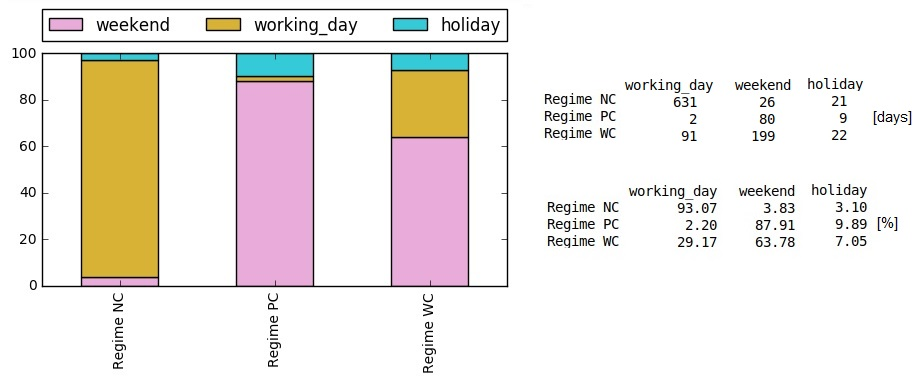
\includegraphics[scale=0.65]{Figures/Distribution_daily.jpg}
  \caption{Distribution for clusters: \textit{Regimen of Negative, Weak and Positive correlation} over working days, weekends and holidays.}
  \label{fig:daily_distribution}
\end{figure}


\begin{figure}[h!]
  \vspace{0.5em} %better style
  \includegraphics[scale=0.65]{Figures/Interactional_cluster_daily_distribution.jpg}
  \caption{Distribution for clusters: \textit{Regimen of Negative, Weak and Positive correlation} over working days, weekends and holidays.}
  \label{fig:r_distribution}
\end{figure}


%--------------------------------------------------------------------------------------
\subsection{Results of the GaHMM profile model}
\label{sec:profile_results}

Each variable has his own \textit{GaHMM profile model} and their results are in the digital folder annex: \textit{iPythonBooks/Diversity of profiles}. To exemplify the results of the \textit{GaHMM profile} model, we propose to use the $CO_2$ levels of the building. For this purpose, we firstly briefly review topics related with indoor air quality (IAQ), and secondly, a proposition for spotting discord profiles is presented by using the \textit{GaHMM profile} model in combination with the hierarchical agglomerative clustering. Finally, the results and methodology are applied in a study case in section \ref{section:case_study_1}  

\subsubsection{Analysis of the Carbon Dioxide $CO_2$ measurement in the Building}
\label{section:CO2_analysis}

One way to evaluate the IAQ of buildings is by using $CO_2$ sensors in these facilities. This measurement as well as other indicators (e.g. volatile organic component (TVOC), nitrogen dioxide $NO_2$, etc.) have helped researches to find health problems related to poor air quality for at least the two last decades (\citeauthor{persily1997evaluating}, \citeyear{persily1997evaluating})\cite{persily1997evaluating}, (\citeauthor{lee2000indoor}, \citeyear{lee2000indoor})\cite{lee2000indoor} (\citeauthor{erdmann2002indoor}, \citeyear{erdmann2002indoor}) \cite{erdmann2002indoor}. Carbon dioxide is not generally considered to be a health concern at the concentrations that typically occur indoors \cite{persily1997evaluating}, however new studies show that constant exposure to poor indoor environments affects health, and that some illness (e.g. allergy and asthma symptoms, and respiratory illnesses) are directly associated to the IAQ \cite{erdmann2002indoor}). Most of the HVAC systems re-circulate the indoor air to maintain the thermal comfort and reduce cost the of operations of cooling and heating (\citeauthor{prill2000measure}, \citeyear{prill2000measure})\cite{prill2000measure}. This operational strategy and the nature of $CO_2$ have a cumulative effect on the indoor air quality with time lags (\citeauthor{dong2010information},\citeyear{dong2010information}) \cite{dong2010information}.  

Understanding the typical pattern of fluctuation of this variable during the day will provide important information to the stakeholders so that designers can create an objective air ventilation system assessment, based on the typical fluctuations of the $CO_2$ levels. For example, a designer might know whether the indoor contaminants depend only on the occupants or there are other sources of contamination that affect the air quality such as the emissions from building and furnishing material, the intake of outdoor contaminants \cite{persily1997evaluating}, the effects of heating/cooling operations, maintenance operations, etc. We believe that the analysis of the "typical pattern of fluctuation" of the $CO_2$ levels can be done by finding the motif and discord profiles.

\paragraph{Motif and discord profiles for the $CO_2$ variable:}
\label{motif_results}

This section discuses the motif and discord profiles for $CO_2$ measurement of the North-East and South-West zones of the building. The selection of these profiles follows the established criteria of the technical community involved in indoor air quality evaluation and is a benchmarking between the North-East and South-West ventilation system.


\subparagraph{\textit{Indoor air quality evaluation using Carbon Dioxide ($CO_2$) measurement}}


It is widely reported by specialists that ASHRAE recommends $CO_2$ concentrations be below 1800 $mg/m^{3}$ (1000
ppm(v)) \cite{persily1997evaluating,erdmann2002indoor, lee2000indoor}. ASHRAE standard 62-2001 \cite{standard2001standard} in his table 6.1 presents the minimum ventilation rates for office buildings, that is 5-15 $cfm/person$ depending on the building zone and the people outdoor air rate \footnote{\textbf{People Outdoor Air Rate}: The outdoor airflow rate per person should be provided in the breathing zone to dilute contaminants that are emitted at a rate that is related more to population than to floor area}. The relationship between $CO_2$ concentrations and indoor air quality is directly affected by the rate at which people generate $CO_2$ and the capacity of the ventilation
system to dilute indoor air pollutants \cite{persily1997evaluating}. The $CO_2$ rate generated by occupants depends highly on their physical activity and physical condition; if the ventilation system is not able to dilute CO2 levels slightly over 1000 ppm this is not considered as a health risk but is considered as an uncomfortable situation because of the body odors that occupants can perceive \cite{persily1997evaluating,prill2000measure}.


The differential between indoor and outdoor levels of $d_{CO_2} = 700 ppm(v)$ (i.e. $\approx$ 1000 - 300 ppm ) is a measure of acceptability with respect to body odor. We could say, if the differential between indoor and outdoor levels of $CO_2$ is lower than 700 ppm, 80\% of building’s visitors will find the odors at an acceptable level, independent of the outdoor levels of $CO_2$ \cite{persily1997evaluating}. Thus, a threshold of approximately $1000 \ ppm$ is a limit that helps us to identify unwanted daily profiles. However, what happens with differential $CO_2$ lower than 700 ppm? Recent studies have indicated that even peaks of concentration below 1000 ppm are associated with an increased prevalence of certain afflictions of the mucous membranes, some respiratory problems, perceptions of stuffiness, discomfort and irritation \cite{persily1997evaluating,erdmann2002indoor}. 


Therefore, we cannot not say that levels lower than 1000 ppm are necessarily healthy, especially if there are $CO_2$ emanation peaks. One can find in literature sophisticated ways of evaluating air quality, for example by using the $CO_2$ outdoor levels \cite{persily1997evaluating} or estimating occupancy profiles for checking the correct ventilation rates \cite{batterman2017review}. In our case, since we only possess the indoor $CO_2$ levels, we only consider two types of discords that allow us to check the IAQ: \textit{1.} profiles where the CO2 level are higher than 1000 ppm and \textit{2.} profiles that do not follow the normal pattern of fluctuation of the CO2 variable. The latter is explained in the next section.

\subparagraph{\textit{Benchmarking between the North-East and South-West ventilation system}} 
\label{sec:discord_finding}


Here we propose a comparative analysis between the North-East and South-West ventilation system of the building using our approach, that is the \textit{GaHMM-profile} model for the time series of measurement of $CO_2$ and a hierarchical agglomerative clustering. Our final goal is to find the most common daily profiles (i.e. \textit{motifs}) and potential anomalous daily profiles (i.e. \textit{discords}) that are present in both ventilation systems. To explain how we proceeded, we give outline of the 4 steps to follow with each step afterwards being explained in detail\footnote{The script code of this procedure is in files: \textit{ iPythonBooks/Diversity of profiles/.. and  iPythonBooks/Cases of study/Comparison ventilation System NE vs SW.ipynb}}: \textbf{a)} once the GaHMM-profile models for the $CO_2$ variables are trained according to what is explained in the section \ref{sec:profile_model}. We select one GaHMM-profile model at a time and build a matrix of observations $M$ using the cluster profiles of each specific GaHMM-profile model. \textbf{ b)} We use hierarchical agglomerative clustering algorithms \cite{mullner2011modern} to group our cluster profiles\footnote{It is important to recall that our clusters are defined by two vectors: a mean vector and a standard deviation vector of length equal to 24, each value for each hour of the day, therefore, mean vector: $P_x = \{ \mu_{x_i} \forall i \in [0,23] \}$  and standard deviation vector: $STD_x = \{ \sigma_{x_i} \forall i \in [0,23] \}$} into the observation matrix $M$. \textbf{c)} Once the hierarchical agglomerative clustering is done, we use the cophenetic correlation \cite{saraccli2013comparison} to guarantee that the metrics and methods that were used for the hierarchical clustering were the correct ones and therefore the resulting dendrogram preserves the pairwise distances between the original profiles \cite{saraccli2013comparison}. \textbf{d)} After the correct selection of methods and metrics, we propose the selection of the discords and motifs profiles by using a dendrogram and fixing a cut-off value as a threshold. \\

\textit{Step a)} We select a GaHMM-profile that corresponds to the variable of our interest (i.e. \textit{V005\_vent01\_CO2 model} for North-East and \textit{V022\_vent02\_CO2 model} for South-West). Afterwards, we compile all the cluster profiles that belong to this GaHMM-profile model (see appendix
\ref{fig:candidates_profiles_NE}). For this purpose, as is mentioned in section \ref{sec:profile_model} using the \textit{HMM} library \cite{gahmm_manual}, one can access to each profile by using his respective number of identification ID. For example: $model.means\_[0]$ returns the mean vector that correspond to profile $ID = 0$. We list all mean vectors for all clusters, and we construct a matrix $M$ of size $N_p \times 24$ where $N_p$ is the number of cluster profiles that belong to the GaHMM-profile model. This matrix is known as the observation matrix $M$. \\


\textit{Step b)} Once the matrix $M$ is done, we use the clustering package of SciPy \footnote{Hierarchical clustering package can be found on  \url{https://docs.scipy.org/doc/scipy-0.14.0/reference/cluster.hierarchy.html\#module-scipy.cluster.hierarchy}} for performing the hierarchical agglomerative clustering. We follow the theory and indications provided by \citeauthor{mullner2011modern} and \citeauthor{saraccli2013comparison}'s work \cite{mullner2011modern,saraccli2013comparison}. The linkage routine \footnote{Linkage Method can be found on \url{https://docs.scipy.org/doc/scipy-0.14.0/reference/generated/scipy.cluster.hierarchy.linkage.html\#scipy.cluster.hierarchy.linkage} } is applied over the observation matrix using different methods and metrics as it is suggested by \citeauthor{saraccli2013comparison}'s work \cite{saraccli2013comparison}. \\  


\textit{Step c)} One important aspect in hierarchical agglomerative clustering, is the faithful representation of two or more merged clusters. That is, when we merge two clusters, we would like that the resulting cluster to conserve relevant aspects of the two cluster that were merged \cite{saraccli2013comparison}. We
can measure this desired effect by using the cophenetic correlation coefficient \footnote{Cophenetic correlation coefficient: is a measure of how faithfully a dendrogram preserves the pairwise distances between the original unmodeled data points \cite{saraccli2013comparison}}, the closer this measure is to 1, the better preservation of pairwise distance between the original cluster profiles we get.\\  


% Table generated by Excel2LaTeX from sheet 'cophenetic correlation'
\begin{table}[htbp]
  \centering
  \scriptsize
  \caption{The cophenetic correlation values for the hierarchical clustering of: a) $CO_2$ cluster profiles for the North-East ventilation system b) $CO_2$ cluster profiles for the South-West ventilation system, using different distance metrics and linkage methods.}
       \begin{tabular}{|l|r|r|r|r|}
    \hline
    \multicolumn{5}{|c|}{a) North-East ventialtion system (V005\_vent01\_CO2)} \bigstrut\\
    \hline
    \rowcolor[rgb]{ .851,  .851,  .851} \textit{\textbf{linkage methods}} & \multicolumn{4}{c|}{\cellcolor[rgb]{ .855,  .933,  .953} \textit{\textbf{distance metrics}}} \bigstrut\\
\cline{2-5}    \rowcolor[rgb]{ .851,  .851,  .851}      & \multicolumn{1}{c|}{\cellcolor[rgb]{ .855,  .933,  .953} \textit{\textbf{euclidean}}} & \multicolumn{1}{c|}{\cellcolor[rgb]{ .855,  .933,  .953} \textit{\textbf{minkowski}}} & \multicolumn{1}{c|}{\cellcolor[rgb]{ .855,  .933,  .953} \textit{\textbf{cityblock}}} & \multicolumn{1}{c|}{\cellcolor[rgb]{ .855,  .933,  .953} \textit{\textbf{sqeuclidean}}} \bigstrut\\
    \hline
    \rowcolor[rgb]{ .851,  .851,  .851} \textit{\textbf{average}} & \cellcolor[rgb]{ .573,  .816,  .314} \textbf{0.76324} & \cellcolor[rgb]{ 1,  1,  1} 0.76324 & \cellcolor[rgb]{ 1,  1,  1} 0.74766 & \cellcolor[rgb]{ 1,  1,  1} 0.73534 \bigstrut\\
    \hline
    \rowcolor[rgb]{ .851,  .851,  .851} \textit{\textbf{single}} & \cellcolor[rgb]{ 1,  1,  1} 0.58851 & \cellcolor[rgb]{ 1,  1,  1} 0.58851 & \cellcolor[rgb]{ 1,  1,  1} 0.65695 & \cellcolor[rgb]{ 1,  1,  1} 0.50559 \bigstrut\\
    \hline
    \rowcolor[rgb]{ .851,  .851,  .851} \textit{\textbf{complete}} & \cellcolor[rgb]{ 1,  1,  1} 0.55127 & \cellcolor[rgb]{ 1,  1,  1} 0.55127 & \cellcolor[rgb]{ 1,  1,  1} 0.66504 & \cellcolor[rgb]{ 1,  1,  1} 0.50986 \bigstrut\\
    \hline
    \rowcolor[rgb]{ .851,  .851,  .851} \textit{\textbf{median}} & \cellcolor[rgb]{ 1,  1,  1} 0.72623 & \multicolumn{1}{l|}{\cellcolor[rgb]{ 1,  1,  1} -} & \multicolumn{1}{l|}{\cellcolor[rgb]{ 1,  1,  1} -} & \multicolumn{1}{l|}{\cellcolor[rgb]{ 1,  1,  1} -} \bigstrut\\
    \hline
    \rowcolor[rgb]{ .851,  .851,  .851} \textit{\textbf{ward}} & \cellcolor[rgb]{ 1,  1,  1} 0.65094 & \multicolumn{1}{l|}{\cellcolor[rgb]{ 1,  1,  1} -} & \multicolumn{1}{l|}{\cellcolor[rgb]{ 1,  1,  1} -} & \multicolumn{1}{l|}{\cellcolor[rgb]{ 1,  1,  1} -} \bigstrut\\
    \hline
    \rowcolor[rgb]{ .851,  .851,  .851} \textit{\textbf{weighted}} & \cellcolor[rgb]{ 1,  1,  1} 0.73530 & \cellcolor[rgb]{ 1,  1,  1} 0.73530 & \cellcolor[rgb]{ 1,  1,  1} 0.57468 & \cellcolor[rgb]{ 1,  1,  1} 0.59748 \bigstrut\\
    \hline
    \multicolumn{1}{r}{} & \multicolumn{1}{r}{} & \multicolumn{1}{r}{} & \multicolumn{1}{r}{} & \multicolumn{1}{r}{} \bigstrut\\
    \hline
    \multicolumn{5}{|c|}{b) South-West ventilation system (V022\_vent02\_CO2)} \bigstrut\\
    \hline
    \rowcolor[rgb]{ .851,  .851,  .851} \textit{\textbf{linkage methods}} & \multicolumn{4}{c|}{\cellcolor[rgb]{ .855,  .933,  .953} \textit{\textbf{distance metrics}}} \bigstrut\\
\cline{2-5}    \rowcolor[rgb]{ .851,  .851,  .851}      & \multicolumn{1}{c|}{\cellcolor[rgb]{ .855,  .933,  .953} \textit{\textbf{euclidean}}} & \multicolumn{1}{c|}{\cellcolor[rgb]{ .855,  .933,  .953} \textit{\textbf{minkowski}}} & \multicolumn{1}{c|}{\cellcolor[rgb]{ .855,  .933,  .953} \textit{\textbf{cityblock}}} & \multicolumn{1}{c|}{\cellcolor[rgb]{ .855,  .933,  .953} \textit{\textbf{sqeuclidean}}} \bigstrut\\
    \hline
    \rowcolor[rgb]{ .851,  .851,  .851} \textit{\textbf{average}} & \cellcolor[rgb]{ .573,  .816,  .314} \textbf{0.74394} & \cellcolor[rgb]{ 1,  1,  1} 0.74394 & \cellcolor[rgb]{ 1,  1,  1} 0.69358 & \cellcolor[rgb]{ 1,  1,  1} 0.72524 \bigstrut\\
    \hline
    \rowcolor[rgb]{ .851,  .851,  .851} \textit{\textbf{single}} & \cellcolor[rgb]{ 1,  1,  1} 0.68275 & \cellcolor[rgb]{ 1,  1,  1} 0.68275 & \cellcolor[rgb]{ 1,  1,  1} 0.70526 & \cellcolor[rgb]{ 1,  1,  1} 0.68563 \bigstrut\\
    \hline
    \rowcolor[rgb]{ .851,  .851,  .851} \textit{\textbf{complete}} & \cellcolor[rgb]{ 1,  1,  1} 0.59179 & \cellcolor[rgb]{ 1,  1,  1} 0.59179 & \cellcolor[rgb]{ 1,  1,  1} 0.57658 & \cellcolor[rgb]{ 1,  1,  1} 0.55841 \bigstrut\\
    \hline
    \rowcolor[rgb]{ .851,  .851,  .851} \textit{\textbf{median}} & \cellcolor[rgb]{ 1,  1,  1} 0.69560 & \multicolumn{1}{l|}{\cellcolor[rgb]{ 1,  1,  1} -} & \multicolumn{1}{l|}{\cellcolor[rgb]{ 1,  1,  1} -} & \multicolumn{1}{l|}{\cellcolor[rgb]{ 1,  1,  1} -} \bigstrut\\
    \hline
    \rowcolor[rgb]{ .851,  .851,  .851} \textit{\textbf{ward}} & \cellcolor[rgb]{ 1,  1,  1} 0.60313 & \multicolumn{1}{l|}{\cellcolor[rgb]{ 1,  1,  1} -} & \multicolumn{1}{l|}{\cellcolor[rgb]{ 1,  1,  1} -} & \multicolumn{1}{l|}{\cellcolor[rgb]{ 1,  1,  1} -} \bigstrut\\
    \hline
    \rowcolor[rgb]{ .851,  .851,  .851} \textit{\textbf{weighted}} & \cellcolor[rgb]{ 1,  1,  1} 0.60343 & \cellcolor[rgb]{ 1,  1,  1} 0.60343 & \cellcolor[rgb]{ 1,  1,  1} 0.60422 & \cellcolor[rgb]{ 1,  1,  1} 0.71199 \bigstrut\\
    \hline
    \end{tabular}%
  \label{tab:cophenetic_correlation}%
\end{table}%


We cluster the observation matrix $M$ by using the distance metrics: \textit{[euclidean, minkowski, cityblock, sqeuclidean]} and the linkage methods: \textit{[average, single, complete, median, ward, weighted}] \citep{saraccli2013comparison} and, we evaluate the quality of the hierarchical clustering by using the cophenetic correlation. The result of this evaluation is in table \ref{tab:cophenetic_correlation} where we observe that the \textit{average linkage method} and metrics \textit{euclidean distance, minkowski distance} have the best cophenetic correlation \footnote{Since euclidean distance and minkowski distance achieve the same result, in this work the euclidean distance is used due to his simplicity.}. \\ 


 
\begin{figure}[h!]
  \vspace{0.5em} %better style
  \includegraphics[scale=0.65]{Figures/dendrogram_CO2_NE.jpg}
  \caption{ Extract of the resulting hierarchical clustering dendrogram for the observed matrix $M$ using the $CO_2$ cluster profiles of the North-East ventilation system.}
  \label{fig:dendrogram_CO2_NE}
\end{figure} 

\textit{Step d)} The resulting dendrogram of the hierarchical clustering can be obtained by using the dendrogram's plot method of the clustering package of SciPy \footnote{Dendrogram method available on: \url{https://docs.scipy.org/doc/scipy-0.14.0/reference/generated/scipy.cluster.hierarchy.dendrogram.html}}. Figure \ref{fig:dendrogram_CO2_NE} shows an extract of the resulting dendrogram for the $CO_2$ cluster profiles for the North-East ventilation system. We observe that the cluster profiles $ID_x = [33, 1, 9, 4, 25, 17, 22, 11, 27]$ are very similar to each other (Figure \ref{fig:CO2_candidates_comparison}), however this is not the case for the cluster profile $ID_y=29$. This fact is remarkable when we observe the similarity metric (i.e. euclidean distance using the average linkage method) between cluster $ID_y=29$ and any profile of $ID_x$. Based on this similarity metric, we can conclude that clusters of $ID_x$ do not match with $ID_y$ and therefore they are two different classes of patterns. Looking at the differences in profile $ID_y = 29$, we observe an abnormal fluctuation, that is, that the $CO_2$ levels are above $800 \ ppm$ at the very beginning of the day  which is contrary to the normal level $\approx [400 - 650] \ ppm$. Thus, we can conclude that clusters of $ID_x$ should be part of the motif clusters and clusters of $ID_y$ should be part of the discord clusters. 

\begin{figure}[h!]
  \vspace{0.5em} %better style
  \includegraphics[scale=0.5]{Figures/CO2_candidates_comparison.jpg}
  \caption{$CO_2$ cluster profiles \textit{$ID_x$ = [33, 1, 9, 4, 25, 17, 22, 11, 27]} for the North-East ventilation system.}
  \label{fig:CO2_candidates_comparison}
\end{figure}  

Heuristically, we define an euclidean distance of 300 as a cut-off limit in the resulting dendrograms for the two systems (\ref{fig:dendrogram_CO2_NE_complete}, \ref{fig:dendrogram_CO2_SW_complete}), this allows to discriminate the discord and motif profiles. The cut-off value creates 11 hierarchical clusters (\ref{tab:h_cluster_all}) in the hierarchical clustering dendrogram of the North-East ventilation system (annex \ref{fig:dendrogram_CO2_NE_complete}). One can observe that the clusters are joined together in a hierarchical fashion from the closest, that is most similar (i.e. shorter distance), to the furthest apart, that is the most different (i.e. larger distance). Those clusters that join other clusters at further distances over 300 are considered as discord clusters because they differ more than the average of clusters. These discord cluster profiles (i.e. \textit{[30, 3, 13, 18, 20, 10, 31, 29}) can be appreciated in annex \ref{fig:discord_candidates_all}. The same cut-off value was applied for the hierarchical clustering dendrogram of the $CO_2$ clusters of the South-West ventilation system (annex \ref{fig:dendrogram_CO2_SW_complete}). We found in this case 4 hierarchical clusters (\textit{[B1, B2, B3, B4]}) as is shown in table \ref{tab:h_cluster_all}. However, there is no clusters that join other clusters at distances greater than 300. Looking at all the clusters for the South-West system (\ref{fig:candidates_profiles_SW}) we observe that all of them follow an "uniform" pattern and there is no big difference at first glance. Nevertheless, we decided to spot those cluster profiles that diverge slightly from the rest of the clusters in the South-West ventilation system, so for that we created a new cut-off value of 200 and found clusters \textbf{ID=23, 28, 34} (see annex \ref{fig:discord_candidates_all_SW}). These clusters represent mostly high $CO_2$ levels on the winter period but this fluctuation is still close to the normal. One can observe therefore that a threshold between 200 and 300 is a good value for detecting abnormal fluctuations for both ventilation systems.  \\

% Table generated by Excel2LaTeX from sheet 'hierarchical clustering'
\begin{table}[htbp]
  \centering
  \scriptsize
  \caption{Hierarchical clustering for a) $CO_2$ clusters of the North-East ventilation system b) $CO_2$ clusters of the South-West ventilation system}
       \begin{tabular}{|l|l|l|rrr}
    \multicolumn{3}{c}{a) North-East ventilation system} &      & \multicolumn{2}{c}{b) South-West ventilation system} \bigstrut[b]\\
\cline{1-3}\cline{5-6}    \rowcolor[rgb]{ .851,  .851,  .851} \textbf{Observation} & \textbf{Hierarchical} & \multicolumn{1}{c|}{\textbf{V005\_vent01\_CO2 (CO2 levels)}} & \multicolumn{1}{r|}{\cellcolor[rgb]{ 1,  1,  1} } & \multicolumn{1}{l|}{\textbf{Hierarchical}} & \multicolumn{1}{c|}{\textbf{V022\_vent02\_CO2 (CO2 levels)}} \bigstrut[t]\\
    \rowcolor[rgb]{ .851,  .851,  .851}      & \textbf{Cluster ID} & \multicolumn{1}{c|}{\textbf{cluster ID}} & \multicolumn{1}{r|}{\cellcolor[rgb]{ 1,  1,  1} } & \multicolumn{1}{l|}{\textbf{cluster ID}} & \multicolumn{1}{c|}{\textbf{Cluster ID}} \bigstrut[b]\\
\cline{1-3}\cline{5-6}    motif & \cellcolor[rgb]{ .949,  .949,  .949} \textbf{A1 } & [2, 7, 21, 28]  & \multicolumn{1}{r|}{} & \multicolumn{1}{l|}{\cellcolor[rgb]{ .949,  .949,  .949} \textbf{B1}} & \multicolumn{1}{l|}{[4, 13, 28]} \bigstrut\\
\cline{1-3}\cline{5-6}    motif & \cellcolor[rgb]{ .949,  .949,  .949} \textbf{A2} & [6, 19, 26]  & \multicolumn{1}{r|}{} & \multicolumn{1}{l|}{\cellcolor[rgb]{ .949,  .949,  .949} \textbf{B2}} & \multicolumn{1}{l|}{[2, 6, 8, 14, 18, 21, 23, 24, 29, 31]} \bigstrut\\
\cline{1-3}\cline{5-6}    motif & \cellcolor[rgb]{ .949,  .949,  .949} \textbf{A3} & [0, 5, 8, 12, 14, 15, 16, 23, 24, 32]  & \multicolumn{1}{r|}{} & \multicolumn{1}{l|}{\cellcolor[rgb]{ .949,  .949,  .949} \textbf{B3}} & \multicolumn{1}{l|}{[0, 3, 10, 11, 17, 20, 25, 27, 34]} \bigstrut\\
\cline{1-3}\cline{5-6}    motif & \cellcolor[rgb]{ .949,  .949,  .949} \textbf{A4} & [1, 4, 9, 11, 17, 22, 25, 27, 33]  & \multicolumn{1}{r|}{} & \multicolumn{1}{l|}{\cellcolor[rgb]{ .949,  .949,  .949} \textbf{B4}} & \multicolumn{1}{l|}{[1, 5, 7, 9, 12, 15, 16, 19, 22, 26, 30, 32, 33]} \bigstrut\\
\cline{1-3}\cline{5-6}    discord & \cellcolor[rgb]{ .949,  .949,  .949} \textbf{A5} & [30]  &      &      &  \bigstrut\\
\cline{1-3}    discord & \cellcolor[rgb]{ .949,  .949,  .949} \textbf{A6} & [3]  &      &      &  \bigstrut\\
\cline{1-3}    discord & \cellcolor[rgb]{ .949,  .949,  .949} \textbf{A7} & [13]  &      &      &  \bigstrut\\
\cline{1-3}    discord & \cellcolor[rgb]{ .949,  .949,  .949} \textbf{A8} & [18]  &      &      &  \bigstrut\\
\cline{1-3}    discord & \cellcolor[rgb]{ .949,  .949,  .949} \textbf{A9} & [20]  &      &      &  \bigstrut\\
\cline{1-3}    discord & \cellcolor[rgb]{ .949,  .949,  .949} \textbf{A10} & [10, 31]  &      &      &  \bigstrut\\
\cline{1-3}    discord & \cellcolor[rgb]{ .949,  .949,  .949} \textbf{A11} & [29]  &      &      &  \bigstrut\\
\cline{1-3}    \end{tabular}%
  \label{tab:h_cluster_all}%
\end{table}%


We showed in this way, how our proposed approach \textit{GaHMM-profile model} in combination with the hierarchical agglomerative clustering allow us to identify potential discord clusters and motif clusters. \\


\subparagraph{\textit{Interpretation of the results}} 

As we can see on the resulting dendrograms [\ref{fig:dendrogram_CO2_NE_complete}, \ref{fig:dendrogram_CO2_SW_complete}] and the hierarchical agglomerative clustering table {\ref{tab:h_cluster_all}}, the tree dendrogram structure for the $CO_2$ clusters of the North-East ventilation system is not as homogeneous as the South-West ventilation system. This is because in the North-East ventilation system, there are some particular cluster profiles that behave very differently from the majority of the clusters. These particular clusters join the tree schema at a very latter level, and therefore, can be classified as discord profiles. We conclude that the North-East ventilation system suffered some kind of anomaly, because cluster profiles $ID=3; 13; 18; 20; 29; 30$ do not appear frequently and they show clearly a weird behavior that is not appropriated, and furthermore, they are not present on the South-West ventilation system. For example the cluster 18 starts the day with 800 ppm which is approximately 250 ppm more than the usual value ($\approx [450 - 650]$ ppm), this $CO_2$ level and the additional accumulation of $CO_2$ coming from the occupants provoked an excessive $CO_2$ level of over 1300 ppm in the afternoon. Another example is the cluster 13 that presents low levels at the beginning of the day, and then, the levels increase in an unexpected way, finishing the day with the highest levels of $CO_2$ very close to the threshold of $1000 \ ppm$. These kind of situations are not present on the South-West ventilation system where the maximum $CO_2$ level is not higher than 870 ppm. To verify this fact, is enough to check the daily profiles that belong to the clusters $ID = 28; 4; 13$ of the South-West ventilation system (annex \ref{fig:discord_candidates_all_SW}) since they have the highest $CO_2$ levels. Finally, the GaHMM-profile model allows us to spot 61 atypical days for the North-East ventilation system and 17 atypical days for the South-West ventilation system of a total of 1081 days. More details about the detected anomalies for the North-East system are exposed in the case study, in section \ref{section:case_study_1}  \\  


\subsection{Case study:  North-East ventilation system}

\label{section:case_study_1}

As pointed out in section \ref{section:CO2_analysis} the North East ventilation system presents some $CO_2$ anomalous profiles that were clustered as discord profiles (annex \ref{fig:discord_candidates_all}). In this section, we analyze in details these profiles and we show their linkage with other associated variables. To show this linkage, in a similar fashion to how we spotted motif and discord clusters for the $CO_2$ measurements, we use the individual \textit{GaHMM - profile} models and their correspondent hierarchical agglomerative clustering, for spotting discord cluster profiles. The variables used to do this analysis are: \textit{exhaust air temperature, intake air temperature, humidity of the exhausted air of the ventilation system, heating TABS comsuption (KWh) and temperature in rooms}. Each variable has his
own \textit{GaHMM profile model} and the respective hierarchical agglomerative dendrograms. The complete list of cluster profiles of each variable are included as a digital annex in directory: \textit{/Thesis\_project/iPythonBooks/Diversity of profiles}, and additionally, the hierarchical agglomerative dendrograms for each variable is in annexes \ref{fig:dendrogram_exhausted_NE}, \ref{fig:dendrogram_intake_NE}, \ref{fig:dendrogram_exhausted_humidity_NE}, \ref{fig:dendrogram_room_temperature_NE} and \ref{fig:dendrogram_heating_NE}. 


We use all our proposed models (i.e. \textit{GaHMM seasonal, interactional and profile models}) to construct a data frame with all the labels produced by each model. Table \ref{tab:data_frame} shows an example of how this data frame looks like\footnote{Labels \textit{t\_period\_1} and \textit{t\_period\_2} refers the \textit{hottest transition} and \textit{coldest transition} respectively.}. All of this information helps to spot atypical/typical cluster profiles across seasons, interactional regimen and years. One can use different filters according to the research interests. For example, one obtains the figure \ref{fig:winter_vs_summer} by using the filter "\textit{winter, regime NC and working days}". This bar plot describes the distribution of cluster profiles using the $ID_{profile}$ of three of the analyzed variables. In the first case, the $CO_2$ cluster profile $ID=32$ is the typical profile for working days in winter period, while the cluster profile $ID=8$ is the typical profile for summer period. Note that cluster profiles that exist in winter period do not necessarily appear in summer.     

% Table generated by Excel2LaTeX from sheet 'Hoja3'
\begin{table}[htbp]
  \centering
  \tiny
  \caption{DataFrame includes labels of interactional, seasonal and profile \textit{GaHMM models}. Each profile model is named using the name of the correspondent variable.}
    \begin{tabular}{|c|r|r|r|r|r|r|r|r|r|}
\cline{6-10}    \multicolumn{1}{r}{} & \multicolumn{1}{r}{} & \multicolumn{1}{r}{} & \multicolumn{1}{r}{} &      & \multicolumn{5}{c|}{GaHMM profile models (ID\_profile)} \bigstrut\\
    \hline
    \rowcolor[rgb]{ 1,  .753,  0} \multicolumn{1}{|l|}{\textbf{timestamp }} & \multicolumn{1}{l|}{\textbf{weekday}} & \multicolumn{1}{l|}{\textbf{day\_type }} & \multicolumn{1}{l|}{\textbf{interaction}} & \multicolumn{1}{l|}{\textbf{season }} & \multicolumn{1}{l|}{\textbf{V005\_}} & \multicolumn{1}{l|}{\textbf{V006\_vent01}} & \multicolumn{1}{l|}{\textbf{V012\_vent01}} & \multicolumn{1}{l|}{\textbf{V004\_vent01}} &  \bigstrut[t]\\
    \rowcolor[rgb]{ 1,  .753,  0}      &      &      & \multicolumn{1}{l|}{\textbf{label}} & \multicolumn{1}{l|}{\textbf{label}} & \multicolumn{1}{l|}{\textbf{vent01\_CO2 }} & \multicolumn{1}{l|}{\textbf{\_temp\_out }} & \multicolumn{1}{l|}{\textbf{\_temp\_in }} & \multicolumn{1}{l|}{\textbf{\_hum\_out }} & \multicolumn{1}{l|}{\textbf{…}} \bigstrut[b]\\
    \hline
    \multicolumn{1}{|r|}{23-Jun-12} & \multicolumn{1}{l|}{Saturday } & \multicolumn{1}{l|}{weekend } & \multicolumn{1}{l|}{Reg. PC } & \multicolumn{1}{l|}{summer } & 21   & 35   & 2    & 0    & \multicolumn{1}{l|}{\textbf{…}} \bigstrut\\
    \hline
    \multicolumn{1}{|r|}{24-Jun-12} & \multicolumn{1}{l|}{Sunday } & \multicolumn{1}{l|}{weekend } & \multicolumn{1}{l|}{Reg. WC } & \multicolumn{1}{l|}{summer } & 21   & 1    & 2    & 12   &  \bigstrut\\
    \hline
    \multicolumn{1}{|r|}{25-Jun-12} & \multicolumn{1}{l|}{Monday } & \multicolumn{1}{l|}{working\_day } & \multicolumn{1}{l|}{Reg. NC } & \multicolumn{1}{l|}{summer } & 8    & 11   & 3    & 33   &  \bigstrut\\
    \hline
    \multicolumn{1}{|r|}{26-Jun-12} & \multicolumn{1}{l|}{Tuesday } & \multicolumn{1}{l|}{working\_day } & \multicolumn{1}{l|}{Reg. NC } & \multicolumn{1}{l|}{summer } & 8    & 7    & 3    & 33   &  \bigstrut\\
    \hline
    …    &      &      &      &      &      &      &      &      &  \bigstrut\\
    \hline
    \end{tabular}%
  \label{tab:data_frame}%
\end{table}%


\begin{figure}[h!]
  \vspace{0.5em} %better style
  \includegraphics[scale=0.7]{Figures/cluster_dist_winter_summer.jpg}
  \caption{Distribution of cluster profiles (i.e. $ID_{profile}$) for working days: \textit{a)} winter period, b) summer period.}
  \label{fig:winter_vs_summer}
\end{figure} 

We use dendrograms: \ref{fig:dendrogram_exhausted_NE}, \ref{fig:dendrogram_intake_NE}, \ref{fig:dendrogram_exhausted_humidity_NE}, \ref{fig:dendrogram_room_temperature_NE} and \ref{fig:dendrogram_heating_NE} to spot the discord cluster profiles (i.e. the thick blue lines). At the end of the filter process, we discover a temporal coincidence of the discord profiles between variables. This is shown in a calendar visualization in figure \ref{fig:case-study}. 

Each small square represents a discord profile that was found by performing the process in section \ref{sec:discord_finding}. One can see a pattern of discord profiles, that is the set of blue violet and green squares, corresponding to the variables: \textit{$CO_2$ levels, exhaust air temperature and intake air temperature of the ventilation system}. This pattern is a group of discords of different variables that appears all together. In contrast, variables: \textit{humidity of the exhausted air, heating TABS comsuption (KWh) and temperature in rooms} have an occasional temporal coincidence, but this is not so evident as the later case. At least 15 atypical weeks were spotted using this approach. To exemplify one of them, we show the case that appears in period \textit{December 03 to December 13, 2012}. Figure \ref{fig:normal_period} shows the normal trend of the $CO_2$ levels for the ventilation system two week before the fault,and the next figure \ref{fig:fault_period} shows the moment when the fault occurs. One can see that the $CO_2$ levels are excessive, reaching levels greater than 1000 ppm. In the bottom part, we include the sequence of ID discord clusters. It is identifiable that the fault sequence starts with clusters \textit{13, 3} and finishes with clusters \textit{18, 10, 26}. We observe that the same phenomena occurs with some variations on November 2012, February 2013, December 2013, and with lesser impact on 2014 and 2015. The annex \ref{fig:sequence_candidates} shows the sequence of discord clusters where one can appreciate the different patterns that occur during the faults. 
    
\begin{figure}[h!]
  \vspace{0.5em} %better style
  \includegraphics[scale=0.6]{Figures/case_study_trend_1_normal.jpg}
  \caption{Levels of $CO_2$ of the ventilation system during a normal period.}
  \label{fig:normal_period}
\end{figure}

\begin{figure}[h!]
  \vspace{0.5em} %better style
  \includegraphics[scale=0.6]{Figures/case_study_trend_1_fault.jpg}
  \caption{$CO_2$ levels in the North-East ventilation system during the fault period. In the bottom part, the ID of the discord clusters shows the sequence of the fault.}
  \label{fig:fault_period}
\end{figure}

Figure \ref{fig:complete_fault_trends} shows on the left hand side, the normal trend of the analyzed variables, and on the right hand side, the trend of the variables in the fault period. The red line under each variable trend indicates that these daily profiles were spotted as discord cluster profiles. One can observe the temporal coincidence of discord profiles. Table \ref{tab:fault_dataframe} presents an example of the label data frame with information from all the models before and during the fault period. The red number in bold implies discord cluster profiles.


\begin{figure}[h!]
  \vspace{0.5em} %better style
  \includegraphics[scale=0.82]{Figures/complete_fault_trends.jpg}
  \caption{Trend of analyzed variables in period: December 03 to December 13, 2012.}
  \label{fig:complete_fault_trends}
\end{figure}


% Table generated by Excel2LaTeX from sheet 'Hoja4'
\begin{table}[htbp]
  \centering
  \tiny
  \caption{Label data frame with information from all the GaHMM models.}
    \begin{tabular}{|c|c|c|c|c|c|c|c|c|}
    \hline
    \textit{\textbf{timestamp}} & \textit{\textbf{Regime}} & \textit{\textbf{Season}} & \textit{\textbf{CO2\_}} & \textit{\textbf{Exhaust air}} & \textit{\textbf{Intake air}} & \textit{\textbf{Exhaust air}} & \textit{\textbf{Heating}} & \textit{\textbf{Room 101}} \bigstrut[t]\\
         &      &      & \textit{\textbf{Ventilation}} & \textit{\textbf{Temperature}} & \textit{\textbf{Temperature}} & \textit{\textbf{Humidity}} & \textit{\textbf{TABS (kWh)}} & \textit{\textbf{Temperature}} \bigstrut[b]\\
    \hline
    Mon, Nov 26, 2012 & NC   & t\_period\_2 & 17   & 24   & 12   & 23   & 1    & 30 \bigstrut\\
    \hline
    Tue, Nov 27, 2012 & NC   & winter & 22   & 30   & 12   & 19   & 1    & 0 \bigstrut\\
    \hline
    Wed, Nov 28, 2012 & NC   & winter & 22   & 6    & 12   & 30   & 1    & 7 \bigstrut\\
    \hline
    Thu, Nov 29, 2012 & WC   & winter & 22   & 31   & 12   & 15   & 5    & 13 \bigstrut\\
    \hline
    Fri, Nov 30, 2012 & WC   & winter & 5    & 31   & 0    & 34   & 12   & 13 \bigstrut\\
    \hline
    Sat, Dec 01, 2012 & PC   & winter & 28   & 5    & 24   & 15   & 0    & 3 \bigstrut\\
    \hline
    Sun, Dec 02, 2012 & NC   & winter & 21   & 20   & 5    & 34   & 16   & 9 \bigstrut\\
    \hline
    \rowcolor[rgb]{ .988,  .835,  .706} Mon, Dec 03, 2012 & \textbf{WC} & winter & \textcolor[rgb]{ 1,  0,  0}{\textbf{13}} & \textcolor[rgb]{ 1,  0,  0}{\textbf{27}} & \textcolor[rgb]{ 1,  0,  0}{\textbf{1}} & \textcolor[rgb]{ 1,  0,  0}{\textbf{5}} & \textcolor[rgb]{ 1,  0,  0}{\textbf{21}} & \textcolor[rgb]{ 1,  0,  0}{\textbf{29}} \bigstrut\\
    \hline
    \rowcolor[rgb]{ .988,  .835,  .706} Tue, Dec 04, 2012 & \textbf{WC} & winter & \textcolor[rgb]{ 1,  0,  0}{\textbf{3}} & \textcolor[rgb]{ 1,  0,  0}{\textbf{5}} & \textcolor[rgb]{ 1,  0,  0}{\textbf{24}} & \cellcolor[rgb]{ 1,  1,  1} 15 & \cellcolor[rgb]{ 1,  1,  1} 5 & \cellcolor[rgb]{ 1,  1,  1} 32 \bigstrut\\
    \hline
    \rowcolor[rgb]{ .988,  .835,  .706} Wed, Dec 05, 2012 & \textbf{WC} & winter & \textcolor[rgb]{ 1,  0,  0}{\textbf{18}} & \textcolor[rgb]{ 1,  0,  0}{\textbf{17}} & \textcolor[rgb]{ 1,  0,  0}{26} & \cellcolor[rgb]{ 1,  1,  1} 15 & \cellcolor[rgb]{ 1,  1,  1} 19 & \cellcolor[rgb]{ 1,  1,  1} 13 \bigstrut\\
    \hline
    \rowcolor[rgb]{ .988,  .835,  .706} Thu, Dec 06, 2012 & \textbf{WC} & winter & \cellcolor[rgb]{ 1,  1,  1} 17 & \cellcolor[rgb]{ 1,  1,  1} 0 & \cellcolor[rgb]{ 1,  1,  1} 27 & \cellcolor[rgb]{ 1,  1,  1} 15 & \cellcolor[rgb]{ 1,  1,  1} 24 & \cellcolor[rgb]{ 1,  1,  1} 32 \bigstrut\\
    \hline
    \rowcolor[rgb]{ .988,  .835,  .706} Fri, Dec 07, 2012 & \textbf{WC} & winter & \textcolor[rgb]{ 1,  0,  0}{\textbf{3}} & \textcolor[rgb]{ 1,  0,  0}{\textbf{27}} & \cellcolor[rgb]{ 1,  1,  1} 27 & \cellcolor[rgb]{ 1,  1,  1} 30 & \textcolor[rgb]{ 1,  0,  0}{\textbf{8}} & \cellcolor[rgb]{ 1,  1,  1} 32 \bigstrut\\
    \hline
    \rowcolor[rgb]{ .988,  .835,  .706} Sat, Dec 08, 2012 & \textbf{WC} & winter & \textcolor[rgb]{ 1,  0,  0}{\textbf{26}} & \textcolor[rgb]{ 1,  0,  0}{\textbf{5}} & \textcolor[rgb]{ 1,  0,  0}{\textbf{24}} & \cellcolor[rgb]{ 1,  1,  1} 30 & \cellcolor[rgb]{ 1,  1,  1} 18 & \cellcolor[rgb]{ 1,  1,  1} 3 \bigstrut\\
    \hline
    Sun, Dec 09, 2012 & WC   & winter & 28   & \cellcolor[rgb]{ .988,  .835,  .706} \textcolor[rgb]{ 1,  0,  0}{\textbf{5}} & \cellcolor[rgb]{ .988,  .835,  .706} \textcolor[rgb]{ 1,  0,  0}{\textbf{6}} & 15   & 14   & 23 \bigstrut\\
    \hline
    \end{tabular}%
  \label{tab:fault_dataframe}%
\end{table}%

Finally, we observe that the fault detailed in figure \ref{fig:complete_fault_trends} disappears after the discovered maintenance period (section \ref{sec:interactional_results}). 
We probed this by doing the filtering process in the label data frame (i.e. \ref{tab:data_frame}) that the daily profiles had changed after the discovered maintenance period. We probe the last fact by performing the \textit{Welch's t-test} \footnote{We use the package \url{https://docs.scipy.org/doc/scipy-0.19.0/reference/generated/scipy.stats.ttest_ind.html}, the digital annex file is: \textit{iPythonBooks/t-test}} over different days, giving rise to the following results:

\begin{itemize}
\item There was a significant difference in the scores for the $CO_2$ levels before the maintenance period (M=568 ppm, SD=18.24) and after the maintenance period (M=451 ppm, SD=21.25) for Saturdays; t(956)= -30.85, p=0.00001.  
\item There was a significant difference in the scores for the $CO_2$ levels before the maintenance period (M=698.9 ppm, SD=81.47) and after the maintenance period (M=672.2 ppm, SD=21.71) for the typical cluster profiles of working days; t(1500)= 5.91, p=0.00001. The typical profiles before the maintenance period are cluster profiles $ID=[32; 22]$ and after the maintenance, cluster profiles $ID=[12, 7]$.   
\end{itemize}

A jupyter notebook is included as a digital annex for this study case in \textit{iPythonBooks/case study}. It includes the rest of periods where the faults appeared, we observe a similar behavior in all the detected faults.   

\newgeometry{margin=1.5cm}
\begin{landscape}
\leavevmode
\newline

\begin{figure}[h!]
  \vspace{0.5em} %better style
  \includegraphics[scale=0.85]{Figures/case_study_complete.jpg}
  \caption{Case study: Discord cluster profiles of the North-East ventilation system.}
  \label{fig:case-study}
\end{figure}

\end{landscape}
\restoregeometry


\section{Practical application of the GaHMM-profile model}
\label{sec:pract_app}
\paragraph{Real time tracking} As it was demonstrate in last section, using our approach \textit{GaHMM-profile model} in combination with a hierarchical agglomerative clustering is an effective tool that assist stakeholders to define a threshold for detecting discord profiles in a system, and defining the motif profiles. 

The motif profiles are a good guide to knowing the typical fluctuations of a certain variable, and therefore one can use this information as a reference to spot potential abnormal fluctuations in real time \footnote{This is our proposition for a practical application of the \textit{GaHMM-profile} model. It requires further research, therefore is proposed as a future work in section \ref{future}}. To exemplify this practical application, we choose the $CO_2$ level time series and the correspondent motif clusters (see table \ref{tab:h_cluster_all}). We propose a simple routine that checks if the current trend is inside of an expected region \footnote{This script is implemented as: \textit{iPythonBooks/Application}}. This region can be defined by the collection of the motif cluster profiles where the current trend fits in. Figure \ref{fig:real_time_1} explains this concept, the red line is the current measurement of the $CO_2$ in an hourly fashion. One observes in these three trend graphs how the variable evolves along the day, and how the learned profiles (i.e. motif cluster profiles) provide the shape of the expected fluctuation for the variable (i.e. the green area). One also observe how little by little the area of the expected area becomes refined until the moment, where one or two cluster profile define the shape of the current measurement of the $CO_2$.  

\begin{figure}[h!]
  \vspace{0.5em} %better style
  \includegraphics[scale=0.7]{Figures/real_time_1.jpg}
  \caption{Tracking the current $CO_2$ levels in the North-East ventilation system by using the correspondent motif cluster profiles of the \textit{GaHMM  profile model: V005\_vent01\_CO2}.}
  \label{fig:real_time_1}
\end{figure}

Figure \ref{fig:real_time_2} shows an example where an abnormal trend is detected because it does not fit inside of the motif cluster profiles. One observes how the routine tries to fit the expected area to the current trend, but at the end, one observes a divergence of 45\% (i.e. 13 values are inside of the green trend). These kinds of cases could be notified to the stakeholders for making decisions about these fluctuations, if for instance this problem is recurrent or there are suspicions that it is a serious problem.

\begin{figure}[h!]
  \vspace{0.5em} %better style
  \includegraphics[scale=0.7]{Figures/real_time_2.jpg}
  \caption{Tracking the current $CO_2$ levels in the North-East ventilation system by using the correspondent motif cluster profiles of the \textit{GaHMM  profile model: V005\_vent01\_CO2}.}
  \label{fig:real_time_2}
\end{figure}

To know whether or not the current trend fits inside of a motif cluster profile, one uses the definition of a cluster profile, that is, the mean vector and the standard deviation vector. ($P_x = \{ \mu_{x_i} \forall i \in [0,23] \}$  and $STD_x = \{ \sigma_{x_i} \forall i \in [0,23] \}$). The upper and lower bound of a cluster profile are defined as: $U_{bound} = P_x + 1.5 \cdot STD_x$ and $L_{bound} = P_x - 1.5 \cdot STD_x$ \footnote{The constant 1.5 is arbitrary, nevertheless we use 1.5 because is the usual value used in Interquartile range analysis. Other values can be used as well.}. In this way, one routine checks if the current trend is inside of the intervals defined by the upper and lower bound. The collection $C$ of all the motif profiles where the current trend fits in defines the expected area. This expected area is defined as well by an upper and lower bound, that are the maximum and minimum values among all the cluster profile that belong to $C$. Therefore:


\begin{equation}
\begin{array}{lcl}
\textstyle  \text{Expected}_{area} & = & [$Lo$_{bound}, $Up$_{bound}] \\ \\
 $Lo$_{bound} & = & \displaystyle \min_{i=0,j=0}^{N,T} L_{bound} \in C  \\	\\
 $Up$_{bound} & = & \displaystyle \max_{i=0,j=0}^{N,T} U_{bound} \in C  	\\	\\
\end{array}
\end{equation}


Where $N$ is the total number of cluster profiles where the current trend fit in, and $T$ is the length of the current trend. We include a digital annex \textit{iPythonBooks/application} the routine that applies this practical application. We think that definition of the tracking time to use for knowing whether or not the current trend follows the typical pattern of fluctuation, should be defined by a specialist. We believe that this depends on the critical degree of a specific variable. It could be that one variable needs more control than others and therefore the recommend tracking time may need to be shorter. More further studies need to be done using our proposition, but at this time, this application remains as a future work.   
     

\section{Comparison between DayFilter approach and GaHMM approach}
\label{comparison_sax_hmm}
DayFilter approach is presented as a pattern recognition method that uses symbolic aggregate approximation (SAX), motif and discord extraction, and clustering to detect the underlying structure of building performance data \cite{kim2017review}. The original paper \cite{miller2015automated} uses building power measurement, but in our opinion, it can extended to any kind of measurements since it uses SAX as the core of the approach. SAX transformation is explained in section \ref{section:SAX} for further references. In this section, we explain the procedure that we performed to compare the result of DayFilter and GaHMM approach. Our intuition tell us if there is an anomalous sequence (i.e. discord cluster) that can be spotted by a corresponding SAX word, then we can spot all the sequences that match this word and compare these profiles with the \textit{GaHMM-profile model's} results. This is possible because the daily profile have same shape and similar magnitude for each point in the profile. Following this idea, we choose three variables that are directly associated with the occupants' comfort: ($CO_2$ level North-East zone, Temperature for room 101, Humidity for room 101). We applied the same process over the three variables. Only the time series of $CO_2$ level of the North East part of the building was chosen for illustration purposes in this section. Here the steps to follow:

\begin{itemize}
    	\item[a)] Select discord clusters that were found with \textit{GaHMM-profile model} for the variable of interest.
    	\item[b)] Using SAX transformation convert the selected discord cluster profiles in their corresponding SAX words.
    	\item[c)] Spot all the profiles that match with the corresponding SAX word, compare dates were both (GaHMM and SAX) have coincidence and tabulate the results.
    \end{itemize}
 
\begin{figure}[h!]
  \vspace{0.5em} %better style
  \includegraphics[scale=0.6]{Figures/discord_candidates_CO2.jpg}
  \caption{Example of $CO_2$ discord profiles for the North-East ventilation system. (4 of 11 profiles)}
  \label{fig:discord_candidates} 
\end{figure}
    
\textit{Step a)} After the training process of the \textit{GaHMM-profile model} for a specific variable (i.e. in this case $CO_2$ time series), we select the discord cluster profiles of interest\footnote{To know why these profiles were chosen as discord clusters, see section \ref{motif_results}}. The discord clusters profiles are defined by a mean vector $P_x = \{ \mu_{x_i} \forall i \in [0,23] \}$ and a standard deviation vector $STD_x = \{ \sigma_{x_i} \forall i \in [0,23] \}$ of length $N=24$, each value for each hour of the day. Figure \ref{fig:discord_candidates} shows examples of discord cluster profiles (\textit{profile identifier = [3,10,18,29]} ) and their corresponding values are included in annex \ref{tab:discord_profiles}. 

\textit{Step b)} The selected profiles are z-score normalized using the general mean $\mu_T$ and the general deviation standard $\sigma_T$. The values $\mu_T = 649.8 \ ppm$ and  $\sigma_T = 97.85 \ ppm$ were calculated using the entire time series where we remove the extreme points that fall outside of three standard deviations $x_i \not \in [\mu - 3\sigma, \mu + 3\sigma ]$. It should be noted that this must be calculated in this way to make it comparable to the DayFilter approach \cite{miller2015automated}. Additionally, we verify that the normalized data stream $Z(t)$ has an approximate 0 mean and a standard deviation of close to 1. The rest of the process of SAX transformation follows the procedure proposed by DayFilter \cite{lin2003symbolic, keogh2005hot, lin2007experiencing, miller2015automated}. We take the non-overlapping sub-sequence of length $N=24$ that was previously normalized, and we divided into W equal sized segments. Then the corresponding Piecewise Aggregate Approximation is performed \cite{lin2007experiencing}. Finally, each mean of the W segments are transformed in alphabetic characters by using the vertical breakpoints $B = \beta_1, ... \beta_{a-1}$ \cite{lin2007experiencing}. The definition of the breakpoint depends on the number of symbols to use for the SAX transformation (more information in section \ref{section:SAX}). \\

To make sure that the SAX transformation is correctly performed, we apply firstly this transformation over some motif clusters, this can be appreciated in Figure \ref{fig:motif_candidates_sax}. When we did this, we observed how the
letters were well distributed for each motif profile, therefore we conclude that the SAX transformation
is valid. Figure \ref{fig:discord_candidates_sax} shows the SAX transformation for each discord profile using parameters $W=4$,  $A=[a,b,c]$ and $B=[-0.43, 0.43]$. The corresponding SAX words for profiles 3, 10, 18, 29 are \textit{'bbcc', 'bccc', 'cbcb', 'cccb'}. \\

\begin{figure}[h!]
  \vspace{0.5em} %better style
  \includegraphics[scale=0.65]{Figures/motif_candidates_sax.jpg}
  \caption{Example of SAX transformation for \textbf{motif clusters} profiles. (4 of 23 profiles).}
  \label{fig:motif_candidates_sax}
\end{figure}

\begin{figure}[h!]
  \vspace{0.5em} %better style
  \includegraphics[scale=0.65]{Figures/discord_candidates_sax.jpg}
  \caption{Example of SAX transformation for \textbf{discord cluster profiles}. (4 of 11 profiles).}
  \label{fig:discord_candidates_sax}
\end{figure}


\textit{Step c)} To compare the dates where both approaches have coincidence, we perform SAX transformation over the entire time series changing the parameters $W$ and $A$. Then each daily profile is transformed in his respective word. We list the dates of profiles that match with each SAX word and then we compare against the dates that were found by GaHMM approach. Making $W >= 4$ and $|A| >=4 $ creates so much granularity that the comparison is not fair for SAX approach. In other words, a discord cluster profile ($P_x = \{ \mu_{x_i} \forall i \in [0,23] \}$  and $STD_x = \{ \sigma_{x_i} \forall i \in [0,23] \}$) can be broken down into so many combination of letters, so that the coincidence is lower. Having so much granularity makes difficult to define the set of words that belongs to this discord cluster. On the contrary, if we set $W<4$ and $|A|<4$ there is a risk to spot fake discord profiles that do not actually belong to the discord cluster, but were clustered by SAX due to the space between breakpoints. Table \ref{tab:SAX_vs_GaHMM} shows the results of this comparison.


% Table generated by Excel2LaTeX from sheet 'SAX vs GaHMM'
\begin{table}[htbp]
  \centering
  \scriptsize
  \caption{Number of days where the discord profiles were spotted by using \textit{GaHMM-profile model} and DayFilter approach. The corresponding coincidence of both approaches is done when both have the same date.}
    \begin{tabular}{|l|r|r|r|r|r|}
    \hline
         & \multicolumn{1}{l|}{\textbf{W = 4, |A|= 3}} & \multicolumn{1}{l|}{\textbf{W = 4, |A|= 4}} & \multicolumn{1}{l|}{\textbf{W = 4, |A|= 5}} & \multicolumn{1}{l|}{\textbf{W = 4, |A|= 6}} &  \bigstrut\\
    \hline
    \textbf{GaHMM} & 61   & 61   & 61   & 61   & days \bigstrut\\
    \hline
    \textbf{DayFilter} & 311  & 84   & 29   & 36   & days \bigstrut\\
    \hline
    \textbf{Coincidence} & 49   & 39   & 25   & 21   & days \bigstrut\\
    \hline
    \textbf{\% coincidence} & \cellcolor[rgb]{ .973,  .412,  .42} 15.2 & \cellcolor[rgb]{ .553,  .796,  .494} 36.8 & \cellcolor[rgb]{ .388,  .745,  .482} 38.5 & \cellcolor[rgb]{ .992,  .784,  .49} 27.6 & \% \bigstrut\\
    \hline
    \multicolumn{1}{r}{} & \multicolumn{1}{r}{} & \multicolumn{1}{r}{} & \multicolumn{1}{r}{} & \multicolumn{1}{r}{} & \multicolumn{1}{r}{} \bigstrut\\
    \hline
         & \multicolumn{1}{l|}{\textbf{W = 6, |A|= 3}} & \multicolumn{1}{l|}{\textbf{W = 6, |A|= 4}} & \multicolumn{1}{l|}{\textbf{W = 6, |A|= 5}} & \multicolumn{1}{l|}{\textbf{W = 6, |A|= 6}} &  \bigstrut\\
    \hline
    \textbf{GaHMM} & 61   & 61   & 61   & 61   & days \bigstrut\\
    \hline
    \textbf{DayFilter} & 49   & 33   & 19   & 16   & days \bigstrut\\
    \hline
    \textbf{Coincidence} & 29   & 25   & 17   & 15   & days \bigstrut\\
    \hline
    \textbf{\% coincidence} & \cellcolor[rgb]{ .443,  .761,  .486} 35.8 & \cellcolor[rgb]{ .388,  .745,  .482} 36.2 & \cellcolor[rgb]{ .98,  .608,  .455} 27.0 & \cellcolor[rgb]{ .973,  .412,  .42} 24.2 & \% \bigstrut\\
    \hline
    \end{tabular}%  
  \label{tab:SAX_vs_GaHMM}%
\end{table}%


We observe that both approaches have a maximum percentage of coincidence 
\footnote{When both approaches coincide on the same date, we define percentage of coincidence as: \\
$
	\% \ coincidence = \dfrac{\# \ coincidences}{\#\ GaHMM \ discords + \# \ FilterDay \ discords - \# \ coincidences} \cdot 100
$ } 
when $W=4, |A|= 5$. However, we consider more interesting the case when $W=4, |A|= 3$ because there is a maximum number of coinciding days, but DayFilter approach spots more discord profiles than \textit{GaHMM-profile model}. Looking deeper at the difference between both approaches we found that FilterDay approach spots some fakes profiles. Figure \ref{fig:fake_candidates} shows examples of fake profiles when we use SAX for spotting profiles corresponding to the word 'bccc' (profile 10) with $W=4, A=\{ a, b, c\}$. Observe how SAX is unable to define the changes that exists in profile 10 from 8h to 23h (i.e. Figure \ref{fig:discord_candidates_sax}) therefore the profile has a wide standard deviation and the $CO2$ level at hours 0-7 are lower than we expect for profile 10. We include more details about the dates when both approaches are coincident in annex \ref{viz:FilterDay_GaHMM}.  

\begin{figure}[h!]
  \vspace{0.5em} %better style
  \includegraphics[scale=0.7]{Figures/fake_candidates.jpg}
  \caption{Example of fake profiles for cluster 10 ('bccc'), when FilterDay approach is applied with $W=4, |A|=3$.}
  \label{fig:fake_candidates}
\end{figure}

\subsubsection{Discussion about the experiment}

In this experiment, the over/underestimation of some discord profiles for the DayFilter approach is due to two aspects: the assumption that a z-score normalized time series has a Gaussian distribution  \cite{lin2003symbolic, keogh2005hot, lin2007experiencing, miller2015automated} and the wide space between the breakpoints. (\citeauthor{li2015encyclopedia}, \citeyear{li2015encyclopedia}) \cite{li2015encyclopedia} point out that a z-score normalization does not guarantee a Gaussian distribution, even if the mean of the normalized time series is aproximatly near to zero and the standard deviation close to one. Therefore, when SAX transformation is performed, some segments of the time series are not properly represented by the corresponding symbols. To overcome this problem, we could normalized each sample of size N as the original version of SAX suggests \cite{keogh2005hot}. However, when the latter is applied, the Piecewise Aggregate Approximation modify the original distribution of data, resulting in a shrinking standard deviation that is proportional to the number of segments that are used to define the PAA series (\citeauthor{butler2015sax}, \citeyear{butler2015sax}) \cite{butler2015sax}. In short, the SAX approach does not necessarily guarantee an equiprobable distribution of symbols along the time series, and therefore the underlying sub-sequences are not represented correctly giving as a result an overestimation/ spotting-lack of discord profile.  

In fact, the mentioned behavior can be observed over the CO2 exhaust air time series of the building. The z-score normalization was performed over the entire time series. We can check for this time series that its mean is approximate to zero and its standard deviation close to one \cite{miller2015automated, lin2007experiencing}, however its distribution is not Gaussian as we observe in Figure \ref{fig:histogram}. We observe a remarkable right tail corresponding to the highest levels of CO2 in the building.    

\begin{figure}[h!]
  \vspace{0.5em} %better style
  \includegraphics[scale=0.55]{Figures/histogram.jpg}
  \caption{ \textit{a)} Extract of the time series. \textit{ b)} Its corresponding z-score normalization. \textit{c)} Histogram of the entire z-score normalized time series. }
  \label{fig:histogram}
\end{figure}     

Since the underlying distribution of the time series is not a Gaussian distribution, it could be an error to use breakpoints that are defined for a Gaussian distribution. In other words, instead of using the cut-off points (i.e. breakpoints) that are specified in the original SAX approach \cite{lin2003symbolic, keogh2005hot, lin2007experiencing}, we suggest estimate the Probability Density Function (pdf) of the time series, and then, calculating the breakpoints that divide this function in similar areas. Figure \ref{fig:pdf_estimated} shows the pdf of the time series with the corresponding breakpoints.         


\begin{figure}[h!]
  \vspace{0.5em} %better style
  \includegraphics[scale=0.7]{Figures/pdf_estimated.jpg}
  \caption{ \textit{a)} Gaussian distribution divided in 5 equitable areas using the corresponding breakpoints $\beta = [-0.84, -0.25, 0.25, 0.84]$ for $A={a,b,c,d,e}$. \textit{ b)} Estimated pdf of the $CO_2$ level time series divided in 5 equitable areas using the corresponding breakpoints $\beta = [-0.81, -0.47, -0.07, 0.94]$ for $A={a,b,c,d,e}$.}
  \label{fig:pdf_estimated}
\end{figure} 

We think that if DayFilter approach uses customized breakpoints that are fixed according to the actual distribution of the time series, then the results would improve significantly. This can be a motivation for new research. Finally, the results for variables: Temperature for room 101 and Humidity for room 101 are included in Annex \ref{tab:SAXvsGaHMM_all}. We observe almost the same results for the rest of the variables.     

\section{Comments from building specialists}
\label{comments}
The presented thesis was exposed to building control system specialists of Synergy BTC AG\footnote{Dimitrios Gyalistras and Carina Sagerschnig}. Several topics were discussed in reference to the proposed models. Here we list the most important comments:

\begin{itemize}
\item The approach is very interesting, in fact the combination of the \textit{GaHMM profile} with the hierarchical agglomerative clustering provides in a glance the difference between motif profiles and discord profiles. Therefore, the proposed approach assist very well to designers in spotting potential anomalies in the building. There was an agreement in the sense that this approach provides a direct feedback to the stakeholders. 

\item Regarding the practical application of atypical profiles detection that was explained in section \ref{sec:pract_app}. Experts propose for a future study, the evaluation of the detection of atypical profiles using the \textit{GaHMM profile} and HAC approach. For this purpose the ground truth of the process is needed. At the end of this evaluation, the experts expect important indicators like the false positives and false negative rates, and a metric indicator for reliability. 

  
\item Experts agree with our conclusions on the clustering quality of our proposed method on finding cluster profiles. 
When the experts looked at the motif and discord profiles, they asked the question of how much it is going to cost to achieve a 'perfect' performance of the building (i.e. going from discord profiles to motif profiles)? It could be that the price of this optimization task is very expensive and could be difficult to justify. 


\item Other topics discussed with the experts were: What if the proposed approach is used with critical variables? Variables that must be directly controlled with controller devices (bottom part of the building control). It seems that there is great potential to exploit our proposed approach in this domain.
      
\item Money is an important aspect to consider. One possible application which the experts foresee as having a good chance of return on investment, is applying the proposed approach for selling energy to a grid by using renewable energies. Control devices could detect the ideal times to sell energy and thus benefit from this opportunity.   
   

\item Experts believe if the user awareness increases about the dynamics of building, people would be empowered to demand comfort enhancement, lower energy consumption or any other aspect of interest to the user. Our approach could assist the user in this purpose. The experts recommend that if an application is developed for this purpose, the interaction must be easy and fast (only a couple of clicks) due to the lack of interest that could be presented by the occupant after initial use.


\item Since we show that the profile clusters change across seasons and years, experts recommend rerunning the training process at least every four months. This will guarantee an update on all the daily profiles. Additionally, they recommended a yearly evaluation of the patterns to see if there are abrupt changes in the patterns in the building. 

\end{itemize}
    


During the discussion period, the experts shared their personal experiences where they pointed out that our approach might be interesting in the distant future, because currently, the building industry is more focused on practical applications, where the cost/benefit return is evident. Additionally, there is not much interest in optimizing the performance of buildings already constructed since it increases the implementation price of the building. Nevertheless, they do not discredit the use of the proposed approach in other domains where the fine control is important (i.e. building control system). For more practical purposes, our approach can be used over variables that belong to the bottom part process of the building (i.e. building control process) rather than the output variables (i.e. $CO_2$, room temperature, and others). In other aspects, from the point of view of the experts, the \textit{GaHMM profile} model might be more powerful and robust if the model considered multivariate samples similar as it was done for \textit{GaHMM seasonal and interactional} model. In this way the information of other variables (e.g. status of control devices 1/0) makes the model more integral and robust. In short, we received a positive feedback from the experts, and their guidance is relevant for future work.    
% Chapter 2
\chapter{Conclusions and Future Work} % Main chapter title
\label{Chapter6} % For referencing the chapter elsewhere, use \ref{Chapter2} 
\minitoc
%----------------------------------------------------------------------------------------

%% Define some commands to keep the formatting separated from the content 
%\newcommand{\keyword}[1]{\textbf{#1}}
%\newcommand{\tabhead}[1]{\textbf{#1}}
%\newcommand{\code}[1]{\texttt{#1}}
%\newcommand{\file}[1]{\texttt{\bfseries#1}}
%\newcommand{\option}[1]{\texttt{\itshape#1}}

%----------------------------------------------------------------------------------------

The presented master thesis draws two types of conclusions, one related to the actual performance of the building and one related to the data mining techniques. Lastly in this chapter, propositions for future work take into consideration the feedback from Synergy BTC AG's specialists.

\section{Conclusions}
\subsection{Building performance} 


The proposed learning models and the correspondent visualizations contributed to the gain of information about the interactions between occupants and the studied building. The proposed approach aims to be applicable for other multivariate building datasets as well. For our studied building, we can conclude for each of the proposed model, the following:\\


The proposed \textit{GaHMM profile} model is effective to discover the daily profiles of the studied building dataset. The best trained models allows to perform the time-depending clustering of similar daily profiles. In average, from 25 to 40 cluster profiles were needed to summarize the information of the three years of time series for each variable in the dataset. Therefore more than 1200 daily profiles can be found for the whole dataset. For each particular variable of the dataset, each cluster profile was well defined by the mean vector and the corresponding standard deviation for each hour. This level of detail, in combination with the hierarchical agglomerative clustering represent a powerful tool for discovering the motif and discord cluster profiles of any variable of interest. The interviewed experts only needed a quick glance to the dendrogram to differentiate the motif and discord profiles of a selected variable. They agreed that the presented approach provides a direct feedback about the gap that exists between the desired performance and the actual performance of a building.   \\ 

The proposed \textit{GaHMM seasonal} model is an innovative aid to understand how seasons affect the daily profiles of a building. Changes of patterns of daily profiles in buildings are inevitable when seasons change across the years. The seasonal labels obtained from \textit{GaHMM seasonal} model assists the filtering process according to the interest of the researcher. Using the seasonal labels in conjunction with the \textit{GaHMM profile} model helped us to discover the way patterns change across seasons and years. Furthermore, using the seasonal label we observed that is possible, for instance, to identify motif and discord profiles for a selected season.  \\

The proposed \textit{GaHMM interactional} model was a robust model able to explain the typical correlations between variables in the studied multivariate dataset. This model helped to understand how a set of variables keep on a negative linear correlation with the $CO_2$ levels, when OcP is likely to occur ( assuming that $CO_2$ levels were produced by the occupants). Furthermore, irregular situations could be spotted in periods where the negative correlation between variables does not match with the typical $CO_2$ profiles. These situations could be associated to sensor faults, irregular position of the sun blinds, irregular temperatures among others issues. Unfortunately, there is no ground truth for approving this hypothesis. Nevertheless, we believe that the \textit{GaHMM interactional} model could assist in the detection of OcP.   \\ 

The potential of all the GaHMM models was tested in a case study presented in section \ref{section:case_study_1} where the North-East and South-West ventilation system were compared. The label data frame assisted in the filtering process and a discovered period maintenance of the building was found by using the labels produced by \textit{GaHMM interactional} model. Anomalous daily profiles were found in the North ventilation system before and during the maintenance period. After the maintenance period, there were no new occurrences of anomalous daily profiles. It was hence also proved that after the maintenance period, the patterns of the daily profiles were modified in significant ways for the $CO_2$ level variable. 

\subsection{Data mining techniques}

Using a Big-Data base approach proved to be a helpful mechanism for retrieving information from several collections in different formats/structures. This was particularly advantageous during the running of the proposed algorithm, and in the saving and visualization of partial results but also throughout the entire knowledge discovery process.    \\


By comparing SAX and GaHMM-profile model, we observed that our proposition is more precise in forming the cluster profiles of the variables. This was seen in the evaluation of the clustering quality where we observed that each of the daily profiles fits very well in the shape of the correspondent clustering profile. This is beneficial at the time of doing the discrimination between motif and discord cluster profiles. The use of the hierarchical dendrogram facilitates the definition of the manual threshold that discriminates both motif and discord profiles. We believe that this technique is very powerful and that its use could be extended to another domains.   

Following to our experiences during this project, we have realized that due to the complexity of the multivariate dataset, developing information visualization mechanisms that communicate the internal dynamics of the building is a very hard task. However, we also observed that our approach is a powerful tool to summarize information of a time series. The discovered cluster profiles can be used for different purposes, and they could serve to implement new and meaningfully mechanisms for visualizing the dynamics of a building. The use of the label data frame could be a good ally in representing information about a building, since they summarize the fluctuation of the variables in cluster labels, thus the researcher can filter the information according his interests and needs. We believe that our proposed approach can be useful for powerful visualizations that assist the stakeholders get an effective grasp of the internal dynamics of a building.   



\section{Future work}
\label{future}

Regarding knowledge discovery about building dynamics, our approach can be useful concerning information visualization systems helping to increase the knowledge of the actual performance of the building. New data visualizations can be proposed by using the label data frame exposed in section \ref{section:case_study_1}. For example, we propose in figure \ref{fig:future_work}, a possible visualization where the stakeholders can navigate and find the discord profiles of interest. A discord profile can be selected by doing a click over the small fault squares; the user can then compare the discord profile against the expected profile of that day. The expected profile area can be calculated by applying our proposition that was explained in section \ref{sec:pract_app}.      


\begin{figure}[h!]
  \vspace{0.5em} %better style
  \includegraphics[scale=0.4]{Figures/future.jpg}
  \caption{Possible interactive visualization}
  \label{fig:future_work}
\end{figure} 

We consider that the feedback coming from the building expert in section \ref{comments} are important for future work in this domain, we summarize these points here:   

\begin{itemize}

\item A practical application of fault detection can be implemented and evaluated (section \ref{sec:pract_app}). Experts propose our approach, that is, \textit{GaHMM profile} and HAC approach for this purpose. Using the ground truth of the dataset, the evaluation can be done by using indicators such as the false positives and false negative rates, and a metric indicator for reliability. 

\item An evaluation of cost/benefits must be done. The question to solve is: How much it is going to cost to achieve a 'perfect' performance of the building (i.e. going from discord profiles to motif profiles)?. 

\item Apply our approach in critical variables (i.e. variables used in controller devices) can be a motivation for further studies. 

\item Is there a way to use our approach to discover the best moment to sell energy to the grid?

\item If the user awareness increases concerning the dynamics of building, people would be empowered to demand comfort enhancement, lower energy consumption or any other aspect of interest to the user. Can our approach assist the user in this purpose?

\end{itemize}
    


 










%%----------------------------------------------------------------------------------------
%%	THESIS CONTENT - APPENDICES
%%----------------------------------------------------------------------------------------
%
\appendix % Cue to tell LaTeX that the following "chapters" are Appendices
%
%% Include the appendices of the thesis as separate files from the Appendices folder
%% Uncomment the lines as you write the Appendices
%
%
%

% Appendix A

\chapter{Building Data Set} % Main appendix title

\label{AppendixA} % For referencing this appendix elsewhere, use \ref{AppendixA}

\section{Complete list of variable in the Building Data Set}

% Table generated by Excel2LaTeX from sheet 'Hoja2'
\begin{table}[htbp]
  \centering
  \scriptsize
    \begin{tabular}{|l|l|l|}
    \hline
    \multicolumn{1}{|c|}{\textbf{Variable\_Id}} & \multicolumn{1}{c|}{\textbf{Einheit}} & \multicolumn{1}{c|}{\textbf{Variable (NEU)}} \bigstrut\\
    \hline
    \rowcolor[rgb]{ .863,  .902,  .945} V005 & ppm  & Lueftungsanlage 1 CO2\_Abluft \bigstrut\\
    \hline
    \rowcolor[rgb]{ .863,  .902,  .945} V022 & ppm  & Lueftungsanlage 2 CO2\_Abluft \bigstrut\\
    \hline
    \rowcolor[rgb]{ .992,  .914,  .851} V037 & kWh  & Kaelte TABS Sued/West \bigstrut\\
    \hline
    \rowcolor[rgb]{ .992,  .914,  .851} V075 & kWh  & Kaelte TABS Nord/Ost \bigstrut\\
    \hline
    \rowcolor[rgb]{ .992,  .914,  .851} V034 & kWh  & Waerme TABS Sued/West \bigstrut\\
    \hline
    \rowcolor[rgb]{ .992,  .914,  .851} V074 & kWh  & Waerme TABS Nord/Ost \bigstrut\\
    \hline
    \rowcolor[rgb]{ .863,  .902,  .945} V100 & \%   & Storen\_Winkel Nord Aussen \bigstrut\\
    \hline
    \rowcolor[rgb]{ .863,  .902,  .945} V103 & \%   & Storen\_Winkel Nord Innen \bigstrut\\
    \hline
    \rowcolor[rgb]{ .863,  .902,  .945} V106 & \%   & Storen\_Winkel Ost Aussen \bigstrut\\
    \hline
    \rowcolor[rgb]{ .863,  .902,  .945} V109 & \%   & Storen\_Winkel Ost Innen \bigstrut\\
    \hline
    \rowcolor[rgb]{ .863,  .902,  .945} V112 & \%   & Storen\_Winkel Sued Aussen \bigstrut\\
    \hline
    \rowcolor[rgb]{ .863,  .902,  .945} V115 & \%   & Storen\_Winkel Sued Innen \bigstrut\\
    \hline
    \rowcolor[rgb]{ .863,  .902,  .945} V118 & \%   & Storen\_Winkel West Aussen \bigstrut\\
    \hline
    \rowcolor[rgb]{ .863,  .902,  .945} V121 & \%   & Storen\_Winkel West Innen \bigstrut\\
    \hline
    \rowcolor[rgb]{ .992,  .914,  .851} V004 & \% relF & Lueftungsanlage 1 Relative Feuchte Abluft \bigstrut\\
    \hline
    \rowcolor[rgb]{ .992,  .914,  .851} V021 & \% relF & Lueftungsanlage 2 Relative Feuchte Abluft \bigstrut\\
    \hline
    \rowcolor[rgb]{ .992,  .914,  .851} V043 & \% relF & Relative Feuchte Raum 1.01  \bigstrut\\
    \hline
    \rowcolor[rgb]{ .992,  .914,  .851} V045 & \% relF & Relative Feuchte Raum 1.02  \bigstrut\\
    \hline
    \rowcolor[rgb]{ .992,  .914,  .851} V076 & \% relF & Relative Feuchte Raum 1.03  \bigstrut\\
    \hline
    \rowcolor[rgb]{ .992,  .914,  .851} V078 & \% relF & Relative Feuchte Raum 1.04  \bigstrut\\
    \hline
    \rowcolor[rgb]{ .992,  .914,  .851} V047 & \% relF & Relative Feuchte Raum 2.01  \bigstrut\\
    \hline
    \rowcolor[rgb]{ .992,  .914,  .851} V049 & \% relF & Relative Feuchte Raum 2.02  \bigstrut\\
    \hline
    \rowcolor[rgb]{ .992,  .914,  .851} V080 & \% relF & Relative Feuchte Raum 2.03  \bigstrut\\
    \hline
    \rowcolor[rgb]{ .992,  .914,  .851} V082 & \% relF & Relative Feuchte Raum 2.04  \bigstrut\\
    \hline
    \rowcolor[rgb]{ .992,  .914,  .851} V051 & \% relF & Relative Feuchte Raum 3.01  \bigstrut\\
    \hline
    \rowcolor[rgb]{ .992,  .914,  .851} V053 & \% relF & Relative Feuchte Raum 3.02  \bigstrut\\
    \hline
    \rowcolor[rgb]{ .992,  .914,  .851} V084 & \% relF & Relative Feuchte Raum 3.03  \bigstrut\\
    \hline
    \rowcolor[rgb]{ .992,  .914,  .851} V086 & \% relF & Relative Feuchte Raum 3.04  \bigstrut\\
    \end{tabular}%
  \label{tab:appendix_A}%
\end{table}%


\begin{table}[htbp]
  \centering
   \scriptsize
    \begin{tabular}{|l|l|l|}
    \hline
    \multicolumn{1}{|c|}{\textbf{Variable\_Id}} & \multicolumn{1}{c|}{\textbf{Einheit}} & \multicolumn{1}{c|}{\textbf{Variable (NEU)}} \bigstrut\\      
    \hline
    \rowcolor[rgb]{ .863,  .902,  .945} V099 & \%   & Storen\_Heohe Nord Aussen   \bigstrut\\
    \hline
    \rowcolor[rgb]{ .863,  .902,  .945} V102 & \%   & Storen\_Heohe Nord Innen   \bigstrut\\
    \hline
    \rowcolor[rgb]{ .863,  .902,  .945} V105 & \%   & Storen\_Heohe Ost Aussen   \bigstrut\\
    \hline
    \rowcolor[rgb]{ .863,  .902,  .945} V108 & \%   & Storen\_Heohe Ost Innen   \bigstrut\\
    \hline
    \rowcolor[rgb]{ .863,  .902,  .945} V111 & \%   & Storen\_Heohe Sued Aussen   \bigstrut\\
    \hline
    \rowcolor[rgb]{ .863,  .902,  .945} V114 & \%   & Storen\_Heohe Sued Innen   \bigstrut\\
    \hline
    \rowcolor[rgb]{ .863,  .902,  .945} V117 & \%   & Storen\_Heohe West Aussen   \bigstrut\\
    \hline
    \rowcolor[rgb]{ .863,  .902,  .945} V120 & \%   & Storen\_Heohe West Innen   \bigstrut\\
    \hline
    \rowcolor[rgb]{ .992,  .914,  .851} V098 & 0/1  & Storen\_Status Nord Aussen   \bigstrut\\
    \hline
    \rowcolor[rgb]{ .992,  .914,  .851} V101 & 0/1  & Storen\_Status Nord Innen   \bigstrut\\
    \hline
    \rowcolor[rgb]{ .992,  .914,  .851} V104 & 0/1  & Storen\_Status Ost Aussen   \bigstrut\\
    \hline
    \rowcolor[rgb]{ .992,  .914,  .851} V107 & 0/1  & Storen\_Status Ost Innen   \bigstrut\\
    \hline
    \rowcolor[rgb]{ .992,  .914,  .851} V110 & 0/1  & Storen\_Status Sued Aussen   \bigstrut\\
    \hline
    \rowcolor[rgb]{ .992,  .914,  .851} V113 & 0/1  & Storen\_Status Sued Innen   \bigstrut\\
    \hline
    \rowcolor[rgb]{ .992,  .914,  .851} V116 & 0/1  & Storen\_Status West Aussen   \bigstrut\\
    \hline
    \rowcolor[rgb]{ .992,  .914,  .851} V119 & 0/1  & Storen\_Status West Innen   \bigstrut\\
    \hline
    \rowcolor[rgb]{ .863,  .902,  .945} V006 & °C   & Lueftungsanlage 1 Temperatur Abluft  \bigstrut\\
    \hline
    \rowcolor[rgb]{ .863,  .902,  .945} V023 & °C   & Lueftungsanlage 2 Temperatur Abluft  \bigstrut\\
    \hline
    \rowcolor[rgb]{ .863,  .902,  .945} V032 & °C   & Aussentemperatur \bigstrut\\
    \hline
    \rowcolor[rgb]{ .992,  .914,  .851} V044 & °C   & Temperatur Raum 1.01 \bigstrut\\
    \hline
    \rowcolor[rgb]{ .992,  .914,  .851} V046 & °C   & Temperatur Raum 1.02 \bigstrut\\
    \hline
    \rowcolor[rgb]{ .992,  .914,  .851} V077 & °C   & Temperatur Raum 1.03 \bigstrut\\
    \hline
    \rowcolor[rgb]{ .992,  .914,  .851} V079 & °C   & Temperatur Raum 1.04 \bigstrut\\
    \hline
    \rowcolor[rgb]{ .992,  .914,  .851} V048 & °C   & Temperatur Raum 2.01 \bigstrut\\
    \hline
    \rowcolor[rgb]{ .992,  .914,  .851} V050 & °C   & Temperatur Raum 2.02 \bigstrut\\
    \hline
    \rowcolor[rgb]{ .992,  .914,  .851} V081 & °C   & Temperatur Raum 2.03 \bigstrut\\
    \hline
    \rowcolor[rgb]{ .992,  .914,  .851} V083 & °C   & Temperatur Raum 2.04 \bigstrut\\
    \hline
    \rowcolor[rgb]{ .992,  .914,  .851} V052 & °C   & Temperatur Raum 3.01 \bigstrut\\
    \hline
    \rowcolor[rgb]{ .992,  .914,  .851} V054 & °C   & Temperatur Raum 3.02 \bigstrut\\
    \hline
    \rowcolor[rgb]{ .992,  .914,  .851} V085 & °C   & Temperatur Raum 3.03 \bigstrut\\
    \hline
    \rowcolor[rgb]{ .992,  .914,  .851} V087 & °C   & Temperatur Raum 3.04 \bigstrut\\
    \hline
    \rowcolor[rgb]{ .992,  .914,  .851} V012 & °C   & Lueftungsanlage 1 Temperatur Zuluft \bigstrut\\
    \hline
    \rowcolor[rgb]{ .992,  .914,  .851} V029 & °C   & Lueftungsanlage 2 Temperatur Zuluft \bigstrut\\
    \hline
    \rowcolor[rgb]{ .863,  .902,  .945} tre200b0 & °C   & Weather temperature \bigstrut\\
    \hline
    \rowcolor[rgb]{ .863,  .902,  .945} rre150b0 & mm   & Precipitation level \bigstrut\\
    \hline
    \rowcolor[rgb]{ .863,  .902,  .945} sre000b0 & min  & Sunshine Presence per hour \bigstrut\\
    \hline
    \end{tabular}%
\end{table}%

\newgeometry{margin=1.5cm}
\begin{landscape}
\leavevmode
\newline


\section{Metadata for the Building Data Set} 
\label{sec:metadata_t}

\begin{table}[htbp]
  \centering
   \scriptsize
    \begin{tabular}{|l|l|r|l|l|l|l|l|l|l|}
    \hline
    \rowcolor[rgb]{ 0,  0,  0} \textcolor[rgb]{ 1,  1,  1}{\textbf{tagname}} & \textcolor[rgb]{ 1,  1,  1}{\textbf{alias}} & \multicolumn{1}{l|}{\textcolor[rgb]{ 1,  1,  1}{\textbf{room}}} & \textcolor[rgb]{ 1,  1,  1}{\textbf{orientation}} & \textcolor[rgb]{ 1,  1,  1}{\textbf{floor}} & \textcolor[rgb]{ 1,  1,  1}{\textbf{category}} & \textcolor[rgb]{ 1,  1,  1}{\textbf{location}} & \textcolor[rgb]{ 1,  1,  1}{\textbf{units}} & \textcolor[rgb]{ 1,  1,  1}{\textbf{breakout\_group}} & \textcolor[rgb]{ 1,  1,  1}{\textbf{alias\_breakout\_group}} \bigstrut\\
    \hline
    \rowcolor[rgb]{ .851,  .851,  .851} V005\_vent01\_CO2 & CO2 Ventilation NE &      & NE   & -    & CO2  &      & ppm  & A    & CO2 Ventilation NE \bigstrut\\
    \hline
    V022\_vent02\_CO2 & CO2 Ventilation SW &      & SW   & -    & CO2  &      & ppm  & B    & CO2 Ventilation SW \bigstrut\\
    \hline
    \rowcolor[rgb]{ .851,  .851,  .851} V037\_tabs\_cold\_SW & Cooling tabs SW &      & SW   & -    & Cooling &      & kWh  & B\_1 & Cooling SW \bigstrut\\
    \hline
    V075\_tabs\_cold\_NO & Cooling tabs NE &      & NE   & -    & Cooling &      & kWh  & A\_1 & Cooling NE \bigstrut\\
    \hline
    \rowcolor[rgb]{ .851,  .851,  .851} V034\_tabs\_warm\_SW & Heating tabs SW &      & SW   & -    & Heating &      & kWh  & B\_2 & Heating SW \bigstrut\\
    \hline
    V074\_tabs\_warm\_NO & Heating tabs NE &      & NE   & -    & Heating &      & kWh  & A\_2 & Heating NE \bigstrut\\
    \hline
    \rowcolor[rgb]{ .851,  .851,  .851} V100\_blinds\_angle\_N\_o & Blinds angle N Out &      & N    & -    & Blinds Angle & out  & \%   & A\_3 & Blinds Angle NE \bigstrut\\
    \hline
    V103\_blinds\_angle\_N\_i & Blinds angle N In &      & N    & -    & Blinds Angle & in   & \%   & A\_3 & Blinds Angle NE \bigstrut\\
    \hline
    \rowcolor[rgb]{ .851,  .851,  .851} V106\_blinds\_angle\_O\_o & Blinds angle E Out &      & E    & -    & Blinds Angle & out  & \%   & A\_3 & Blinds Angle NE \bigstrut\\
    \hline
    V109\_blinds\_angle\_O\_i & Blinds angle E In &      & E    & -    & Blinds Angle & in   & \%   & A\_3 & Blinds Angle NE \bigstrut\\
    \hline
    \rowcolor[rgb]{ .851,  .851,  .851} V112\_blinds\_angle\_S\_o & Blinds angle S Out &      & S    & -    & Blinds Angle & out  & \%   & B\_3 & Blinds Angle SW \bigstrut\\
    \hline
    V115\_blinds\_angle\_S\_i & Blinds angle S In &      & S    & -    & Blinds Angle & in   & \%   & B\_3 & Blinds Angle SW \bigstrut\\
    \hline
    \rowcolor[rgb]{ .851,  .851,  .851} V118\_blinds\_angle\_W\_o & Blinds angle W Out &      & W    & -    & Blinds Angle & out  & \%   & B\_3 & Blinds Angle SW \bigstrut\\
    \hline
    V121\_blinds\_angle\_W\_i & Blinds angle W In &      & W    & -    & Blinds Angle & in   & \%   & B\_3 & Blinds Angle SW \bigstrut\\
    \hline
    \rowcolor[rgb]{ .851,  .851,  .851} V099\_blinds\_height\_N\_o & Blinds height N Out &      & N    & -    & Blinds Height & out  & \%   & A\_4\_1 & Blinds Height N-out, E-in \bigstrut\\
    \hline
    V102\_blinds\_height\_N\_i & Blinds height N In &      & N    & -    & Blinds Height & in   & \%   & A\_4\_2 & Blinds Height N-in, E-out \bigstrut\\
    \hline
    \rowcolor[rgb]{ .851,  .851,  .851} V105\_blinds\_height\_O\_o & Blinds height E Out &      & E    & -    & Blinds Height & out  & \%   & A\_4\_2 & Blinds Height N-in, E-out \bigstrut\\
    \hline
    V108\_blinds\_height\_O\_i & Blinds height E In &      & E    & -    & Blinds Height & in   & \%   & A\_4\_1 & Blinds Height N-out, E-in \bigstrut\\
    \hline
    \rowcolor[rgb]{ .851,  .851,  .851} V111\_blinds\_height\_S\_o & Blinds height S Out &      & S    & -    & Blinds Height & out  & \%   & B\_4\_2 & Blinds Height S-out, W-out, W-in \bigstrut\\
    \hline
    V114\_blinds\_height\_S\_i & Blinds height S In &      & S    & -    & Blinds Height & in   & \%   & B\_4\_1 & Blinds Height S-in \bigstrut\\
    \hline
    \rowcolor[rgb]{ .851,  .851,  .851} V117\_blinds\_height\_W\_o & Blinds height W Out &      & W    & -    & Blinds Height & out  & \%   & B\_4\_2 & Blinds Height S-out, W-out, W-in \bigstrut\\
    \hline
    V120\_blinds\_height\_W\_i & Blinds height W In &      & W    & -    & Blinds Height & in   & \%   & B\_4\_2 & Blinds Height S-out, W-out, W-in \bigstrut\\
    \hline
    \end{tabular}%
  \label{tab:metadata}%
\end{table}%
\end{landscape}
\restoregeometry


\newgeometry{margin=1.5cm}
\begin{landscape}
\leavevmode
\newline
\newline
% Table generated by Excel2LaTeX from sheet 'metadata'
\begin{table}[htbp]
  \centering
   \scriptsize
    \begin{tabular}{|l|l|r|l|r|l|l|l|l|l|}
    \hline
    \rowcolor[rgb]{ 0,  0,  0} \textcolor[rgb]{ 1,  1,  1}{\textbf{tagname}} & \textcolor[rgb]{ 1,  1,  1}{\textbf{alias}} & \multicolumn{1}{l|}{\textcolor[rgb]{ 1,  1,  1}{\textbf{room}}} & \textcolor[rgb]{ 1,  1,  1}{\textbf{orientation}} & \multicolumn{1}{l|}{\textcolor[rgb]{ 1,  1,  1}{\textbf{floor}}} & \textcolor[rgb]{ 1,  1,  1}{\textbf{category}} & \textcolor[rgb]{ 1,  1,  1}{\textbf{location}} & \textcolor[rgb]{ 1,  1,  1}{\textbf{units}} & \textcolor[rgb]{ 1,  1,  1}{\textbf{breakout\_group}} & \textcolor[rgb]{ 1,  1,  1}{\textbf{alias\_breakout\_group}} \bigstrut\\
    \hline
    V004\_vent01\_hum\_out & Hum. Ventilation NE &      & NE   & \multicolumn{1}{l|}{-} & Humidity & out  & \%   & A\_5\_1 & Hum. Ventilation NE \bigstrut\\
    \hline
    \rowcolor[rgb]{ .851,  .851,  .851} V021\_vent02\_hum\_out & Hum. Ventilation SW &      & SW   & \multicolumn{1}{l|}{-} & Humidity & out  & \%   & B\_5\_1 & Hum. Ventilation SW \bigstrut\\
    \hline
    V043\_room101\_hum & Hum. Room 101  & 101  & N    & 1    & Humidity & in   & \%   & A\_5\_2 & Hum. Room NE \bigstrut\\
    \hline
    \rowcolor[rgb]{ .851,  .851,  .851} V045\_room102\_hum & Hum. Room 102 & 102  & E    & 1    & Humidity & in   & \%   & A\_5\_2 & Hum. Room NE \bigstrut\\
    \hline
    V076\_room103\_hum & Hum. Room 103  & 103  & S    & 1    & Humidity & in   & \%   & B\_5\_2 & Hum. Room SW \bigstrut\\
    \hline
    \rowcolor[rgb]{ .851,  .851,  .851} V078\_room104\_hum & Hum. Room 104  & 104  & W    & 1    & Humidity & in   & \%   & B\_5\_2 & Hum. Room SW \bigstrut\\
    \hline
    V047\_room201\_hum & Hum. Room 201 & 201  & N    & 2    & Humidity & in   & \%   & A\_5\_2 & Hum. Room NE \bigstrut\\
    \hline
    \rowcolor[rgb]{ .851,  .851,  .851} V049\_room202\_hum & Hum. Room 202 & 202  & E    & 2    & Humidity & in   & \%   & A\_5\_2 & Hum. Room NE \bigstrut\\
    \hline
    V080\_room203\_hum & Hum. Room 203 & 203  & S    & 2    & Humidity & in   & \%   & B\_5\_2 & Hum. Room SW \bigstrut\\
    \hline
    \rowcolor[rgb]{ .851,  .851,  .851} V082\_room204\_hum & Hum. Room 204 & 204  & W    & 2    & Humidity & in   & \%   & B\_5\_2 & Hum. Room SW \bigstrut\\
    \hline
    V051\_room301\_hum & Hum. Room 301 & 301  & N    & 3    & Humidity & in   & \%   & A\_5\_2 & Hum. Room NE \bigstrut\\
    \hline
    \rowcolor[rgb]{ .851,  .851,  .851} V053\_room302\_hum & Hum. Room 302 & 302  & E    & 3    & Humidity & in   & \%   & A\_5\_2 & Hum. Room NE \bigstrut\\
    \hline
    V084\_room303\_hum & Hum. Room 303 & 303  & S    & 3    & Humidity & in   & \%   & B\_5\_2 & Hum. Room SW \bigstrut\\
    \hline
    \rowcolor[rgb]{ .851,  .851,  .851} V086\_room304\_hum & Hum. Room 304 & 304  & W    & 3    & Humidity & in   & \%   & B\_5\_2 & Hum. Room SW \bigstrut\\
    \hline
    V006\_vent01\_temp\_out & Temp. Vent. NE Out &      & NE   & \multicolumn{1}{l|}{-} & Temperature & out  & 'C   & A\_6\_1 & Temp. Vent. NE Out \bigstrut\\
    \hline
    \rowcolor[rgb]{ .851,  .851,  .851} V023\_vent02\_temp\_out & Temp. Vent. SW Out &      & SW   & \multicolumn{1}{l|}{-} & Temperature & out  & 'C   & B\_6\_1 & Temp. Vent. SW Out \bigstrut\\
    \hline
    V012\_vent01\_temp\_in & Temp. Vent. NE In  &      & NE   & \multicolumn{1}{l|}{-} & Temperature & in   & 'C   & A\_6\_2 & Temp. Vent. NE In  \bigstrut\\
    \hline
    \rowcolor[rgb]{ .851,  .851,  .851} V029\_vent02\_temp\_in & Temp. Vent. SW In &      & SW   & \multicolumn{1}{l|}{-} & Temperature & in   & 'C   & B\_6\_2 & Temp. Vent. SW In \bigstrut\\
    \hline
    V032\_outdoor\_temp & Outdoor Temperature &      & N/A  & \multicolumn{1}{l|}{-} & Temperature & out  & 'C   & C\_1 & Outdoor Temperature \bigstrut\\
    \hline
    \rowcolor[rgb]{ .851,  .851,  .851} V044\_room101\_temp & Temp. Room 101  & 101  & N    & 1    & Temperature & in   & 'C   & A\_6\_3 & Temperature Room NE \bigstrut\\
    \hline
    V046\_room102\_temp & Temp. Room 102 & 102  & E    & 1    & Temperature & in   & 'C   & A\_6\_3 & Temperature Room NE \bigstrut\\
    \hline
    \end{tabular}%
  \label{tab:metadata_2}%
\end{table}%
\end{landscape}
\pagebreak
\restoregeometry



\newgeometry{margin=1.5cm}

\begin{landscape}
% Table generated by Excel2LaTeX from sheet 'metadata'
\leavevmode
\newline
\begin{table}[htbp]
  \centering
   \scriptsize
    \begin{tabular}{|l|l|r|l|l|l|r|l|r|r|}
    \hline
    \rowcolor[rgb]{ 0,  0,  0} \textcolor[rgb]{ 1,  1,  1}{\textbf{tagname}} & \textcolor[rgb]{ 1,  1,  1}{\textbf{alias}} & \multicolumn{1}{l|}{\textcolor[rgb]{ 1,  1,  1}{\textbf{room}}} & \textcolor[rgb]{ 1,  1,  1}{\textbf{orientation}} & \textcolor[rgb]{ 1,  1,  1}{\textbf{floor}} & \textcolor[rgb]{ 1,  1,  1}{\textbf{category}} & \multicolumn{1}{l|}{\textcolor[rgb]{ 1,  1,  1}{\textbf{location}}} & \textcolor[rgb]{ 1,  1,  1}{\textbf{units}} & \multicolumn{1}{l|}{\textcolor[rgb]{ 1,  1,  1}{\textbf{breakout\_group}}} & \multicolumn{1}{l|}{\textcolor[rgb]{ 1,  1,  1}{\textbf{alias\_breakout\_group}}} \bigstrut\\
    \hline
    \rowcolor[rgb]{ .851,  .851,  .851} V077\_room103\_temp & Temp. Room 103 & 103  & S    & 1    & Temperature & in   & 'C   & B\_6\_3 & Temperature Room SW \bigstrut\\
    \hline
    V079\_room104\_temp & Temp. Room 104 & 104  & W    & 1    & Temperature & in   & 'C   & B\_6\_3 & Temperature Room SW \bigstrut\\
    \hline
    \rowcolor[rgb]{ .851,  .851,  .851} V048\_room201\_temp & Temp. Room 201 & 201  & N    & 2    & Temperature & in   & 'C   & A\_6\_3 & Temperature Room NE \bigstrut\\
    \hline
    \rowcolor[rgb]{ .851,  .851,  .851} V050\_room202\_temp & Temp. Room 202 & 202  & E    & \multicolumn{1}{r|}{2} & Temperature & \multicolumn{1}{l|}{in} & 'C   & \multicolumn{1}{l|}{A\_6\_3} & \multicolumn{1}{l|}{Temperature Room NE} \bigstrut\\
    \hline
    V081\_room203\_temp & Temp. Room 203 & 203  & S    & \multicolumn{1}{r|}{2} & Temperature & \multicolumn{1}{l|}{in} & 'C   & \multicolumn{1}{l|}{B\_6\_3} & \multicolumn{1}{l|}{Temperature Room SW} \bigstrut\\
    \hline
    \rowcolor[rgb]{ .851,  .851,  .851} V083\_room204\_temp & Temp. Room 204 & 204  & W    & \multicolumn{1}{r|}{2} & Temperature & \multicolumn{1}{l|}{in} & 'C   & \multicolumn{1}{l|}{B\_6\_3} & \multicolumn{1}{l|}{Temperature Room SW} \bigstrut\\
    \hline
    V052\_room301\_temp & Temp. Room 301 & 301  & N    & \multicolumn{1}{r|}{3} & Temperature & \multicolumn{1}{l|}{in} & 'C   & \multicolumn{1}{l|}{A\_6\_3} & \multicolumn{1}{l|}{Temperature Room NE} \bigstrut\\
    \hline
    \rowcolor[rgb]{ .851,  .851,  .851} V054\_room302\_temp & Temp. Room 302 & 302  & E    & \multicolumn{1}{r|}{3} & Temperature & \multicolumn{1}{l|}{in} & 'C   & \multicolumn{1}{l|}{A\_6\_3} & \multicolumn{1}{l|}{Temperature Room NE} \bigstrut\\
    \hline
    V085\_room303\_temp & Temp. Room 303 & 303  & S    & \multicolumn{1}{r|}{3} & Temperature & \multicolumn{1}{l|}{in} & 'C   & \multicolumn{1}{l|}{B\_6\_3} & \multicolumn{1}{l|}{Temperature Room SW} \bigstrut\\
    \hline
    \rowcolor[rgb]{ .851,  .851,  .851} V087\_room304\_temp & Temp. Room 304 & 304  & W    & \multicolumn{1}{r|}{3} & Temperature & \multicolumn{1}{l|}{in} & 'C   & \multicolumn{1}{l|}{B\_6\_3} & \multicolumn{1}{l|}{Temperature Room SW} \bigstrut\\
    \hline
    sre000b0 & Sunshine &      & N/A  & -    & Weather  & \multicolumn{1}{l|}{out} & min  & \multicolumn{1}{l|}{C\_2} & \multicolumn{1}{l|}{Sunshine} \bigstrut\\
    \hline
    \rowcolor[rgb]{ .851,  .851,  .851} rre150b0 & Precipitation &      & N/A  & -    & Weather  & \multicolumn{1}{l|}{out} & mm   & \multicolumn{1}{l|}{C\_3} & \multicolumn{1}{l|}{Precipitation} \bigstrut\\
    \hline
    tre200b0 & Weather Temperature &      & N/A  & -    & Weather  & \multicolumn{1}{l|}{out} & 'C   & \multicolumn{1}{l|}{C\_4} & \multicolumn{1}{l|}{Weather Temperature} \bigstrut\\
    \hline
    \rowcolor[rgb]{ .851,  .851,  .851} V098 & St. blind N Out &      & N    & -    & Status blind &      & I/O  &      &  \bigstrut\\
    \hline
    V101 & St. blind N In &      & N    & -    & Status blind &      & I/O  &      &  \bigstrut\\
    \hline
    \rowcolor[rgb]{ .851,  .851,  .851} V104 & St. blind E Out &      & E    & -    & Status blind &      & I/O  &      &  \bigstrut\\
    \hline
    V107 & St. blind E In &      & E    & -    & Status blind &      & I/O  &      &  \bigstrut\\
    \hline
    \rowcolor[rgb]{ .851,  .851,  .851} V110 & St. blind S Out &      & S    & -    & Status blind &      & I/O  &      &  \bigstrut\\
    \hline
    V113 & St. blind S In &      & S    & -    & Status blind &      & I/O  &      &  \bigstrut\\
    \hline
    \rowcolor[rgb]{ .851,  .851,  .851} V116 & St. blind W Out &      & W    & -    & Status blind &      & I/O  &      &  \bigstrut\\
    \hline
    V119 & St. blind W In &      & W    & -    & Status blind &      & I/O  &      &  \bigstrut\\
    \hline
    \end{tabular}%
  \label{tab:metadata_3}%
\end{table}%

\end{landscape}
\restoregeometry


% Table generated by Excel2LaTeX from sheet 'Features'
% Table generated by Excel2LaTeX from sheet 'Features'
\begin{table}[htbp]
  \centering
  \scriptsize
  \caption{List of features used for the GaHMM seasonal model}
    \begin{tabular}{lr}
    \hline
    \multicolumn{1}{|l|}{\textbf{Feature}} & \multicolumn{1}{l|}{\textbf{Definition}} \bigstrut\\
    \hline
    \multicolumn{1}{|l|}{max } & \multicolumn{1}{l|}{Maximun value in the sample} \bigstrut\\
    \hline
    \multicolumn{1}{|l|}{min} & \multicolumn{1}{l|}{Minimun value in the sample} \bigstrut\\
    \hline
    \multicolumn{1}{|l|}{mean } & \multicolumn{1}{l|}{Mean value of the sample} \bigstrut\\
    \hline
    \multicolumn{1}{|l|}{75\%} & \multicolumn{1}{l|}{Percentil 75\% of the sample} \bigstrut\\
    \hline
    \multicolumn{1}{|l|}{50\%} & \multicolumn{1}{l|}{Percentil 50\% of the sample} \bigstrut\\
    \hline
    \multicolumn{1}{|l|}{25\%} & \multicolumn{1}{l|}{Percentil 25\% of the sample} \bigstrut\\
    \hline
    \multicolumn{1}{|l|}{std} & \multicolumn{1}{l|}{Standar deviation of the sample} \bigstrut\\
    \hline
    \multicolumn{1}{|l|}{dev\_u} & \multicolumn{1}{l|}{It calculates the deviation of the scores in the sample against an arbitrary value u} \bigstrut\\
    \hline
    \multicolumn{1}{|l|}{*r\_factor} & \multicolumn{1}{l|}{ripple factor for a sample with respect to his mean (i.e. u= mean).} \bigstrut\\
    \hline
    \multicolumn{1}{|l|}{r\_factor\_u} & \multicolumn{1}{l|}{ripple factor for a sample with respect to an arbitrary value u} \bigstrut\\
    \hline
    \multicolumn{1}{|l|}{r\_factor\_st} & \multicolumn{1}{l|}{ripple factor for a sample with respect to an arbitrary value u, in hours [0h to 6h]} \bigstrut\\
    \hline
    \multicolumn{1}{|l|}{r\_factor\_ed} & \multicolumn{1}{l|}{ripple factor for a sample with respect to an arbitrary value u, in hours [18h to 23h]} \bigstrut\\
    \hline
    \multicolumn{1}{|l|}{max\_st} & \multicolumn{1}{l|}{Maximun value in hours [0h to 6h]} \bigstrut\\
    \hline
    \multicolumn{1}{|l|}{max\_ed} & \multicolumn{1}{l|}{Maximun value in hours [18h to 23h]} \bigstrut\\
    \hline
    \multicolumn{1}{|l|}{min\_st} & \multicolumn{1}{l|}{Minimun value in hours [0h to 6h]} \bigstrut\\
    \hline
    \multicolumn{1}{|l|}{min\_ed} & \multicolumn{1}{l|}{Minimun value in hours [18h to 23h]} \bigstrut\\
    \hline
    \multicolumn{1}{|l|}{min\_me} & \multicolumn{1}{l|}{Minimun value in hours [7h to 18h]} \bigstrut\\
    \hline
    \multicolumn{1}{|l|}{(max-min)*std} & \multicolumn{1}{l|}{It calculate the expression: (max-min)*std} \bigstrut\\
    \hline
    \multicolumn{2}{l}{*r\_factor can be multiplied by the mean, or any other feature in order to combine information.} \bigstrut[t]\\
    His definition is in section \ref{sec:ripple} &  \\
    \end{tabular}%
  \label{tab:feature_list}%
\end{table}%





% Appendix B

\chapter{Results} % Main appendix title

\label{AppendixB} % For referencing this appendix elsewhere, use \ref{AppendixB}


\pagebreak


\newgeometry{margin=1.5cm}
\begin{landscape}
\leavevmode
\section{Cluster profiles}
\label{cluster_profiles}
\begin{figure}[h!]
  \vspace{0.5em} %better style
  \includegraphics[scale=0.6]{Figures/candidates_CO2_NE_1.jpg}
  \caption{$CO_2$ cluster profiles for the North-East ventilation system of the building. (1/3) }
  \label{fig:candidates_profiles_NE}
\end{figure}

\begin{figure}[h!]
  \vspace{0.5em} %better style
  \includegraphics[scale=0.6]{Figures/candidates_CO2_NE_2.jpg}
  \caption{$CO_2$ cluster profiles for the North-East ventilation system of the building. (2/3) }
  \label{fig:candidates_profiles_NE}
\end{figure}

\begin{figure}[h!]
  \vspace{0.5em} %better style
  \includegraphics[scale=0.6]{Figures/candidates_CO2_NE_3.jpg}
  \caption{$CO_2$ cluster profiles for the North-East ventilation system of the building. (3/3) }
  \label{fig:candidates_profiles_NE}
\end{figure}


\begin{figure}[h!]
  \vspace{0.5em} %better style
  \includegraphics[scale=0.6]{Figures/candidates_CO2_SW_1.jpg}
  \caption{$CO_2$ cluster profiles for the South-West ventilation system of the building. (1/3) }
  \label{fig:candidates_profiles_SW}
\end{figure}

\begin{figure}[h!]
  \vspace{0.5em} %better style
  \includegraphics[scale=0.6]{Figures/candidates_CO2_SW_2.jpg}
  \caption{$CO_2$ cluster profiles for the South-West ventilation system of the building. (2/3) }
  \label{fig:candidates_profiles_SW}
\end{figure}

\begin{figure}[h!]
  \vspace{0.5em} %better style
  \includegraphics[scale=0.6]{Figures/candidates_CO2_SW_3.jpg}
  \caption{$CO_2$ cluster profiles for the South-West ventilation system of the building. (3/3) }
  \label{fig:candidates_profiles_SW}
\end{figure}


\begin{figure}[h!]
  \vspace{0.5em} %better style
  \includegraphics[scale=0.65]{Figures/dendrogram_CO2_NE_complete.jpg}
  \caption{Hierarchical clustering dendrogram for the $CO_2$ cluster profiles of the North-East part of the building.}
  \label{fig:dendrogram_CO2_NE_complete}
\end{figure}

\begin{figure}[h!]
  \vspace{0.5em} %better style
  \includegraphics[scale=0.68]{Figures/dendrogram_CO2_SW_complete.jpg}
  \caption{Hierarchical clustering dendrogram for the $CO_2$ cluster profiles of the South-West part of the building.}
  \label{fig:dendrogram_CO2_SW_complete}
\end{figure}


\begin{figure}[h!]
  \vspace{0.5em} %better style
  \includegraphics[scale=0.78]{Figures/dendogram_temperature_exhaust_air_NE.jpg}
  \caption{Hierarchical clustering dendrogram for \textit{exhausted air temperature - cluster profiles} of  
  the North-East ventilation system.}
  \label{fig:dendrogram_exhausted_NE}
\end{figure}

\begin{figure}[h!]
  \vspace{0.5em} %better style
  \includegraphics[scale=0.78]{Figures/Dendrogram_temperature_intake_NE.jpg}
  \caption{Hierarchical clustering dendrogram for \textit{intake air temperature - cluster profiles} of the North-East ventilation system.}
  \label{fig:dendrogram_intake_NE}
\end{figure}

\begin{figure}[h!]
  \vspace{0.5em} %better style
  \includegraphics[scale=0.78]{Figures/dendrogram_humidity_out_NE.jpg}
  \caption{Hierarchical clustering dendrogram for \textit{exhausted air humidity - cluster profiles} of  
  the North-East ventilation system.}
  \label{fig:dendrogram_exhausted_humidity_NE}
\end{figure}

\begin{figure}[h!]
  \vspace{0.5em} %better style
  \includegraphics[scale=0.78]{Figures/dend_heating_NE_1.jpg}
  \caption{Hierarchical clustering dendrogram for \textit{heating consumption energy - cluster profiles} of the North-East part of the building.}
  \label{fig:dendrogram_heating_NE}
\end{figure}


\begin{figure}[h!]
  \vspace{0.5em} %better style
  \includegraphics[scale=0.78]{Figures/Dendrogran_room_temperature_NE.jpg}
  \caption{Hierarchical clustering dendrogram for \textit{room temperature - cluster profiles} of room 101 that belongs to the North-East part of the building.}
  \label{fig:dendrogram_room_temperature_NE}
\end{figure}




\end{landscape}
\restoregeometry




  
% Table generated by Excel2LaTeX from sheet 'Discord_clusters'
\begin{table}[htbp]
  \centering
  \scriptsize
  \caption{Discord clusters profile of the CO2 level variable that belongs to the North-East zone of the building.}
    \begin{tabular}{|c|l|r|r|r|r|r|r|r|r|r|r|r|r|}
    \hline
    \rowcolor[rgb]{ .553,  .706,  .886} \multicolumn{2}{|c|}{\textbf{Profile code}} & \textbf{00:00} & \textbf{01:00} & \textbf{02:00} & \textbf{03:00} & \textbf{04:00} & \textbf{05:00} & \textbf{06:00} & \textbf{07:00} & \textbf{08:00} & \textbf{09:00} & \textbf{10:00} & \textbf{11:00} \bigstrut\\
    \hline
    \rowcolor[rgb]{ .553,  .706,  .886} \textbf{3} & \textbf{mean} & \cellcolor[rgb]{ 1,  1,  1} 705.9 & \cellcolor[rgb]{ 1,  1,  1} 682.5 & \cellcolor[rgb]{ 1,  1,  1} 662.2 & \cellcolor[rgb]{ 1,  1,  1} 643.8 & \cellcolor[rgb]{ 1,  1,  1} 629.7 & \cellcolor[rgb]{ 1,  1,  1} 624.4 & \cellcolor[rgb]{ 1,  1,  1} 625.4 & \cellcolor[rgb]{ 1,  1,  1} 641.6 & \cellcolor[rgb]{ 1,  1,  1} 672.0 & \cellcolor[rgb]{ 1,  1,  1} 710.1 & \cellcolor[rgb]{ 1,  1,  1} 711.9 & \cellcolor[rgb]{ 1,  1,  1} 714.6 \bigstrut\\
\cline{2-14}    \rowcolor[rgb]{ .553,  .706,  .886}      & \textbf{std} & \cellcolor[rgb]{ 1,  1,  1} 63.1 & \cellcolor[rgb]{ 1,  1,  1} 53.2 & \cellcolor[rgb]{ 1,  1,  1} 44.8 & \cellcolor[rgb]{ 1,  1,  1} 37.8 & \cellcolor[rgb]{ 1,  1,  1} 34.0 & \cellcolor[rgb]{ 1,  1,  1} 26.6 & \cellcolor[rgb]{ 1,  1,  1} 31.5 & \cellcolor[rgb]{ 1,  1,  1} 36.9 & \cellcolor[rgb]{ 1,  1,  1} 24.6 & \cellcolor[rgb]{ 1,  1,  1} 54.3 & \cellcolor[rgb]{ 1,  1,  1} 53.9 & \cellcolor[rgb]{ 1,  1,  1} 28.0 \bigstrut\\
    \hline
    \rowcolor[rgb]{ .553,  .706,  .886} \textbf{10} & \textbf{mean} & \cellcolor[rgb]{ .851,  .851,  .851} 701.2 & \cellcolor[rgb]{ .851,  .851,  .851} 692.3 & \cellcolor[rgb]{ .851,  .851,  .851} 683.9 & \cellcolor[rgb]{ .851,  .851,  .851} 675.4 & \cellcolor[rgb]{ .851,  .851,  .851} 670.6 & \cellcolor[rgb]{ .851,  .851,  .851} 682.6 & \cellcolor[rgb]{ .851,  .851,  .851} 665.2 & \cellcolor[rgb]{ .851,  .851,  .851} 667.1 & \cellcolor[rgb]{ .851,  .851,  .851} 748.5 & \cellcolor[rgb]{ .851,  .851,  .851} 878.1 & \cellcolor[rgb]{ .851,  .851,  .851} 956.8 & \cellcolor[rgb]{ .851,  .851,  .851} 991.6 \bigstrut\\
\cline{2-14}    \rowcolor[rgb]{ .553,  .706,  .886}      & \textbf{std} & \cellcolor[rgb]{ .851,  .851,  .851} 35.6 & \cellcolor[rgb]{ .851,  .851,  .851} 34.4 & \cellcolor[rgb]{ .851,  .851,  .851} 32.4 & \cellcolor[rgb]{ .851,  .851,  .851} 30.4 & \cellcolor[rgb]{ .851,  .851,  .851} 26.4 & \cellcolor[rgb]{ .851,  .851,  .851} 17.2 & \cellcolor[rgb]{ .851,  .851,  .851} 16.3 & \cellcolor[rgb]{ .851,  .851,  .851} 18.8 & \cellcolor[rgb]{ .851,  .851,  .851} 24.0 & \cellcolor[rgb]{ .851,  .851,  .851} 24.4 & \cellcolor[rgb]{ .851,  .851,  .851} 39.5 & \cellcolor[rgb]{ .851,  .851,  .851} 52.1 \bigstrut\\
    \hline
    \rowcolor[rgb]{ .553,  .706,  .886} \textbf{18} & \textbf{mean} & \cellcolor[rgb]{ 1,  1,  1} 790.1 & \cellcolor[rgb]{ 1,  1,  1} 758.1 & \cellcolor[rgb]{ 1,  1,  1} 727.7 & \cellcolor[rgb]{ 1,  1,  1} 699.7 & \cellcolor[rgb]{ 1,  1,  1} 677.3 & \cellcolor[rgb]{ 1,  1,  1} 657.4 & \cellcolor[rgb]{ 1,  1,  1} 660.5 & \cellcolor[rgb]{ 1,  1,  1} 670.0 & \cellcolor[rgb]{ 1,  1,  1} 665.2 & \cellcolor[rgb]{ 1,  1,  1} 657.8 & \cellcolor[rgb]{ 1,  1,  1} 660.8 & \cellcolor[rgb]{ 1,  1,  1} 691.1 \bigstrut\\
\cline{2-14}    \rowcolor[rgb]{ .553,  .706,  .886}      & \textbf{std} & \cellcolor[rgb]{ 1,  1,  1} 15.9 & \cellcolor[rgb]{ 1,  1,  1} 13.3 & \cellcolor[rgb]{ 1,  1,  1} 12.6 & \cellcolor[rgb]{ 1,  1,  1} 10.7 & \cellcolor[rgb]{ 1,  1,  1} 10.2 & \cellcolor[rgb]{ 1,  1,  1} 8.8 & \cellcolor[rgb]{ 1,  1,  1} 10.9 & \cellcolor[rgb]{ 1,  1,  1} 11.0 & \cellcolor[rgb]{ 1,  1,  1} 11.4 & \cellcolor[rgb]{ 1,  1,  1} 10.1 & \cellcolor[rgb]{ 1,  1,  1} 9.1 & \cellcolor[rgb]{ 1,  1,  1} 11.4 \bigstrut\\
    \hline
    \rowcolor[rgb]{ .553,  .706,  .886} \textbf{29} & \textbf{mean} & \cellcolor[rgb]{ .851,  .851,  .851} 843.8 & \cellcolor[rgb]{ .851,  .851,  .851} 831.1 & \cellcolor[rgb]{ .851,  .851,  .851} 813.1 & \cellcolor[rgb]{ .851,  .851,  .851} 792.2 & \cellcolor[rgb]{ .851,  .851,  .851} 771.8 & \cellcolor[rgb]{ .851,  .851,  .851} 644.8 & \cellcolor[rgb]{ .851,  .851,  .851} 603.8 & \cellcolor[rgb]{ .851,  .851,  .851} 605.8 & \cellcolor[rgb]{ .851,  .851,  .851} 681.9 & \cellcolor[rgb]{ .851,  .851,  .851} 776.9 & \cellcolor[rgb]{ .851,  .851,  .851} 849.2 & \cellcolor[rgb]{ .851,  .851,  .851} 888.9 \bigstrut\\
\cline{2-14}    \rowcolor[rgb]{ .553,  .706,  .886}      & \textbf{std} & \cellcolor[rgb]{ .851,  .851,  .851} 9.6 & \cellcolor[rgb]{ .851,  .851,  .851} 18.2 & \cellcolor[rgb]{ .851,  .851,  .851} 24.3 & \cellcolor[rgb]{ .851,  .851,  .851} 31.8 & \cellcolor[rgb]{ .851,  .851,  .851} 38.8 & \cellcolor[rgb]{ .851,  .851,  .851} 15.9 & \cellcolor[rgb]{ .851,  .851,  .851} 10.9 & \cellcolor[rgb]{ .851,  .851,  .851} 8.2 & \cellcolor[rgb]{ .851,  .851,  .851} 7.2 & \cellcolor[rgb]{ .851,  .851,  .851} 1.4 & \cellcolor[rgb]{ .851,  .851,  .851} 7.9 & \cellcolor[rgb]{ .851,  .851,  .851} 6.1 \bigstrut\\
    \hline
    \rowcolor[rgb]{ .553,  .706,  .886} \textbf{13} & \textbf{mean} & \cellcolor[rgb]{ 1,  1,  1} 537 & \cellcolor[rgb]{ 1,  1,  1} 536 & \cellcolor[rgb]{ 1,  1,  1} 534.3 & \cellcolor[rgb]{ 1,  1,  1} 531.2 & \cellcolor[rgb]{ 1,  1,  1} 532 & \cellcolor[rgb]{ 1,  1,  1} 532 & \cellcolor[rgb]{ 1,  1,  1} 533 & \cellcolor[rgb]{ 1,  1,  1} 537 & \cellcolor[rgb]{ 1,  1,  1} 559 & \cellcolor[rgb]{ 1,  1,  1} 566 & \cellcolor[rgb]{ 1,  1,  1} 580 & \cellcolor[rgb]{ 1,  1,  1} 615 \bigstrut\\
\cline{2-14}    \rowcolor[rgb]{ .553,  .706,  .886}      & \textbf{std} & \cellcolor[rgb]{ 1,  1,  1} 10.6 & \cellcolor[rgb]{ 1,  1,  1} 11 & \cellcolor[rgb]{ 1,  1,  1} 11.4 & \cellcolor[rgb]{ 1,  1,  1} 11.88 & \cellcolor[rgb]{ 1,  1,  1} 9.27 & \cellcolor[rgb]{ 1,  1,  1} 9.86 & \cellcolor[rgb]{ 1,  1,  1} 12.3 & \cellcolor[rgb]{ 1,  1,  1} 13.5 & \cellcolor[rgb]{ 1,  1,  1} 32.6 & \cellcolor[rgb]{ 1,  1,  1} 29.9 & \cellcolor[rgb]{ 1,  1,  1} 17 & \cellcolor[rgb]{ 1,  1,  1} 11.1 \bigstrut\\
    \hline
    \rowcolor[rgb]{ .553,  .706,  .886} \textbf{26} & \textbf{mean} & \cellcolor[rgb]{ .851,  .851,  .851} 719.1 & \cellcolor[rgb]{ .851,  .851,  .851} 712.1 & \cellcolor[rgb]{ .851,  .851,  .851} 703.6 & \cellcolor[rgb]{ .851,  .851,  .851} 694.6 & \cellcolor[rgb]{ .851,  .851,  .851} 685.5 & \cellcolor[rgb]{ .851,  .851,  .851} 676.0 & \cellcolor[rgb]{ .851,  .851,  .851} 670.0 & \cellcolor[rgb]{ .851,  .851,  .851} 667.0 & \cellcolor[rgb]{ .851,  .851,  .851} 663.9 & \cellcolor[rgb]{ .851,  .851,  .851} 661.0 & \cellcolor[rgb]{ .851,  .851,  .851} 658.5 & \cellcolor[rgb]{ .851,  .851,  .851} 655.3 \bigstrut\\
\cline{2-14}    \rowcolor[rgb]{ .553,  .706,  .886}      & \textbf{std} & \cellcolor[rgb]{ .851,  .851,  .851} 45.9 & \cellcolor[rgb]{ .851,  .851,  .851} 37.9 & \cellcolor[rgb]{ .851,  .851,  .851} 33.1 & \cellcolor[rgb]{ .851,  .851,  .851} 30.7 & \cellcolor[rgb]{ .851,  .851,  .851} 30.0 & \cellcolor[rgb]{ .851,  .851,  .851} 30.6 & \cellcolor[rgb]{ .851,  .851,  .851} 31.3 & \cellcolor[rgb]{ .851,  .851,  .851} 31.3 & \cellcolor[rgb]{ .851,  .851,  .851} 32.9 & \cellcolor[rgb]{ .851,  .851,  .851} 34.6 & \cellcolor[rgb]{ .851,  .851,  .851} 37.9 & \cellcolor[rgb]{ .851,  .851,  .851} 40.0 \bigstrut\\
    \hline
    \rowcolor[rgb]{ .553,  .706,  .886} \textbf{20} & \textbf{mean} & \cellcolor[rgb]{ 1,  1,  1} 551 & \cellcolor[rgb]{ 1,  1,  1} 549 & \cellcolor[rgb]{ 1,  1,  1} 549 & \cellcolor[rgb]{ 1,  1,  1} 545.1 & \cellcolor[rgb]{ 1,  1,  1} 544 & \cellcolor[rgb]{ 1,  1,  1} 542 & \cellcolor[rgb]{ 1,  1,  1} 542 & \cellcolor[rgb]{ 1,  1,  1} 541 & \cellcolor[rgb]{ 1,  1,  1} 542 & \cellcolor[rgb]{ 1,  1,  1} 549 & \cellcolor[rgb]{ 1,  1,  1} 564 & \cellcolor[rgb]{ 1,  1,  1} 600 \bigstrut\\
\cline{2-14}    \rowcolor[rgb]{ .553,  .706,  .886}      & \textbf{std} & \cellcolor[rgb]{ 1,  1,  1} 0.1 & \cellcolor[rgb]{ 1,  1,  1} 0.1 & \cellcolor[rgb]{ 1,  1,  1} 0.1 & \cellcolor[rgb]{ 1,  1,  1} 0.1 & \cellcolor[rgb]{ 1,  1,  1} 0.1 & \cellcolor[rgb]{ 1,  1,  1} 0.1 & \cellcolor[rgb]{ 1,  1,  1} 0.1 & \cellcolor[rgb]{ 1,  1,  1} 0.1 & \cellcolor[rgb]{ 1,  1,  1} 0.1 & \cellcolor[rgb]{ 1,  1,  1} 0.1 & \cellcolor[rgb]{ 1,  1,  1} 0.1 & \cellcolor[rgb]{ 1,  1,  1} 0.1 \bigstrut\\
    \hline
    \rowcolor[rgb]{ .553,  .706,  .886} \textbf{30} & \textbf{mean} & \cellcolor[rgb]{ .851,  .851,  .851} 930.8 & \cellcolor[rgb]{ .851,  .851,  .851} 942.8 & \cellcolor[rgb]{ .851,  .851,  .851} 908.5 & \cellcolor[rgb]{ .851,  .851,  .851} 859.1 & \cellcolor[rgb]{ .851,  .851,  .851} 805.4 & \cellcolor[rgb]{ .851,  .851,  .851} 758.0 & \cellcolor[rgb]{ .851,  .851,  .851} 718.0 & \cellcolor[rgb]{ .851,  .851,  .851} 681.0 & \cellcolor[rgb]{ .851,  .851,  .851} 652.7 & \cellcolor[rgb]{ .851,  .851,  .851} 629.8 & \cellcolor[rgb]{ .851,  .851,  .851} 613.9 & \cellcolor[rgb]{ .851,  .851,  .851} 601.6 \bigstrut\\
\cline{2-14}    \rowcolor[rgb]{ .553,  .706,  .886}      & \textbf{std} & \cellcolor[rgb]{ .851,  .851,  .851} 0.1 & \cellcolor[rgb]{ .851,  .851,  .851} 0.1 & \cellcolor[rgb]{ .851,  .851,  .851} 0.1 & \cellcolor[rgb]{ .851,  .851,  .851} 0.1 & \cellcolor[rgb]{ .851,  .851,  .851} 0.1 & \cellcolor[rgb]{ .851,  .851,  .851} 0.1 & \cellcolor[rgb]{ .851,  .851,  .851} 0.1 & \cellcolor[rgb]{ .851,  .851,  .851} 0.1 & \cellcolor[rgb]{ .851,  .851,  .851} 0.1 & \cellcolor[rgb]{ .851,  .851,  .851} 0.1 & \cellcolor[rgb]{ .851,  .851,  .851} 0.1 & \cellcolor[rgb]{ .851,  .851,  .851} 0.1 \bigstrut\\
    \hline
    \rowcolor[rgb]{ .553,  .706,  .886} \textbf{31} & \textbf{mean} & \cellcolor[rgb]{ 1,  1,  1} 819 & \cellcolor[rgb]{ 1,  1,  1} 806 & \cellcolor[rgb]{ 1,  1,  1} 788.4 & \cellcolor[rgb]{ 1,  1,  1} 772.2 & \cellcolor[rgb]{ 1,  1,  1} 756 & \cellcolor[rgb]{ 1,  1,  1} 748 & \cellcolor[rgb]{ 1,  1,  1} 722 & \cellcolor[rgb]{ 1,  1,  1} 727 & \cellcolor[rgb]{ 1,  1,  1} 803 & \cellcolor[rgb]{ 1,  1,  1} 928 & \cellcolor[rgb]{ 1,  1,  1} 996 & \cellcolor[rgb]{ 1,  1,  1} 1025 \bigstrut\\
\cline{2-14}    \rowcolor[rgb]{ .553,  .706,  .886}      & \textbf{std} & \cellcolor[rgb]{ 1,  1,  1} 21.3 & \cellcolor[rgb]{ 1,  1,  1} 22.8 & \cellcolor[rgb]{ 1,  1,  1} 21.58 & \cellcolor[rgb]{ 1,  1,  1} 20.24 & \cellcolor[rgb]{ 1,  1,  1} 18.9 & \cellcolor[rgb]{ 1,  1,  1} 17.7 & \cellcolor[rgb]{ 1,  1,  1} 25.6 & \cellcolor[rgb]{ 1,  1,  1} 28.7 & \cellcolor[rgb]{ 1,  1,  1} 30.9 & \cellcolor[rgb]{ 1,  1,  1} 35.9 & \cellcolor[rgb]{ 1,  1,  1} 30.2 & \cellcolor[rgb]{ 1,  1,  1} 20.7 \bigstrut\\
    \hline
    \rowcolor[rgb]{ .553,  .706,  .886} \textbf{33} & \textbf{mean} & \cellcolor[rgb]{ .851,  .851,  .851} 702.7 & \cellcolor[rgb]{ .851,  .851,  .851} 699.8 & \cellcolor[rgb]{ .851,  .851,  .851} 695.1 & \cellcolor[rgb]{ .851,  .851,  .851} 689.6 & \cellcolor[rgb]{ .851,  .851,  .851} 683.3 & \cellcolor[rgb]{ .851,  .851,  .851} 660.3 & \cellcolor[rgb]{ .851,  .851,  .851} 645.8 & \cellcolor[rgb]{ .851,  .851,  .851} 650.1 & \cellcolor[rgb]{ .851,  .851,  .851} 705.2 & \cellcolor[rgb]{ .851,  .851,  .851} 791.3 & \cellcolor[rgb]{ .851,  .851,  .851} 835.3 & \cellcolor[rgb]{ .851,  .851,  .851} 842.7 \bigstrut\\
\cline{2-14}    \rowcolor[rgb]{ .553,  .706,  .886}      & \textbf{std} & \cellcolor[rgb]{ .851,  .851,  .851} 23.3 & \cellcolor[rgb]{ .851,  .851,  .851} 22.2 & \cellcolor[rgb]{ .851,  .851,  .851} 21.2 & \cellcolor[rgb]{ .851,  .851,  .851} 20.1 & \cellcolor[rgb]{ .851,  .851,  .851} 18.9 & \cellcolor[rgb]{ .851,  .851,  .851} 28.6 & \cellcolor[rgb]{ .851,  .851,  .851} 26.0 & \cellcolor[rgb]{ .851,  .851,  .851} 22.4 & \cellcolor[rgb]{ .851,  .851,  .851} 35.3 & \cellcolor[rgb]{ .851,  .851,  .851} 40.2 & \cellcolor[rgb]{ .851,  .851,  .851} 24.9 & \cellcolor[rgb]{ .851,  .851,  .851} 23.8 \bigstrut\\
    \hline
    \rowcolor[rgb]{ .553,  .706,  .886} \textbf{4} & \textbf{mean} & \cellcolor[rgb]{ 1,  1,  1} 664 & \cellcolor[rgb]{ 1,  1,  1} 654 & \cellcolor[rgb]{ 1,  1,  1} 644.7 & \cellcolor[rgb]{ 1,  1,  1} 634.8 & \cellcolor[rgb]{ 1,  1,  1} 625 & \cellcolor[rgb]{ 1,  1,  1} 627 & \cellcolor[rgb]{ 1,  1,  1} 596 & \cellcolor[rgb]{ 1,  1,  1} 597 & \cellcolor[rgb]{ 1,  1,  1} 681 & \cellcolor[rgb]{ 1,  1,  1} 826 & \cellcolor[rgb]{ 1,  1,  1} 905 & \cellcolor[rgb]{ 1,  1,  1} 939 \bigstrut\\
\cline{2-14}    \rowcolor[rgb]{ .553,  .706,  .886}      & \textbf{std} & \cellcolor[rgb]{ 1,  1,  1} 19.5 & \cellcolor[rgb]{ 1,  1,  1} 17.4 & \cellcolor[rgb]{ 1,  1,  1} 15.65 & \cellcolor[rgb]{ 1,  1,  1} 13.52 & \cellcolor[rgb]{ 1,  1,  1} 13.5 & \cellcolor[rgb]{ 1,  1,  1} 19.6 & \cellcolor[rgb]{ 1,  1,  1} 11.1 & \cellcolor[rgb]{ 1,  1,  1} 10.7 & \cellcolor[rgb]{ 1,  1,  1} 23.3 & \cellcolor[rgb]{ 1,  1,  1} 22.7 & \cellcolor[rgb]{ 1,  1,  1} 20.7 & \cellcolor[rgb]{ 1,  1,  1} 27.5 \bigstrut\\
    \hline
    \multicolumn{1}{r}{} & \multicolumn{1}{r}{} & \multicolumn{1}{r}{} & \multicolumn{1}{r}{} & \multicolumn{1}{r}{} & \multicolumn{1}{r}{} & \multicolumn{1}{r}{} & \multicolumn{1}{r}{} & \multicolumn{1}{r}{} & \multicolumn{1}{r}{} & \multicolumn{1}{r}{} & \multicolumn{1}{r}{} & \multicolumn{1}{r}{} & \multicolumn{1}{r}{} \bigstrut\\
    \hline
    \rowcolor[rgb]{ .553,  .706,  .886} \multicolumn{2}{|c|}{\textbf{Profile code}} & \textbf{12:00} & \textbf{13:00} & \textbf{14:00} & \textbf{15:00} & \textbf{16:00} & \textbf{17:00} & \textbf{18:00} & \textbf{19:00} & \textbf{20:00} & \textbf{21:00} & \textbf{22:00} & \textbf{23:00} \bigstrut\\
    \hline
    \rowcolor[rgb]{ .553,  .706,  .886} \textbf{3} & \textbf{mean} & \cellcolor[rgb]{ 1,  1,  1} 742.2 & \cellcolor[rgb]{ 1,  1,  1} 782.2 & \cellcolor[rgb]{ 1,  1,  1} 817.1 & \cellcolor[rgb]{ 1,  1,  1} 849.3 & \cellcolor[rgb]{ 1,  1,  1} 876.9 & \cellcolor[rgb]{ 1,  1,  1} 895.0 & \cellcolor[rgb]{ 1,  1,  1} 903.6 & \cellcolor[rgb]{ 1,  1,  1} 900.8 & \cellcolor[rgb]{ 1,  1,  1} 889.0 & \cellcolor[rgb]{ 1,  1,  1} 869.8 & \cellcolor[rgb]{ 1,  1,  1} 836.9 & \cellcolor[rgb]{ 1,  1,  1} 800.4 \bigstrut\\
\cline{2-14}    \rowcolor[rgb]{ .553,  .706,  .886}      & \textbf{std} & \cellcolor[rgb]{ 1,  1,  1} 31.3 & \cellcolor[rgb]{ 1,  1,  1} 40.4 & \cellcolor[rgb]{ 1,  1,  1} 44.3 & \cellcolor[rgb]{ 1,  1,  1} 43.1 & \cellcolor[rgb]{ 1,  1,  1} 43.1 & \cellcolor[rgb]{ 1,  1,  1} 42.9 & \cellcolor[rgb]{ 1,  1,  1} 40.1 & \cellcolor[rgb]{ 1,  1,  1} 36.9 & \cellcolor[rgb]{ 1,  1,  1} 36.0 & \cellcolor[rgb]{ 1,  1,  1} 34.8 & \cellcolor[rgb]{ 1,  1,  1} 32.9 & \cellcolor[rgb]{ 1,  1,  1} 32.5 \bigstrut\\
    \hline
    \rowcolor[rgb]{ .553,  .706,  .886} \textbf{10} & \textbf{mean} & \cellcolor[rgb]{ .851,  .851,  .851} 956.8 & \cellcolor[rgb]{ .851,  .851,  .851} 949.9 & \cellcolor[rgb]{ .851,  .851,  .851} 973.9 & \cellcolor[rgb]{ .851,  .851,  .851} 972.0 & \cellcolor[rgb]{ .851,  .851,  .851} 969.4 & \cellcolor[rgb]{ .851,  .851,  .851} 922.7 & \cellcolor[rgb]{ .851,  .851,  .851} 830.1 & \cellcolor[rgb]{ .851,  .851,  .851} 756.2 & \cellcolor[rgb]{ .851,  .851,  .851} 742.9 & \cellcolor[rgb]{ .851,  .851,  .851} 754.7 & \cellcolor[rgb]{ .851,  .851,  .851} 760.6 & \cellcolor[rgb]{ .851,  .851,  .851} 756.5 \bigstrut\\
\cline{2-14}    \rowcolor[rgb]{ .553,  .706,  .886}      & \textbf{std} & \cellcolor[rgb]{ .851,  .851,  .851} 51.6 & \cellcolor[rgb]{ .851,  .851,  .851} 34.5 & \cellcolor[rgb]{ .851,  .851,  .851} 33.8 & \cellcolor[rgb]{ .851,  .851,  .851} 37.8 & \cellcolor[rgb]{ .851,  .851,  .851} 40.1 & \cellcolor[rgb]{ .851,  .851,  .851} 36.2 & \cellcolor[rgb]{ .851,  .851,  .851} 35.4 & \cellcolor[rgb]{ .851,  .851,  .851} 32.8 & \cellcolor[rgb]{ .851,  .851,  .851} 28.4 & \cellcolor[rgb]{ .851,  .851,  .851} 36.9 & \cellcolor[rgb]{ .851,  .851,  .851} 49.0 & \cellcolor[rgb]{ .851,  .851,  .851} 55.8 \bigstrut\\
    \hline
    \rowcolor[rgb]{ .553,  .706,  .886} \textbf{18} & \textbf{mean} & \cellcolor[rgb]{ 1,  1,  1} 739.1 & \cellcolor[rgb]{ 1,  1,  1} 945.1 & \cellcolor[rgb]{ 1,  1,  1} 1301.5 & \cellcolor[rgb]{ 1,  1,  1} 1044.4 & \cellcolor[rgb]{ 1,  1,  1} 933.7 & \cellcolor[rgb]{ 1,  1,  1} 855.7 & \cellcolor[rgb]{ 1,  1,  1} 767.3 & \cellcolor[rgb]{ 1,  1,  1} 686.4 & \cellcolor[rgb]{ 1,  1,  1} 668.0 & \cellcolor[rgb]{ 1,  1,  1} 667.9 & \cellcolor[rgb]{ 1,  1,  1} 671.3 & \cellcolor[rgb]{ 1,  1,  1} 668.1 \bigstrut\\
\cline{2-14}    \rowcolor[rgb]{ .553,  .706,  .886}      & \textbf{std} & \cellcolor[rgb]{ 1,  1,  1} 15.8 & \cellcolor[rgb]{ 1,  1,  1} 79.0 & \cellcolor[rgb]{ 1,  1,  1} 73.7 & \cellcolor[rgb]{ 1,  1,  1} 33.7 & \cellcolor[rgb]{ 1,  1,  1} 14.2 & \cellcolor[rgb]{ 1,  1,  1} 23.6 & \cellcolor[rgb]{ 1,  1,  1} 54.9 & \cellcolor[rgb]{ 1,  1,  1} 56.2 & \cellcolor[rgb]{ 1,  1,  1} 44.6 & \cellcolor[rgb]{ 1,  1,  1} 39.6 & \cellcolor[rgb]{ 1,  1,  1} 36.3 & \cellcolor[rgb]{ 1,  1,  1} 37.7 \bigstrut\\
    \hline
    \rowcolor[rgb]{ .553,  .706,  .886} \textbf{29} & \textbf{mean} & \cellcolor[rgb]{ .851,  .851,  .851} 859.1 & \cellcolor[rgb]{ .851,  .851,  .851} 854.1 & \cellcolor[rgb]{ .851,  .851,  .851} 894.2 & \cellcolor[rgb]{ .851,  .851,  .851} 890.1 & \cellcolor[rgb]{ .851,  .851,  .851} 853.6 & \cellcolor[rgb]{ .851,  .851,  .851} 787.3 & \cellcolor[rgb]{ .851,  .851,  .851} 709.7 & \cellcolor[rgb]{ .851,  .851,  .851} 659.2 & \cellcolor[rgb]{ .851,  .851,  .851} 646.2 & \cellcolor[rgb]{ .851,  .851,  .851} 644.8 & \cellcolor[rgb]{ .851,  .851,  .851} 645.3 & \cellcolor[rgb]{ .851,  .851,  .851} 642.9 \bigstrut\\
\cline{2-14}    \rowcolor[rgb]{ .553,  .706,  .886}      & \textbf{std} & \cellcolor[rgb]{ .851,  .851,  .851} 8.1 & \cellcolor[rgb]{ .851,  .851,  .851} 13.9 & \cellcolor[rgb]{ .851,  .851,  .851} 17.4 & \cellcolor[rgb]{ .851,  .851,  .851} 29.6 & \cellcolor[rgb]{ .851,  .851,  .851} 43.6 & \cellcolor[rgb]{ .851,  .851,  .851} 33.8 & \cellcolor[rgb]{ .851,  .851,  .851} 6.0 & \cellcolor[rgb]{ .851,  .851,  .851} 11.3 & \cellcolor[rgb]{ .851,  .851,  .851} 13.6 & \cellcolor[rgb]{ .851,  .851,  .851} 13.8 & \cellcolor[rgb]{ .851,  .851,  .851} 16.5 & \cellcolor[rgb]{ .851,  .851,  .851} 18.8 \bigstrut\\
    \hline
    \rowcolor[rgb]{ .553,  .706,  .886} \textbf{13} & \textbf{mean} & \cellcolor[rgb]{ 1,  1,  1} 664 & \cellcolor[rgb]{ 1,  1,  1} 720 & \cellcolor[rgb]{ 1,  1,  1} 768.9 & \cellcolor[rgb]{ 1,  1,  1} 811.3 & \cellcolor[rgb]{ 1,  1,  1} 859 & \cellcolor[rgb]{ 1,  1,  1} 886 & \cellcolor[rgb]{ 1,  1,  1} 893 & \cellcolor[rgb]{ 1,  1,  1} 889 & \cellcolor[rgb]{ 1,  1,  1} 880 & \cellcolor[rgb]{ 1,  1,  1} 865 & \cellcolor[rgb]{ 1,  1,  1} 836 & \cellcolor[rgb]{ 1,  1,  1} 804 \bigstrut\\
\cline{2-14}    \rowcolor[rgb]{ .553,  .706,  .886}      & \textbf{std} & \cellcolor[rgb]{ 1,  1,  1} 13.5 & \cellcolor[rgb]{ 1,  1,  1} 12.8 & \cellcolor[rgb]{ 1,  1,  1} 13.13 & \cellcolor[rgb]{ 1,  1,  1} 21.64 & \cellcolor[rgb]{ 1,  1,  1} 7.64 & \cellcolor[rgb]{ 1,  1,  1} 26.6 & \cellcolor[rgb]{ 1,  1,  1} 42 & \cellcolor[rgb]{ 1,  1,  1} 48.8 & \cellcolor[rgb]{ 1,  1,  1} 51.3 & \cellcolor[rgb]{ 1,  1,  1} 48.7 & \cellcolor[rgb]{ 1,  1,  1} 41.5 & \cellcolor[rgb]{ 1,  1,  1} 35 \bigstrut\\
    \hline
    \rowcolor[rgb]{ .553,  .706,  .886} \textbf{26} & \textbf{mean} & \cellcolor[rgb]{ .851,  .851,  .851} 650.6 & \cellcolor[rgb]{ .851,  .851,  .851} 646.4 & \cellcolor[rgb]{ .851,  .851,  .851} 639.0 & \cellcolor[rgb]{ .851,  .851,  .851} 631.9 & \cellcolor[rgb]{ .851,  .851,  .851} 625.5 & \cellcolor[rgb]{ .851,  .851,  .851} 619.7 & \cellcolor[rgb]{ .851,  .851,  .851} 615.7 & \cellcolor[rgb]{ .851,  .851,  .851} 613.0 & \cellcolor[rgb]{ .851,  .851,  .851} 611.0 & \cellcolor[rgb]{ .851,  .851,  .851} 609.9 & \cellcolor[rgb]{ .851,  .851,  .851} 606.2 & \cellcolor[rgb]{ .851,  .851,  .851} 603.4 \bigstrut\\
\cline{2-14}    \rowcolor[rgb]{ .553,  .706,  .886}      & \textbf{std} & \cellcolor[rgb]{ .851,  .851,  .851} 40.9 & \cellcolor[rgb]{ .851,  .851,  .851} 40.3 & \cellcolor[rgb]{ .851,  .851,  .851} 36.5 & \cellcolor[rgb]{ .851,  .851,  .851} 35.1 & \cellcolor[rgb]{ .851,  .851,  .851} 34.2 & \cellcolor[rgb]{ .851,  .851,  .851} 34.1 & \cellcolor[rgb]{ .851,  .851,  .851} 33.8 & \cellcolor[rgb]{ .851,  .851,  .851} 35.6 & \cellcolor[rgb]{ .851,  .851,  .851} 35.7 & \cellcolor[rgb]{ .851,  .851,  .851} 36.5 & \cellcolor[rgb]{ .851,  .851,  .851} 37.6 & \cellcolor[rgb]{ .851,  .851,  .851} 38.6 \bigstrut\\
    \hline
    \rowcolor[rgb]{ .553,  .706,  .886} \textbf{20} & \textbf{mean} & \cellcolor[rgb]{ 1,  1,  1} 676 & \cellcolor[rgb]{ 1,  1,  1} 1167 & \cellcolor[rgb]{ 1,  1,  1} 973.4 & \cellcolor[rgb]{ 1,  1,  1} 902.5 & \cellcolor[rgb]{ 1,  1,  1} 883 & \cellcolor[rgb]{ 1,  1,  1} 839 & \cellcolor[rgb]{ 1,  1,  1} 737 & \cellcolor[rgb]{ 1,  1,  1} 661 & \cellcolor[rgb]{ 1,  1,  1} 648 & \cellcolor[rgb]{ 1,  1,  1} 656 & \cellcolor[rgb]{ 1,  1,  1} 662 & \cellcolor[rgb]{ 1,  1,  1} 658 \bigstrut\\
\cline{2-14}    \rowcolor[rgb]{ .553,  .706,  .886}      & \textbf{std} & \cellcolor[rgb]{ 1,  1,  1} 0.1 & \cellcolor[rgb]{ 1,  1,  1} 0.1 & \cellcolor[rgb]{ 1,  1,  1} 0.1 & \cellcolor[rgb]{ 1,  1,  1} 0.1 & \cellcolor[rgb]{ 1,  1,  1} 0.1 & \cellcolor[rgb]{ 1,  1,  1} 0.1 & \cellcolor[rgb]{ 1,  1,  1} 0.1 & \cellcolor[rgb]{ 1,  1,  1} 0.1 & \cellcolor[rgb]{ 1,  1,  1} 0.1 & \cellcolor[rgb]{ 1,  1,  1} 0.1 & \cellcolor[rgb]{ 1,  1,  1} 0.1 & \cellcolor[rgb]{ 1,  1,  1} 0.1 \bigstrut\\
    \hline
    \rowcolor[rgb]{ .553,  .706,  .886} \textbf{30} & \textbf{mean} & \cellcolor[rgb]{ .851,  .851,  .851} 592.2 & \cellcolor[rgb]{ .851,  .851,  .851} 585.0 & \cellcolor[rgb]{ .851,  .851,  .851} 580.8 & \cellcolor[rgb]{ .851,  .851,  .851} 577.1 & \cellcolor[rgb]{ .851,  .851,  .851} 574.0 & \cellcolor[rgb]{ .851,  .851,  .851} 573.1 & \cellcolor[rgb]{ .851,  .851,  .851} 568.5 & \cellcolor[rgb]{ .851,  .851,  .851} 566.5 & \cellcolor[rgb]{ .851,  .851,  .851} 570.5 & \cellcolor[rgb]{ .851,  .851,  .851} 570.2 & \cellcolor[rgb]{ .851,  .851,  .851} 567.9 & \cellcolor[rgb]{ .851,  .851,  .851} 566.5 \bigstrut\\
\cline{2-14}    \rowcolor[rgb]{ .553,  .706,  .886}      & \textbf{std} & \cellcolor[rgb]{ .851,  .851,  .851} 0.1 & \cellcolor[rgb]{ .851,  .851,  .851} 0.1 & \cellcolor[rgb]{ .851,  .851,  .851} 0.1 & \cellcolor[rgb]{ .851,  .851,  .851} 0.1 & \cellcolor[rgb]{ .851,  .851,  .851} 0.1 & \cellcolor[rgb]{ .851,  .851,  .851} 0.1 & \cellcolor[rgb]{ .851,  .851,  .851} 0.1 & \cellcolor[rgb]{ .851,  .851,  .851} 0.1 & \cellcolor[rgb]{ .851,  .851,  .851} 0.1 & \cellcolor[rgb]{ .851,  .851,  .851} 0.1 & \cellcolor[rgb]{ .851,  .851,  .851} 0.1 & \cellcolor[rgb]{ .851,  .851,  .851} 0.1 \bigstrut\\
    \hline
    \rowcolor[rgb]{ .553,  .706,  .886} \textbf{31} & \textbf{mean} & \cellcolor[rgb]{ 1,  1,  1} 988 & \cellcolor[rgb]{ 1,  1,  1} 971 & \cellcolor[rgb]{ 1,  1,  1} 1001 & \cellcolor[rgb]{ 1,  1,  1} 1024 & \cellcolor[rgb]{ 1,  1,  1} 1013 & \cellcolor[rgb]{ 1,  1,  1} 953 & \cellcolor[rgb]{ 1,  1,  1} 862 & \cellcolor[rgb]{ 1,  1,  1} 794 & \cellcolor[rgb]{ 1,  1,  1} 777 & \cellcolor[rgb]{ 1,  1,  1} 788 & \cellcolor[rgb]{ 1,  1,  1} 798 & \cellcolor[rgb]{ 1,  1,  1} 796 \bigstrut\\
\cline{2-14}    \rowcolor[rgb]{ .553,  .706,  .886}      & \textbf{std} & \cellcolor[rgb]{ 1,  1,  1} 15.9 & \cellcolor[rgb]{ 1,  1,  1} 47.7 & \cellcolor[rgb]{ 1,  1,  1} 37.59 & \cellcolor[rgb]{ 1,  1,  1} 30.83 & \cellcolor[rgb]{ 1,  1,  1} 21.2 & \cellcolor[rgb]{ 1,  1,  1} 28.4 & \cellcolor[rgb]{ 1,  1,  1} 29.3 & \cellcolor[rgb]{ 1,  1,  1} 26.3 & \cellcolor[rgb]{ 1,  1,  1} 25.2 & \cellcolor[rgb]{ 1,  1,  1} 31.5 & \cellcolor[rgb]{ 1,  1,  1} 40.3 & \cellcolor[rgb]{ 1,  1,  1} 46 \bigstrut\\
    \hline
    \rowcolor[rgb]{ .553,  .706,  .886} \textbf{33} & \textbf{mean} & \cellcolor[rgb]{ .851,  .851,  .851} 805.2 & \cellcolor[rgb]{ .851,  .851,  .851} 810.6 & \cellcolor[rgb]{ .851,  .851,  .851} 838.3 & \cellcolor[rgb]{ .851,  .851,  .851} 842.9 & \cellcolor[rgb]{ .851,  .851,  .851} 840.0 & \cellcolor[rgb]{ .851,  .851,  .851} 794.6 & \cellcolor[rgb]{ .851,  .851,  .851} 725.5 & \cellcolor[rgb]{ .851,  .851,  .851} 686.4 & \cellcolor[rgb]{ .851,  .851,  .851} 680.5 & \cellcolor[rgb]{ .851,  .851,  .851} 680.9 & \cellcolor[rgb]{ .851,  .851,  .851} 679.3 & \cellcolor[rgb]{ .851,  .851,  .851} 677.2 \bigstrut\\
\cline{2-14}    \rowcolor[rgb]{ .553,  .706,  .886}      & \textbf{std} & \cellcolor[rgb]{ .851,  .851,  .851} 21.8 & \cellcolor[rgb]{ .851,  .851,  .851} 22.6 & \cellcolor[rgb]{ .851,  .851,  .851} 32.8 & \cellcolor[rgb]{ .851,  .851,  .851} 29.0 & \cellcolor[rgb]{ .851,  .851,  .851} 25.6 & \cellcolor[rgb]{ .851,  .851,  .851} 15.7 & \cellcolor[rgb]{ .851,  .851,  .851} 14.2 & \cellcolor[rgb]{ .851,  .851,  .851} 15.1 & \cellcolor[rgb]{ .851,  .851,  .851} 15.8 & \cellcolor[rgb]{ .851,  .851,  .851} 17.2 & \cellcolor[rgb]{ .851,  .851,  .851} 17.8 & \cellcolor[rgb]{ .851,  .851,  .851} 19.1 \bigstrut\\
    \hline
    \rowcolor[rgb]{ .553,  .706,  .886} \textbf{4} & \textbf{mean} & \cellcolor[rgb]{ 1,  1,  1} 907 & \cellcolor[rgb]{ 1,  1,  1} 914 & \cellcolor[rgb]{ 1,  1,  1} 950.3 & \cellcolor[rgb]{ 1,  1,  1} 947.2 & \cellcolor[rgb]{ 1,  1,  1} 939 & \cellcolor[rgb]{ 1,  1,  1} 876 & \cellcolor[rgb]{ 1,  1,  1} 773 & \cellcolor[rgb]{ 1,  1,  1} 698 & \cellcolor[rgb]{ 1,  1,  1} 683 & \cellcolor[rgb]{ 1,  1,  1} 684 & \cellcolor[rgb]{ 1,  1,  1} 685 & \cellcolor[rgb]{ 1,  1,  1} 681 \bigstrut\\
\cline{2-14}    \rowcolor[rgb]{ .553,  .706,  .886}      & \textbf{std} & \cellcolor[rgb]{ 1,  1,  1} 25.3 & \cellcolor[rgb]{ 1,  1,  1} 19.3 & \cellcolor[rgb]{ 1,  1,  1} 24.66 & \cellcolor[rgb]{ 1,  1,  1} 22.82 & \cellcolor[rgb]{ 1,  1,  1} 29.1 & \cellcolor[rgb]{ 1,  1,  1} 27 & \cellcolor[rgb]{ 1,  1,  1} 22.1 & \cellcolor[rgb]{ 1,  1,  1} 19.5 & \cellcolor[rgb]{ 1,  1,  1} 18.7 & \cellcolor[rgb]{ 1,  1,  1} 19.6 & \cellcolor[rgb]{ 1,  1,  1} 21.8 & \cellcolor[rgb]{ 1,  1,  1} 24.1 \bigstrut\\
    \hline
    \end{tabular}%
  \label{tab:discord_profiles}%
\end{table}%
    
 
\newgeometry{margin=1.5cm}
\begin{landscape}
\leavevmode
\newline

\begin{figure}[h!]
  \vspace{0.5em} %better style
  \includegraphics[scale=0.6]{Figures/discord_candidates_all.jpg}
  \caption{$CO_2$ discord clusters of the North-East ventilation system of the building. }
  \label{fig:discord_candidates_all}
\end{figure}

\begin{figure}[h!]
  \vspace{0.5em} %better style
  \includegraphics[scale=0.6]{Figures/discord_candidates_all_SW.jpg}
  \caption{$CO_2$ discord clusters of the South-West ventilation system of the building. }
  \label{fig:discord_candidates_all_SW}
\end{figure}

\end{landscape}
\restoregeometry


% Table generated by Excel2LaTeX from sheet 'SAX vs GaHMM'
\begin{table}[htbp]
  \centering
  \scriptsize
  \caption{Number of days where discords clusters were spotted by using \textit{GaHMM-profile model} and DayFilter approach. The corresponding coincidence of both approaches is done when both have the same date.}
  \begin{tabular}{|l|r|r|r|r|r|}
    \multicolumn{6}{c}{\textbf{CO2 level North East (V005\_vent01\_CO2)}} \bigstrut[b]\\
    \hline
         & \multicolumn{1}{l|}{\textbf{W = 4, |A|= 3}} & \multicolumn{1}{l|}{\textbf{W = 4, |A|= 4}} & \multicolumn{1}{l|}{\textbf{W = 4, |A|= 5}} & \multicolumn{1}{l|}{\textbf{W = 4, |A|= 6}} &  \bigstrut\\
    \hline
    \textbf{GaHMM} & 61   & 61   & 61   & 61   & days \bigstrut\\
    \hline
    \textbf{DayFilter} & 311  & 84   & 29   & 36   & days \bigstrut\\
    \hline
    \textbf{Coincidence} & 49   & 39   & 25   & 21   & days \bigstrut\\
    \hline
    \textbf{\% coincidence} & \cellcolor[rgb]{ .973,  .459,  .427} 15.2 & \cellcolor[rgb]{ .937,  .906,  .518} 36.8 & \cellcolor[rgb]{ .894,  .894,  .514} 38.5 & \cellcolor[rgb]{ .988,  .757,  .482} 27.6 & \% \bigstrut\\
    \hline
    \multicolumn{1}{r}{} & \multicolumn{1}{r}{} & \multicolumn{1}{r}{} & \multicolumn{1}{r}{} & \multicolumn{1}{r}{} & \multicolumn{1}{r}{} \bigstrut\\
    \hline
         & \multicolumn{1}{l|}{\textbf{W = 6, |A|= 3}} & \multicolumn{1}{l|}{\textbf{W = 6, |A|= 4}} & \multicolumn{1}{l|}{\textbf{W = 6, |A|= 5}} & \multicolumn{1}{l|}{\textbf{W = 6, |A|= 6}} &  \bigstrut\\
    \hline
    \textbf{GaHMM} & 61   & 61   & 61   & 61   & days \bigstrut\\
    \hline
    \textbf{DayFilter} & 49   & 33   & 19   & 16   & days \bigstrut\\
    \hline
    \textbf{Coincidence} & 29   & 25   & 17   & 15   & days \bigstrut\\
    \hline
    \textbf{\% coincidence} & \cellcolor[rgb]{ .965,  .914,  .518} 35.8 & \cellcolor[rgb]{ .953,  .91,  .518} 36.2 & \cellcolor[rgb]{ .988,  .741,  .482} 27.0 & \cellcolor[rgb]{ .984,  .675,  .467} 24.2 & \% \bigstrut\\
    \hline
    \multicolumn{1}{r}{} & \multicolumn{1}{r}{} & \multicolumn{1}{r}{} & \multicolumn{1}{r}{} & \multicolumn{1}{r}{} & \multicolumn{1}{r}{} \bigstrut[t]\\
    \multicolumn{6}{c}{\textbf{Temperature room 101 (V044\_room101\_temp)}} \bigstrut[b]\\
    \hline
         & \multicolumn{1}{l|}{\textbf{W = 4, |A|= 3}} & \multicolumn{1}{l|}{\textbf{W = 4, |A|= 4}} & \multicolumn{1}{l|}{\textbf{W = 4, |A|= 5}} & \multicolumn{1}{l|}{\textbf{W = 4, |A|= 6}} &  \bigstrut\\
    \hline
    \textbf{GaHMM} & 114  & 114  & 114  & 114  & days \bigstrut\\
    \hline
    \textbf{DayFilter} & 319  & 145  & 120  & 99   & days \bigstrut\\
    \hline
    \textbf{Coincidence} & 114  & 87   & 85   & 68   & days \bigstrut\\
    \hline
    \textbf{\% coincidence} & \cellcolor[rgb]{ .969,  .914,  .518} 35.7 & \cellcolor[rgb]{ .565,  .796,  .494} 50.6 & \cellcolor[rgb]{ .388,  .745,  .482} 57.0 & \cellcolor[rgb]{ .667,  .827,  .502} 46.9 & \% \bigstrut\\
    \hline
    \multicolumn{1}{r}{} & \multicolumn{1}{r}{} & \multicolumn{1}{r}{} & \multicolumn{1}{r}{} & \multicolumn{1}{r}{} & \multicolumn{1}{r}{} \bigstrut\\
    \hline
         & \multicolumn{1}{l|}{\textbf{W = 6, |A|= 3}} & \multicolumn{1}{l|}{\textbf{W = 6, |A|= 4}} & \multicolumn{1}{l|}{\textbf{W = 6, |A|= 5}} & \multicolumn{1}{l|}{\textbf{W = 6, |A|= 6}} &  \bigstrut\\
    \hline
    \textbf{GaHMM} & 114  & 114  & 114  & 114  & days \bigstrut\\
    \hline
    \textbf{DayFilter} & 209  & 138  & 109  & 95   & days \bigstrut\\
    \hline
    \textbf{Coincidence} & 102  & 85   & 74   & 70   & days \bigstrut\\
    \hline
    \textbf{\% coincidence} & \cellcolor[rgb]{ .686,  .831,  .502} 46.2 & \cellcolor[rgb]{ .557,  .796,  .494} 50.9 & \cellcolor[rgb]{ .588,  .804,  .494} 49.7 & \cellcolor[rgb]{ .573,  .8,  .494} 50.4 & \% \bigstrut\\
    \hline
    \multicolumn{1}{r}{} & \multicolumn{1}{r}{} & \multicolumn{1}{r}{} & \multicolumn{1}{r}{} & \multicolumn{1}{r}{} & \multicolumn{1}{r}{} \bigstrut[t]\\
    \multicolumn{6}{c}{\textbf{Humidity room 101 (V043\_room101\_hum)}} \bigstrut[b]\\
    \hline
         & \multicolumn{1}{l|}{\textbf{W = 4, |A|= 3}} & \multicolumn{1}{l|}{\textbf{W = 4, |A|= 4}} & \multicolumn{1}{l|}{\textbf{W = 4, |A|= 5}} & \multicolumn{1}{l|}{\textbf{W = 4, |A|= 6}} &  \bigstrut\\
    \hline
    \textbf{GaHMM} & 74   & 74   & 74   & 74   & days \bigstrut\\
    \hline
    \textbf{DayFilter} & 562  & 357  & 259  & 215  & days \bigstrut\\
    \hline
    \textbf{Coincidence} & 74   & 73   & 72   & 72   & days \bigstrut\\
    \hline
    \textbf{\% coincidence} & \cellcolor[rgb]{ .973,  .412,  .42} 13.2 & \cellcolor[rgb]{ .98,  .584,  .451} 20.4 & \cellcolor[rgb]{ .988,  .757,  .482} 27.6 & \cellcolor[rgb]{ .996,  .89,  .51} 33.2 & \% \bigstrut\\
    \hline
    \multicolumn{1}{r}{} & \multicolumn{1}{r}{} & \multicolumn{1}{r}{} & \multicolumn{1}{r}{} & \multicolumn{1}{r}{} & \multicolumn{1}{r}{} \bigstrut\\
    \hline
         & \multicolumn{1}{l|}{\textbf{W = 6, |A|= 3}} & \multicolumn{1}{l|}{\textbf{W = 6, |A|= 4}} & \multicolumn{1}{l|}{\textbf{W = 6, |A|= 5}} & \multicolumn{1}{l|}{\textbf{W = 6, |A|= 6}} &  \bigstrut\\
    \hline
    \textbf{GaHMM} & 74   & 74   & 74   & 74   & days \bigstrut\\
    \hline
    \textbf{DayFilter} & 523  & 328  & 238  & 204  & days \bigstrut\\
    \hline
    \textbf{Coincidence} & 73   & 73   & 72   & 72   & days \bigstrut\\
    \hline
    \textbf{\% coincidence} & \cellcolor[rgb]{ .973,  .427,  .42} 13.9 & \cellcolor[rgb]{ .976,  .529,  .439} 18.2 & \cellcolor[rgb]{ .984,  .647,  .463} 23.1 & \cellcolor[rgb]{ .988,  .714,  .475} 25.9 & \% \bigstrut\\
    \hline
    \end{tabular}%   
  \label{tab:SAXvsGaHMM_all}%
\end{table}%








\newgeometry{margin=1.5cm}
\begin{landscape}
\leavevmode
\newline

\subsection{Case Study}
\begin{figure}[h!]
  \vspace{0.5em} %better style
  \includegraphics[scale=0.8]{Figures/Fault_id_candidate.jpg}
  \caption{Sequence of $CO_2$ discord clusters of the North-East ventilation system. Cluster 26 appears in mostly all the fault periods. }
  \label{fig:sequence_candidates}
\end{figure}

\begin{figure}[h!]
  \vspace{0.5em} %better style
  \includegraphics[scale=0.87]{Figures/Fault_id_candidate_SW.jpg}
  \caption{Sequence of $CO_2$ discord clusters of the South-West ventilation system. }
  \label{fig:sequence_candidates_SW}
\end{figure}

\end{landscape}
\restoregeometry

\pagebreak

\newgeometry{margin=1.5cm}
\begin{landscape}
\leavevmode
\newline

\subsection{Coincidence between FilterDay and GaHMM-profile model}
\label{viz:FilterDay_GaHMM}
\begin{figure}[h!]
  \vspace{0.5em} %better style
  \includegraphics[scale=0.7]{Figures/GaHMMvsSAX_w4a3.jpg}
  \caption{Coincidence FilterDay vs. GaHMM-profile when $W=4, |A|=3$. A small square indicates a $CO_2$ daily profile spotted as discord cluster for the North-East ventilation system.}
  \label{fig:FilterDay_GaHMM_calendar1}
\end{figure}
\end{landscape}
\restoregeometry
    

\newgeometry{margin=1.5cm}
\begin{landscape}
\leavevmode
\newline

\begin{figure}[h!]
  \vspace{0.5em} %better style
  \includegraphics[scale=0.80]{Figures/GaHMMvsSAX_w4a5.jpg}
  \caption{Coincidence FilterDay vs. GaHMM-profile when $W=4, |A|=5$. A small square indicates a $CO_2$ daily profile spotted as discord cluster for the North-East ventilation system.}
  \label{fig:FilterDay_GaHMM_calendar2}
\end{figure}





\end{landscape}
\restoregeometry








% Table generated by Excel2LaTeX from sheet 'Dates Fault in NE vent system'
\begin{table}[htbp]
  \centering
  \scriptsize
  \caption{Dates when the $CO_2$ discord clusters of the North-East ventilation system were spotted by using the \textit{GaHMM-profile model} approach.}
    \begin{tabular}{|c|l|}
    \hline
    \rowcolor[rgb]{ .851,  .851,  .851} \textbf{ID cluster} & \multicolumn{1}{c|}{\textbf{Date (yyyy-mm-dd)}} \bigstrut\\
    \hline
    3    & 2012-10-31, 2012-11-01, 2012-11-02, 2012-12-04, 2012-12-07, 2012-12-11, 2013-01-18, \bigstrut[t]\\
         & 2013-02-14, 2013-02-15, 2013-02-19 \bigstrut[b]\\
    \hline
    \rowcolor[rgb]{ .949,  .949,  .949} 10   & 2012-12-13, 2013-12-03, 2013-12-04, 2013-12-09, 2013-12-12, 2013-12-13, \bigstrut[t]\\
    \rowcolor[rgb]{ .949,  .949,  .949}      & 2013-12-16, 2014-02-18, 2014-02-20, 2015-01-06 \bigstrut[b]\\
    \hline
    13   & 2012-11-05, 2012-12-03, 2012-12-10, 2013-02-18 \bigstrut\\
    \hline
    18   & 2012-12-05, 2012-12-12, 2013-02-20 \bigstrut\\
    \hline
    \rowcolor[rgb]{ .949,  .949,  .949} 26   & 2012-11-03, 2012-11-06, 2012-12-08, 2013-01-19, 2013-02-16, 2013-03-02, 2013-11-02,  \bigstrut[t]\\
    \rowcolor[rgb]{ .949,  .949,  .949}      & 2013-11-23, 2013-12-14, 2014-02-01, 2014-03-08, 2014-11-01, 2014-11-02, 2015-02-14 \bigstrut[b]\\
    \hline
    20   & 2013-01-21 \bigstrut\\
    \hline
    29   & 2013-10-04, 2014-02-21 \bigstrut\\
    \hline
    \rowcolor[rgb]{ .949,  .949,  .949} 30   & 2013-11-30 \bigstrut\\
    \hline
    31   & 2013-12-10, 2013-12-11, 2013-12-17, 2013-12-18, 2013-12-19 \bigstrut\\
    \hline
    33   & 2013-10-23, 2013-12-20, 2014-11-03, 2014-11-20, 2014-11-25, 2014-11-26, 2014-11-27, \bigstrut[t]\\
         &  2015-01-07, 2015-02-10, 2015-02-12, 2015-02-19 \bigstrut[b]\\
    \hline
    \end{tabular}%
  \label{tab:dates_NE_CO2_ventilation}%
\end{table}%



%\include{Appendices/AppendixC}

%----------------------------------------------------------------------------------------
%	BIBLIOGRAPHY
%----------------------------------------------------------------------------------------
\printbibliography[heading=bibintoc, title={References}]



%----------------------------------------------------------------------------------------
\end{document}  
